%
% part1.tex
%
% (c) 2018 Prof Dr Andreas Müller, Hochschule Rapperswil
%
\section{THC, Was ist das?}
\rhead{THC, Was ist das?}

Die "THC", ausgeschrieben thermohaline Zirkulation. Ist eine Weltumspannende Meeresströmung welche in verschiedene Abschnitte aufgeteilt werden kann.
Diese Strömungen sorgen für eine Durchmischung der verschiedenen Ozeane. So erzeugen sie einen Wärme- und Nährstoffaustausch in den verschiedenen Weltregionen. 
Die Auswirkung dieses Energieaustausches sind spürbar, so heizt zum Beispiel der Golfstrom, welcher Auch zu diesen Strömungen gehört Nordeuropa um mehrere Grad auf.
Doch wie entsteht diese Strömung?
Hier spielen viele Einflüsse eine Rolle. Die Verteilung der Kontinente, die Corioliskraft, die Wasserdichte und auch Wetter und Winde. 
Im Rahmen dieser Arbeit werde ich nur auf die Wasserdichte als Einfluss eingehen. Sie ist gut zu simulieren und ist durch die einfache Veränderbarkeit auch am Spannendsten.
die Verteilung der Kontinente und auch die Corioliskraft sind durch ihre kaum vorhandene Änderung als Konstanten zu betrachten. Das Letzte was noch bleibt, sind Wind und Wetter. 
Diese Einflüsse sind praktisch nicht vorherzusagen und auch ihr Einfluss variiert stark. Aus diesem Grund werden auch diese nicht Simuliert. 
Zusätzlich würde das Einbeziehen dieser grössen die Komplexität der Simulation Stark erhöhen.

\subsection{Dichte}
\rhead{Dichte}

Die Thermohaline Zirkulaton wird hauptsächlich durch Dichteunterschiede im Wasser hervorgerufen.
Dichtes Wasser sinkt ab und weniger dichtes Wasser steigt bekanntlich auf. Die Hauptsächlichen Einflussfaktoren der Wasserdichte sind:

\begin{itemize}
	\item Salzgehalt
	\item Temperatur
\end{itemize}

Durch einen hohen Salzgehalt wird das Wasser dichter. Die Temperatur hat den inversen Einfluss. Je wärmer das Wasser wird, desto weniger dicht ist es. 
Hier zwei Grafiken zur Veranschaulichung:
\begin{figure}
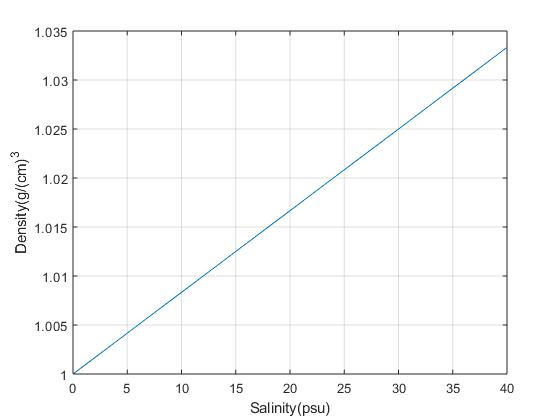
\includegraphics{code/graphs/graph_salinity.jpg}
\caption{Dichteveränderung abhängig vom Salzgehalt}
\end{figure}

\begin{figure}
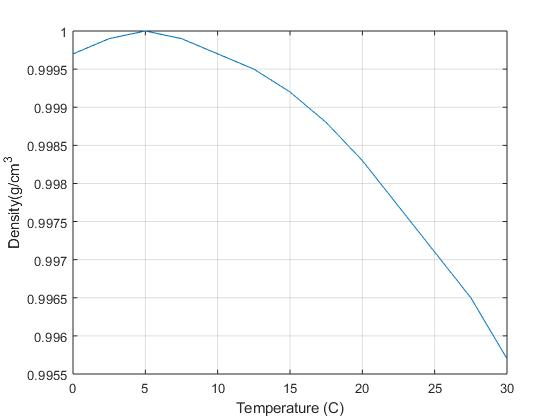
\includegraphics{code/graphs/graph_temp.jpg}
\caption{Dichteveränderung abhängig von der Temperatur}
\end{figure}

Diese Einflüsse Lassen sich in einer Gleichung zusammenfassen, welche im Hauptteil des Buches im Kapitel \ref{Salinität und Dichte} schon Besprochen wurde.

\begin{equation}
\varrho
=
\varrho_0(1-\alpha(T-T_0)+\beta(S-S_0))
\label{skript:salinity-linear}
\end{equation} 

Mittels dieser Gleichung lässt sich nun ein Simulation erstellen, mit welcher sich solche Strömungen simulieren lassen.

\subsection{Golfstrom}
\rhead{Golfstrom}

Im Rahmen dieser Arbeit habe ich versucht den Golfstrom, welcher Europa direkt beeinflusst, zu Simulieren.
Als fokussieren ich hier nur auf einen kleinen Teil der Globalen Thermohalinen Zirkulation.


\begin{figure}
	\includegraphics[]{bilder/deep_ocean_currents.jpg}
\end{figure}

Die Frage ist nun, was passiert mit dem Golfstrom, wenn Klimaerwärmung und Umweltverschmutzung weiter ansteigen?

\subsubsection{Funktionsweise}

Doch zuerst dazu, wie der Golfstrom funktioniert.
Der Golfstrom entspringt im Golf von Mexiko. Von dort aus wird das Warme Wasser von Winden und der Erdrotation nach Norden getrieben.
Auf diesem Weg kühlt das Wasser langsam ab, und wird durch die fortlaufende Verdunstung von Wasser immer salziger. Da der Einfluss der Salinität grösser ist als der der Temperatur, beginnt das Wasser im Norden, durch die nun Hohe Dichte abzusinken. Wenn das Wasser dann abgesunken ist, treibt es dem Grund des Meeres entlang bis nach Afrika, was den Kreislauf schliesst.
Wo hat der Klimawandel nun seinen Einfluss?
Um diese Frage zu beantworten, müssen wir weiter zurückschauen, genauer gesagt zum Kap der guten Hoffnungen. Denn eigentlich beginnt die Strömung schon dort. 
Dort Stellt sich die Frage, in welcher Richtung der Indische Ozean und der Atlantik ihr Salz austauschen. 
Denn eine Veränderung der Salzbilanz könnte im Norden, also vor der Küste Grönlands für eine Störung des Absinkens sorgen, und so den Strom zum erliegen bringen. 
Eine Störung der Salzzufuhr könnte also den Golfstrom zum erliegen bringen.
Hier gehen die Meinungen der Forscher jedoch auseinander. Salzmessungen im offenen Meer sind sehr schwierig. 
Im Moment zeigen diese jedoch, dass der Golfstrom weiter Salz in den Atlantik importiert und sich so selber am leben erhält.

Weiter kommt da noch die Erhöhung des CO2-Gehaltes in der Luft und die somit einhergehende Klimaerwärmung. sie hat zwei direkte Auswirkungen auf den Golfstrom:

\begin{itemize}
	\item Durch die Erhöhung der Lufttemperatur kann das Wasser auf dem Weg in den Norden nicht mehr genug abkühlen, um danach abzusinken.
	\item Das Abschmelzen der Polkappen, welches viel Frischwasser freisetzt, kann die Salzkonzentration so weit verringern, dass das Wasser, aufgrund der reduzierten Dichte, nicht mehr absinken kann.
\end{itemize}

Diese Beiden Prozesse, wären alleine in der Lage den Golfstrom zu stören, doch zusammen ist die Wirkung noch viel schlimmer.

Laut einer Studie des Forschers Liu Wei von der Universität Yale vom 04 Jan 2017 könnte dieses Szenario in den nächsten 300 Jahren tatsächlich eintreten. Sie zeigen auf, dass falls sich die Rate seit 1990 verdoppelt, der Golfstrom in den nächsten 300 Jahren versiegen könnte.

\subsubsection{Folgen}

Was passiert, falls der Golfstrom zum erliegen kommt, oder sogar seine Richtung ändert.
Ich denke der Film "The day after tomorrow" von Roman Emmerich ist bekannt. Er zeigt was passieren könnte, falls der Golfstrom zum erliegen kommt. 
Im Film versinkt innert weniger Tage die ganze Welt in einer neuen Eiszeit un alles endet im Chaos. 
Das ist natürlich ein wenig übertrieben Dargestellt, doch die Richtung stimmt. Falls der Golfstrom stoppt, würde trotz Klimaerwärmung Nordeuropa um einige Grad kälter werden.













	
	
	
	
	
	
	
	
	
	
	
	
	
\end		% *
%
% wuk.tex -- Wetter und Klima
%
% Einleitungskapitel, welches das Wetter- und Klimasystem der Erde in
% qualitiativer Form beschreibt
%
% (c) 2018 Prof Dr Andreas Müller, Hochschule Rapperswil
%
\chapter{Wetter und Klima\label{chapter:wetter und klima}}
\lhead{Wetter und Klima}
US Präsident Donald Trump war schon immer ein Klimaverweigerer, wie Tweets
aus der Zeit lange bevor er Präsident wurde:
\begin{center}
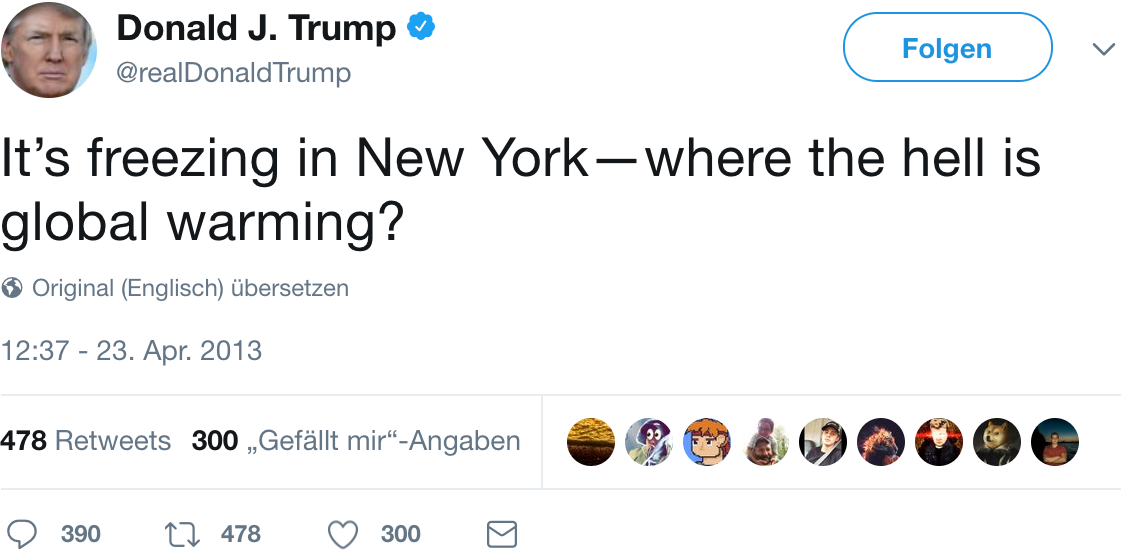
\includegraphics[width=\hsize]{chapters/1/trump.png}
\end{center}
Ganz offensichtlich versteht Trump den Unterschied zwischen Wetter und
Klima nicht.
Ziel dieses Kapitels ist, den Unterschied zwischen Wetter und Klima
zu klären.
Es ist allgemein bekannt, dass auch die besten Wetterprognosen im
günstigsten Fall für einige Tage zutreffen.
Daher soll in diesem Kapitel auch gezeigt werden, warm trotz dieser
Schwierigkeit das Klima sehr wohl langfristig modelliert und prognostiziert
werden kann.
Aus diesen Überlegungen wird auch klar, auf welche Aspekte des Klimasystems
sich ein Klima-Modell fokusieren muss, wenn eine langfristige Prognose
ermöglicht werden soll.

%
% klima.tex -- Klima
%
% (c) 2018 Prof Dr Andreas Müller, Hochschule Rapperswil
%

\section{Klima\label{section:klima}}
\rhead{Klima}
In der Wikipedia kann man die folgenden Definitionen für die Begriffe Wetter
und Klima finden:

\begin{definition}
Als {\em Wetter} bezeichnet man den
spürbaren, kurzfristigen Zustand der Atmosphäre (auch: messbarer
Zustand der Troposphäre) an einem bestimmten Ort der Erdoberfläche,
der unter anderem als Sonnenschein, Bewölkung, Regen, Wind, Hitze
oder Kälte in Erscheinung tritt
\cite{skript:wetter}.
\end{definition}

\begin{definition}
Das {\em Klima} steht als Begriff für die Gesamtheit aller meteorologischen
Vorgänge, die für die über Zeiträume von mindestens 30 Jahren
regelmässig wiederkehrenden durchschnittlichen Zustände der Erdatmosphäre
an einem Ort verantwortlich sind
\cite{skript:klima}.
\end{definition}

Was also Donald Trump in seinem Tweet beschrieben hat ist das Wetter.
Selbst wenn die Temperatur in New York unter den Gefrierpunkt fällt, 
heisst das nicht, dass die mittlere Temperatur in New York über mehrere
Jahre nicht doch ansteigen kann.
Tatsächlich bedeutet ``globale Erwärmung'' nicht, dass die mittlere
Temperatur an jedem Punkt der Erde zunehmen wird.
Im Gegenteil ist es durchaus möglich, dass zwar die mittlere Temperatur
der Erde ständig zunimmt, wie wir in den letzten Jahren auch messtechnisch
nachweisen konnten, dass aber auch die Temperaturunterschiede stark zunehmen,
so dass es am Ende an einzelnen Stelle der Erdoberfläche zu einer 
Abkühlung kommen kann.
Um dieser Komplexität Rechnung zu tragen, spricht man nicht mehr von
der ``globalen Erwärmung'', sondern vom Klimawandel.

Auch wenn das Wetter nur sehr eingeschränkt vorhersagen lässt,
bedeutet das noch lange nicht, dass das Klima nicht doch sehr
genau vorhergesagt werden kann.
Eine Analogie kann den Unterschied zwischen der Vorhersagbarkeit
von Wetter und Klima verdeutlichen.
Wenn man in einem Kochtopf Wasser zum Kochen bringt, stellt sich
eine unverrhersagbare chaotische Bewegung kleiner und grosser
Gasblasen ein.
Es ist unmöglich vorherzusagen, wann und wo sich die nächste Blase
bilden wird und welchen Weg sie an die Oberfläche des Wasser nehmen
wird.
Wenn wir aber nur die mittlere Temperatur betrachten, können wir
aus der Heizleistung der Kochplatte, der Masse und der spezifischen
Wärmekapazität des Wassers genau berechnen, welche Temperatur zu welcher
Zeit im Wasser herschen wird und wir können den Zeitpunkt exakt
vorhersagen, wann das Wasser zu sieden beginnt.
Die mittlere Temperatur des Wassers beschreibt das ``Klima''
in der Pfanne, die kleinräumigen und kurzfristigen Blasen und anderen
Turbulenzen beschreiben das ``Wetter''.


%
% physik.tex -- Physikalische Eigenschaften des Klimasystems
%
% (c) 2018 Prof Dr Andreas Müller, Hochschule Rapperswil
%

\section{Physikalische Eigenschaften des Klimasystems\label{section:physik}}
\rhead{Physikalische Eigenschaften des Klimasystems}
In diesem Abschnitt stellen wir die physikalischen Eigenschaften
aller wesentlichen Komponenten des Klimasystems zusammen.
Dabei geht es zunächst nur darum, die grundlegende Physik in 
Erinnerung zu rufen und die Naturgesetze, die die Wechselwirkungen
zwischen den Komponenten beschreiben.
Auf die Details der mathematischen Modellierung der zukünftigen
Veränderung dieser Grössen werden wir erst später eingehen.

\subsection{Wärme, Konvektion, Kondensation}
Die wohl wichtigste Klima-Grösse ist die Temperatur.
Sie drückt aus, wieviel Energie in Form von Wärme ein Körper oder eine
Komponente des Klimasystems enthält.

\subsubsection{Wärmekapazität}
Die spezifische Wärme $C$ gibt an, wie die innere Energie $U$ sich bei
einer Temperaturänderung $\Delta T$ verändert:
\[
\Delta U = C\cdot\Delta T.
\]
Der Körper speichert Energie in Form der thermischen Bewegung der
einzelnen Atome.
Schwerere Atome können bei gleicher Bewegungsgeschwindigkeit 
mehr Energie speichern.
Stoffe mit grösserer Dichte können mehr Atome und damit auch mehr
Wärmeenergie in einem kleineren Volumen unterbringen.
Die spezifische Wärmekapazität $c$ gibt an, welche Wärmekapazität
ein Kilogramm eines Stoffes hat.
Ein Körper der Masse $m$ hat also die Wärmekapazität $C=c\cdot m$.

\subsubsection{Wärmeleitung\label{subsection:heatconduction}}
Herrschen in einem Körper Temperaturunterschiede, ist $T$ nicht mehr
nur eine Konstante sondern eine Funktion $T(x,y,z,t)$
der Koordinaten und auch der Zeit.
Temperaturunterschiede werden sich ausgleichen, indem Energie von
wärmeren zu kälteren Teilen des Körpers fliegt.
Dies geschieht umso schneller, je grösser die Unterschiede sind.
Die Wärmeleitungsgleichung
\begin{equation}
\frac{\partial T}{\partial t}
=
\kappa
\biggl(
\frac{\partial^2}{\partial x^2}
+
\frac{\partial^2}{\partial y^2}
+
\frac{\partial^2}{\partial z^2}
\biggr)
T
\label{skript:waermeleitung}
\end{equation}
beschreibt die Entwicklung der Funktion $T(x,y,z,t)$ an jedem
Ort des Raumes \cite{skript:waermeleitung}.
Der Koeffizient $\kappa$ ist eine Materialkonstante, die beschreibt,
wie schnell sich die Temperaturunterschiede ausgleichen können.
Ist $\kappa=0$, folgt $\partial T/\partial t=0$, die Temperatur 
ändert sich nicht, es findet keine Wärmeleitung statt.

Die rechte Seite von \eqref{skript:waermeleitung} kann mit dem
sogenannten Laplace-Operator gemäss der folgenden Definition 
geschrieben werden.

\begin{definition}
Der Operator
\[
\Delta
=
\frac{\partial^2}{\partial x^2}
+
\frac{\partial^2}{\partial y^2}
+
\frac{\partial^2}{\partial z^2}
\]
heisst der
{\em Laplace-Operator}.
\end{definition}

Die Wärmeleitungsgleichung erhält damit die Form
\begin{equation}
\frac{\partial T}{\partial t}
=
\kappa\Delta T.
\label{skript:waermeleitung2}
\end{equation}
In einer Dimension wird daraus
\[
\frac{\partial T}{\partial t} = \kappa \frac{\partial^2 T}{\partial x^2}.
\]
Die Änderung der Temperatur ist also umso grösser, je grösser
die Krümmung der Temperaturkurve $x\mapsto T(x,t)$ ist.
Die Wärmeleitungsgleichung beschreibt also, wie sich die Temperaturen
ausgleichen, bis nur noch lineare Temperaturgradienten bestehen bleiben.

\subsubsection{Randbedingungen}
Die partielle Differentialgleichung~\eqref{skript:waermeleitung2}
alleine legt die Temperaturverteilung noch nicht fest.
Vielmehr muss man ausserdem die Temperatur zur willkürlich als $t=0$
gewählten Anfangszeit kennen, und die Temperatur am Rand des
Definitionsgebietes.
Erst zusammen mit diesen Randbedingungen ist die Lösung eindeutig festgelegt.

\subsubsection{Konvektion}
Wärmeleitung kann Wärmeenergie nur vergleichsweise langsam transportieren.
Das einleitende Beispiel des Kochtopfs zeigt auch, wie ein effizienterer
Energietransport funktionieren kann.
In der Atmosphäre dehnt sich warme Luft aus.
Dank der geringeren Dichte können warme Luftblasen aufsteigen und damit
Wärme viel effizienter in die obere Atmosphäre transportieren
als dies mit Wärmeleitung möglich wäre.
Dieser Prozess heisst {\em Konvektion} \cite{skript:konvektion}.
\index{Konvektion}%

\subsubsection{Advektion}
Wir wollen den Fall eines strömenden Mediums mathematisch etwas genauer
ausarbeiten.
Bewegt sich das Medium mit der Geschwindigkeit $\vec v$, dann ändert sich
die Temperatur des Mediums, welches sich über dem Punkt $P=(x,y,z)$
befindet.
Nach der Zeit $\Delta t$ befindet sich derjenige Teil des Mediums
über dem Punkt $P$, der sich vorher über dem Punkt $P-\Delta t\cdot\vec v$
befand.
Die Temperatur zur Zeit $t+\Delta t$ ist daher
$T(P,t+\Delta t)=T(P-\vec{v}\,\Delta t,t)$.
Die Temperaturänderung ist
\begin{align*}
T(P,t+\Delta t)
&=
T(P,t) + (T(P,t+\Delta t)-T(P,t))
=
T(P,t) + T(P-\vec v\,\Delta t, t)-T(P,t)
\\
\intertext{und damit die Temperaturänderung pro Zeiteinheit}
\frac{
T(P,t+\Delta t)
-
T(P,t)
}{\Delta t}
&=
\frac{
T(P-\vec{v}\,\Delta t, t)-T(P,t)
}{\Delta t}.
\end{align*}
Beim Grenzübergang $\Delta t\to 0$ wird aus der linken Seite die
partielle Ableitung nach $t$.
Die rechte Seite kann mit Hilfe der Kettenregel berechnet weren.
Es wird
\begin{equation}
\frac{\partial T}{\partial t}
=
-
\frac{\partial T}{\partial x} v_x
-
\frac{\partial T}{\partial y} v_y
-
\frac{\partial T}{\partial z} v_z.
\label{skript:advektion1}
\end{equation}
Der Ausdruck auf der rechten Seite kann vektoriell mit der folgenden
Definition etwas eleganter geschrieben werden.

\begin{definition}
Der vektorielle Operator 
\[
\nabla
=
\def\arraystretch{1.3}
\begin{pmatrix}
\frac{\partial}{\partial x}\\
\frac{\partial}{\partial y}\\
\frac{\partial}{\partial z}
\end{pmatrix}
\]
heisst der {\em Nabla-Operator}.
Der Vektor
\[
\nabla f
=
\def\arraystretch{1.3}
\begin{pmatrix}
\frac{\partial f}{\partial x}\\
\frac{\partial f}{\partial y}\\
\frac{\partial f}{\partial z}
\end{pmatrix}
=
\operatorname{grad} f
\]
heisst der {\em Gradient} von $f$.
Das Skalarprodukt $\nabla\cdot\vec{v}$ ist ein Skalar, die
{\em Divergenz}
eines Vektorfeldes $\vec{v}$, sie wird manchmal auch
$\operatorname{div}\vec{v}$ geschrieben.
\end{definition}
\index{Gradient}%
\index{Divergenz}%
\index{Nabla-Operator}%

Die Temperaturänderung in Folge der Strömung 
\eqref{skript:advektion1}
wird 
\begin{equation}
\frac{\partial T}{\partial t}
=
-\vec{v}\cdot\nabla T.
\label{skript:advektion2}
\end{equation}
\index{Advektion}%
Man nennt diese Temperaturänderung durch die Strömung auch
{\em Advektion}.
Die Wärmeleitungsgleichung kann damit zu einem umfassenderen
Modell
\begin{equation}
\frac{\partial T}{\partial t}
=
-\vec{v}\cdot\nabla T +\kappa\Delta T
\label{skript:waermeleitungadvektion}
\end{equation}
zusammengefasst werden.
Es ist geeignet für die Beschreibung sowohl der Atmosphäre wie auch des
Wärmeaustausches in den Ozeanen.

\subsubsection{Phasenübergänge}
Um ein Kilogramm Wasser bei $20^\circ\text{C}$ zu verdunsten, ist eine
latente Wärme von $2480\,\text{kJ}$ nötig.
\index{latente Wärme}%
Um ein Kilogramm Luft um ein Grad zu erwärmen, sind dagegen nur
$1.005\,\text{kJ}$ notwendig.
Anders herum bedeutet dies, dass eine mit Wasserdampf angereicherte Atmosphäre
sehr viel mehr Energie in Form von latenter Wärme speichern kann, als
allein durch die Wärmekapazität trockener Luft möglich wäre.
\index{latente Wärme}%

Wir haben damit zwei Mechanismen identifiziert, wie eingestrahlte
und in der Erdkruste als Wärme gespeicherte Energie in die Atmosphäre 
transportiert werden kann.
Einerseits kann Luft über aufgewärmten Landmassen oder dem Meer erwärmt
werden und als Konvektionsströmung aufsteigen.
Andererseits kann Wasser an der Oberfläche verdampft werden und damit die
latente Wärme in die Atmosphäre übergehen.
Man nennt diese Mechanismen auch turbulente Flüsse
\cite[S.~70]{skript:wiefunktioniertdas}.
\index{turbulente Flüsse}%

Der Wassergehalt der Luft kann höchstens einige wenige Prozente betragen.
Zwar ist die Wärmespeicherung durch Verdunstung über 2000 mal effizienter,
aber weil nur wenig Wasser dafür zur Verfügung steht, übernimmt die Verdunstung
doch nicht einen derart grossen Teil des Energietransports von der
Oberfläche in die Atmosphäre.
In der Tat finden etwa 30\% des Energietransports von der Erdkruste
in die Atmosphäre durch turbulente Flüsse statt, davon etwa
7\% durch Konvektion und 23\% durch latente Wärme
\cite[S.~70]{skript:wiefunktioniertdas}.
Höhere Temperaturen begünstigen die Verdunstung und verschieben diesen
Anteil zugunsten der latenten Wärme.
Man darf also davon ausgehen, dass höhere Oberflächentemperaturen
zu einem überproportional höheren Energietransport in die Atmosphäre
führen.

In der Atmosphäre kann die Energie über grosse Distanzen transportiert
und später wieder freigesetzt werden, wie Hurricanes und Tornadoes
eindrücklich demonstrieren können.
Damit ein Klimamodell Aussagen machen kann über das Auftreten von
extremen Wetterphänomenen muss es also den Wassergehalt der
Atmosphäre modellieren.
In Kapitel~\ref{chapter:planeten} wird gezeigt, wie man hierzu vorgehen
könnte.

\subsection{Strahlung\label{skript:grundlagen:strahlung}}
Der bedeutendste Energietransportmechanismus in der Atmosphäre ist
die Strahlung.
In diesem Abschnitt stellen wir die Strahlungsgesetze zusammen und
studieren die Strahlungsbilanz der Atmosphären.

\subsubsection{Schwarzkörperstrahlung}
\index{schwarzer Körper}%
Die Strahlung der Sonne wie auch der Erde kann als Strahlung eines
schwarzen Körpers modelliert werden.
Ein schwarzer Körper ist ein idealisierter Körper, der alle auftretende
Strahlung absorbieren kann \cite{skript:schwarzerkoerper}.
Er befindet sich im thermischen Gleichgewicht mit dem Strahlungsfeld,
seine Strahlung hängt daher nur von der Temperatur ab.

\subsubsection{Stefan-Boltzmann-Gesetz}
Das {\em Stefan-Bolzmann-Gesetz} gibt Auskunft darüber, wieviel
\index{Stefan-Boltzmann-Gesetz}
Energie insgesamt von einem schwarzen Körper abgestrahlt wird.
Die gesamte Strahlung hängt natürlich von der Oberfläche $A$ des Strahlers ab,
aber die Strahlungsleistung pro Flächeneinheit hängt
nur noch von der
Temperatur ab.
Die gesamte Strahlungsleistung ist
\begin{equation}
P=\sigma AT^4
\qquad \text{mit}\qquad
\sigma=5.670367\cdot10^{-8}\frac{\text{W}}{\text{m}^2\text{K}^4}.
\label{skript:stefon-boltzmann}
\end{equation}

\subsubsection{Sonne}
Wir wenden das Stefan-Boltzmann-Gesetz auf die Strahlung der Sonne an.
A priori ist nicht klar, dass das Strahlungsspektrum der Sonne tatsächlich
als das eines schwarzen Körpers modelliert werden kann, doch die
Abbildung~\ref{skript:strahlungsspektrum} zeigt, dass das Schwarzkörperspektrum
mindestens eine sehr gute Approximation des tatsächlichen Spektrums ist.

Die Strahlung der Sonne nimmt mit dem Quadrat der Entfernung ab.
Von der Strahlungsleistung $\sigma T^4$ pro Flächeneinheit der
Sonnenoberfläche bleibt in der Entfernung der Erde die Leistung
\begin{equation}
P_{\earth}
=
\sigma T^4\cdot \biggl(\frac{R_{\astrosun}}{a_{\earth}}\biggr)^2
\label{skript:solarkonstante}
\end{equation}
übrig,
wobei $R_{\astrosun}=6.957\cdot 10^8\text{m}$ der Radius der Sonne ist und
$a_{\earth}=1.496\cdot 10^{11}\text{m}$ die mittlere Entfernung der Erde
von der Sonne.
Setzt man diese Werte und die Temperatur $T=5778\text{K}$ in die Gleichung
\eqref{skript:solarkonstante}
ein, erhält man
\begin{align*}
P_{\earth}
&=
1366.8 \text{W}/\text{m}^2,
\end{align*}
auch bekannt als die {\em Solarkonstante}.
\index{Solarkonstante}

\subsubsection{Wiensches Verschiebungsgesetz}
Die Strahlungsleistung ist nicht über alle Wellenlängen gleichmässig
verteilt.
\index{Wiensches Verschiebungsgesetz}
Das {\em Wiensche Verschiebungsgesetz} besagt, dass die maximale
Strahlungsleistung bei einer Wellenlänge abgestrahlt wird,
die umgekehrt proportional zur Temperatur ist:
\begin{equation}
\lambda_{\text{max}}
=
\frac{b}{T}
\qquad\text{mit}\qquad
b=2.897\cdot10^{-3}\text{m}\cdot\text{K}.
\end{equation}
Für die Oberfläche der Sonne mit $T=5778\text{K}$ findet man die
Wellenlänge
$\lambda_{\text{max}}=5\cdot10^{-7}\text{m} = 500\text{nm}$,
dies entspricht grünem Licht.
Die Strahlung der Erde mit ihrer mittleren Temperatur von 287\,K
hat dagegen ihr Maximum bei $\lambda_{\text{max}}=10\,\mu\text{m}$,
also im Infrarotbereich.

\subsubsection{Strahlung und Reflektion in der Atmosphäre}
Die Strahlungsleistung eines schwarzen Körpers in Abhängigkeit
von der Wellenlänge wird durch das Plancksche Strahlungsgesetz
\begin{equation}
E(\lambda,T)
=
\frac{2\pi hc^2}{\lambda^5}\frac{1}{e^{\frac{hc}{\lambda kT}}-1}
\end{equation}
wiedergeben.
$E(\lambda,T)$ ist die
pro Flächeneinheit des Strahlers und pro Wellenlängeneinheit
abgestrahlte Leistung.
\begin{figure}
\centering
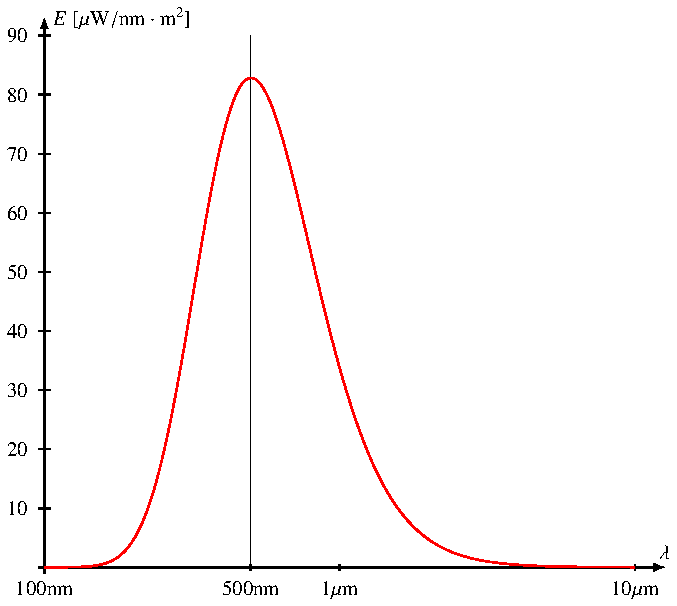
\includegraphics{chapters/1/planck.pdf}
\caption{Plancksches Strahlungsgesetz für die Sonne
\label{skript:planck-kurve}}
\end{figure}
\index{Plancksches Strahlungsgesetz}
\index{Strahlungsgesetz,Plancksches}
Die Strahlungsdichte in Abhängigkeit von der Wellenlänge ist in
Abbildung~\ref{skript:planck-kurve} dargestellt.
Die gesamte Strahlungsleistung ist das Integral
\[
P
=
\int_{0}^\infty E(\lambda,T)\,d\lambda
=
\int_{0}^\infty 
\frac{2\pi hc^2}{\lambda^5}\frac{d\lambda}{e^{\frac{hc}{\lambda kT}}-1}.
\]
Man beachte aber, dass in den graphischen Darstellungen des
Strahlungsspektrums eine logarithmische $\lambda$-Skala
verwendet wird.
Bei grossen Wellenlängen (``rechts'') wird die Kurve also in Wahrheit
viel stärker ausgedehnt.
Will man die Flächeninhalte unter den Kurven vergleichen, muss man
$E(\lambda,T)$ mit dem Faktor $\lambda$ skalieren.

\subsubsection{Einstrahlungswinkel}
Warum ist es in den Tropen wärmer als in gemässigten Breiten oder
an den Polen, wenn
die Sonne doch überall mit der gleichen Intensität einstrahlt.

Der Unterschied stammt natürlich vom Einstrahlungswinkel.
Der Ausdruck \eqref{skript:solarkonstante} für $P_{\earth}$ 
beschreibt die Strahlungsleistung pro Flächeneinheit, doch diese
Flächeneinheit wird senkrecht auf die Ausbreitungsrichtung der
Strahlung gemessen.
In gemässigten Breiten und an den Polen fällt die Strahlung 
in viel kleinerem Winkel auf die Erdoberfläche.
Die einfallende Energie verteilt sich daher auf eine grössere
Fläche.
Ist $\alpha$ der Winkel zwischen der Vertikalen und der Strahlungsrichtung,
dann ist die auf einer Erdoberfläche einfallende Strahlungsdichte nur
noch $P_{\earth}\cdot\cos\alpha$
(siehe auch Abbildung~\ref{skript:einfallswinkel}).

\begin{figure}
\centering
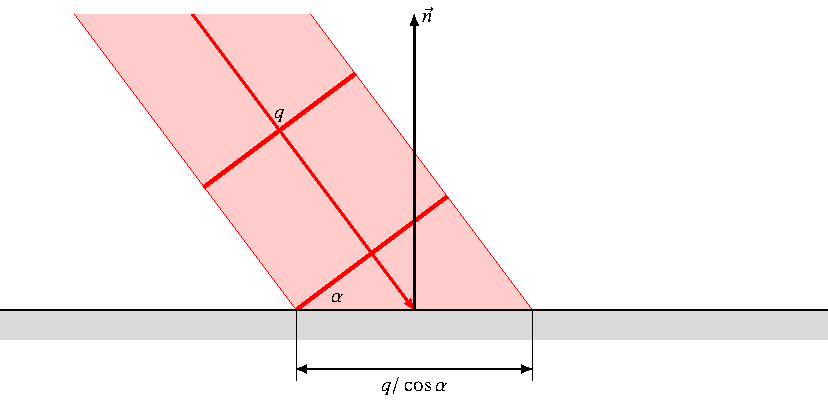
\includegraphics{chapters/1/einfall.pdf}
\caption{Einfluss des Einstrahlungswinkels auf die pro Flächeneinheit
der Erdoberfläche einfallende Strahlungsleistung.
Ein Strahlenbündel mit Querschnitt $q$, welches im Winkel
$\alpha$ zur Vertikalen einfällt, bedeckt die Fläche $q/\cos\alpha$
auf der Erdoberfläche.
\label{skript:einfallswinkel}}
\end{figure}

\subsubsection{Albedo\label{skript:subsubsection:albedo}}
\begin{table}
\centering
\begin{tabular}{|l|l|}
\hline
Material&Albedo\\
\hline
Frischer Schnee&0.8 -- 0.9\\
Wolken         &0.6 -- 0.9\\
Wüste          &0.3\\
Rasen          &0.18--0.23\\
Wald           &0.05--0.18\\
Wasserfläche   &0.05--0.22 (winkelabhängig)\\
Erde           &0.306 \\
Mond           &0.11 \\
\hline
\end{tabular}
\caption{Albedo verschiedener Oberflächen und Himmelskörper
(aus \cite{skript:albedo})
\label{skript:albedotabelle}}
\end{table}
Die Erde ist noch weniger perfekter schwarzer Strahler als die Sonne.
Die Ausstrahlung enthält zwar die Strahlung eines schwarzen Körpers mit
der Mitteltemperatur als Temperatur $T$,
sie ist aber überlagert von der Strahlung, die vom Erdboden oder von
Wolken reflektiert wird.
Die {\em Albedo} ist der Anteil der reflektierten Strahlung, also ein
Wert zwischen $0$ und $1$.
\index{Albedo}
Tabelle~\ref{skript:albedotabelle} stellt einige interessante
Albedo-Werte von verschiedenen Oberflächen zusammen.

Die Albedo hat eine direkte Auswirkung auf das Klima, umgekehrt
hängt die Albedo aber auch vom Klima ab.
Nimmt die Bewölkung zu, steigt die Albedo, es erreicht weniger 
Strahlung die Erdoberfläche.
Schneefall erhöht ebenfalls die Albedo.
Umgekehrt reduziert das Abschmelzen der Polkappen oder der
Schneedecke in Permafrostgebieten die Albedo, so dass mehr Strahlung
von der Erdoberfläche absorbiert wird.

\subsubsection{Strahlungsbilanz}
\begin{figure}
\centering
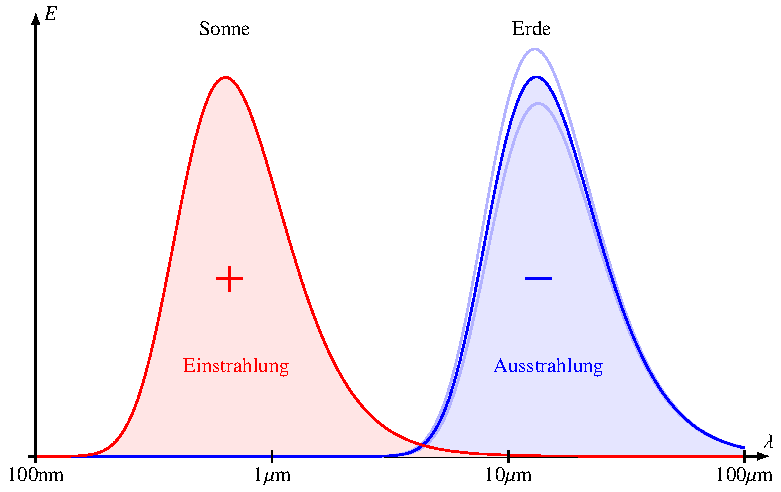
\includegraphics{chapters/1/vergleich.pdf}
\caption{Strahlung der Sonne (rot) und der Erde (blau).
Das Maximum der Strahlung der Sonne ist im sichtbaren Bereich,
das Maximum der Wärmestrahlung der Erde im Infraroten.
\label{skript:strahlung-sonne-erde}}
\end{figure}%
In Abbildung~\ref{skript:strahlung-sonne-erde} sind die Planckschen
Strahlungskurve für die Sonne und Erde derart skaliert dargestellt,
dass die Flächen unter den Strahlungs direkt als Mass für die gesamte
Strahlungsleistung dienen können.
Die rote Kurve zeigt die spektrale Strahlungsleistung, die von der
Sonne auf den Querschnitt $\pi R_{\earth}^2$ der Erde eingestrahlt wird,
also
\[
E(\lambda,T_{\astrosun}) \cdot 2\pi R_{\earth}^2
\cdot
\biggl(\frac{R_{\astrosun}}{a_{\earth}}\biggr)^2
\]
mit $T_{\astrosun}=5778\text{K}$.
Die dunkelblaue Kurve zeigt das Ausstrahlungsspektrum der ganzen Erde mit
einer Temperatur von $T=279\text{K}$, also
\[
E(\lambda,T_{\earth})\cdot 4\pi R_{\earth}^2.
\]
Die Fläche unter der Kurve ist ein Mass für die gesamte Energie.
Offenbar halten sich Einstrahlung und Ausstrahlung die Waage.

Die Einstrahlung kann sich zum Beispiel dann verändern, wenn 
mehr Strahlung reflektiert wird.
Die Ausstrahlung dagegen verringert sich, wenn die Atmosphäre für infrarote
Strahlung undurchsichtiger wird, wie dies zum Beispiel durch
erhöhte $\text{H}_2\text{O}$- oder $\text{CO}_2$-Konzentration geschehen kann.
Damit sich wieder ein Gleichgewicht einstellt, muss sich die Temperatur der
Erde erhöhen, damit die Ausstrahlung ebenfalls höher wird
(obere hellblaue Kurve in Abbildung~\ref{skript:strahlung-sonne-erde}).
Sinkt der Gehalt an Treibhausgasen, wird die Atmosphäre transparenter
für Wärmestrahlung,
ein Gleichgewicht ist möglich bei tieferer Temperatur (untere
hellblaue Kurve).
Diese Abhängigkeit der Temperatur von der Transparenz der
Atmosphäre für Wärmestrahlung ist bekannt als der {\em Treibhauseffekt}.
\index{Treibhauseffekt}

\subsubsection{Tatsächliches Strahlungspektrum}
\begin{figure}
\centering
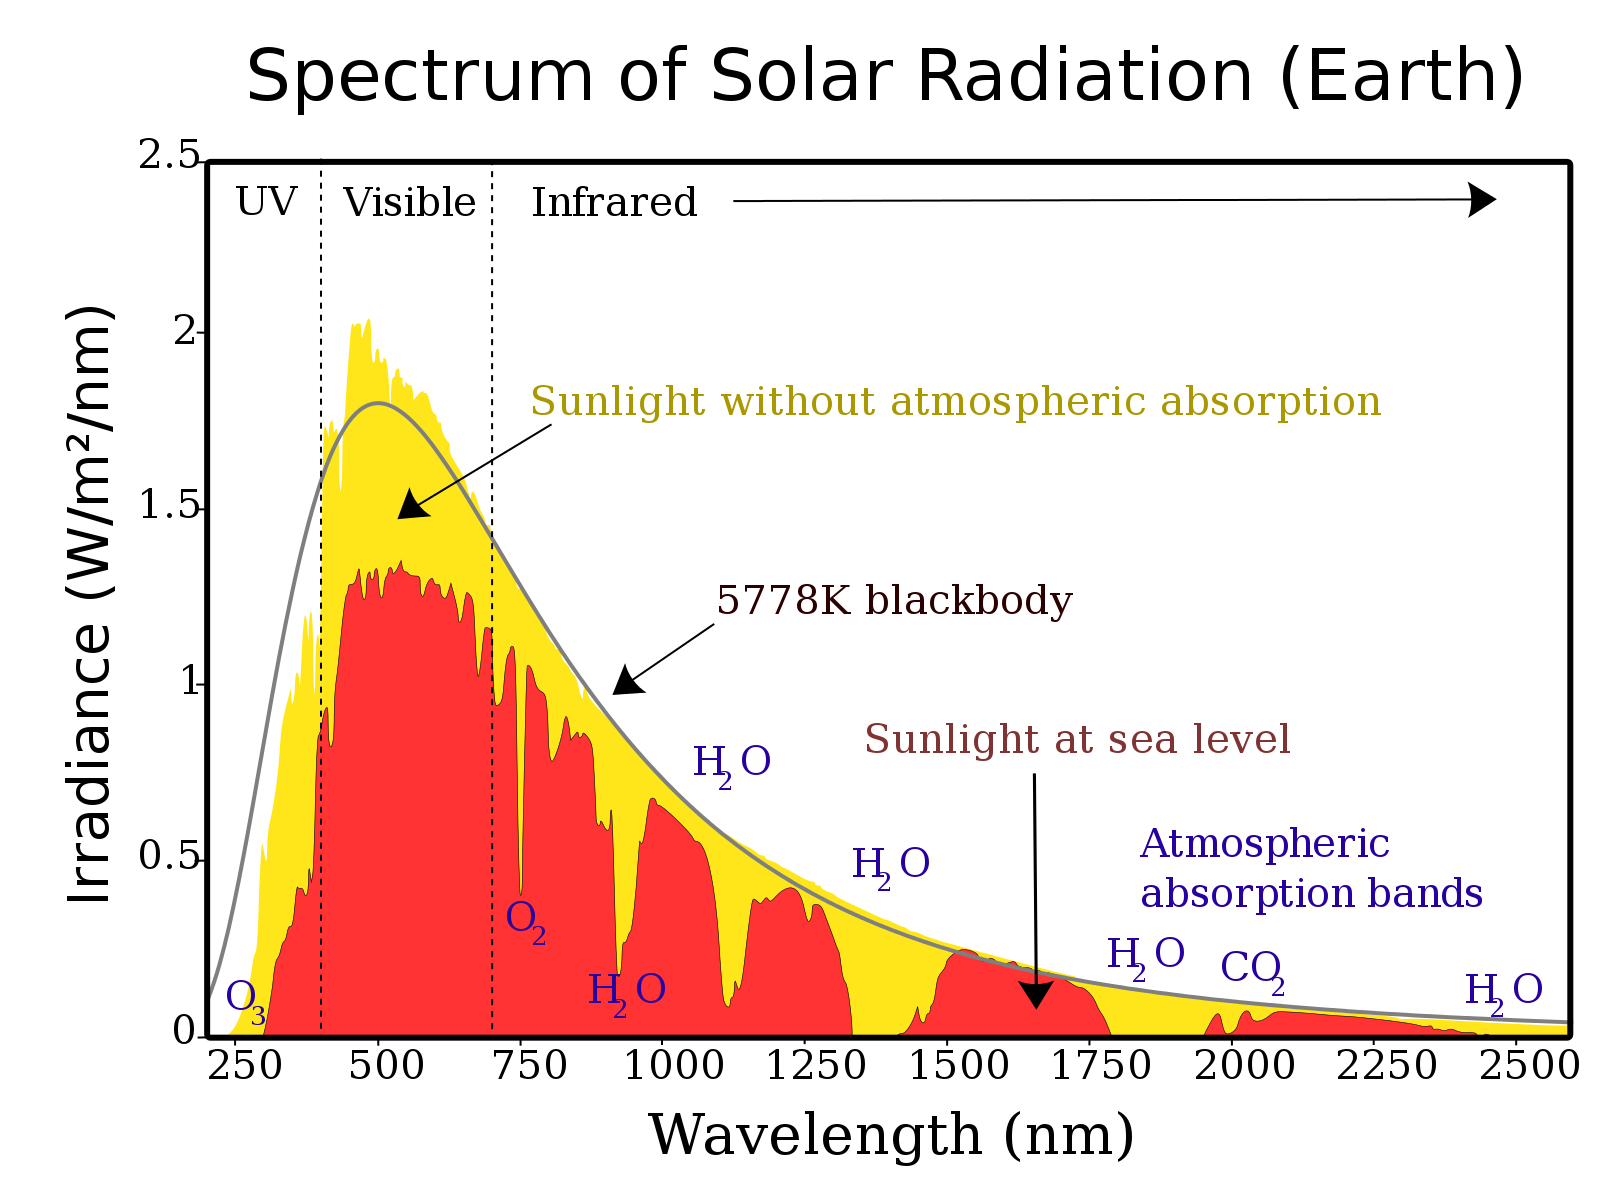
\includegraphics[width=0.7\hsize]{chapters/1/Solar_spectrum_en.png}
\caption{Tatsächliches Spektrum der Sonnenstrahlung mit (rot) und
ohne (gelb) atmosphärische Absorbtion im Vergleich mit dem Spektrum
der Schwarzkörperstrahlung \cite{skript:sunlight}.
\label{skript:strahlungsspektrum}}
\end{figure}
In Abbildung~\ref{skript:strahlungsspektrum} ist das tatsächlich gemessene
Strahlungsspektrum der Sonne dargestellt.
Es fällt auf, dass Wasserdampf und $\text{CO}_2$  für bedeutende
Absorbtionsbänder im Infraroten verantwortlich ist,
während im sichtbaren bereich
die Absorbtion sehr gleichmässig ist.

\subsection{Erdrotation und atmosphärische Zirkulation\label{skript:section:zirkulation}}
Die Einstrahlung ist wegen des grösseren Einstrahlungswinkels
am grössten am Äquator, während an den Polen die Ausstrahlung überwiegt.
Dies führt dazu, dass die Temperatur an den Polen tiefer ist.
Da sich die Erde im Gleichgewicht befindet, bedeutet dieser
Temperaturunterschied aber auch, dass Prozesse in
der Atmosphäre Energie aus niedrigen Breiten zu den Polen
transportieren müssen.
Die Temperaturunterschiede sind jedoch zu klein dafür, dass Wärmeleitung
den Transport bewerkstelligen könnte.
Die Energie muss daher durch Advektion (S.~\pageref{skript:advektion})
unterstützt von latenter Wärme transportiert werden.
Um den Energiehaushalt des globalen Klimasystems zu verstehen, muss
\index{globale Zirkulation}%
\index{Zirkulation, globale}%
man daher die globalen Strömungen in der Atmosphäre aber auch in
den Ozeanen verstehen.

In Kapitel~\ref{chapter:fluiddynamik} werden die Grundgleichungen
der Fluiddynamik besprochen.
In diesem Abschnitt beschränken wir uns auf eine qualitative
Diskussion der globalen Zirkulation.
Die globale Zirkulation unterscheidet sich von Strömungen, die 
in technischen Anwendungen üblicherweise studiert werden dadurch,
dass sie zwar im allgemeinen langsamer ist, dafür aber ein viel grössers
Volumen und grössere Distanzen umfasst.
Die Windsysteme, die für die Wetterphänomene verantwortlich sind,
haben typische Abmessungen von hunderten oder sogar tausenden von
Kilometern.

\subsubsection{Druckunterschiede und Euler-Wind}
Windströmungen in der Atmosphäre werden von Druckunterschieden
hervorgerufen.
Die Sonnenstrahlung erwärmt die Erdoberfläche und mittelbar die
Atmosphäre.
Die warme Luft hat geringere Dichte und steigt daher auf.
Damit nimmt die Kraft ab, die die Luft auf darunterliegenden
Schichten ausüben kann, es entsteht ein Unterdruck.
Man nennt eine Luftströmung, die nur durch Druck\-unterschiede
unter Vernachlässigung von Corioliskraft, Zentrifugalkraft und
Reibung entsteht, den {\em Euler-Wind}.
\index{Euler-Wind}
Lokale Wind-Systeme wie Land-See-Wind oder Berg-Tal-Wind sind von
dieser Art.

\subsubsection{Coriolis-Effekt}
\index{Coriolis-Kraft}%
\index{Coriolis-Effekt}%
Die Erde dreht sich in 23 Stunden 56 Minuten und 4.091 Sekunden
einmal um sich selbst (siderische Rotationsperiode).
\index{siderische Rotationsperiode}%
Die Drehung kann mit dem Winkelgeschwindigkeitsvektor
$\vec{\Omega}$
beschrieben werden, der die Richtung der Erdachse vom Süd- zum Nordpol
hat und als Länge die Winkelgeschwindigkeit
\[
\omega
=
|\vec{\Omega}|
=
\frac{2\pi}{86164.091\,\text{s}}.
\]
Ein Körper, der sich relativ zu einem mit der Erde verbundenen
Koordinatensystem mit der Geschwindigkeit $\vec{v}$ bewegt,
erlebt eine durch die Drehung verursachte Coriolis-Beschleunigung
\[
\vec{a} = -2\vec{\Omega}\times\vec{v}.
\]
Ein Flugzeug, welches mit 880\,km/h über den Nordpol fliegt,
erfährt dort die Beschleunigung 
\[
|\vec{a}|
=
\biggl|
-2
\cdot
\frac{2\pi}{86164.091\,\text{s}}
\cdot
244.44\frac{\text{m}}{\text{s}}
\biggr|
=
0.01782\frac{\text{m}}{\text{s}^2}.
\]
Diese Beschleunigung ist viel zu klein, dass sie einen wesentlichen
Einfluss auf die Bahn eines Flugzeugs haben könnte.
Der Luftwiderstand und die von den Steuerflächen des Flugzeugs erzeugten
Kräfte und die daraus resultierenden Beschleunigungen sind
um Grössenordnungen grösser.
In der freien Atmosphäre wirkt auf die Luft jedoch nur die Druckkraft,
so dass die Coriolis-Beschleunigung einen dominanten Einfluss bekommt.

\begin{figure}
\centering
\begin{tikzpicture}[scale=1, >= latex]
\node at (0,0) {
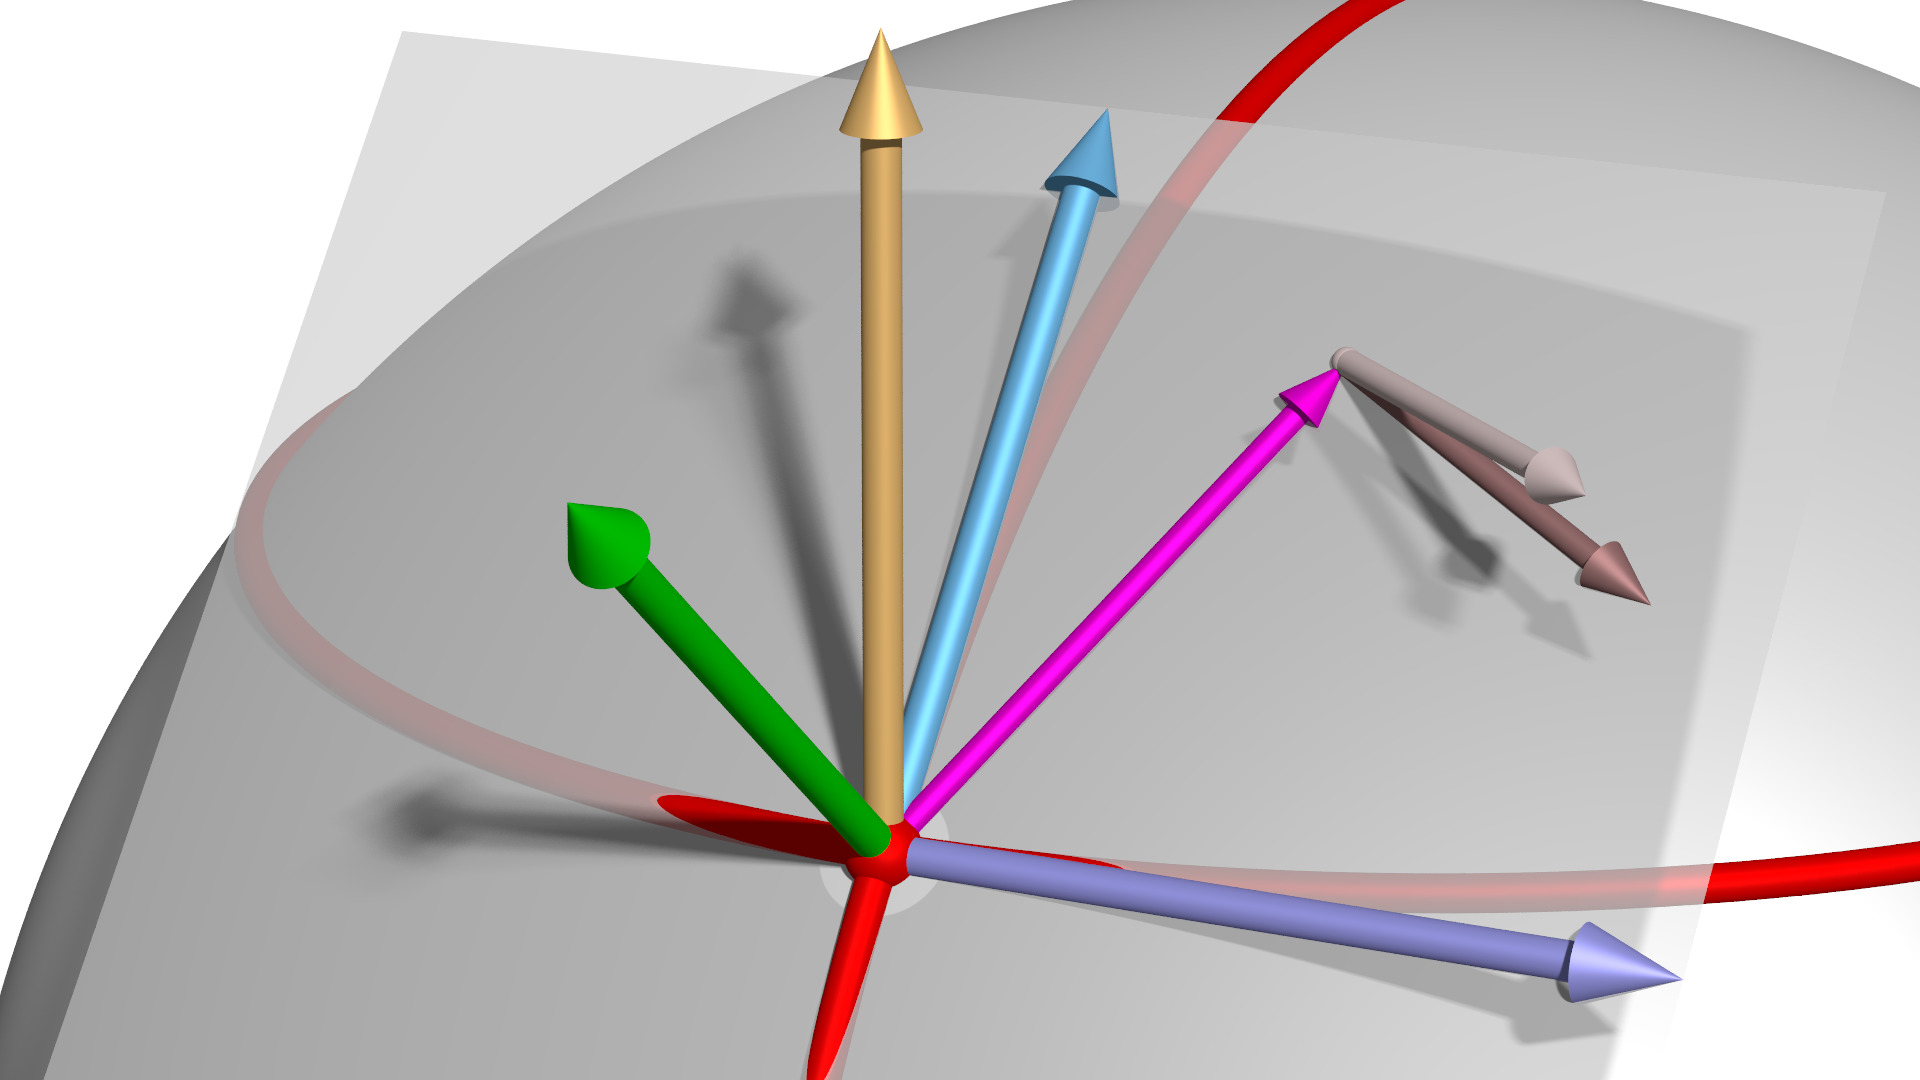
\includegraphics[width=\hsize]{chapters/1/betaplane.jpg}
};
%\node at (0,0) {$\bullet$};
%\node at (1,0) {$\bullet$};
%\node at (-1,0) {$\bullet$};
%\node at (0,1) {$\bullet$};
%\node at (0,-1) {$\bullet$};
\node at (-0.3,-2.7) {$B$};
\node at (5.1,-2.7) {$U$};
\node at (1.4,2.9) {$V$};
\node at (-0.6,4.1) {$\vec{\Omega}$};
\node at (-3,0.6) {$\vec{n}$};
\node at (2.3,1.4) {$\vec{v}$};
\node at (4.5,1) {$-2\vec{\Omega}\times\vec{v}$};
\node at (6,-0.5) {$(-2\vec{\Omega}\times\vec{v})_{\|}$};
\end{tikzpicture}
\caption{$\beta$-Ebene: Koordinatensystem in der Tangentialgebene an die Kugel
im Punkt $B$ mit Achsen $U$ parallel zu Breitenkreisen und $V$ parallel
zu Längenkreisen.
Die Normale der Tangentialebene ist $\vec{n}$.
Ebenfalls eingezeichnet die Coriolis-Beschleunigung
$-2\vec{\Omega}\times\vec{v}$ zur Geschwindigkeit $\vec{v}$ und
die Komponente $(-2\vec{\Omega}\times\vec{v})_{\|}$ parallel
zur Tangentialebene.
\label{skript:betaplane}}
\end{figure}
Die grossräumige Strömung in der Erdoberfläche verläuft im Wesentlichen 
parallel zur Erdoberfläche.
Daher interessiert für die Beschreibung der Wirkung des Coriolis-Effekts
vor allem die Komponente der Beschleunigung parallel zur Erdoberfläche.
In einem Punkt $B$ der Erdoberfläche verwenden wir daher ein
Koordinatensystem in der Tangentialebene so, dass die $x$-Achse tangential
zum Breitenkreis in $B$ ist und die $y$-Achse tangential zum Längenkreis
(Abbildung~\ref{skript:betaplane}).
Die tangentiale Geschwindigkeit wird in diesem Koordinatensystem durch die
Komponenten $u$ in $U$-Richtung und $v$ in $V$-Richtung beschrieben.
Dieses Koordinatensystem in der Tangentialebene im Punkt $B$ heisst auch
die {\em $\beta$-Ebene}.
\label{skript:betaplane:definition}
\index{$\beta$-Ebene}

Wir berechnen die Coriolis-Beschleunigung in diesem Koordinatensystem.
Für einen Geschwindigkeitsvektor $\vec{v}$ parallel zu $V$ hat das
Vektorprodukt $\vec{\Omega}\times \vec{v}$ bereits die Richtung $U$,
er muss also nicht mehr in die Tangentialebene projiziert werden.
Der Winkel zwischen $\vec{\Omega}$ und $V$ ist die geographischen Breite
$\alpha$.
Die Coriolis-Beschleunigung ist daher $2\omega \sin(\alpha)u\cdot V$.

Für einen Geschwindigkeitsvektor $\vec{v}$ parallel zu $U$ steht
das Vektorprodukt $-2\vec{\Omega}\times\vec{v}$ senkrecht auf 
der Erdachse.
Da $U$ und $\vec{\Omega}$ senkrecht stehen, ist der Betrag der 
Coriolis-Beschleunigung
\[
|\text{$-2\vec{\Omega}\times\vec{v}$}|
=
2\omega u.
\]
\begin{figure}
\centering
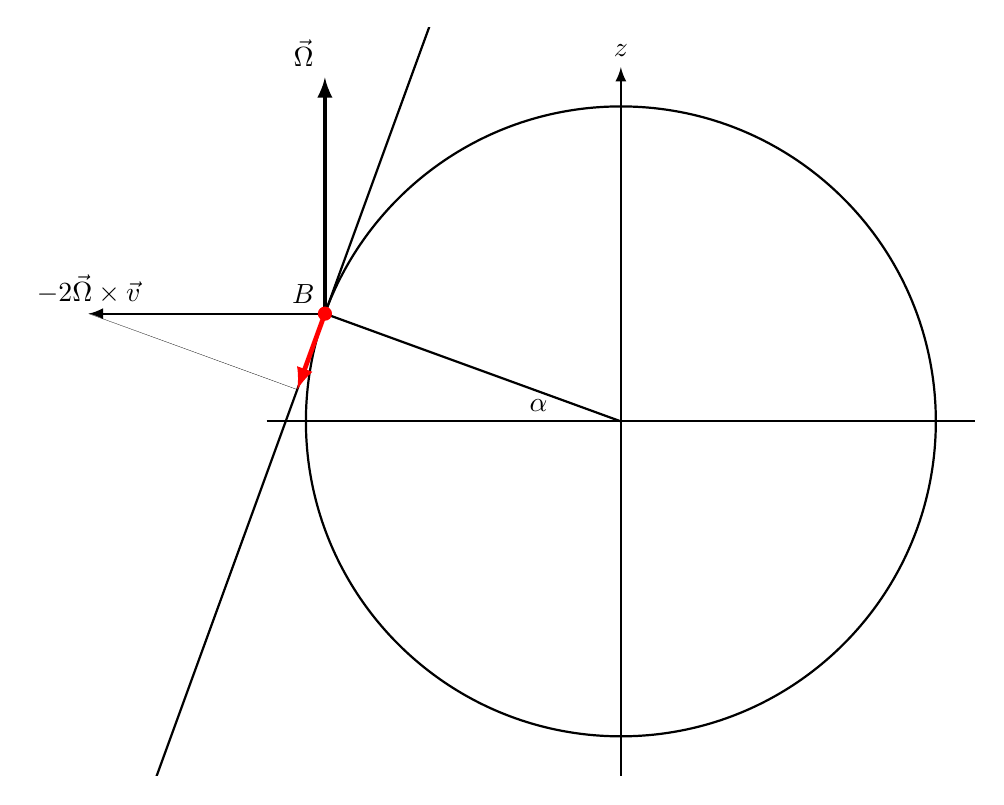
\begin{tikzpicture}[scale=1, >= latex, thick]
\draw[->] (0,-4.5)--(0,4.5) coordinate[label={$z$}];
\draw (0,0) circle[radius=4];
\def\a{70}
\coordinate (B) at ({-4*sin(\a)},{4*cos(\a)});
\node at (B) [above left] {$B$};
\coordinate (C) at ({-4*sin(\a)},{4*cos(\a)+3});
\coordinate (D) at ({-4*sin(\a) - 3},{4*cos(\a)});
\coordinate (E) at ({-4*sin(\a) + 10 * cos(\a)},{4*cos(\a) + 10 * sin(\a)});
\coordinate (F) at ({-4*sin(\a) - 10 * cos(\a)},{4*cos(\a) - 10 * sin(\a)});
\def\l{-3*cos(\a)}
\coordinate (G) at ({-4*sin(\a) + \l*cos(\a)},{4*cos(\a) + \l*sin(\a)});
\draw[line width=0.1] (D)--(G);
\draw (0,0)--(B);
\draw (-4.5,0)--(4.5,0);
\node at (-0.8,0) [above left] {$\alpha$};
\draw[->,line width=1.5pt] (B)--(C) coordinate[label={above left:$\vec{\Omega}$}];
\draw[->] (B)--(D) coordinate[label={above:$-2\vec{\Omega}\times\vec{v}$}];
\begin{scope}
\clip (-7,-4.5) rectangle (4.5,5);
\draw (E)--(F);
\end{scope}
\draw[color=red,line width=1.7pt,->] (B)--(G);
\fill[color=red] (B) circle[radius=0.09];
\end{tikzpicture}
\caption{Berechnung der Coriolis-Beschleunigung für einen
Geschwindigkeitsvektor in $U$-Richtung.
\label{skript:U-coriolis}}
\end{figure}%
Aus Abbildung~\ref{skript:U-coriolis} kann man ablesen,
dass die Komponente der Coriolis-Beschleunigung parallel
zur Tangentialebene $2\omega u\sin(\alpha)$ ist.

Setzen wir die beiden Resultate zusammen finden wir, dass die
Coriolis-Beschleunigung im $U$-$V$-Koordinatensystem
\begin{equation}
\underbrace{
2\omega
\sin\alpha}_{\displaystyle=f}
\begin{pmatrix}
v\\
-u
\end{pmatrix}
\label{skript:physik:coriolis}
\end{equation}
ist.
Die Coriolis-Beschleunigung ist proportional zu $f=2\omega\sin\alpha$, auch
bekannt als der {\em Coriolis-Parameter}.
\index{Coriolis-Parameter}%

\subsubsection{Globale Zirkulation}
Die bisher besprochenen Prinzipien ermöglichen uns, die
global Zirkulation qualitativ zu beschreiben.
Veränderungen der globalen Zirkulation sind langsam,
es ist daher gerechtfertigt, die täglichen Schwankungen der
Einstrahlung infolge der Erdrotation durch eine mittlere
Einstrahlung zu ersetzen.
Die Bedingungen für die globale Zirkulation sind daher rotationssymmetrisch
um die Erdachse.
Wir suchen daher nach einem globalen Strömungsmuster, welches ebenfalls
rotationssymmetrisch ist.

\begin{figure}
\centering
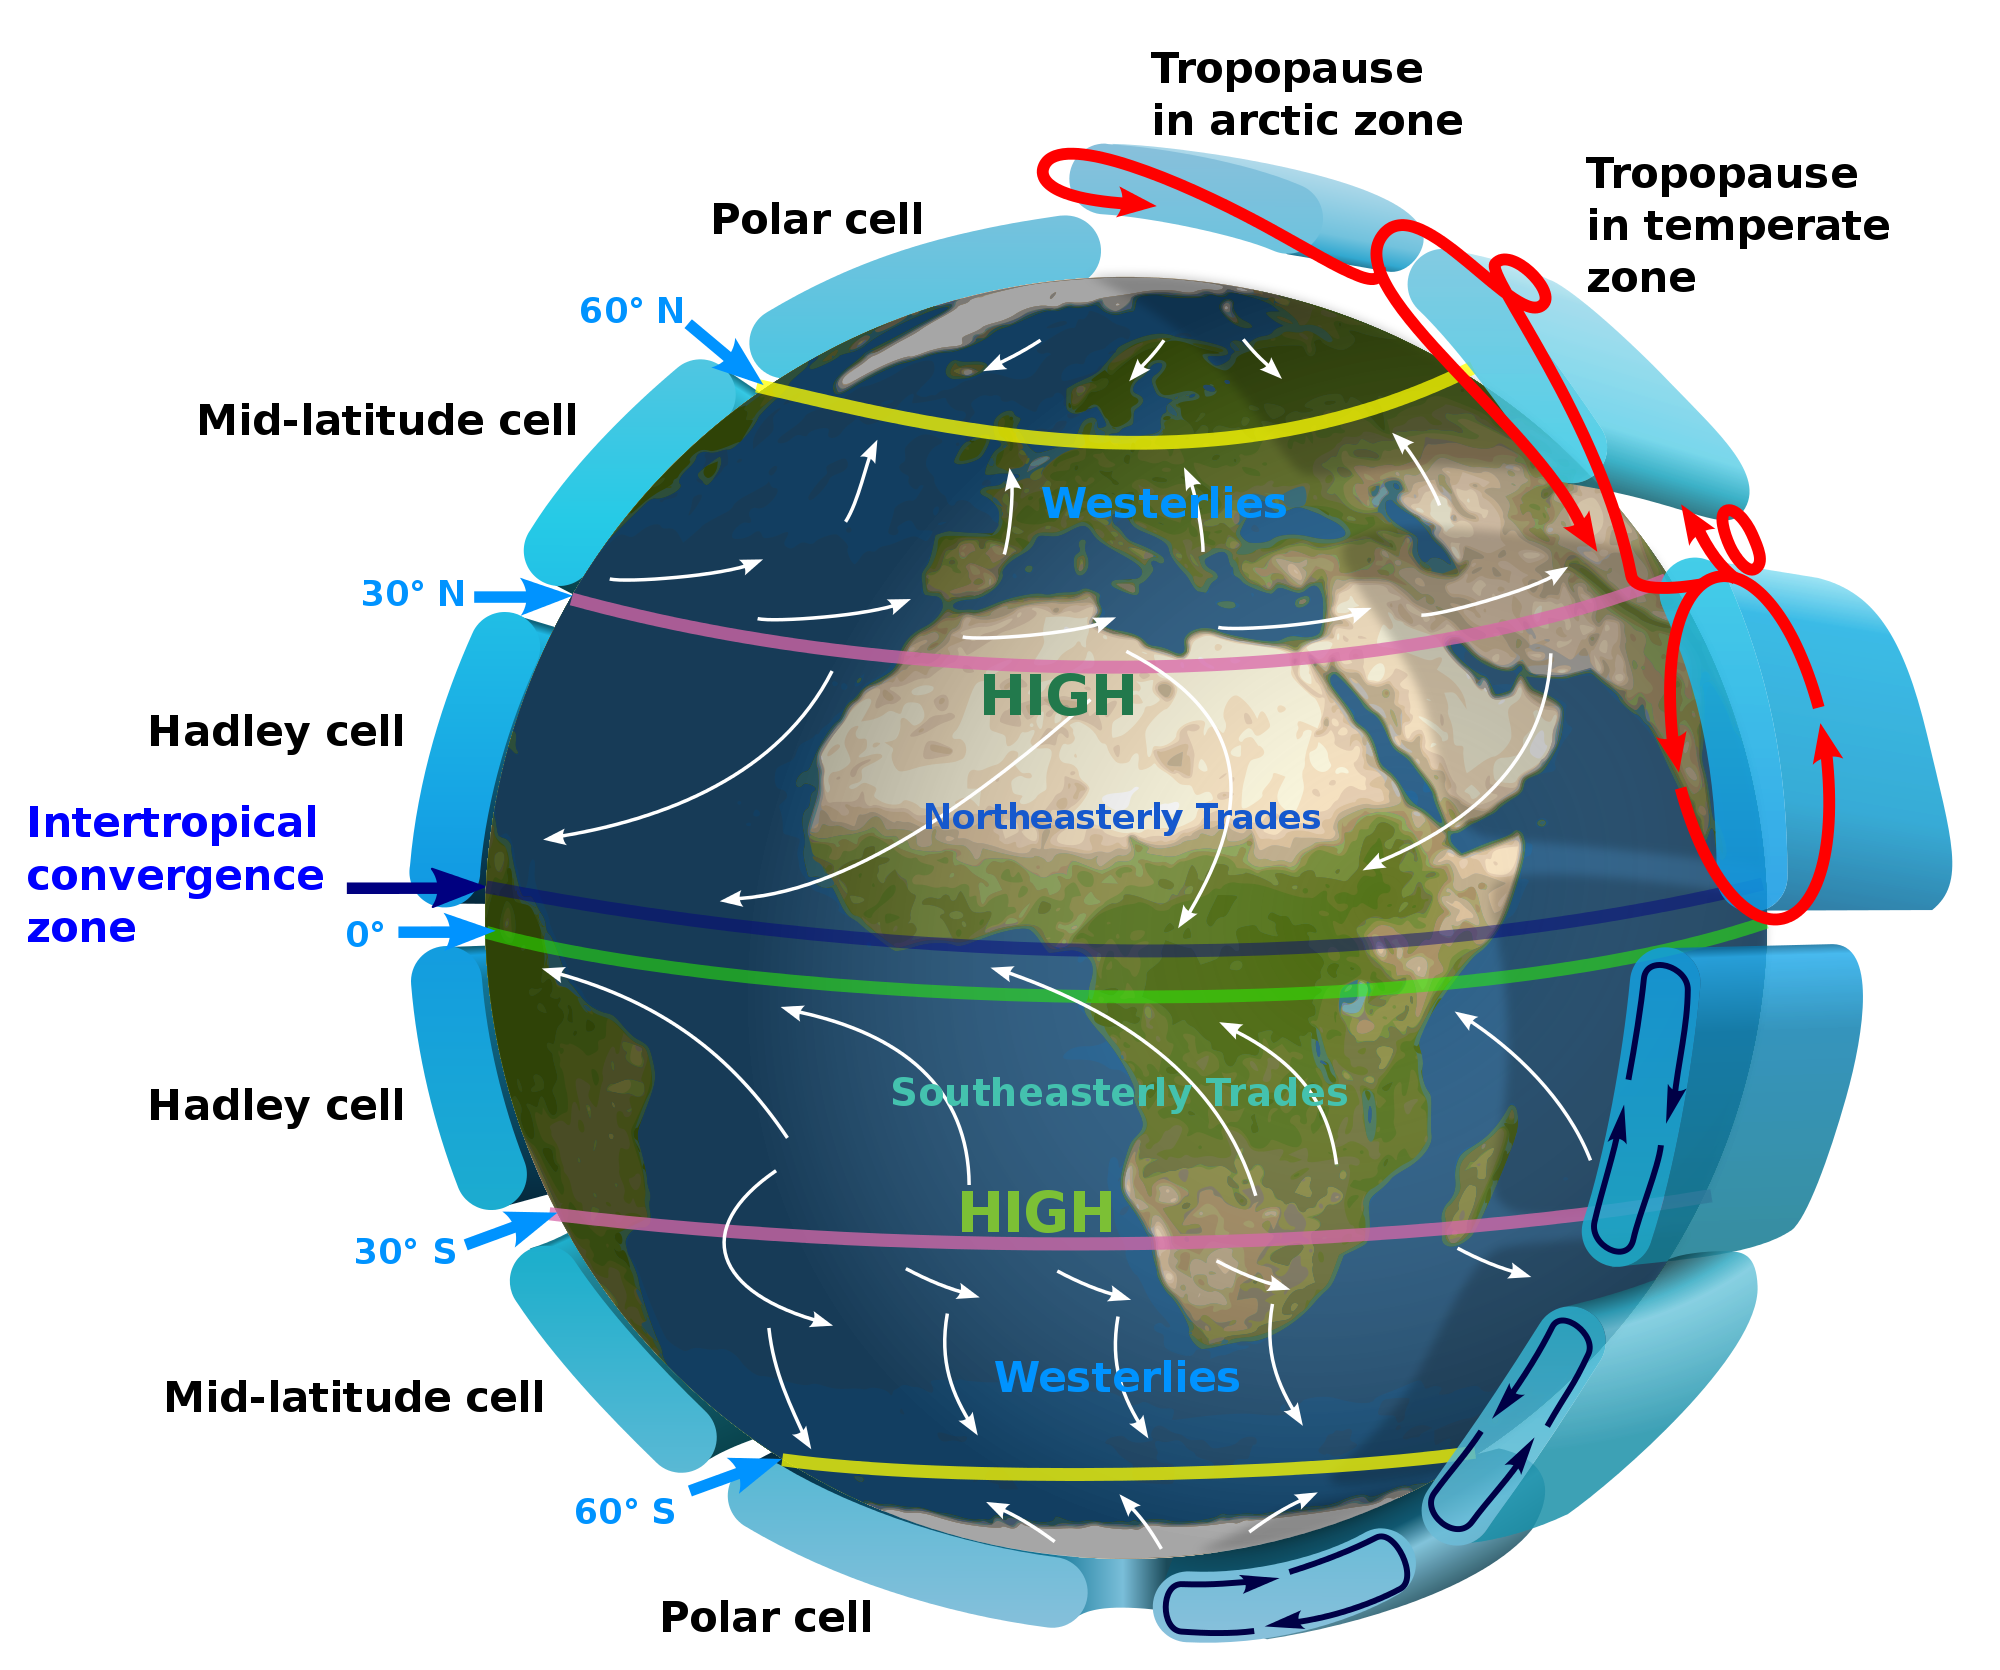
\includegraphics[width=\hsize]{chapters/1/Earth_Global_Circulation_-_en.png}
\caption{Globale Zirkulation der Erde
\label{skript:globalezirkulation}}
\end{figure}

Die grösste Einstrahlung erfolgt am Äquator, erwärmt die Luft und
lässt sie aufsteigen.
Der entstehenden Unterdruck in Äquatornähe erzeugt eine 
Ausgleichsströmung in Bodennähe.
Die aufsteigende Luft kann nicht beliebig hoch aufsteigen und weicht
daher in grosser Höhe in Richtung der Pole aus.
Die Höhenströmung nach Norden wird von der Coriolis-Beschleunigung nach
rechts abgelenkt, sie kann also nicht beliebig weit nach Norden
strömen, bevor sie wieder absinkt.
Es entsteht je eine geschlossene Konvektionszelle wie in
Abbildung~\ref{skript:globalezirkulation}, die sogenannte
Hadley-Zelle \cite{skript:hadley}.

Im Anschluss an die Hadley-Zellen entstehen auf Grund des gleichen
Mechanismus weitere Zellen.
Die Breite der Zellen hängt offenbar von der Stärke des Coriolis-Effektes ab.
Auf einem Planeten mit grösserer Rotationsgeschwindigkeit erwartet man
vergleichsweise schmalere Zellen.
\begin{figure}
\centering
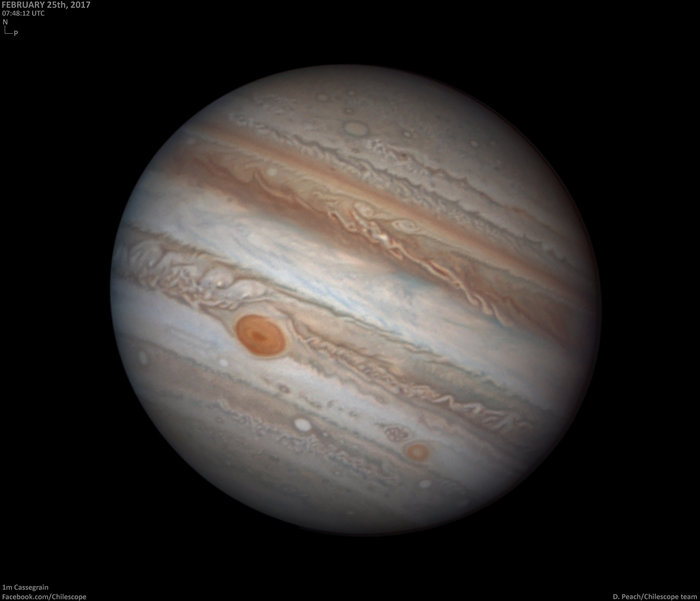
\includegraphics[width=\hsize]{chapters/1/Jupiter_on_25_February_2017_node_full_image_2.jpg}
\caption{Jupiter mit Wolkenbändern, Aufnahme von Damian Peach
\cite{skript:jupiter}
\label{skript:jupiterzirkulation}}
\end{figure}
Dies ist genau was man am Beispiel der globalen Strömung auf dem
Jupiter in Abbildung~\ref{skript:jupiterzirkulation} beobachten kann.

\subsubsection{Äquatorialzone}
Nahe dem Äquator ist die geographische Breite $\alpha$ klein und
damit auch der Coriolis-Parameter $f$.
Die Strömung in Äquatornähe ist daher praktisch unbeeinflusst 
vom Coriolis-Effekt.
Entlang des Äquators kann die Luft oder das Meer also
unbeeinflusst durch die Coriolis-Beschleunigung strömen.

Mit Hilfe der $\beta$-Ebene können wir jetzt aber auch modellhaft 
die Bewegung eines Massepunktes in Äquatornähe berechnen.
Wenn die Coriolis-Beschleunigung der einzige Einfluss ist, dann
\begin{equation}
\frac{d}{dt}
\begin{pmatrix}u\\v\end{pmatrix}
=
f\begin{pmatrix}v\\-u\end{pmatrix}.
\end{equation}
Der Coriolis-Parameter $f=2\omega\sin\alpha$ ist proportional
zur geographischen Breite.
Für nicht zu grosse geographische Breiten können wir $\sin\alpha$ durch
die $y$-Koordinate erstzen.
Wir müssen also die Differentialgleichung
\begin{equation}
\frac{d}{dt}
\begin{pmatrix}x\\y\\u\\v\end{pmatrix}
=
\begin{pmatrix}
u\\v\\fyv\\-fyu
\end{pmatrix}.
\label{skript:coriolis-dgl}
\end{equation}
lösen.
Die Gestalt der Lösungskurven hängt von der Anfangsgeschwindigkeit und
vom Parameter $f$ ab.
Für $f=0$ fällt die Coriolis-Beschleunigung ganz weg, in diesem
Fall sind die Lösungskurven Geraden.

\begin{figure}
\centering
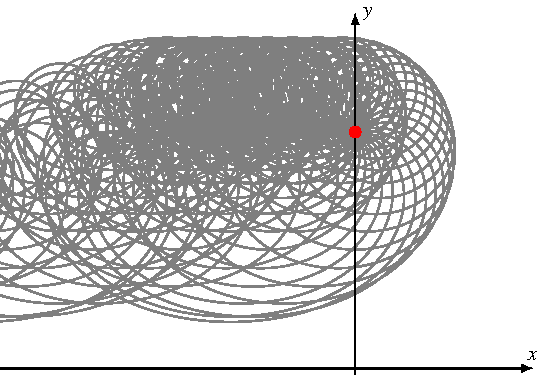
\includegraphics{chapters/1/stream.pdf}
\caption{
Lösungen der Differentialgleichung ausgehend vom Punkt $(0,4)$
mit Anfangsgeschwindigkeit $|\vec{v}|=1$ und $f=0.26$.
Die Bahnkurven sind immer nach rechts gekrümmt und bleiben in der
oberen Halbebene.
\label{skript:stream-graph}}
\end{figure}

\begin{figure}
\centering
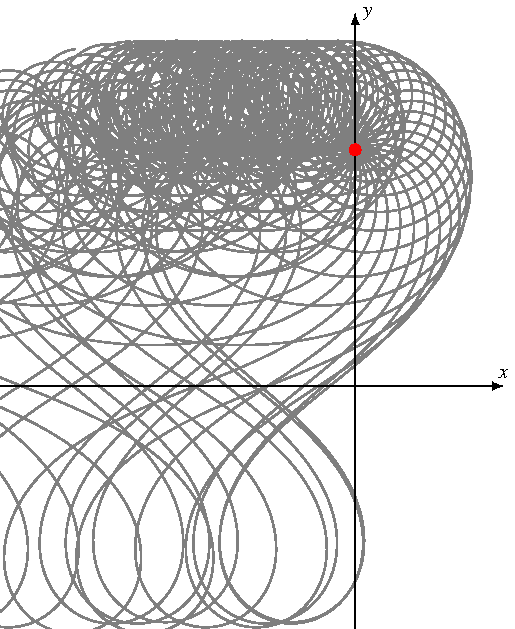
\includegraphics{chapters/1/cross.pdf}
\caption{
Lösungen der Differentialgleichung ausgehend vom Punkt $(0,4)$
mit Anfangsgeschwindigkeit $|\vec{v}|=1$ und $f=0.22$.
Einzelne Bahnkurven kreuzen die $x$-Achse und krümmen sich in der unteren
Halbeben dann links.
\label{skript:cross-graph}}
\end{figure}

Um einen Überblick über die möglichen Lösungskurven zu erhalten, berechnen
wir numerisch die vom Punkt $(0,4)$ ausgehenden Lösungskurven 
der Differentialgleichung~\ref{skript:coriolis-dgl}.
Je grösser $f$ ist, desto stärker gekrümmt sind die Lösungskurven.
Solange die Kurven in der oberen Halbebene $y>0$ liegen sind die Kurven
nach rechts gekrümmt.
Für genügend grosses $f$ bleiben alle Kurven in der oberen
Halbebene wie in Abbildung~\ref{skript:stream-graph}, unabhängig
von der Richtung der Anfangsgeschwindigkeit.
Für kleinere Werte von $f$ wie in Abbildung~\ref{skript:cross-graph}
gelangen einzelne Bahnkurven in die untere Halbebene wo die Krümmung
der Kurve von rechts auf links kehrt.

Man beachte, dass diese Bahnkurven nicht Stromlinien einer Strömung sind,
da sich diese nicht kreuzen können.
Dieses einfache Modell ist also nicht geeignet, die tatsächliche Bewegung
der Luftmassen darzustellen, dazu müssen wir die Gleichungen
der Fluiddynamik in Kapitel~\ref{chapter:fluiddynamik}.

\subsubsection{Meeresströmungen}
Meeresströmungen leisten einen bedeutenden Beitrag zum Klima, weil sie
dank der hohen Wärmekapazität von Wasser auch bei kleiner
Strömungsgeschwindigkeit und sehr viel kleinerem bewegtem Volumen als
bei den atmosphärischen Strömungen eine grosse Energiemenge transportieren
können.

\subsection{Periodische Einflüsse}
Das Klimasystem ist einer Reihe von sich periodisch verändernden 
Einflüssen ausgesetzt.
Viele dieser Einflüsse erscheinen auf den ersten Blick geringfügig
und damit vernachlässigbar.
Doch wenn ein solcher periodischer Einfluss mit einer Frequenz auftritt,
der einer Eigenfrequenz des Klimasystems entspricht, dann kann sich 
in Folge eines Resonanzeffektes über längere Zeit ein bedeutender 
Einfluss auf das Klima manifestieren.
Es ist daher wichtig, auch kleine Einflüsse zu kennen und insbesondere
alle Aspekte des Klimasystems zu modellieren, die eine Eigenfrequenz
in der Nähe ihrer Anregungsfrequenzen haben.

\subsubsection{Sonnenfleckenzyklus}
\index{Sonnenflecken}%
\index{Sonnenfleckenzyklus}%
Die Strahlung der Sonne ist nicht konstant.
Wie bei jedem Stern dieser Klasse nehmen Durchmesser und Temperatur der
Sonne über die Jahrmillionen in dem Mass zu, dass neben der Fusion
von Wasserstoff zu Helium auch noch Fusionsprozesse schwerer Elemente
eine Rolle zu spielen beginnen.
Dieser sehr langfristige Einfluss ist jedoch nur wesentlich für
den Vergleich von Klimamodellen mit Daten über das Klima auf der sehr
jungen Erde.

Für kurzfristige Prognosen von Bedeutung sind dagegen die Schwankungen
der Sonnenaktivität.
\index{Sonnenaktivität}%
Die Zahl der Sonnenflecken ist ein leicht zu messender Indikator
dafür, für den Aufzeichnung seit dem 17.~Jahrhundert existieren.
Die Sonnenfleckenzahl schwankt mit einer Periode von etwa elf Jahren.
Die daraus resultierende Änderung der Einstrahlung ist jedoch nur 0.07\%,
so dass die Sonnenaktivität nicht für den Klimawandel verantwortlich
gemacht werden kann. 
Die schwankende Sonnenaktivität muss jedoch bei der Validierung
von Klimamodellen berücksichtigt werden.

\subsubsection{Bahnänderungen der Erde}
\index{Bahnänderungen}%
Nach Kepler bewegen sich die Planeten auf Ellipsen,
in deren einem Brennpunkt die Sonne steht.
Die keplerschen Gesetze der Planetenbahnen können aus dem Newtonschen 
Gravitationsgesetz hergeleitet werden
\cite[\S 6]{skript:joos}.
\index{Bahnelemente}%
\index{Keplersche Gesetze}%
Die Bahnelemente beschreiben die Ebene, in der sich der Planet bewegt,
die Richtung und der Zeitpunkt der grössten Annäherung an die Sonne und
die Exzentrizität der Ellipse.
\index{Exzentrizität}%
%
Es trifft exakt jedoch nur dann zu, wenn keine anderen Kräfte auf den
Planeten wirken als die Anziehungskraft der Sonne.
Newtons Gravitationsgesetz besagt nämlich, dass auch alle anderen
\index{Gravitationsgesetz}%
Planeten durch ihre Schwerkraft auf die Erde einwirken.
Dies äussert sich darin, dass sich die Bahnelemente mit der Zeit
ändern.
Diese langsame Veränderung der Bahnelemente war schon Newton bekannt,
er hat daraus geschlossen, dass das Sonnensystem mit der Zeit völlig
zerfallen würde.
Genauere Untersuchungen und numerische Rechnungen zeigen jedoch, dass
unser Sonnensystem über lange Zeit stabil ist.
Die Exzentrizität zum Beispiel der Erdbahn kann sich tatsächlich verändern,
aber über längere Zeit wird die Veränderung auch wieder rückgängig
gemacht.

Veränderungen der Erdbahn, insbesondere der Exzentrizität, oder der
Neigung der Erdachse zur Bahn äussern sich darin, dass die Einstrahlung
über das Jahr stärker oder weniger stark schwankt oder auch im Mittel
grösser oder kleiner wird.
\index{Neigung der Erdachse}%
Dadurch können sich die Temperaturunterschiede zwischen den Polgebieten und
äquatorialen Breiten verändern und damit die Intensität des Wettergeschehens
beeinflusst werden.
Ein langfristiges Klimamodell muss also auch diese Änderungen
modellieren.

Es stellt sich allerdings heraus, dass diese Veränderungen sehr viel
langfristiger sind als der die meisten Klimapolitiker interessierenden
Zeitraum von wenigen Jahrhunderten.
Die Berücksichtigung dieser Effekte dient daher vor allem dazu die
Klima-Modelle mit der Klimageschichte der Erde zu vergleichung und
damit zu validieren.
In Kapitel~\ref{chapter:fourier} wird gezeigt, wie periodische Einflüsse
modelliert und mit Hilfe der Fourier-Theorie analysiert werden können.
Und in Kapitel~\ref{chapter:neigung} wird gezeigt, wie die periodischen
Störungen der Erdbahnneigung zu dramatischen Veränderungen des Klimas
führen können.






%
% anforderungen.tex -- Anforderungen an Klima-Modelle
%
% (c) 2018 Prof Dr Andreas Müller, Hochschule Rapperswil
%

\section{Anforderungen an Klima-Modelle\label{section:anforderungen}}
Aus der vorangegangenen Diskussion können wir einige Anforderungen
ableiten, was Klimamodelle können müssen, was sie berücksichten
müssen und welche Aspekte sie vernachlässigen können.

Das Ziel ist die Modellierung der Klima-Entwicklung über wenige
hundert Jahre.
Es ist jedoch nicht erforderlich, den vollständigen Zustand der
Atmosphäre von Tag zu Tag zu modellieren.
Es genügt diejenigen Eigenschaften zu modellieren, die 
für den Energiehaushalt der Erde wesentlich sind.
Dazu gehören die folgenden Eigenschaften.
\begin{enumerate}
\item
Der Strahlungshaushalt der Erde muss korrekt modelliert werden,
da dies die global Mitteltemperatur bestimmt.
Dies bedeutet insbesondere auch, dass die Albedo sowie der Gehalt an
Treibhausgasen korrekt wiedergeben werden.
\item
Die Albedo der Erde muss modelliert sein. 
D.~h.~der durchschnittliche Vereisungsgrad und die Häufigkeit und
Dichte von Bewölkung muss korrekt wiedergeben sein.
\item
Strahlungs- und Wasserhaushalt der Atmosphäre unterscheiden sich
über Kontinenten und über den Ozeanen.
Das Modell muss daher räumlich genügend aufgelöst sein, dass die
für den Energiehaushalt wesentlichen Unterschiede abgebildet
werden können.
\item
Die Energietransportmechanismen müssen für Zeitskalen in der Grössenordnung
von Jahren und Jahrzehnten korrekt modelliert sein, weil dies die
Verteilung der Energie über die Erdoberfläche festlegt.
\item
Wasser in der Atmosphäre hat einerseits einen grossen Einfluss auf
den Treibhauseffekt, übernimmt aber auch für einen wesentlichen Teil
des Energietransports in der Atmosphäre.
Daher muss der Wassergehalt 
\item
Der Salzgehalt der Meere treibt die thermohaline Zirkulation an, welche
auf einer Zeitskala von Jahrzehnten einen wesentlichen Beitrag zum
Energietransport in den Ozeanen leistet.
Salzgehalt und Verdunstung an der Meeresoberfläche muss so genau
modelliert sein, dass diese Energieströme korrekt modelliert werden.
\end{enumerate}

Um die Auswirkungen des Klimawandels zu verstehen muss man vorhersagen,
wie sich kurzfristige Wetterphänomene verändern.
Dazu kann man gewöhnliche Wettermodelle verwenden, die sowohl zeitlich wie
auch räumlich eine bessere Auflösung haben.
Man kann aber gewisse qualitative Aussagen auch ohne solche detaillierten
Modelle machen.
Ein höherer Wassergehalt der Atmosphäre wird zum Beispiel zunächst
zu stärkeren Niederschlägen führen.
Da aber auch mehr Energie in Form von latenter Wärme zur Verfügung
steht, muss man auch mit stärkeren Winden rechnen.
Zum Beispiel muss man also damit rechnen, dass Hurrikane intensiver
werden.

\subsection{Validierung von Klimamodellen}
Wie können wir überprüfen, ob wir die wesentlichen Einflussfaktoren
auf das Klimasystem und ihre Auswirkungen verstanden haben?
Warum sollen wir den Prognosen der Klimamodelle überhaupt glauben?
Wir können ja nicht wie bei einem Laborexperiment ein paar Parameter
verändern, nachmessen, wie das System sich verändert, und überprüfen,
ob die Änderungen mit den Vorhersagen des Modells übereinstimmen.

\subsubsection{Vergleich mit anderen Planeten}
Im Sonnensystem stehen uns die sechs Planeten Venus,
Mars, Jupiter, Saturn, Uranus und Neptun mit einer Atmosphäre und
der Saturnmond zur Verfügung, um Klimamodelle damit zu überprüfen.
Die Verhältnisse auf diesen Planeten sind zwar zum Teil extrem verschieden
von der Situation auf der Erde.
Die grundlegenden physikalischen Prozesse sind jedoch die selben.
Die Modelle, die wir für die Erde entwickeln, sollten daher auch
die Situation auf diesen Planeten wiedergeben können.
Tun sie dies nicht, ist dies in Indiz dafür, dass uns ein wesentlicher 
Klimafaktor entgangen ist, der zum Beispiel in der zukünftigen Klimaentwicklung
eine Rolle spielen könnte.

Als Beispiel betrachten wir den Planeten Venus.
Die Venus ist etwa gleich gross wie die Sonne, ist aber von Wolken
bedeckt und hat daher eine wesentlich höhere Albedo.
Die mittleren Entfernungen von Venus und Erde zur Sonne verhalten
sich wie
\[
a_{\venus}
:
a_{\earth}
=
0.72,
\]
die Solarkonstante für die Venus ist also 1.92 mal grösser.
Nach dem Stefan-Boltzmannschen Gesetz müsste die Venus im Vergleich
zur Erde nur etwa 17\% wärmer sein, um die im visuellen Bereich
absorbiert Energie im infraroten wieder abzustrahlen.
Wir würden also eine Temperatur von $1.17\cdot 287\text{K})=336\text{K}$
erwarten.
Die tatsächlich Oberflächentemperatur ist mit $737\,\text{K}$ jedoch viel
höher.
Daran kann man bereits erkennen, dass die Venus einen wesentlich
stärkeren Treibhauseffekt haben muss, der nach einer Erklärung
verlangt.

Andererseits hat der Planet Mars eine 1.52mal grössere mittlere
Entfernung und damit ist die Einstrahlung dort nur 43\% von der
Einstrahlung auf der Erde.
Wieder nach dem Stefan-Boltzmann-Gesetz würde dies verlangen, dass die
Temperatur etwa 80\% der Temperatur der Erde betragen müsste,
also etwa $0.8\cdot 287\text{K} = 224.9\text{K}$, was recht genau
der beobachteten Temperatur von $218\text{K}$ entspricht.
Der Treibhauseffekt ist auf dem Mars also wesentlich geringer, was
vor allem auf die sehr viel dünnere Atmosphäre zurückzuführen ist.

Tatsächlich besteht die Venusatmoshpäre zu 96\% aus Kohlendioxid und
hat eine sehr viel höhere Dichte, was den intensiveren Treibhauseffekt
erklären kann.

\subsubsection{Vergleich mit der Vergangenheit}
Die Erdatmosphäre hat sich im Laufe der Erdgeschichte stark verändert.
Die jüngere Geschichte kann zum Beispiel aus Bohrkernen aus antarktischem
Eis rekonstruiert werden.
Für die Frühgeschichte der Erdatmosphäre gibt es keine solchen direkten
Messungen.

Die chemischen Verwitterungsprozesse hängen jedoch von der chemischen
Zusammensetzung und Temperatur der Atmosphäre ab.
Aus der beobachteten Zusammensetzung von Verwitterungsprodukten und
Sedimenten kann man also Rückschlüsse darauf ziehen, was für Verhältnis
im Zeitpunkt der Entstehung dieser Sedimente vorgeherrscht haben müssen.

\subsection{Klimageschichte der Erde}




%\section{Klima}
%\rhead{Klima}
%In der Wikipedia kann man die folgenden Definitionen für die Begriffe Wetter
%und Klima finden:
%
%\begin{definition}
%Als {\em Wetter} bezeichnet man den
%spürbaren, kurzfristigen Zustand der Atmosphäre (auch: messbarer
%Zustand der Troposphäre) an einem bestimmten Ort der Erdoberfläche,
%der unter anderem als Sonnenschein, Bewölkung, Regen, Wind, Hitze
%oder Kälte in Erscheinung tritt.
%\cite{skript:wetter}
%\end{definition}
%
%\begin{definition}
%Das {\em Klima} steht als Begriff für die Gesamtheit aller meteorologischen
%Vorgänge, die für die über Zeiträume von mindestens 30 Jahren
%regelmässig wiederkehrenden durchschnittlichen Zustände der Erdatmosphäre
%an einem Ort verantwortlich sind.
%\cite{skript:klima}
%\end{definition}
%
%Was also Donald Trump in seinem Tweet beschrieben hat ist das Wetter.
%Selbst wenn die Temperatur in New York unter den Gefrierpunkt fällt, 
%heisst das nicht, dass die mittlere Temperatur in New York über mehrere
%Jahre nicht doch ansteigen kann.
%Tatsächlich bedeutet ``globale Erwärmung'' nicht, dass die mittlere
%Temperatur an jedem Punkt der Erde zunehmen wird.
%Im Gegenteil ist es durchaus möglich, dass zwar die mittlere Temperatur
%der Erde ständig zunimmt, wie wir in den letzten Jahren auch messtechnisch
%nachweisen konnten, dass aber auch die Temperaturunterschiede stark zunehmen,
%so dass es am Ende an einzelnen Stelle der Erdoberfläche zu einer 
%Abkühlung kommen kann.
%Um dieser Komplexität Rechnung zu tragen, spricht man nicht mehr von
%der ``globalen Erwärmung'', sondern vom Klimawandel.
%
%Auch wenn das Wetter nur sehr eingeschränkt vorhersagen lässt,
%bedeutet das noch lange nicht, dass das Klima nicht doch sehr
%genau vorhergesagt werden kann.
%Eine Analogie kann den Unterschied zwischen der Vorhersagbarkeit
%von Wetter und Klima verdeutlichen.
%Wenn man in einem Kochtopf Wasser zum Kochen bringt, stellt sich
%eine unverrhersagbare chaotische Bewegung kleiner und grosser
%Gasblasen ein.
%Es ist unmöglich vorherzusagen, wann und wo sich die nächste Blase
%bilden wird und welchen Weg sie an die Oberfläche des Wasser nehmen
%wird.
%Wenn wir aber nur die mittlere Temperatur betrachten, können wir
%aus der Heizleistung der Kochplatte, der Masse und der spezifischen
%Wärmekapazität des Wassers genau berechnen, welche Temperatur zu welcher
%Zeit im Wasser herschen wird und wir können den Zeitpunkt exakt
%vorhersagen, wann das Wasser zu sieden beginnt.
%Die mittlere Temperatur des Wassers beschreibt das ``Klima''
%in der Pfanne, die kleinräumigen und kurzfristigen Blasen und anderen
%Turbulenzen beschreiben das ``Wetter''.
%
%\section{Physikalische Eigenschaften des Klimasystems}
%In diesem Abschnitt stellen wir die physikalischen Eigenschaften
%aller wesentlicher Komponenten des Klimasystems zusammen.
%Dabei geht es zunächst nur darum, die grundlegende Physik in 
%Erinnerung zu rufen und die Naturgesetze, die die Wechselwirkungen
%zwischen den Komponenten beschreiben.
%Auf die Details der mathematischen Modellierung der zukünftigen
%Veränderung dieser Grössen werden wir erst später eingehen.
%
%\subsection{Wärme, Konvektion, Kondensation}
%Die wohl wichtigste Klima-Grösse ist die Temperatur.
%Sie drückt aus, wieviel Energie in Form von Wärme ein Körper enthält.
%
%\subsubsection{Wärmekapazität}
%Die spezifische Wärme $C$ gibt an, wie die innere Energie sich bei
%einer Temperaturänderung $\Delta T$ verändert:
%\[
%\Delta E = C\cdot\Delta T.
%\]
%Der Körper speichert Energie in Form der thermischen Bewegung der
%einzelnen Atome.
%Schwerere Atome können bei gleicher Bewegungsgeschwindigkeit 
%mehr Energie speichern.
%Stoffe mit grösserer Dichte können mehr Atome und damit auch mehr
%Wärmeenergie in einem kleineren Volumen unterbringen.
%Die spezifische Wärmekapazität $c$ gibt an, welche Wärmekapazität
%ein Kilogramm eines Stoffes hat.
%Ein Körper der Masse $m$ hat also die Wärmekapazität $C=cm$.
%
%\subsubsection{Wärmeleitung}
%Herrschen in einem Körper Temperaturunterschiede, ist $T$ nicht mehr
%nur eine konstante, sondern eine Funktion der Koordinaten und auch der
%Zeit.
%Temperaturunterschiede werden sich ausgleichen, indem Energie von
%wärmeren zu kälteren Teilen des Körpers fliegt.
%Dies geschieht umso schneller, je grösser die Unterschiede sind.
%Die Wärmeleitungsgleichung
%\begin{equation}
%\frac{\partial T}{\partial t}
%=
%\kappa
%\biggl(
%\frac{\partial^2}{\partial x^2}
%+
%\frac{\partial^2}{\partial y^2}
%+
%\frac{\partial^2}{\partial z^2}
%\biggr)
%T
%\label{skript:waermeleitung}
%\end{equation}
%beschreibt die Entwicklung der Funktion $T(x,y,z,t)$ an jedem
%Ort des Raumes \cite{skript:waermeleitung}.
%Der Koeffizient $\kappa$ ist eine Materialkonstante, die beschreibt,
%wie schnell sich die Temperaturunterschiede ausgleichen können.
%Ist $\kappa=0$, folgt $\partial T/\partial t=0$, die Temperatur 
%ändert sich nicht, es findet keine Wärmeleitung statt.
%
%Die rechte Seite von \eqref{skript:waermeleitung} kann mit dem
%sogenannten Laplace-Operator gemäss der folgenden Definition 
%geschrieben werden.
%
%\begin{definition}
%Der Operator
%\[
%\Delta
%=
%\frac{\partial^2}{\partial x^2}
%+
%\frac{\partial^2}{\partial y^2}
%+
%\frac{\partial^2}{\partial z^2}
%\]
%heisst der
%{\em Laplace-Operator}.
%\end{definition}
%
%Die Wärmeleitungsgleichung erhält damit die Form
%\begin{equation}
%\frac{\partial T}{\partial t}
%=
%\kappa\Delta T.
%\label{skript:waermeleitung2}
%\end{equation}
%
%\subsubsection{Konvektion}
%Wärmeleitung kann Wärmeenergie nur vergleichsweise langsam transportieren.
%Das einleitende Beispiel des Kochtopfs zeigt auch, wie ein effizienterer
%Energietransport funktionieren kann.
%In der Atmosphäre dehnt sich warme Luft aus.
%Dank der geringeren Dichte können warme Luftblasen aufsteigen und damit
%Wärme viel effizienter in die obere Atmosphäre transportieren
%als dies mit Wärmeleitung möglich wäre.
%Dieser Prozess heisst {\em Konvektion} \cite{skript:konvektion}.
%\index{Konvektion}%
%
%Wir wollen den Fall eines strömenden Mediums mathematisch etwas genauer
%ausarbeiten.
%Bewegt sich das Medium mit der Geschwindigkeit $\vec v$, dann ändert sich
%die Temperatur des Mediums, welches sich über dem Punkt $P=(x,y,z)$
%befindet.
%Nach der Zeit $\Delta t$ befindet sich derjenige Teil des Mediums
%über dem Punkt $P$, der sich vorher über dem Punkt $P-\Delta t\cdot\vec v$
%befand.
%Die Temperatur zur Zeit $t+\Delta t$ ist daher
%$T(P,t+\Delta t)=T(P-\Delta t,t)$.
%Die Temperaturänderung
%\begin{align*}
%T(P,t+\Delta t)
%&=
%T(P,t) + (T(P,t+\Delta t)-T(P,t))
%=
%T(P,t) + T(P-\vec v\Delta t, t)-T(P,t)
%\\
%\frac{
%T(P,t+\Delta t)
%-
%T(P,t)
%}{\Delta t}
%&=
%\frac{
%T(P-\vec v\Delta t, t)-T(P,t)
%}{\Delta t}.
%\end{align*}
%Beim Grenzübergang $\Delta t\to 0$ wird aus der linken Seite die
%partielle Ableitung nach $t$.
%Die rechte Seite kann mit Hilfe der Kettenregel berechnet weren.
%Es wird
%\begin{equation}
%\frac{\partial T}{\partial t}
%=
%-
%\frac{\partial T}{\partial x} v_x
%-
%\frac{\partial T}{\partial y} v_y
%-
%\frac{\partial T}{\partial z} v_z.
%\label{skript:advektion1}
%\end{equation}
%Der Ausdruck auf der rechten Seite kann vektoriell mit der folgenden
%Definition etwas eleganter geschrieben werden.
%
%\begin{definition}
%Der vektorielle Operator 
%\[
%\nabla
%=
%\begin{pmatrix}
%\frac{\partial}{\partial x}\\
%\frac{\partial}{\partial y}\\
%\frac{\partial}{\partial z}
%\end{pmatrix}
%\]
%heisst der {\em Nabla-Operator}.
%Der Vektor
%\[
%\nabla f
%=
%\begin{pmatrix}
%\frac{\partial f}{\partial x}\\
%\frac{\partial f}{\partial y}\\
%\frac{\partial f}{\partial z}
%\end{pmatrix}
%=
%\operatorname{grad} f
%\]
%heisst der {\em Gradient} von $f$.
%\end{definition}
%\index{Gradient}%
%\index{Nabla-Operator}%
%
%Die Temperaturänderung in Folge der Strämung 
%\eqref{skript:advektion1}
%wird 
%\begin{equation}
%\frac{\partial T}{\partial t}
%=
%-\vec{v}\cdot\nabla T.
%\label{skript:advektion2}
%\end{equation}
%\index{Advektion}%
%Man nennt diese Temperaturänderung durch die Strömung auch
%{\em Advektion}.
%Die Wärmeleitungsgleichung kann damit zu einem umfassenderen
%Modell
%\begin{equation}
%\frac{\partial T}{\partial t}
%=
%-\vec{v}\cdot\nabla T +\kappa\Delta T
%\label{skript:waermeleitungadvektion}
%\end{equation}
%zusammengefasst werden.
%Es ist geeignet für die Beschreibung sowohl der Atmosphäre wie auch des
%Wärmeaustausches in den Ozeanen.
%
%\subsubsection{Phasenübergänge}
%
%\subsection{Strahlung}
%
%\subsection{Erdrotation und Zirkulation}
%
%\subsection{Periodische Einflüsse}
%
%\section{Anforderungen an Klima-Modelle}
%
%
%
		% 1
%
% dgl.tex
%
% (c) 2018 Prof Dr Andreas Müller, Hochschule Rapperswil
%
\section{Grundlagen}
\rhead{Grundlagen}
Eine Differentialgleichung ist eine Beziehung zwischen einer Funktion und
ihren Ableitungen.
Wir betrachten Funktionen der Zeit $t$ mit Werten in $\mathbb R^n$
und schreiben sie $x(t)$.
Sei $f$ eine Funktion
\[
f\colon \mathbb R^n\times \mathbb R \to \mathbb R^n: (x,t) \mapsto f(x,t).
\]

\begin{definition}
Eine Funktion $x(t)$ heisst Lösung der Differentialgleichung
\begin{equation}
\frac{dx}{dt} = f(x,t)
\label{skript:dgl:dgldef}
\end{equation}
zur Anfangsbedingung $x_0$, wenn gilt $x(0)=x_0$ und
\[
\frac{dx(t)}{dt} = f(x(t),t)
\]
für alle $t>0$.
\end{definition}

Unter einigermassen milden Bedingungen an die Funktion $f(x,t)$ ist
sichergestellt, dass eine Differentialgleichung immer eine Lösung hat.

\subsection{Autonome Differentialgleichungen}
Wenn die Funktion $f$ von der Zeit abhängt, wird es im allgemeinen
keine konstanten Lösungen geben.
Für die Klimadiskussion sind wir allerdings daran interessiert, ob
ein Modell Lösungen hat, die sich mit der Zeit nicht ändern.
Solche Lösungen zeigen uns, dass wir alle kurzfristigen
Schwankungen, die wir dem Wetter zuordnen würden, ausgemittelt haben.

\begin{definition}
Eine Differentialgleichung der Form~\eqref{skript:dgl:dgldef}
heisst {\em autonom},
\index{autonom}%
wenn die Funktion $f$ nicht von der Zeit abhängt.
Eine autonome Differentialgleichung kann als
\[
\frac{dx}{dt} = f(x)
\]
geschrieben werden.
\end{definition}

\subsection{Umwandlung in eine autonome Differentialgleichung}
Die Forderung, dass die Differentialgleichung autonom sein soll, ist
auf triviale Art erfüllbar, indem man zu einer neuen
unabhängigen Variablen $s$ übergeht und die bisherige Zeitvariable 
als letzte Komponente der Vektorfunktion $x(t)$ hinzufügt.

Wir schreiben die Lösungsfunktionen als
\begin{align*}
x(t)
&=
\begin{pmatrix}
x_1(t) \\ \vdots \\x_n(t)
\end{pmatrix}
&&\text{und erweitern dies zu}&
\bar x(s)
=
\begin{pmatrix}
x_1(s) \\ \vdots \\ x_n(s) \\ s
\end{pmatrix}
\in\mathbb R^{n+1}.
\end{align*}
Die rechte Seite der Differentialgleichung, also die Funktion $f(x,t)$
schreiben wir
\begin{align*}
f(x,t)
&=
f(x_1,\dots,x_n,t)
&&\text{mit Anfangsbedingung}&
x_0
&=
\begin{pmatrix} x_{01} \\ \vdots \\ x_{0n} \end{pmatrix}
\\
\intertext{und erweitern dies nun zu einer Funktion $\bar f$ für eine
autonome Differentialgleichung für $\bar x$}
\bar f(\bar x)
&=
\begin{pmatrix}
f_1(\bar x_1,\dots,\bar x_n,\bar x_{n+1})\\
\vdots\\
f_n(\bar x_1,\dots,\bar x_n,\bar x_{n+1})\\
1
\end{pmatrix}
&&\text{mit Anfangsbedingung}&
\bar x_0
&=
\begin{pmatrix} x_{01} \\ \vdots \\ x_{0n} \\ 0\end{pmatrix}.
\end{align*}
Die Differentialgleichung für $\bar x$ ist
\begin{equation}
\frac{d\bar x}{ds}
=
\bar f(\bar x),
\label{skript:dgl:autodgl}
\end{equation}
dies ist offensichtlich eine autonome Differentialgleichung.
Die letzte Komponenten von \eqref{skript:dgl:autodgl} ist die
Differentialgleichung für $\bar x_{n+1}$
\[
\frac{d\bar x_{n+1}}{ds} = 1
\]
mit der Anfangsbedingung $x_{n+1}(0)=0$, sie hat die Lösung
$\bar x_{n+1}(s)=s$.
Die Koordinate $\bar x_{n+1}$ ist also nichts anderes als die
ursprüngliche Zeitkoordinate.
Aus der Lösung $\bar x(s)$ der autonomen Differentialgleichung
kann die Lösung der ursprünglichen Differentialgleichung gewonnen
werden, indem man einfach die letzte Koordinate weg lässt:
\[
x(t)
=
\begin{pmatrix}
\bar x_1(t) \\ \vdots \\ \bar x_n(t)
\end{pmatrix}.
\]
Der Übergang zur autonomen Differentialgleichung erhöht die Dimension
des Vektors.
Dadurch wird die Diskussion kritischer Punkte und Gleichgewichtslösungen
leider nicht vereinfacht.
Statt eine Differentialgleichung nachträglich autonom zu machen
ist daher im allgemeinen anzustreben, dass sie von vornherein
autonom ist.
In den nachfolgenden Beispielen gehen wir daher immer von autonomen
Differentialgleichungssystemen aus.



		% 2
%
% thc.tex -- Termohaline Zirkulation
%
% (c) 2018 Prof Dr Andreas Müller
%
\chapter{Thermohaline Zirkulation\label{chapter:thc}}
\lhead{Kapitel \thechapter: Thermohaline Zirkulation}
\begin{figure}
\centering
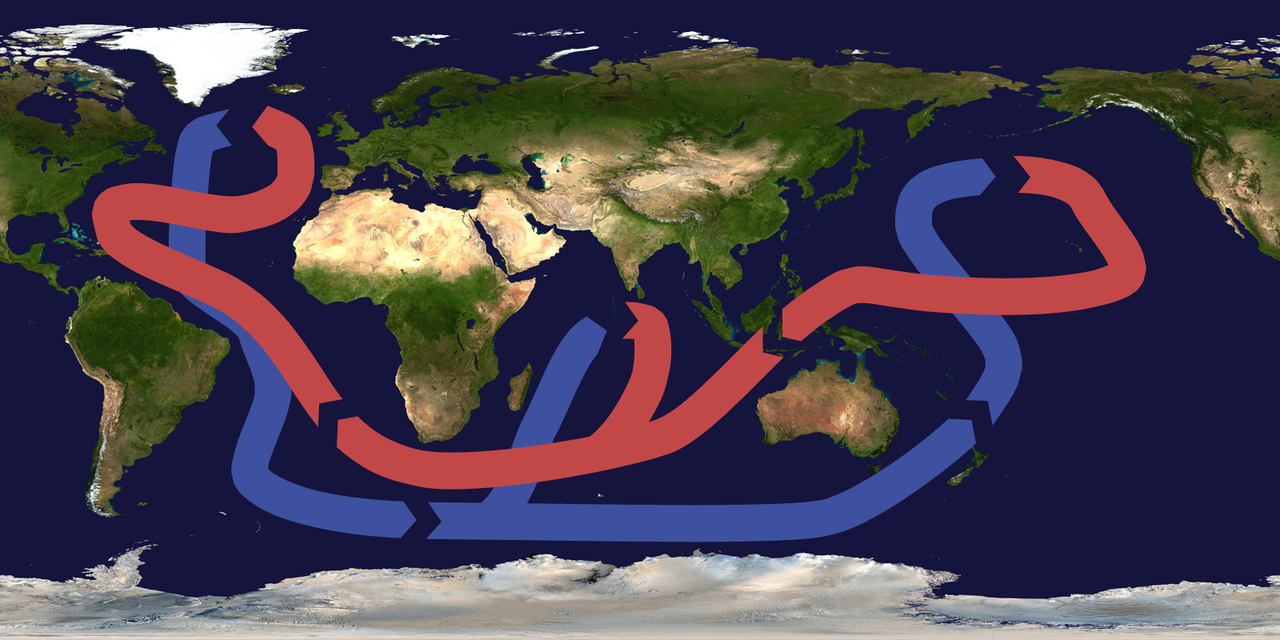
\includegraphics[width=\hsize]{chapters/4/1280px-Thermohaline_circulation.png}
\caption{
Das globale Förderband der thermohalinen Zirkulation.
\label{skript:thc:foerderband}}
\end{figure}%
Der Salzgehalt des Meerwassers ist nicht konstant,
hat aber ähnlich grossen Einfluss auf die Dichte wie die Temperatur.
Dies führt zu einer grossräumigen Zirkulationsströmung in den Weltmeeren,
genannt die thermohaline Zirkulation,
und damit zu einem weiteren bedeutenden Energietransportmechanismus.
Abbildung~\ref{skript:thc:foerderband} zeigt den Umfang der Zirkulation,
auch genannt das globale Förderband (conveyor belt).
Auf einer Zeitskala von Jahrzehnten bis Jahrhunderten wird Meerwasser 
und damit auch Wärmeenergie über Distanzen umgewälzt, welche mehrfach die
Erde umspannen.

Die Organismen, die in den oberen Wasserschichten absterben, sinken langsam
auf den Meeresgrund.
Ohne eine umfassende Umwälzung der Weltmeere würden die oberen Wasserschichten
mit der Zeit an Nährstoffen verarmen.
Die thermohaline Zirkulation stellt also auch die Versorgung der
Weltmeere mit Nährstoffen sicher.

Der Golfstrom ist ein kleiner Ausschnitt des globalen Förderbandes.
Die gut bekannte Bedeutung des Golfstroms für das europäische Klima 
deutet an, wie wichtig die thermohaline Zirkulation für das globale
Klima ist.
Es ist daher unerlässlich zu verstehen, was die Zirkulation antreibt und
wie sich der Klimawandel darauf auswirken könnte.

In diesem Kapitel soll die thermohaline Zirkulation modelliert werden.
Besonderes Augenmerk liegt dabei auf der Tatsache, dass dieses System
kippen kann.
Bei einer genügend grossen Änderung der Klimaparameter kann die Zirkulation
sich auf irreversible Art ändern.
Ein solches Ereignis hätte katastrophale Auswirkungen für das Klima.

%
% salinitaet.tex -- Salinität
%
% (c) 2018 Prof Dr Andreas Müller
%
\section{Salinität und Dichte}
\rhead{Salinität}
Der Salzgehalt des Meerwassers ist nicht konstant.
Er steigt an, wenn Wasser verdampf oder sich Eis bildet.
Er sinkt, wenn das Salz durch Niederschläge verdünnt wird.
Mit der Veränderung des Salzgehaltes geht auch eine Änderung
der Dichte einher.


%
% schichtung.tex -- Tiefenaufbau des Meeres
%
% (c) 2018 Prof Dr Andreas Müller, Hochschule Rapperswil
%
\section{Aufbau der Meere\label{section:thc:schichtung}}
\rhead{Aufbau der Meere}
\begin{figure}
\centering
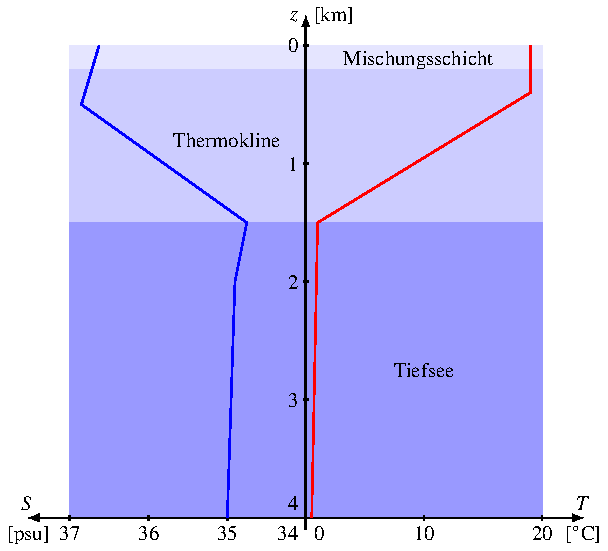
\includegraphics{chapters/4/schichten.pdf}
\caption{Tiefenaufbau des Meeres mit schematischem
Temperatur- und Salinitätsprofil.
Die Richtung der Achsen ist so gewählt, dass ``rechts'' gleichbedeutend
ist mit höher Dichte.
\label{skript:thc:schichtung}}
\end{figure}
Die Weltmeere umfassen etwa 1.4 Milliarden $\text{km}^3$ Wasser.
Wegen der hohen Wärmekapazität von $4.182\,\text{kJ}/\text{kg}\cdot\text{K}$
ist dies ein gigantisches Wärmereservoir mit entsprechend grosser
Bedeutung für das Klima.
Für das Verständnis des Klimassystems der Erde ist also die Kenntnis
des Aufbaus der Meere sowie des Energietransports in den Meeren unabdingbar.

Eine Reihe von Mechanismen beeinflussen Temperatur und Salinität.
An der Oberfläche wärmt sich das Wasser durch Einstrahlung
oder Zufluss warmen Wassers auf.
Wärmeaustausch mit der Atmosphäre gleicht die Temperatur von
Meer und Atmosphäre an, Verdunstung benötigt Energie und kühlt das Meer ab.
Der Zufluss von Süsswasser reduziert den Salzgehalt, die Verdungstung erhöht
die Salzkonzentration.
Durch Wind angeregte Turbulenz sorgt für gute Durchmischung dieser 
sogenannten {\em Mischungsschicht},
\index{Mischungsschicht}%
in ihr sind Temperatur und Salinität daher ungefähr konstant.
Sie reicht bis in eine Tiefe von wenigen hundert Metern.

In der Tiefe stehen bis auf einzelne wenige Stellen keine Quellen oder
Senken von Wärme oder Salz zur Verfügung.
Dort fehlt damit auch der Antrieb für Umwälzbewegungen, es bleibt
nur die Diffusion und die Schwerkraft.
Man kann daher davon ausgehen, dass in grosser Tiefe kaltes Wasser 
liegt mit weitgehend konstanter Temperatur und konstantem Salzgehalt.
Dies ist die {\em Tiefsee}.
\index{Tiefsee}%

Zwischen der Mischungsschicht und dem Tiefenwasser findet ein Ausgleich
von Temperatur und Salzgehalt statt.
Da dieser Ausgleich umso schneller erfolgt, je grösser der Unterschied
von Temperatur und Salinität erfolgt, ist ein Fliessgleichgewicht nur
möglich, wenn Temperatur und und Salinität in dieser Zone linear
von der Tiefe abhängen.
Diesen Bereich nennt man die {\em Thermokline}.
\index{Thermokline}%
Fehlt die Thermokline, hat das Oberflächenwasser die gleichen Eigenschaften
wie das Tiefenwasser, insbesondere gibt es keine Unterschiede, die eine
Umwälzung im Meer herbeiführen würden.
Je grösser tie Thermoklinentiefe, desto grösser auch der Unterschied
zwischen Obeflächenwasser und Tiefenwasser und desto mehr Energie für
den Antrieb der Zirkulation ist im Meer gespeichert.


%
% box.tex
%
% (c) 2018 Prof Dr Andreas Müller, Hochschule Rapperswil
%
\section{Ein Modell für die thermohaline Zirkulation}
\rhead{Ein Modell für die thermohaline Zirkulation}
Jedes numerische Modelle der Zirkulation basiert auf einer Diskretisation
des Gebietes.
Der Ozean wird also in kleine Teilgebiete aufgeteilt.
Gesucht sind Temperatur und Salinität in jedem Teilgebiet.
Dann werden Gleichungen aufgestellt, die den Austausch von Salz und
Wärme zwischen den Teilgebieten beschreiben.
Die Lösung dieser Gleichungen wird uns das Ausmass der Zirkulation zeigen
und erlauben abzuschätzen, wie sich die Zirkulation ändert, wenn sich
die äusseren Bedingungen verschieben.

\subsection{Ein einfaches Box-Modell}
Um einen ersten Eindruck von der Dynamik der thermohalinen Zirkulation
zu erhalten, verwenden wir ein Modell mit genau zwei Teilgebieten.
Wir modellieren den Atlantik nördlich des Äquators als zwei Gebiete.
Gebiet 1 ist das Polargebiet mit typischerweise tieferen Temperaturen,
Gebiet 2 ist das Gebiet in der Nähe des Äquators.
In jedem dieser Gebiet modellieren wir nur das Wasser, welches tatsächlich
von der Zirkulation umgewälzt wird.
Wir nehmen an, dass es sich durch die zwei Parameter Temperatur und
Salinität beschreiben lässt.
Wir bezeichnen die Variablen im Gebiet $i$ mit $T_i$ und $S_i$.

Das Wasser, welches an der Zirkulation teilnimmt, ist umgeben von einem
viel grösseren Wasserreservoir, welches mit dem strömenden Wasser 
im Wärme- und Salzaustausch steht.
Wir bezeichnen die konstanten Parameter dieser Reservoirs mit
$T_i^*$ und $S_i^*$.
In Abbildung~\ref{skript:boxmodell-bild} sind die beiden Gebiete
grau dargestellt, das in Zirkulation befindliche Wasser hellblau.
\begin{figure}
\centering
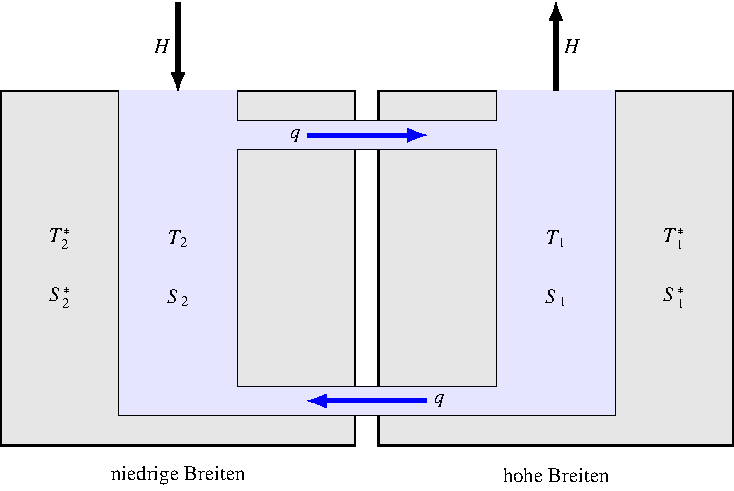
\includegraphics{chapters/4/boxmodell.pdf}
\caption{Einfaches Modell der thermohalinen Zirkulation
\label{skript:boxmodell-bild}}
\end{figure}

Die Zirkulation ist charakterisiert durch den Massefluss $q$ der
Tiefenströmung.
Da kein Wasser verloren gehen kann, muss in Oberflächennähe der gleiche
Fluss herrschen.
Da auch kein Salz verloren gehen kann, müssen sich auch die Salzflüsse
zwischen den beiden Gebieten ausgleichen.
Die Salinität wird zum Beispiel durch die Verdunstung erhöht, während
Niederschlag sie erniedrigt.
Süsswasserflüsse von Kontinenten reduzieren ebenfalls die Salinität.
Dies bedeutet, dass zusätzlich zum Massestrom $q$ ein virtueller 
Salzstrom zwischen den beiden Gebieten herrscht, den wir mit $H$ bezeichnen.

\subsection{Modell-Gleichungen\label{skript:thc:modell-gleichungen}}
Wir müssen jetzt Differentialgleichungen aufstellen, welche die
zeitliche Entwicklung von Temperatur $T_i(t)$ und Salinität $S_i(t)$
beschreiben kann.
Die Temperaturentwicklung wird bestimmt einerseits durch den Energietransport
durch den Fluss $q$ und andererseits durch den Wärmeaustausch mit dem
umgebenden Wasser.
Der Fluss $q$ hat zur Folge, dass sich die Temperaturen $T_1$ und $T_2$
angleichen.
Die beiden Flüsse oben und unten in Abbildung~\ref{skript:boxmodell-bild}
transportieren die gleiche Menge Wasser pro Zeiteinheit.
Es wird also gleichviel Wasser mit Temperatur $T_1$ ins Gebiet $2$ 
transportiert wie Wasser mit Temperatur $T_2$ ins Gebiet $1$.
Das Vorzeichen von $q$ spielt dabei keine Rolle, denn ändert das
Vorzeichen von $q$, fliesst das Wasser mit Temperatur $T_1$ einfach
durch den anderen Kanal.
Die Temperaturänderung von $T_1$ ist also proportional zu $|q|(T_2-T_1)$,
dies legt auch die Masseinheit von $q$ fest.

Der Wärmeaustausch mit dem umgebenden Wasser ist proportional zur
Temperaturdifferenz, wir bezeichnen den Proportionalitätsfaktor mit $c$.
Zusammen mit dem Wärmeaustausch durch die Strömung erhalten wir
die Differentialgleichungen
\begin{equation}
\begin{aligned}
\frac{dT_1}{dt}
&=
c(T_1^*-T_1)
+
|q|(T_2-T_1)
\\
\frac{dT_2}{dt}
&=
c(T_2^*-T_2)
+
|q|(T_1-T_2)
\end{aligned}
\label{skript:thc:temperaturgleichung}
\end{equation}
als Modell für die Temperaturentwicklung.

Analoge Überlegungen müssen wir jetzt auch noch für die Salinität anstellen.
Der Ausgleich der Salinität $S_i$ mit der Salinität $S_i^*$ des
umgebenden Meersbeckens ist proportional zur Differenz, der
Proportionalitätsfaktor, den wir mit $d$ bezeichnen, ist bestimmt durch
die Diffusionsgeschwindigkeit und die turbulente Durchmischung des
zirkulierenden Wassers mit der Umgebung.
Dazu kommt noch der virtuelle Salzfluss $H$:
\begin{equation}
\begin{aligned}
\frac{dS_1}{dt}
&=
\phantom{-}
H
+
d(S_1^*-S_1)
+
|q|(S_2-S_1)
\\
\frac{dS_2}{dt}
&=
-H
+
d(S_2^*-S_2)
+
|q|(S_1-S_2).
\end{aligned}
\label{skript:thc:salinitaetsgleichung}
\end{equation}
Man beachte, dass die Temperaturgleichungen~\eqref{skript:thc:temperaturgleichung}
und die Salinitätsgleichungen~\eqref{skript:thc:salinitaetsgleichung} 
gekoppelt sind, da der Fluss $q$ angetrieben wird vom Dichteunterschied,
der wiederum von Temperatur und Salinität abhängt.

\subsection{Antrieb der Zirkulation}
Die Zirkulation wird vom Dichteunterschied angetrieben.
Es gibt also einen Proportionalitätsfaktor $k$ derart, dass
\[
q = k\frac{\varrho_1 - \varrho_2}{\varrho_0}.
\]
Setzt man die Formel~\eqref{skript:salinity-linear} ein, findet man
\[
q
=
k(-\alpha(T_1-T_2) + \beta(S_1-S_2))
=
k(\alpha(T_2-T_1) + \beta(S_1-S_2))
=
k(\alpha(T_2-T_1) - \beta(S_2-S_1)).
\]
Schreiben wir $\Delta T = T_2-T_1$ und $\Delta S=S_2-S_1$,
dann ist der Fluss nur von den Differenzen abhängig:
\begin{equation}
q=k(\alpha\Delta T-\beta\Delta S).
\label{skript:thc:fluss-delta}
\end{equation}

\subsection{Anomalie-Gleichungen}
Die absoluten Werte von $T_i$ und $S_i$ sind nicht wirklich wichtig,
viel wichtiger sind die Unterschiede $\Delta T_i$ und $\Delta S_i$.
Verschwinden die Differenzen, kommt die Zirkulation zum erliegen,
und dies sind die Phänomene, die wir mit den Gleichungen prognostizieren
können möchten.
Wir streben daher an, die Gleichungen
\eqref{skript:thc:temperaturgleichung}
und
\eqref{skript:thc:salinitaetsgleichung}
in eine Form zu bringen, die nur von Differenzen und Anomalien
abhängt.

Wir schreiben
\[
T_0
=
\frac12(T_1+T_2)
\qquad\text{und}\qquad
S_0
=
\frac12(S_1+S_2)
\]
für die Mittelwerte von Temperatur und Salinität.
Indem wir den Mittelwert der Temperaturgleichungen
\eqref{skript:thc:temperaturgleichung}
bzw.~der Salinitätsgleichung \eqref{skript:thc:salinitaetsgleichung} bilden,
bekommen wir die Gleichungen
\begin{equation}
\begin{aligned}
\frac{dT_0}{dt}
&=
c(T_0^*-T_0)
\\
\frac{dS_0}{dt}
&=
d(S_0^*-S_0),
\end{aligned}
\label{skript:thc:mittelgleichung}
\end{equation}
wobei $T_0^* = \frac12(T_1^*+T_2^*)$ und $S_0^* = \frac12(S_1^*+S_2^*)$.
Die Differentialgleichungen~\eqref{skript:thc:mittelgleichung} 
besagen, dass die mittlere Temperatur des zirkulierenden Wassers
gegen die mittlere Temperatur des umliegenden Meeresbeckens strebt.
Die Faktoren $c$ und $d$ beschreiben, wie schnell der Temperaturausgleich
stattfindet, wie in Abschnitt~\ref{section:zeitkonstanten} ausgeführt wird.

Da die Mitteltemperatur langfristig gegen die Mitteltemperatur der
umliegenden Meeresbecken strebt, liegt es nahe, Temperatur und
Salinität auf diese Mitteltemperatur zu beziehen.
Wir ersetzen also
\begin{equation}
\begin{aligned}
\bar T_1&=T_1-T_0^*,
&
\bar T_2&=T_2-T_0^*
&&\Rightarrow&
\bar T_0&=T_0-T_0^*
\\
\bar S_1&=S_1-S_0^*,
&
\bar S_2&=S_2-S_0^*
&&\Rightarrow&
\bar S_0&=S_0-S_0^*
\end{aligned}
\end{equation}
Die Differentialgleichungen~\eqref{skript:thc:mittelgleichung}
für die Mittelwerte wird damit zu
\begin{align*}
\frac{d\bar T_0}{dt} &= -c \bar T_0\\
\frac{d\bar S_0}{dt} &= -d \bar S_0.
\end{align*}
Die Differentialgleichungen für
$T_i=\bar T_i + T_0^*$
und
$S_i=\bar S_i + S_0^*$
sind
\begin{align*}
\frac{dT_i}{dt}
&=
\frac{d\bar T_i}{dt}
=
c(T_i^*-T_i)
+ |q|\Delta \bar T
=
c(T_i^*- \bar T_i - T_0^*)
+ |q|\Delta \bar T
\\
\frac{dS_i}{dt}
&=
\frac{d\bar S_i}{dt}
=
\pm H
+
d(S_i^*-S_i)
+ |q|\Delta \bar S
=
\pm H
+
d(S_i^*- \bar S_i - S_0^*)
+ |q|\Delta \bar S
\end{align*}
Die Differenzen $T_i^*-T_0^*$ und $S_i^*-S_0^*$ können wir vereinfacht
als
\begin{align*}
T_1^*-T_0^* 
&=
T_1^* - \frac12(T_2^*-T_1^*)
=
-\frac12(T_2^*-T_1^*)
=
-T^*
\\
T_2^*-T_0^*
&=
T_2^*-\frac12(T_2^*-T_1^*)
=
\frac12(T_2^*-T_1^*)
=
T^*
\end{align*}
schreiben und analog für $S^*=\frac12(S_2^*-S_1^*)$.
Damit werden die Differentialgleichungen zu
\begin{equation}
\begin{aligned}
\frac{d\bar T_1}{dt}
&=
c(-T^*-\bar T_1) + |q| (\bar T_2-\bar T_1)
\\
\frac{d\bar T_2}{dt}
&=
c(T^*-\bar T_2) + |q| (\bar T_1-\bar T_2)
\\
\frac{d\bar S_1}{dt}
&=
-H
+
d(-S^*-\bar S_1) + |q|(\bar S_2 - \bar S_1)
\\
\frac{d\bar S_2}{dt}
&=
\phantom{-}H
+
d(S^*-\bar S_2) + |q|(\bar S_1 - \bar S_2)
\end{aligned}
\label{skript:thc:anomaliegleichungen}
\end{equation}
Man beachte, dass die $T^*$ und $S^*$ konstant sind.

In den Gleichungen~\eqref{skript:thc:anomaliegleichungen} hängt
$q$ von den Temperatur- und Salinitätsdifferenzen ab.
Wegen $\Delta\bar T=\Delta T$ und $\Delta\bar S=\Delta S$ ist nach
\eqref{skript:thc:fluss-delta}
\begin{equation}
q = k(\alpha\Delta\bar T-\beta \Delta\bar S).
\label{skript:thc:fluss-delta-anomalie}
\end{equation}

\subsection{Differenzgleichungen}
Wir können die Anomaliegleichungen \eqref{skript:thc:anomaliegleichungen}
noch etwas weiter umformen und die einzelnen Ano\-malien vollständig durch
die Differenzen ersetzen.
Die Differenzen und Summen der Gleichungen sind
\begin{equation}
\begin{aligned}
\frac{d\Delta\bar T}{dt}
&=
c(2T^*-\Delta\bar T)-2|q|\Delta\bar T
&&\qquad&
\frac{d\bar T_0}{dt}
&=
-c\bar T_0
\\
\frac{d\Delta\bar S}{dt}
&=
2H+d(2S^*-\Delta\bar S) - 2|q|\Delta\bar S
&&\qquad&
\frac{d\bar S_0}{dt}
&=
-d\bar S_0.
\end{aligned}
\label{skript:thc:differenzgleichungen}
\end{equation}
Die Gleichungen rechts drücken aus, dass die mittleren Anomalien
exponentiell gegen $0$ gehen.
Die linken Gleichungen beschreiben die Zeitentwicklung der Differenz
der Anomalien.
Man beachte, dass $q$ ebenfalls von den Anomalie-Differenzen abhängt.

\subsection{Zeitkonstanten\label{section:zeitkonstanten}}
\label{skript:thc:zeitkonstanten}
Der Koeffizienten $c$ beschreibt, wie schnell der Temperaturausgleich
durch Wärmeleitung oder turbulente Durchmischung erfolgt.
Der Koeffizient $d$ beschreibt, wie schnell der Salinitätsausgleich
durch Durchmischung und Diffusion stattfinden kann.
Je grösser diese Koeffizienten, desto schneller erfolgt der Prozess.
In den rechten Gleichungen von \eqref{skript:thc:differenzgleichungen}
ist dies ganz offensichtlich.
Vernachlässigen wir für den Moment den Einfluss der Zirkulation,
was wir durch $k=0$ im Ausdruck für $q$ beschreiben können, dann
sehen wir, dass die Differenzgleichungen beide von der Form
einer linearen inhomogenen Differentialgleichung
\[
\frac{d\Delta X}{dt}
=
X^* -cX
\]
sind, wobei $X^*$ eine Konstante ist.
Die Lösung der Gleichung ist
\[
X(t) = \frac{X^*}{c} + C_0 e^{-ct}
\]
mit einer Konstanten $C_0$, die aus den Anfangsbedingungen zu
bestimmen ist.
Die Terme $T^*$, $S^*$ und $H$ verschieben also nur die Lösung,
die Differenzen $\Delta\bar T$ und $\Delta\bar S$ streben exponentiell
wie $e^{-ct}$ bzw.~$e^{-dt}$ gegen diese Gleichgewichtswerte.

Die Grössen $1/c$ und $1/d$ haben die Dimension einer Zeit, wir nennen
sie die {\em Zeitkonstanten} des Prozesses, den $c$ bzw.~$d$ beschreiben.
\index{Zeitkonstante}
Ist zum Beispiel die Zeitkonstante $1/c$ der Temperatur sehr viel kleiner
als die Zeitkonstanten $1/d$ der Salinität, dann bedeutet dies, dass
sich die Temperaturdifferenzen sehr viel schneller ausgleichen als die
Salinitätsdifferenzen.
Für die langfristige Entwicklung der Zirkulation ist in diesem Fall
die Salinitätsentwicklung ausschlaggebend, die Temperaturfunktionen
können durch Konstanten ersetzt werden.





%
% dimensionslos.tex
%
% (c) 2018 Prof Dr Andreas Müller, Hochschule Rapperswil
%
\section{Dynamik der thermohalinen Zirkulation}
\rhead{Dynamik der thermohalinen Zirkulation}
In diesem Abschnitt wollen wir die
Bewegungsgleichung~\eqref{skript:thc:differenzgleichungen}
etwas vereinfachen mit dem Ziel, einzelne Szenarien durchspielen
zu können.
Eine vertiefte Diskussion solcher Modelle ist in
Kapitel~\ref{chapter:thermohalin} zu finden.

\subsection{Elimination von Prozessen mit kurzer Zeitkonstante}
Die Diskussion in Abschnitt~\ref{skript:thc:zeitkonstanten}
ist es zulässig, Variablen mit sehr kleiner Zeitkonstanten
durch Konstanten zu ersetzen.
Tatsächlich erfolgt der Temperaturausgleich im Wasser sehr viel
schneller als der Salinitätsausgleich.
Wir können daher davon ausgehen, dass die Temperaturgleichungen
die Temperaturanomalien sehr schnell gegen eine Gleichgewichtstemperatur
streben lassen und dass wir für die Lösung der Salinitätsgleichungen
mit dieser konstanten Temperatur arbeiten können.

Wir gehen also davon aus, dass $\Delta\bar T=2T^*$ konstant ist und
reduzieren damit das Gleichungssystem
\eqref{skript:thc:differenzgleichungen}
auf die eine Gleichung
\begin{equation}
\frac{d}{dt}\Delta\bar S
=
2H + d(2S^* -\Delta\bar S) - 2|q|\Delta\bar S
\qquad\text{mit}\qquad
q=k(2\alpha T^* -\beta \Delta\bar S).
\label{skript:thc:salinitaetallein}
\end{equation}
Diese Gleichungen beschreiben also die Salinitätsentwicklung unter
der Annahme, dass der Temperaturausgleich sehr schnell erfolgt.
Dieser Ausgleich kann nicht primär durch Durchmischung erfolgen,
denn dieser Mechanimus würde auch die Salinität mit gleicher
vergleichbarer Geschwindigkeit ausgleichen.
Dies bedeutet, dass der dominante Term in der Temperaturgleichung
der Term mit $c$ ist, nicht der Term mit $q$.

Die Gleichung \eqref{skript:thc:salinitaetallein} kann noch nicht auf
einfache Weise gelöst werden.
Wir vereinfachen wir sie daher weiter indem wir ausnutzen, dass 
der Salinitätsausgleich so viel langsamer ist als der Temperaturausgleich,
dass der Term mit $d$ im Vergleich zum Term mit $q$ vernachlässigbar ist.
Wir setzen also $d=0$ und
erhalten damit 
\begin{equation}
\frac{d}{dt}\Delta\bar S
=
2H - 2|q|\Delta\bar S
\qquad\text{mit}\qquad
q=k(2\alpha T^* -\beta \Delta\bar S)
\label{skript:thc:qgleichung}
\end{equation}
als vereinfachte Differentialgleichung zur Modellierung der 
thermohalinen Zirkulation.
Dies ist eine nichtlineare Differentialgleichung erster Ordnung,
die nicht in geschlossener Form gelöst werden kann.

\subsection{Eine dimensionslose Beschreibung}
Die Gleichung \eqref{skript:thc:qgleichung} ist wegen der vielen
Konstanten unübersichtlich.
Ausgeschrieben lautet sie
\begin{equation}
\frac{d}{dt}\Delta\bar S
=
2H
-2k\,|\alpha\Delta\bar T- \beta \Delta\bar S|\,\Delta\bar S
\label{skript:thc:smitdim}
\end{equation}
Die meisten der Konstanten können wir aber los werden, indem wir 
die unabhängigen Variablen und die Zeit neu skalieren.
Dies ist gleichbedeutend mit einem Wechsel der Masseinheiten.
Wir verwenden:
\begin{equation}
x=\frac{\beta\Delta\bar S}{\alpha\Delta\bar T},
\qquad
\tau = 2\alpha k\,|\Delta\bar T|\, t
\qquad\text{und}\qquad
\lambda = \frac{\beta H}{\alpha^2 k\Delta\bar T|\Delta\bar T|}.
\label{skript:thc:masseinheiten}
\end{equation}
Die Ableitung nach $t$ kann durch die Ableitung nach $\tau$ ausgedrücket
werden vermöge der Ersetzung
\[
\frac{d}{d\tau}
=
\frac{1}{2\alpha k|\Delta\bar T|}
\frac{d}{dt}
\qquad\Rightarrow\qquad
\frac{d}{dt}
=
2\alpha k|\Delta\bar T|\frac{d}{d\tau}.
\]
Setzen wir dies in die Gleichung~\eqref{skript:thc:masseinheiten}
ein, erhalten wir
\begin{equation}
2\alpha k|\Delta\bar T|
\frac{d}{d\tau} \Delta\bar S
=
2H-2k|\alpha\Delta\bar T-\beta\Delta\bar S|\,\Delta\bar S.
\end{equation}
Wir erweitern mit $\beta/\alpha\Delta\bar T$, damit wird die
Differentialgleichung zu
\begin{align}
2\alpha k|\Delta\bar T|
\frac{d}{d\tau}\frac{\beta\Delta\bar S}{\alpha\Delta\bar T}
&=
\frac{2\beta H}{\alpha\Delta\bar T} - 2k|\alpha\Delta\bar T-\beta\Delta\bar S|\,
\frac{\beta\Delta\bar S}{\alpha\Delta\bar T}
\notag
\\
\alpha k|\Delta\bar T|
\frac{d}{d\tau}x
&=
\frac{\beta H}{\alpha\Delta\bar T}
-k|\alpha\Delta\bar T-\beta\Delta\bar S|\, x
\notag
\\
k
\frac{d}{d\tau}x
&=
\frac{\beta H}{\alpha^2\Delta\bar T\,|\Delta\bar T|}
-k\biggl|1-\frac{\beta\Delta\bar S}{\alpha\Delta\bar T}\biggr|\,x
\notag
\\
\frac{d}{d\tau}x
&=
\frac{\beta H}{k\alpha^2\Delta\bar T\,|\Delta\bar T|}
-\biggl|1-\frac{\beta\Delta\bar S}{\alpha\Delta\bar T}\biggr|\,x
\notag
\\
\frac{dx}{d\tau}
&=
\lambda - |1-x|x.
\label{skript:thc:dimensionslos}
\end{align}
Damit haben wir die ursprüngliche Gleichung
\eqref{skript:thc:smitdim}
in eine dimensionslose Gleichung mit dem einen Parameter $\lambda$
umgewandelt.
%Das Verhalten der Lösung hängt vom Parameter $\lambda$ ab.

\subsection{Gleichgewicht}
Um das Verhalten der Lösungen von 
\eqref{skript:thc:dimensionslos}
besser zu verstehen, suchen wir zunächst nach Gleichgewichtslösungen.
Diese hängen nicht von der Zeit ab, es gilt also
\begin{equation}
\frac{dx}{d\tau}=0
\qquad\Rightarrow\qquad
\lambda-|1-x|x=0
\qquad\Rightarrow\qquad
|1-x|x
=
\lambda.
\label{skript:thc:lambdagl}
\end{equation}
\begin{figure}
\centering
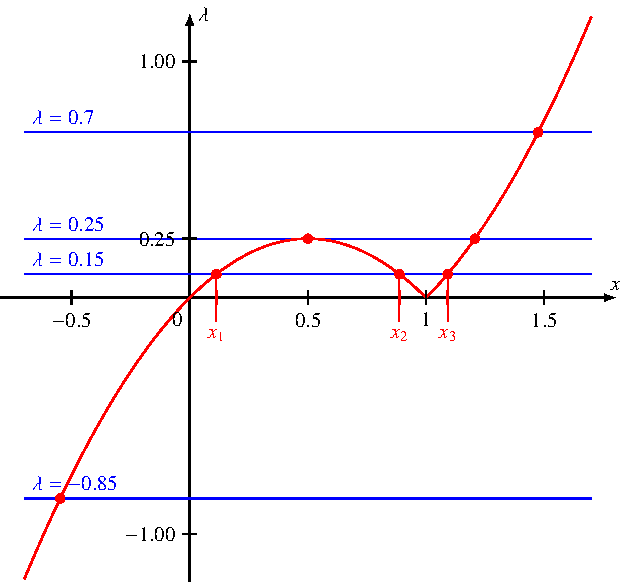
\includegraphics{chapters/4/rhs.pdf}
\caption{Graph der Funktion $|1-x|\,x$ und
Gleichgewichtslösungen der dimensionslosen Differentialgleichung
\eqref{skript:thc:dimensionslos}
\label{skript:thc:1-xxgraph}}
\end{figure}%
In Abbildung~\ref{skript:thc:1-xxgraph} ist der Graph der Funktion 
$|1-x|\,x$ dargestellt.
Je nach dem Wert von $\lambda$ hat die dimensionslose Differentialgleichung
\eqref{skript:thc:dimensionslos} bis zu drei Gleichgewichtslösungen.

Für Werte von $\lambda$ zwischen $0$ und $0.25$ gibt es drei verschiedene
Werte $x$, die die Gleichung \eqref{skript:thc:lambdagl} erfüllen
(Abbildung~\ref{skript:thc:drei}).
Für $x\le 1$  ist $1-x\ge 0$ und damit muss $x$ die 
Gleichung $(1-x)x=\lambda$ erfüllen, für $x\ge 1$ ist es die Gleichung
$(x-1)x=\lambda$.
Diese beiden Gleichungen haben die folgenden Lösungen
\begin{align*}
&\text{Fall $x \le 1$:}
&
(1-x)x&=\lambda
&
&\text{Fall $x\ge 1$:}
&
(x-1)x&=\lambda
\\
&&
x^2-x+\lambda&=0
&&&
x^2-x-\lambda&=0
\\
&&
x&=\frac12\pm\sqrt{\frac14-\lambda}
&&&
x&=\frac12+\sqrt{\frac14+\lambda}.
\end{align*}
Die rechte Gleichung hat für alle Werte $\lambda > 0$ zwar auch noch
eine Lösung $<1$, diese ist aber ausgeschlossen, daher nur das
positive Zeichen vor der Wurzel in diesem Fall.
Für $\lambda > 0.25$ hat die linke Gleichung keine Lösung.
Für $\lambda < 0$ ist die Lösung mit dem positiven Zeichen der linken
Gleichung ausgeschlossen.

\begin{figure}
\centering
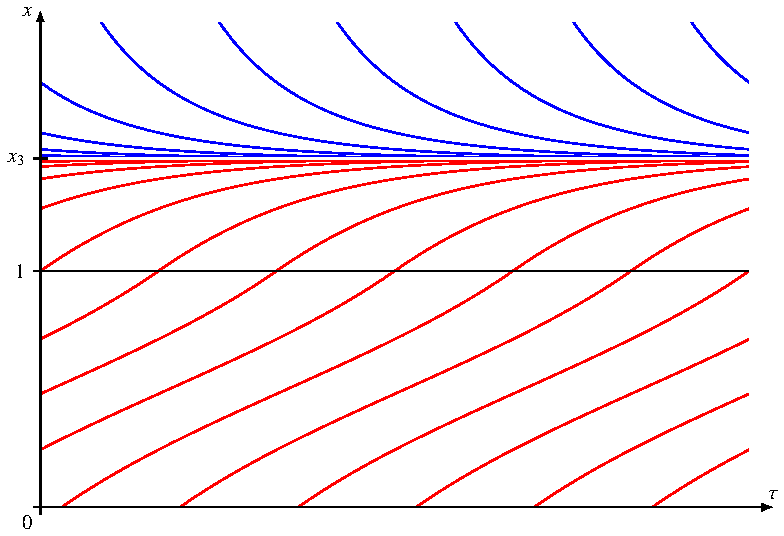
\includegraphics{chapters/4/ein.pdf}
\caption{Lösungen im Fall $\lambda > \frac14$: der einzige
Gleichgewichtspunkt $x_3$ ist stabil.
\label{skript:thc:ein}}
\end{figure}%
Wir berechnen die Lösung der Differentialgleichung für einen gegebenen
Wert von $\lambda$ (Abbildung~\ref{skript:thc:ein}).
Für $\lambda >\frac14$ gibt es nur einen Gleichgewichtspunkt, wir 
nennen ihn $x_3$.
Falls $x(\tau)<x_3$, dann ist
\[
\frac{dx}{d\tau}
=
\lambda - |1-x|x > 0,
\]
die Lösung $x(\tau)$ ist also monoton wachsend.
Für $x(\tau) > x_3$ ist hingegen
\[
\frac{dx}{d\tau}
=
\lambda - |1-x|x < 0,
\]
die Lösung ist also monoton fallend.
Lösungskurven, die bei $x$-Werten $>x_3$ beginnen nehmen monoton ab
und konvergieren gegen $x_3$, solche, die bei $x$-Werten $<x_3$ beginnen,
nehmen monoton zu und konvergieren von unten gegen $x_3$.
Die Gleichgewichtslösung $x(\tau)=x_3$ ist also eine stabile Lösung,
alle anderen Lösungen konvergieren gegen diese Lösung.

\begin{figure}
\centering
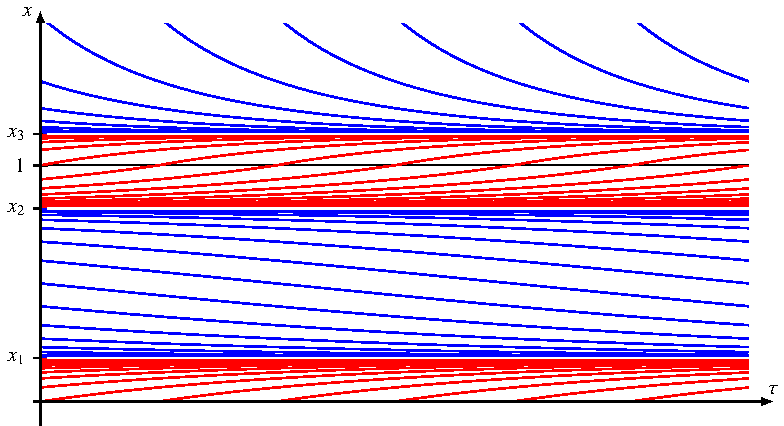
\includegraphics{chapters/4/drei.pdf}
\caption{Lösungen im Fall $0\le \lambda\le\frac14$: die beiden
Gleichgewichtspunkte $x_1$ und $x_3$ sind stabil, $x_2$ ist instabil.
\label{skript:thc:drei}}
\end{figure}%
Für $0<\lambda<\frac14$ seien
$x_1$, $x_2$ und $x_3$ die drei Gleichgewichtspunkte
(Abbildung~\ref{skript:thc:drei}).
Wir untersuchen wieder die Vorzeichen von $dx/d\tau$. 
Für $x$-Werten zwischen $x_1$ und $x_2$ und für $x$-Werte grösser
als $x_3$ ist die Ableitung positiv, die Lösungen konvergieren monoton
wachsend gegen die Gleichgewichtslösungen $x_1$ bzw.~$x_3$.
Lösungen, die bei $x<x_1$ oder $x_2<x<x_3$ beginnen, konvergieren
dagegen monoton wachsend gegen $x_1$ bzw.~$x_3$.
Die Gleichgewichtslösung $x_2$ ist daher nicht stabil,
die Gleichgewichtslösungen $x_1$ und $x_3$ sind dagegen stabil.

\subsection{Bifurkation}
In diesem Abschnitt studieren wir die Abhängigkeit der Gleichgewichtslösungen
in Abhängigkeit vom Parameter $\lambda$, wie dies in Abschnitt
\ref{section:bifurkation-eindim} vorbereitet wurde.

\begin{figure}
\centering
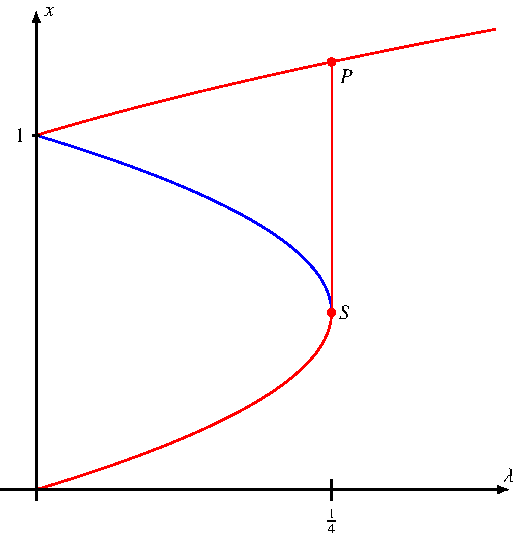
\includegraphics{chapters/4/bi.pdf}
\caption{Bifurkationsdiagramm für die Differentialgleichung
\eqref{skript:thc:lambdagl}
\label{skript:thc:bifurkation}}
\end{figure}
Für Parameterwerte $\lambda < \frac14$ gibt es drei mögliche
Gleichgewichtspunkte, für $\lambda>\frac14$ jedoch nur noch einen.
Wir möchten untersuchen, wie sich die Lösung verhält, wenn der
Parameter langsam verändert wird.
Dies ist in Abbildung~\ref{skript:thc:bifurkation} dargestellt.

Sei jetzt also zunächst $\lambda <\frac14$.
Wir betrachten eine Lösung, die in Nähe von
\[
x_1(\lambda)=\frac12-\sqrt{\frac14-\lambda}
\]
beginnt.
Vergrössern wir $\lambda$, verschiebt sich der Gleichgewichtspunkt
$x_1(\lambda)$ ebenfalls nach oben.
Da $x_1(\lambda)$ aber ein stabiler Gleichgewichtspunkt ist, wird die
Lösung gegen den neuen Gleichgewichtspunkt konvergieren.
Das gleiche passiert auch, wenn die Lösung in der Nähe von
\[
x_3(\lambda)=\frac12+\sqrt{\frac14+\lambda}
\]
beginnt.
Bei einer Vergrösserung folgt das System den roten Kurven in
Abbildung~\ref{skript:thc:bifurkation}.

Wenn jetzt aber der Parameter $\lambda$ die Schwelle $\frac14$
überschreitet, dann wird die Lösung zum einzigen verbleibenden
stabilen Gleichgewichtspunkt $x_3(\lambda)$ konvergieren.
Die Lösung springt also vom Punkt $S$ zum Punkt $P$ auf dem oberen roten Ast
in Abbildung~\ref{skript:thc:bifurkation}.

Wenn man den Parameter $\lambda$ wieder verkleinert, dann wird
eine Lösung in der Nähe von $x_3(\lambda)$ wieder gegen
$x_3(\lambda)$ konvergieren.
Es ist aber nicht mehr möglich, dass die Lösung gegen $x_1(\lambda)$
konvergiert, da nach Abbildung~\ref{skript:thc:drei} nur Lösungen,
die bei $x$-Werten $<x_2$ beginnen, gegen $x_1(\lambda)$ konvergieren
können.

Dieses einfache Modell der thermohalinen Zirkulation hat also die
überraschende Eigenschaft, dass das System beim Überschreiten des
kritischen Wertes $\lambda=\frac14$ in einen Zustand kippt, aus dem
es nicht mehr zurück kommen kann.
Wegen
\[
\lambda
=
\frac{\beta H}{\alpha^2k\Delta\bar T\,|\Delta\bar T|}
\]
kann dies passieren wenn entweder der Betrag des virtuellen Salzflusses 
$H$ ansteigt oder die Temperaturanomaliedifferenz $\Delta\bar T$
klein wird.
Eine Klimaerwärmung könnte zum Beispiel die Verdunstung im Gebiet $2$
erhöhen, den virtuellen Salzfluss erhöhen und damit das System
in den Zustand mit einer wesentlich grösseren Anomaliedifferenz
$\Delta\bar S$ kippen lassen.









		% 4
%
% zonen.tex -- Zonenmodelle für das Klima
%
% (c) 2018 Prof Dr Andreas Müller, Hochschule Rapperswil
%
\chapter{Zonenmodelle\label{chapter:zonenmodelle}}
\lhead{Kapitel \thechapter: Zonenmodelle}
Die Erdrotation ist schnell im Vergleich zu den für typische Klimamodelle
wesentlichen Zeitspannen.
Wesentliche Aspekte der Klimaentwicklung sollten sich daher immer
noch modellieren lassen, wenn man den Zustand des Klimasystems über
die Erdrotation mittelt.
In diesem Kapitel werden daher vereinfachte Modelle diskutiert,
die nur die geographischen Länge als geometrischen Parameter haben.

%
% strahlung.tex
%
% (c) 2018 Prof Dr Andreas Müller, Hochschule Rapperswil
%
\section{Strahlung\label{section:strahlung}}
\rhead{Strahlung}
Die von der Erde empfange Strahlung sowie die Albedo wurden bereits in
Abschnitt~\ref{skript:grundlagen:strahlung} untersucht.
Für die später in diesem Kapitel zu untersuchenden Modelle ist aber
erforderlich, die örtliche Verteilung der Strahlung auf der Erdoberfläche
genauer zu verstehen.
In diesem Abschnitt wird daher zuerst die Strahlungsleistung auf einer
Halbkugel und später auf einer Zone um einen Breitenkreis berechnet.
%
% halbkugel.tex -- Einstrahlung auf eine Halbkugel
%
% (c) 2018 Prof Dr Andreas Müller, Hochschule Rapperswil
%
\subsection{Einstrahlung auf einer Halbkugel\label{subsection:halbkugel}}
\begin{figure}
\centering
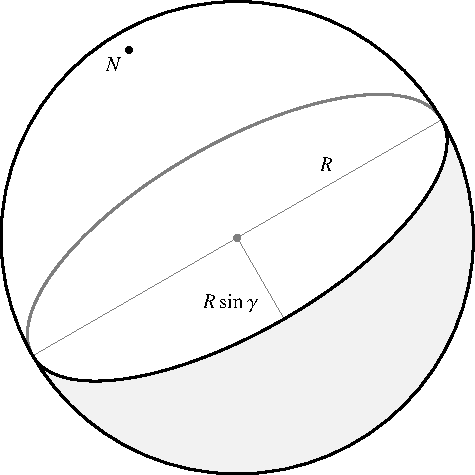
\includegraphics{chapters/5/halb.pdf}
\caption{Aufteilung der sonnenbeschienenen Seite der Erde durch den
Äquator.
\label{skript:halbkugel:teilung}}
\end{figure}%
Die einfachste Erweiterung des Modells von Budyko teilt die
Erde in zwei Halbkugeln auf, die Energie nur langsam austauschen
können.
Für die Energiebilanz brauchen wir daher die Strahlungsleistung
auf einer Halbkugel in Abhängigkeit von der Neigung $\gamma$ der
Erdachse.

Die gesamte auf auf die Erde eingestrahlte Leistung ist $\pi R^2S_0$.
Diese Leistung muss nun in Abhängigkeit von der Neigung $\gamma$
auf die beiden Halbkugeln verteilt werden.
Von der Erde aus gesehen teilt der Äquator die bestrahlte Erde wie
in Abbildung~\ref{skript:halbkugel:teilung} dargestellt.
Der Unterschied zwischen den beiden Halbkugeln ist der Flächeninhalt
der Ellipse, also
\[
F=\pi R^2\sin\gamma.
\]
Die Strahlungsleistung auf den beiden Halbkugeln in
Abbildung~\eqref{skript:halbkugel:teilung} ist daher
\begin{align}
E_N
&= 
\frac12(\pi R^2 S_0 +\pi R^2S_0\sin\gamma)
=
\pi R^2S_0 \frac{1+\sin\gamma}2 = Q\frac{1+\sin\gamma}2
&&\text{Nordhalbkugel,}
\\
E_S
&= 
\frac12(\pi R^2 S_0 -\pi R^2\sin\gamma)
=
\pi R^2S_0 \frac{1-\sin\gamma}2 = Q\frac{1-\sin\gamma}2
&&\text{Südhalbkugel.}
\end{align}
In Kapitel~\ref{chapter:neigung} wird diese Lösung verwendet, um zu
modellieren, wie die Veränderung der Neigung der Erdachse zu Eiszeiten
führen kann.





%
% einstrahlung.tex
%
% (c) 2018 Prof Dr Andreas Müller,Hochschule Rapperswil
%
\subsection{Einstrahlung auf einen Breitenkreis}
Wir berechnen die Einstrahlung auf einem gegebenen Breitengrad
$\vartheta$ in Abhängigkeit von der Neigung $\gamma$
der Erdachse.
Die einfallende Strahlungsleistung ist proportional zum Skalarprodukt
der Richtung der Einstrahlung mit der Normalen in einem Punkte
auf dem Breitenkreis zur Breite $\vartheta$.
Die Normale ist
\[
\vec n(\vartheta,\varphi)
=
\begin{pmatrix}
\sin\vartheta\cos\varphi\\
\sin\vartheta\sin\varphi\\
\cos\vartheta
\end{pmatrix}.
\]
Die Richtung der Einstrahlungsrichtung ist
\[
\vec e(\gamma)
=
\begin{pmatrix}
\cos\gamma\\
0\\
\sin\gamma
\end{pmatrix}.
\]
Das Skalarprodukt ist
\begin{equation}
\vec n(\vartheta,\varphi)\cdot\vec e(\gamma)
=
\sin\vartheta\cos\varphi\cos\gamma
+
\cos\vartheta\sin\gamma.
\label{skript:einstrahlung:skalarprodukt}
\end{equation}
Für die folgende Diskussion nehmen wir an, dass $\gamma >= 0$,
dass also der Nordpol permanent bestrahlt ist und der Südpol keine
Strahlung erhält.

Im Folgenden wollen wir die Energie berechnen, die in eine Zone
eingestrahlt wird.

\subsubsection{Sonnenauf- und -untergang}
Die Einstrahlung erfolgt natürlich nur zwischen Sonnenauf- und
-untergang.
Wir bezeichen die geographische Länge, bei der der Sonnenauf- oder
-untergang erfolgt, mit $\pm\varphi_0$.
Diese sind gekennzeichnet dadurch, dass $\vec n(\vartheta,\varphi_0)$ und
$\vec e(\gamma)$ senkrecht aufeinander stehen oder
\begin{equation*}
\begin{aligned}
&&
\vec n(\vartheta,\varphi_0)&\perp \vec e(\gamma)
\\
&\Rightarrow&
\vec n(\vartheta,\varphi_0)\cdot \vec e(\gamma)&=0
\\
&\Rightarrow&
\sin\vartheta\cos\varphi_0\cos\gamma
&=
-
\cos\vartheta\sin\gamma
\\
&\Rightarrow&
\cos\varphi_0
&=
-\frac{\tan\gamma}{\tan\vartheta}.
\end{aligned}
\end{equation*}
Wenn $\vartheta < \gamma$ (Punkt in der Nähe des Nordpols) oder
$\vartheta > \pi - \gamma$ (Punkt in der Nähe des Südpols),
dann hat die Gleichung keine Lösung,
die Sonne geht nie auf (Polarnacht) oder unter (Polartag).

\subsubsection{Mittlere Strahlungsleistung auf Breite $\vartheta$}
Um die Strahlungsleistung auf einer beliebigen geographischen
Breite zu berechnen, gehen wir in zwei Schritten vor.
Das Skalarprodukt~\eqref{skript:einstrahlung:skalarprodukt} 
gibt die Strahlungsleistung $\varepsilon(\vartheta,\varphi,\gamma)$
in einem Punkt auf der geographischen
Breite $\vartheta$ in Abhängigkeit von $\varphi$.
Im ersten Schritt mitteln wir dies über eine Umdrehung, dazu
ist das Skalarprodukt~\eqref{skript:einstrahlung:skalarprodukt} über eine
Umdrehung zu mitteln.
So erhalten wir die mittlere Strahlungsleistung $\varepsilon(\vartheta,\gamma)$
in einem Punkte auf geographischer Breite $\vartheta$.
Im zweiten Schritt müssen wir die die mittlere Strahlungsleistung mit
der Länge des Breitenkreises multiplizieren, um die Strahlungsleistung
auf dem Breitenkreis zur Breite $\vartheta$ zu erhalten.

\subsubsection{Polnähe}
In der Nähe des Südpols, also wenn $\vartheta > \pi - \gamma$,
ist die Einstrahlung $=0$.
In der Nähe des Nordpols, also wenn $\vartheta < \gamma$, ist die
Einstrahlungsdichte
\[
\varepsilon_{\text{in}}
=
\int_0^{2\pi}
\sin\vartheta\cos\varphi\cos\gamma
+
\cos\vartheta\sin\gamma
\,d\varphi
=
2\pi\cos\vartheta\sin\gamma.
\]
Für den Spezialfall $\vartheta=0$ fällt der erste Term weg und es
bleibt 
\begin{align*}
\varepsilon_{\text{in}}(0,\gamma)
&=
2\pi\sin\gamma.
\end{align*}

\subsubsection{Äquator}
Am Äquator ist $\vartheta=\frac{\pi}2$ und $\varphi_0=\frac{\pi}2$.
Man bekommt
\begin{align*}
\varepsilon_{\text{in}}\biggl(\frac{\pi}2,\gamma\biggr)
&=
\int_{-\varphi_0}^{\varphi_0}
\cos\varphi\cos\gamma\,d\varphi
=
\cos\gamma
\int_{-\frac{\pi}2}^{\frac{\pi}2}
\cos\varphi
\,d\varphi
=
2\cos\gamma
\end{align*}
für die Einstrahlung am Äquator.

\subsubsection{Der allgemeine Fall mit Sonnenauf- und -untergang}
\begin{figure}
\centering
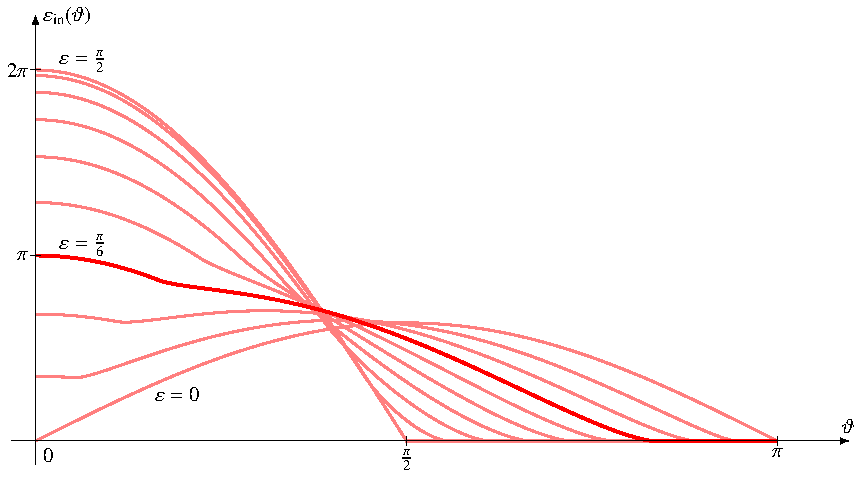
\includegraphics[width=\hsize]{chapters/5/ein.pdf}
\caption{Über eine Rotation gemittelte Einstrahlungsdichte
in Abhängigkeit von der geographischen Breite
gemäss Formel~\eqref{skript:einstrahlung:plottable} für verschiedene
Neigungen $\gamma$ der Achse. 
Dargestellt sind $\gamma$-Werte zwischen 0 und $90^\circ$ 
in $10^\circ$-Schritten. 
Die Neigung $\gamma=30^\circ=\frac{\pi}{6}$ ist hervorgehoben.
\label{skript:einstrahlung:ein}}
\end{figure}%
Der allgemeine Fall mit Sonnenauf- und -untergang
ist $\gamma < \vartheta < \pi-\gamma$.
Für die Einstrahlung finden wir dann
\begin{align}
\varepsilon_{\text{in}}(\vartheta,\gamma)
&=
\int_{-\varphi_0}^{\varphi_0}
\sin\vartheta\cos\varphi\cos\gamma
+
\cos\vartheta\sin\gamma\,d\varphi
\notag
\\
&=
\sin\vartheta\cos\gamma\biggl[\sin\varphi\biggr]_{-\varphi_0}^{\varphi_0}
+
2\varphi_0 \cos\vartheta\sin\gamma
\notag
\\
&=
2\sin\vartheta\cos\gamma\sin\varphi_0
+
2\varphi_0 \cos\vartheta\sin\gamma
\notag
\\
&=
2\sin\vartheta\cos\gamma
\sin
\arccos\biggl(-\frac{\tan\gamma}{\tan\vartheta}\biggr)
+
2\cos\vartheta\sin\gamma
\arccos\biggl(-\frac{\tan\gamma}{\tan\vartheta}\biggr).
\notag
\\
\intertext{Im ersten Term können wir $\sin\arccos x  = \sqrt{1-x^2}$
verwenden.
Den zweiten Term könnten wir so stehen lassen, aber für die graphische
Darstellung brauchen wir eine Darstellung das Arkuskosinus durch den
Arkustangens, da TikZ nur den Arkustangens anbietet.
Wir verwenden die Formel $\arccos x = 2\arctan\sqrt{(1-x)/(1+x)}$ und
erhalten}
&=
2\sin\vartheta\cos\gamma
\sqrt{1-\frac{\tan^2\gamma}{\tan^2\vartheta}}
+
4\cos\vartheta\sin\gamma
\arctan\sqrt{\frac{1+\frac{\tan\gamma}{\tan\vartheta}}{1-\frac{\tan\gamma}{\tan\vartheta}}}
\notag
\\
&=
\pm2\cos\vartheta\cos\gamma
\sqrt{\tan^2\vartheta-\tan^2\gamma}
+
4\cos\vartheta\sin\gamma
\arctan\sqrt{\frac{\tan\vartheta+\tan\gamma}{\tan\vartheta-\tan\gamma}}
\notag
\\
&=
2
\cos\vartheta
\biggl(
\cos\gamma
\sqrt{\frac{\tan^2\vartheta}{\tan^2\gamma}-1}
+
2
\sin\gamma
\arctan\sqrt{
\frac{\tan\vartheta+\tan\gamma}{\tan\vartheta-\tan\gamma}
}
\biggr).
\label{skript:einstrahlung:plottable}
\end{align}
Formel~\eqref{skript:einstrahlung:plottable} ist in
Abbildung~\ref{skript:einstrahlung:ein} dargestellt.

\subsubsection{Strahlungsleistung auf dem Breitenkreis $\vartheta$}
\begin{figure}
\centering
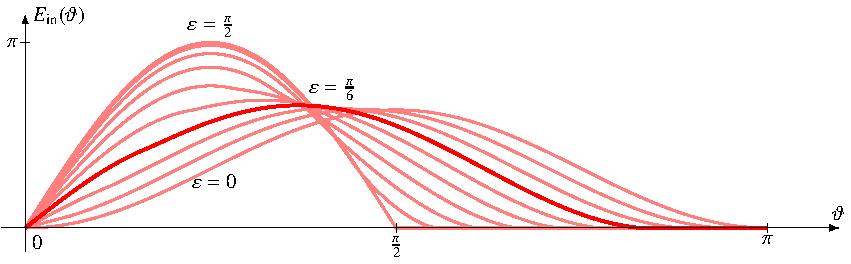
\includegraphics[width=\hsize]{chapters/5/ein1.pdf}
\caption{Strahlungsleistung auf geographischer Breite $\vartheta$,
gegeben durch Formel~\eqref{skript:einstrahlung:breite}.
\label{skript:einstrahlung:ein1}}
\end{figure}%
Die gesamte Strahlungsleistung auf dem Breitenkreis $\vartheta$
ist
\begin{equation}
E_{\text{in}}(\vartheta)
=
\varepsilon(\vartheta,\gamma)
\cdot
\sin\vartheta
\label{skript:einstrahlung:breite}
\end{equation}
Die resultierende Funktion ist in Abbildung~\ref{skript:einstrahlung:ein1}
dargestellt.

\subsection{Einstrahlung über ein Jahr}
\begin{figure}
\centering
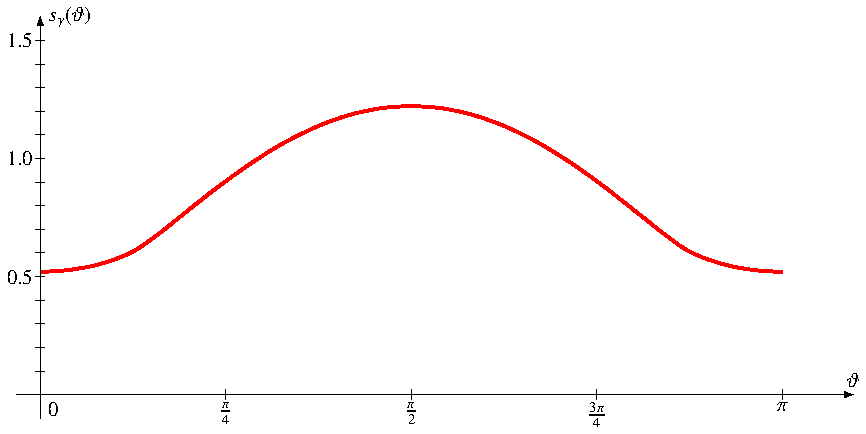
\includegraphics[width=\hsize]{chapters/5/total.pdf}
\caption{Einstrahlung über ein Jahr in Abhängigkeit von der geographischen
Breite.
\label{skript:einstrahlung:total}}
\end{figure}
Die in \eqref{skript:einstrahlung:breite} gefunden Einstrahlung auf einem
Breitengrad $\vartheta$ geht von einer konstanten Neigung der Erdachse aus.
Die Bewegung der Erde um die Sonne bedeutet aber, dass die Neigung der
der Erdachse scheinbar variert,
es gilt nämlich
\[
\tan \gamma(t) = \tan\gamma_\text{max}\cdot \sin t.
\]
Für ein Klimamodell wesentlich ist daher der Mittelwert
\[
s_{\gamma_\text{max}}(\vartheta)
=
\frac1{2\pi}
\int_0^{2\pi} \varepsilon(\vartheta,\gamma(t))\,dt
\]
von \eqref{skript:einstrahlung:breite} über ein Jahr.
Abbildung~\ref{skript:einstrahlung:total} zeigt das Resultat der 
numerischen Integration.










%
% bilanz.tex -- Bilanz-Modelle
%
% (c) 2018 Prof Dr Andreas Müller, Hochschule Rapperswil
%
\section{Strahlungsbilanzmodelle\label{skript:section:budyko}}
\rhead{Strahlunbsbilanzmodelle}
Im Kapitel~\ref{chapter:wetter und klima} haben wir die physikalischen
Grundlagen der Wetter und Klimaphänomene studiert.
In diesem Abschnitt wollen wir ein einfaches Modell für die Energiebilanz
der Erde entwickeln.

\subsection{Strahlungsbilanz\label{skript:subsection:strahlungsbilanz}}
Wir formulieren ein Modell mit einer einzigen Variablen, der globalen
Mitteltemperatur $T$.
Berechnet werden soll die zeitliche Entwicklung von $T$.

\subsubsection{Einstrahlung}
Die Erde mit Radius $R$ erhält ihre Energie von der Sonne, die
den konstanten Energiefluss $S_0 = 1368 \text{W\,m}^{-2}$
einstrahlt.
Der Querschnitt der Erde ist $\pi R^2$, auf den eine Leistung von
$\pi R^2 S_0$ fällt.
Die Atmosphäre und die Weltmeere transportieren diese Energie, wir nehmen
an, sie gleichmässig über die ganze Erdoberfläche verteilt wird.
Die pro Flächeneinheit anfallende Leistung ist daher
\begin{equation}
\frac{\pi R^2 S_0}{4\pi R^2} = \frac14S_0=Q.
\label{skript:bilanz:einstrahlung}
\end{equation}

Doch kann nicht die gesamte Energie absorbiert werden.
Ein Teil wird von Wolken oder von Eis an der Oberfläche 
gleich wieder reflektiert, aber auch Landmassen und die Meere reflektieren
einen kleineren Teil der Strahlung.
Die auf Seite~\pageref{skript:subsubsection:albedo} beschriebene Albedo
hat für die Erde Werte zwischen $0.3$ und $0.7$ je nach dem Grad der
Bewölkung und der Vereisung.
Bei tieferer Temperatur muss mit stärkerer Vereisung und mehr Wolken
gerechnet werden.
Sei $\alpha(T)$ die Albedo der Erde bei der Temperatur $T$.
Der von der Erde absorbierte Fluss ist daher
\begin{equation}
(1-\alpha(T)) Q.
\label{skript:bilanz:ausstrahlung}
\end{equation}
Die Grösse $1-\alpha(T)$ heisst auch die {\em Coalbedo}.
\index{Coalbedo}%

\subsubsection{Ausstrahlung}
Die Erde verliert Energie auch wieder durch Strahlung.
Nach dem Stefan-Boltzmannschen Gesetz~\eqref{skript:stefon-boltzmann}
ist die Ausstrahlung der Erde proportional zur vierten Potenz der
Temperatur, also $T^4$.

\subsubsection{Bilanzgleichung}
Die Temperatur ändert sich umso mehr, je grösser das Ungleichgewicht
zwischen Einstrahlung \eqref{skript:bilanz:einstrahlung} und
\eqref{skript:bilanz:ausstrahlung} ist.
Die Wärmekapazität der Erdoberfläche spielt ebenfalls
eine Rolle, je grösser diese ist, desto träger folgt die Temperatur dem
Energiebilanzüberschuss.

Wir erhalten so die Differentialgleichung
\begin{equation}
C\frac{dT}{dt}
=
(1-\alpha(T)) Q - \sigma T^4.
\label{skript:bilanz:basic}
\end{equation}
Je grösser $C$ ist, desto kleiner ist die Änderungsgeschwindigkeit der
globalen Mitteltemperatur bei gleicher rechter Seite.

\subsubsection{Gleichgewichtslösung}
Wir suchen eine Gleichgewichtslösung für dieses Modell, und nehmen zu diesem
Zweck den typischen Wert $\alpha=0.3$ der Albedo der Erde.
Sie muss $\dot T=0$ erfüllen, also
\begin{align*}
(1-\alpha) Q -\sigma T^4 &=0
\\
\Rightarrow
\qquad
T&=\root 4\of{\frac{(1-\alpha)Q}{\sigma}}
\end{align*}
Setzt man die üblichen Werte für $Q$ ein, erhält man eine globale
Mitteltemperatur von $T=254.8\,\text{K}$.

\subsubsection{Treibhauseffekt}
Die tatsächliche global Mitteltemperatur $T=287.7\,\text{K}$ ist.
Diese Diskrepanz ist zwei Unzulänglichkeiten diesen einfachen
Modells zurückzuführen:
\begin{enumerate}
\item
Der Treibhauseffekt sorgt dafür, dass nur ein Teil der abgestrahlten
Wärmestrahlung die Erde tatsächlich verlässt.
Wir können dies dadurch modellieren, dass wir in der Gleichung
\eqref{skript:bilanz:basic} den Ausstrahlungsterm um einen Faktor
$\varepsilon$ reduzieren, der den Treibhauseffekt modellieren soll.
Die neue Grundgleichung wird dann
\begin{equation}
C\frac{dT}{dt}
=
(1-\alpha(T)) Q - \varepsilon\sigma T^4.
\label{skript:bilanz:basic2}
\end{equation}
Um die aktuelle Gleichgewichtstemperatur $T=287.7\,\text{K}$ von 2010
zu reproduzieren müssen wir $\varepsilon=0.32$ wählen.
\item
Die Albedo hängt von der Temperatur ab und wird mit abnehmender 
Temperatur grösser.
Bei sehr tiefen Temperaturen kann die Albedo auf bis $0.7$ steigen.
Ein einfaches Modell, welches Diesen Sachverhalt abbildet, ist
\begin{equation}
\alpha(T)=0.5-0.2\tanh\biggl(\frac{T-265}{10}\biggr)
\label{skript:bilanz:albedo}
\end{equation}
\end{enumerate}

\subsubsection{Gleichgewichte}
\begin{figure}
\centering
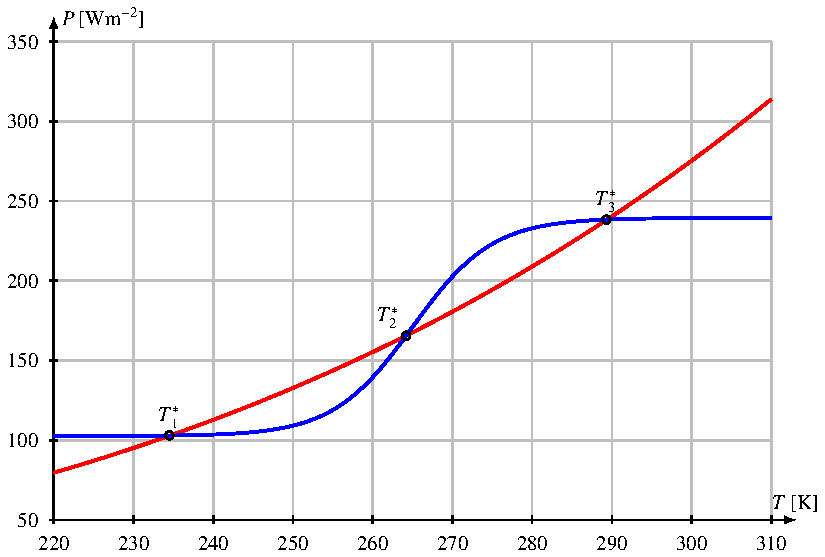
\includegraphics{chapters/5/bilanzmodell.pdf}
\caption{Einstrahlung und Ausstrahlung in dem einfachen Bilanzmodell
mit der Modellgleichung
\eqref{skript:bilanz:basic2} und der Albedo-Funktion
\eqref{skript:bilanz:albedo}.
Die Ausstrahlung $\varepsilon\sigma T^4$ ist rot eingezeichnet,
blau ist die Ausstrahlung.
Es entstehen drei Gleichgewichtspunkte $T_1^*$, $T_2^2*$ und $T_3^*$,
von denen aber $T_2^*$ nicht stabil ist.
\label{skript:bilanz:modellbild}}
\end{figure}
Das Modell mit der Albedo-Funktion~\eqref{skript:bilanz:albedo}
hat nicht nur einen sondern drei Gleichgewichtspunkte.
Die Einstrahlung und die Ausstrahlung ist in
Abbildung~\ref{skript:bilanz:modellbild} dargestellt.

Die beiden Gleichgewichtspunkte $T_1^*$ und $T_3^*$ sind stabil.
In beiden Punkten ändert sich die absorbierte Energie kaum bei
einer Temperaturänderung, aber die Ausstrahlung wird bei erhöhter 
Temperatur wesentlich effizienter, so dass sich die Erde wieder
abkühlt.
Ebenso verringert sich die Ausstrahlung bei leicht tieferer Temperatur
sofort, so dass die Erde sich wieder zur Gleichgewichtstemperatur aufwärmen
kann.

Das Gleichgewicht $T_2^*$ ist dagegen nicht stabil.
Bei höherer Temperatur wird die Einstrahlung sofort grösser, ohne dass
die Ausstrahlung mithalten kann, so dass sich die Erde weiter
aufwärmt bis zur Temperatur $T_3^*$.
Bei leicht tieferer Temperatur steigt die Albedo stark an so dass die
Einstrahlung schnell abnimmt, während die Ausstrahlung nur vergleichsweise
langsam zurückgeht, die Erde kühlt sich bis auf die Temperatur $T_1^*$ ab.

\subsubsection{Bifurkation und globale Erwärmung}
\begin{figure}
\centering
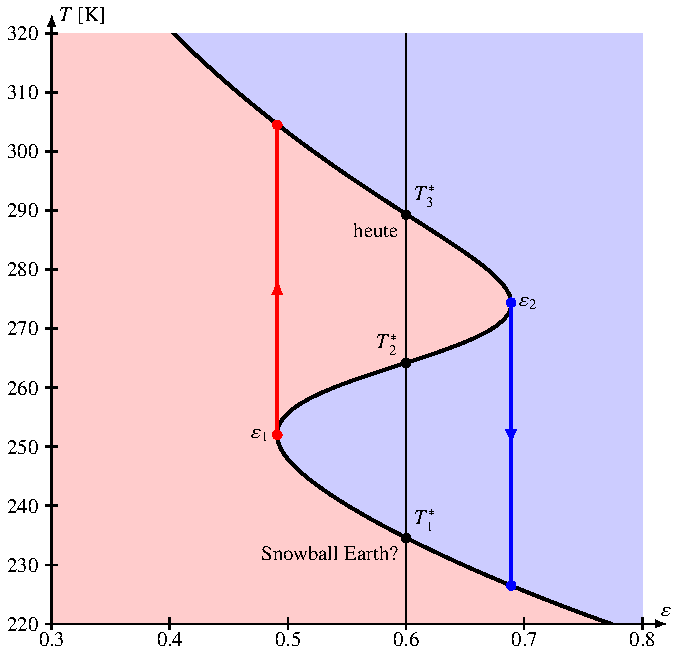
\includegraphics{chapters/5/bifurkation.pdf}
\caption{Bifurkationsdiagramm für das Bilanzmodell
\eqref{skript:bilanz:basic2}
in Abhängigkeit vom Treibhauseffekt-Parameter $\varepsilon$.
\label{skript:bilanz:bifurkation}}
\end{figure}
Der Parameter $\varepsilon$ modelliert den Treibhauseffekt.
Steigt die Konzentration der Klimagase in der Atmosphäre, wird die
abgestrahlten Leistung geringer, also $\varepsilon$ kleiner.
Es lohnt sich daher, die Entwicklung des Gleichgewichtspunkte in 
Abhängigkeit von $\varepsilon$ zu untersuchen.
Das Bifurkationsdiagramm des Modells
\eqref{skript:bilanz:basic2} in Abhängigkeit von $\varepsilon$
ist in Abbildung~\ref{skript:bilanz:bifurkation} dargestellt.

Man kann aus dem Diagramm ablesen, dass mit weitterer Zunahme des 
Treibhauseffektes, als mit Abnahme von $\varepsilon$, die globale
Mitteltemperatur weiter ansteigen wird.
Sinkt $\varepsilon$ unter den kritischen Wert $\varepsilon_1$ steigt die
Temperatur auf über $305\,\text{K}$.
In diesem Fall verschwinden die beiden Gleichgewichtspunkte $T_1^*$
und $T_2^*$, es bleibt nur das Gleichgewicht $T_3^*$.

Interessant ist aber auch, was bei starker Abnahme der
Treibhausgaskonzentration passiert.
Wenn $\varepsilon$ über $\varepsilon_2$ ansteigt, dann verschwinde
$T_3^*$ und $T_2^*$, es bleibt nur der Gleichgewichtspunkt $T_1^*$,
bei dem die ganze auf sehr tiefer Temperatur vereist.
Man vermutet, dass genau dieser Zustand in der Phase des {\em Snowball Earth}
eingetreten ist, als die ersten photosynthetisierenden Organismen die
Treibhausgase dramatische reduziert und damit $\varepsilon$ stark
erhöht hatten.
Man beachte dass es nur möglich ist, den heutigen Zustand wieder zu 
erreichen, indem die Treibhausgaskonzentration soweit gesteigert
wird, dass $\varepsilon<\varepsilon_1$ wird.
Es muss im Laufe der Erdgeschichte also nach der Snowball Earth Phase
auch Phasen mit wesentlich höherer Treibhausgaskonzentration als heute
gegeben haben.

\subsection{Modell von Budyko\label{subsection:modell von budyko}}
Bisher haben wir die Ausstrahlung mit Hilfe des Stefan-Boltzmannschen
Gesetzes für die Strahlung eines schwarzen Körpers modelliert.
Es ist fraglich, ob dies tatsächlich zutreffend ist.
Die Ausstrahlung $E_\text{out}(T)$ der Ausstrahlung könnte also durchaus
eine kompliziertere Funktion sein.
Sie muss aber so beschaffen sein, dass sich bei der aktuellen
Mitteltemperatur $T^*$ ein stabiles Gleichgewicht ergibt.
In der Umgebung des Gleichgewichtes kann die Funktion $E_\text{out}(T)$
als lineare Funktion
$E_\text{out}= A+BT$
dargestellt werden.
Nahe bei $T^*$ kann die globale Mitteltemperatur also mit einem Modell
der Form
\begin{equation}
C
\frac{dT}{dt}
=
(1-\alpha(T)) Q- (A+BT)
\end{equation}
beschrieben werden.
Das Gleichgewicht erfüllt
\[
(1-\alpha(T^*))Q=A+BT^*
\] 
und ist stabil, wenn die Steigung der Einstrahlung kleiner ist als die
Die Steigung der Ausstrahlung, also
\begin{equation}
-Q\alpha'(T)
<
B.
\label{skript:budyko:cond}
\end{equation}
Dieses Modell wurde schon in den sechziger Jahren von Budyko vorgeschlagen.
Zahlenwerte für $A$ und $B$ konnte seit der damaligen Zeit durch
Satellitenmessungen bestimmt werden.

Die Folgen des Treibhauseffektes sind auch in diesem einfacheren Modell
nachvollziehbar.
Die Erhöhung der Treibhausgaskonzentration reduziert die Ausstrahlung,
was sich zum Beispiel in einem kleineren Wert von $B$ äussert.
Eine Abnahme von $B$ um $\Delta B$ führt zu einer
Änderung der Gleichgewichtstemperatur um $\Delta T$, die die Gleichung
\begin{align*}
(1-\alpha(T^*+\Delta T))Q
&=
A + (B-\Delta B)(T^*+\Delta T)
\\
\underbrace{(1-\alpha(T^*))Q}_{\displaystyle=A+BT^*}
-Q\alpha'(T^*)\Delta T
&=
A+BT^*
- T^*\Delta B
+B\Delta T
\\
(Q\alpha'(T^*)
+
B)\Delta T
&=
T^*
\Delta B
\\
\Delta T
&=
\frac{T^*\Delta B}{Q\alpha'(T^*)+B}
\end{align*}
erfüllt.
Man kann daraus ablesen, dass eine Abnahme von $B$ genau dann zu einer
Zunahme der Mitteltemperatur, wenn der Nenner positiv ist, also
\[
Q\alpha'(T^*)+B > 0
\qquad\Rightarrow\qquad
-Q\alpha'(T^*)<B,
\]
was die Bedingung
\eqref{skript:budyko:cond}
beweist.





%
% zonen.tex -- Zonenmodelle für das Klima
%
% (c) 2018 Prof Dr Andreas Müller, Hochschule Rapperswil
%
\chapter{Zonenmodelle\label{chapter:zonenmodelle}}
\lhead{Kapitel \thechapter: Zonenmodelle}
Die Erdrotation ist schnell im Vergleich zu den für typische Klimamodelle
wesentlichen Zeitspannen.
Wesentliche Aspekte der Klimaentwicklung sollten sich daher immer
noch modellieren lassen, wenn man den Zustand des Klimasystems über
die Erdrotation mittelt.
In diesem Kapitel werden daher vereinfachte Modelle diskutiert,
die nur die geographischen Länge als geometrischen Parameter haben.

%
% strahlung.tex
%
% (c) 2018 Prof Dr Andreas Müller, Hochschule Rapperswil
%
\section{Strahlung\label{section:strahlung}}
\rhead{Strahlung}
Die von der Erde empfange Strahlung sowie die Albedo wurden bereits in
Abschnitt~\ref{skript:grundlagen:strahlung} untersucht.
Für die später in diesem Kapitel zu untersuchenden Modelle ist aber
erforderlich, die örtliche Verteilung der Strahlung auf der Erdoberfläche
genauer zu verstehen.
In diesem Abschnitt wird daher zuerst die Strahlungsleistung auf einer
Halbkugel und später auf einer Zone um einen Breitenkreis berechnet.
\input{chapters/5/halbkugel.tex}
\input{chapters/5/einstrahlung.tex}

%
% bilanz.tex -- Bilanz-Modelle
%
% (c) 2018 Prof Dr Andreas Müller, Hochschule Rapperswil
%
\section{Strahlungsbilanzmodelle\label{skript:section:budyko}}
\rhead{Strahlunbsbilanzmodelle}
Im Kapitel~\ref{chapter:wetter und klima} haben wir die physikalischen
Grundlagen der Wetter und Klimaphänomene studiert.
In diesem Abschnitt wollen wir ein einfaches Modell für die Energiebilanz
der Erde entwickeln.

\subsection{Strahlungsbilanz\label{skript:subsection:strahlungsbilanz}}
Wir formulieren ein Modell mit einer einzigen Variablen, der globalen
Mitteltemperatur $T$.
Berechnet werden soll die zeitliche Entwicklung von $T$.

\subsubsection{Einstrahlung}
Die Erde mit Radius $R$ erhält ihre Energie von der Sonne, die
den konstanten Energiefluss $S_0 = 1368 \text{W\,m}^{-2}$
einstrahlt.
Der Querschnitt der Erde ist $\pi R^2$, auf den eine Leistung von
$\pi R^2 S_0$ fällt.
Die Atmosphäre und die Weltmeere transportieren diese Energie, wir nehmen
an, sie gleichmässig über die ganze Erdoberfläche verteilt wird.
Die pro Flächeneinheit anfallende Leistung ist daher
\begin{equation}
\frac{\pi R^2 S_0}{4\pi R^2} = \frac14S_0=Q.
\label{skript:bilanz:einstrahlung}
\end{equation}

Doch kann nicht die gesamte Energie absorbiert werden.
Ein Teil wird von Wolken oder von Eis an der Oberfläche 
gleich wieder reflektiert, aber auch Landmassen und die Meere reflektieren
einen kleineren Teil der Strahlung.
Die auf Seite~\pageref{skript:subsubsection:albedo} beschriebene Albedo
hat für die Erde Werte zwischen $0.3$ und $0.7$ je nach dem Grad der
Bewölkung und der Vereisung.
Bei tieferer Temperatur muss mit stärkerer Vereisung und mehr Wolken
gerechnet werden.
Sei $\alpha(T)$ die Albedo der Erde bei der Temperatur $T$.
Der von der Erde absorbierte Fluss ist daher
\begin{equation}
(1-\alpha(T)) Q.
\label{skript:bilanz:ausstrahlung}
\end{equation}
Die Grösse $1-\alpha(T)$ heisst auch die {\em Coalbedo}.
\index{Coalbedo}%

\subsubsection{Ausstrahlung}
Die Erde verliert Energie auch wieder durch Strahlung.
Nach dem Stefan-Boltzmannschen Gesetz~\eqref{skript:stefon-boltzmann}
ist die Ausstrahlung der Erde proportional zur vierten Potenz der
Temperatur, also $T^4$.

\subsubsection{Bilanzgleichung}
Die Temperatur ändert sich umso mehr, je grösser das Ungleichgewicht
zwischen Einstrahlung \eqref{skript:bilanz:einstrahlung} und
\eqref{skript:bilanz:ausstrahlung} ist.
Die Wärmekapazität der Erdoberfläche spielt ebenfalls
eine Rolle, je grösser diese ist, desto träger folgt die Temperatur dem
Energiebilanzüberschuss.

Wir erhalten so die Differentialgleichung
\begin{equation}
C\frac{dT}{dt}
=
(1-\alpha(T)) Q - \sigma T^4.
\label{skript:bilanz:basic}
\end{equation}
Je grösser $C$ ist, desto kleiner ist die Änderungsgeschwindigkeit der
globalen Mitteltemperatur bei gleicher rechter Seite.

\subsubsection{Gleichgewichtslösung}
Wir suchen eine Gleichgewichtslösung für dieses Modell, und nehmen zu diesem
Zweck den typischen Wert $\alpha=0.3$ der Albedo der Erde.
Sie muss $\dot T=0$ erfüllen, also
\begin{align*}
(1-\alpha) Q -\sigma T^4 &=0
\\
\Rightarrow
\qquad
T&=\root 4\of{\frac{(1-\alpha)Q}{\sigma}}
\end{align*}
Setzt man die üblichen Werte für $Q$ ein, erhält man eine globale
Mitteltemperatur von $T=254.8\,\text{K}$.

\subsubsection{Treibhauseffekt}
Die tatsächliche global Mitteltemperatur $T=287.7\,\text{K}$ ist.
Diese Diskrepanz ist zwei Unzulänglichkeiten diesen einfachen
Modells zurückzuführen:
\begin{enumerate}
\item
Der Treibhauseffekt sorgt dafür, dass nur ein Teil der abgestrahlten
Wärmestrahlung die Erde tatsächlich verlässt.
Wir können dies dadurch modellieren, dass wir in der Gleichung
\eqref{skript:bilanz:basic} den Ausstrahlungsterm um einen Faktor
$\varepsilon$ reduzieren, der den Treibhauseffekt modellieren soll.
Die neue Grundgleichung wird dann
\begin{equation}
C\frac{dT}{dt}
=
(1-\alpha(T)) Q - \varepsilon\sigma T^4.
\label{skript:bilanz:basic2}
\end{equation}
Um die aktuelle Gleichgewichtstemperatur $T=287.7\,\text{K}$ von 2010
zu reproduzieren müssen wir $\varepsilon=0.32$ wählen.
\item
Die Albedo hängt von der Temperatur ab und wird mit abnehmender 
Temperatur grösser.
Bei sehr tiefen Temperaturen kann die Albedo auf bis $0.7$ steigen.
Ein einfaches Modell, welches Diesen Sachverhalt abbildet, ist
\begin{equation}
\alpha(T)=0.5-0.2\tanh\biggl(\frac{T-265}{10}\biggr)
\label{skript:bilanz:albedo}
\end{equation}
\end{enumerate}

\subsubsection{Gleichgewichte}
\begin{figure}
\centering
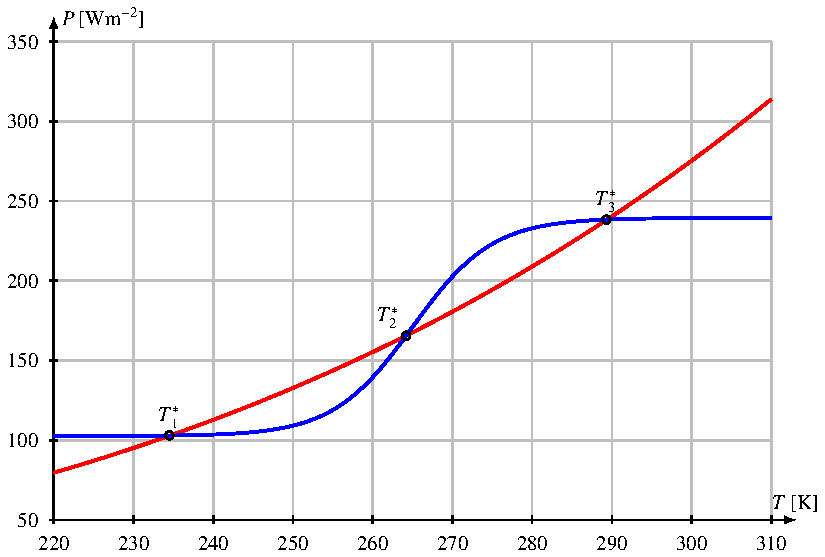
\includegraphics{chapters/5/bilanzmodell.pdf}
\caption{Einstrahlung und Ausstrahlung in dem einfachen Bilanzmodell
mit der Modellgleichung
\eqref{skript:bilanz:basic2} und der Albedo-Funktion
\eqref{skript:bilanz:albedo}.
Die Ausstrahlung $\varepsilon\sigma T^4$ ist rot eingezeichnet,
blau ist die Ausstrahlung.
Es entstehen drei Gleichgewichtspunkte $T_1^*$, $T_2^2*$ und $T_3^*$,
von denen aber $T_2^*$ nicht stabil ist.
\label{skript:bilanz:modellbild}}
\end{figure}
Das Modell mit der Albedo-Funktion~\eqref{skript:bilanz:albedo}
hat nicht nur einen sondern drei Gleichgewichtspunkte.
Die Einstrahlung und die Ausstrahlung ist in
Abbildung~\ref{skript:bilanz:modellbild} dargestellt.

Die beiden Gleichgewichtspunkte $T_1^*$ und $T_3^*$ sind stabil.
In beiden Punkten ändert sich die absorbierte Energie kaum bei
einer Temperaturänderung, aber die Ausstrahlung wird bei erhöhter 
Temperatur wesentlich effizienter, so dass sich die Erde wieder
abkühlt.
Ebenso verringert sich die Ausstrahlung bei leicht tieferer Temperatur
sofort, so dass die Erde sich wieder zur Gleichgewichtstemperatur aufwärmen
kann.

Das Gleichgewicht $T_2^*$ ist dagegen nicht stabil.
Bei höherer Temperatur wird die Einstrahlung sofort grösser, ohne dass
die Ausstrahlung mithalten kann, so dass sich die Erde weiter
aufwärmt bis zur Temperatur $T_3^*$.
Bei leicht tieferer Temperatur steigt die Albedo stark an so dass die
Einstrahlung schnell abnimmt, während die Ausstrahlung nur vergleichsweise
langsam zurückgeht, die Erde kühlt sich bis auf die Temperatur $T_1^*$ ab.

\subsubsection{Bifurkation und globale Erwärmung}
\begin{figure}
\centering
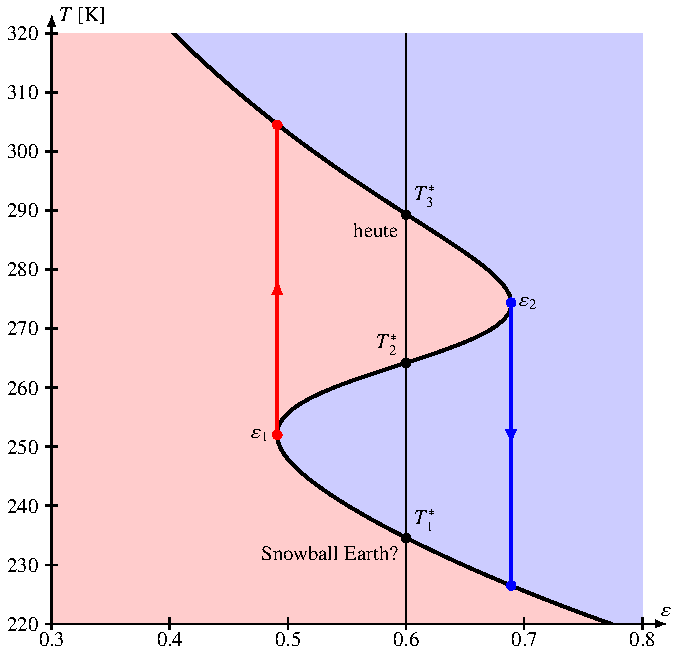
\includegraphics{chapters/5/bifurkation.pdf}
\caption{Bifurkationsdiagramm für das Bilanzmodell
\eqref{skript:bilanz:basic2}
in Abhängigkeit vom Treibhauseffekt-Parameter $\varepsilon$.
\label{skript:bilanz:bifurkation}}
\end{figure}
Der Parameter $\varepsilon$ modelliert den Treibhauseffekt.
Steigt die Konzentration der Klimagase in der Atmosphäre, wird die
abgestrahlten Leistung geringer, also $\varepsilon$ kleiner.
Es lohnt sich daher, die Entwicklung des Gleichgewichtspunkte in 
Abhängigkeit von $\varepsilon$ zu untersuchen.
Das Bifurkationsdiagramm des Modells
\eqref{skript:bilanz:basic2} in Abhängigkeit von $\varepsilon$
ist in Abbildung~\ref{skript:bilanz:bifurkation} dargestellt.

Man kann aus dem Diagramm ablesen, dass mit weitterer Zunahme des 
Treibhauseffektes, als mit Abnahme von $\varepsilon$, die globale
Mitteltemperatur weiter ansteigen wird.
Sinkt $\varepsilon$ unter den kritischen Wert $\varepsilon_1$ steigt die
Temperatur auf über $305\,\text{K}$.
In diesem Fall verschwinden die beiden Gleichgewichtspunkte $T_1^*$
und $T_2^*$, es bleibt nur das Gleichgewicht $T_3^*$.

Interessant ist aber auch, was bei starker Abnahme der
Treibhausgaskonzentration passiert.
Wenn $\varepsilon$ über $\varepsilon_2$ ansteigt, dann verschwinde
$T_3^*$ und $T_2^*$, es bleibt nur der Gleichgewichtspunkt $T_1^*$,
bei dem die ganze auf sehr tiefer Temperatur vereist.
Man vermutet, dass genau dieser Zustand in der Phase des {\em Snowball Earth}
eingetreten ist, als die ersten photosynthetisierenden Organismen die
Treibhausgase dramatische reduziert und damit $\varepsilon$ stark
erhöht hatten.
Man beachte dass es nur möglich ist, den heutigen Zustand wieder zu 
erreichen, indem die Treibhausgaskonzentration soweit gesteigert
wird, dass $\varepsilon<\varepsilon_1$ wird.
Es muss im Laufe der Erdgeschichte also nach der Snowball Earth Phase
auch Phasen mit wesentlich höherer Treibhausgaskonzentration als heute
gegeben haben.

\subsection{Modell von Budyko\label{subsection:modell von budyko}}
Bisher haben wir die Ausstrahlung mit Hilfe des Stefan-Boltzmannschen
Gesetzes für die Strahlung eines schwarzen Körpers modelliert.
Es ist fraglich, ob dies tatsächlich zutreffend ist.
Die Ausstrahlung $E_\text{out}(T)$ der Ausstrahlung könnte also durchaus
eine kompliziertere Funktion sein.
Sie muss aber so beschaffen sein, dass sich bei der aktuellen
Mitteltemperatur $T^*$ ein stabiles Gleichgewicht ergibt.
In der Umgebung des Gleichgewichtes kann die Funktion $E_\text{out}(T)$
als lineare Funktion
$E_\text{out}= A+BT$
dargestellt werden.
Nahe bei $T^*$ kann die globale Mitteltemperatur also mit einem Modell
der Form
\begin{equation}
C
\frac{dT}{dt}
=
(1-\alpha(T)) Q- (A+BT)
\end{equation}
beschrieben werden.
Das Gleichgewicht erfüllt
\[
(1-\alpha(T^*))Q=A+BT^*
\] 
und ist stabil, wenn die Steigung der Einstrahlung kleiner ist als die
Die Steigung der Ausstrahlung, also
\begin{equation}
-Q\alpha'(T)
<
B.
\label{skript:budyko:cond}
\end{equation}
Dieses Modell wurde schon in den sechziger Jahren von Budyko vorgeschlagen.
Zahlenwerte für $A$ und $B$ konnte seit der damaligen Zeit durch
Satellitenmessungen bestimmt werden.

Die Folgen des Treibhauseffektes sind auch in diesem einfacheren Modell
nachvollziehbar.
Die Erhöhung der Treibhausgaskonzentration reduziert die Ausstrahlung,
was sich zum Beispiel in einem kleineren Wert von $B$ äussert.
Eine Abnahme von $B$ um $\Delta B$ führt zu einer
Änderung der Gleichgewichtstemperatur um $\Delta T$, die die Gleichung
\begin{align*}
(1-\alpha(T^*+\Delta T))Q
&=
A + (B-\Delta B)(T^*+\Delta T)
\\
\underbrace{(1-\alpha(T^*))Q}_{\displaystyle=A+BT^*}
-Q\alpha'(T^*)\Delta T
&=
A+BT^*
- T^*\Delta B
+B\Delta T
\\
(Q\alpha'(T^*)
+
B)\Delta T
&=
T^*
\Delta B
\\
\Delta T
&=
\frac{T^*\Delta B}{Q\alpha'(T^*)+B}
\end{align*}
erfüllt.
Man kann daraus ablesen, dass eine Abnahme von $B$ genau dann zu einer
Zunahme der Mitteltemperatur, wenn der Nenner positiv ist, also
\[
Q\alpha'(T^*)+B > 0
\qquad\Rightarrow\qquad
-Q\alpha'(T^*)<B,
\]
was die Bedingung
\eqref{skript:budyko:cond}
beweist.





%
% zonen.tex -- Zonenmodelle für das Klima
%
% (c) 2018 Prof Dr Andreas Müller, Hochschule Rapperswil
%
\chapter{Zonenmodelle\label{chapter:zonenmodelle}}
\lhead{Kapitel \thechapter: Zonenmodelle}
Die Erdrotation ist schnell im Vergleich zu den für typische Klimamodelle
wesentlichen Zeitspannen.
Wesentliche Aspekte der Klimaentwicklung sollten sich daher immer
noch modellieren lassen, wenn man den Zustand des Klimasystems über
die Erdrotation mittelt.
In diesem Kapitel werden daher vereinfachte Modelle diskutiert,
die nur die geographischen Länge als geometrischen Parameter haben.

\input{chapters/5/strahlung.tex}
\input{chapters/5/bilanz.tex}
\input{chapters/5/zonen.tex}
\input{chapters/5/spektral.tex}


%
% spektral.tex -- Einführung in spektrale Methoden
%
% (c) 2018 Prof Dr Andreas Müller, Hochschule Rapperswil
%
\section{Spektrale Methoden\label{section:spektrale methoden}}
\rhead{Spektrale Methoden}
In den Ausführungen zum Lorenz-Modell in Abschnitt~\ref{section:lorenz-modell}
werden wir sehen,
wie man mit Hilfe einer geeigneten Wahl von Basisfunktionen
die komplexen fluiddynamischen partiellen Differentialgleichungen zu einem
System von gewöhnlichen Differentialgleichungen vereinfachen kann.
Die Basis wurde so gewählt, dass einerseits möglichst viel geometrische
Information, im speziellen Fall die rechteckige Form des Definitionsgebietes,
bereits darin einfliesst.
Andererseits sollen sich die wesentlichsten Eigenschaften der Lösung bereits
aus wenigen Basisfunktionen rekonstruieren lassen.
Wie Kapitel~\ref{chapter:lorenz2} zeigt, lässt sich die Idee von
Abschnitt~\ref{section:lorenz-modell} sogar maschinell in eine
immer genaueres Modell erweitern, wenn nur eine geeignete Menge
von Basisfunktionen gefunden werden kann.
Ziel diese Abschnittes ist zu illustrieren, wie so eine Basis von
Funktionen aussehen könnte, mit der man globale Modelle vereinfachen
könnte.

\input{chapters/5/kugelkoordinaten.tex}
\input{chapters/5/kugelfunktionen.tex}
\input{chapters/5/spektralegleichungen.tex}





%
% spektral.tex -- Einführung in spektrale Methoden
%
% (c) 2018 Prof Dr Andreas Müller, Hochschule Rapperswil
%
\section{Spektrale Methoden\label{section:spektrale methoden}}
\rhead{Spektrale Methoden}
In den Ausführungen zum Lorenz-Modell in Abschnitt~\ref{section:lorenz-modell}
werden wir sehen,
wie man mit Hilfe einer geeigneten Wahl von Basisfunktionen
die komplexen fluiddynamischen partiellen Differentialgleichungen zu einem
System von gewöhnlichen Differentialgleichungen vereinfachen kann.
Die Basis wurde so gewählt, dass einerseits möglichst viel geometrische
Information, im speziellen Fall die rechteckige Form des Definitionsgebietes,
bereits darin einfliesst.
Andererseits sollen sich die wesentlichsten Eigenschaften der Lösung bereits
aus wenigen Basisfunktionen rekonstruieren lassen.
Wie Kapitel~\ref{chapter:lorenz2} zeigt, lässt sich die Idee von
Abschnitt~\ref{section:lorenz-modell} sogar maschinell in eine
immer genaueres Modell erweitern, wenn nur eine geeignete Menge
von Basisfunktionen gefunden werden kann.
Ziel diese Abschnittes ist zu illustrieren, wie so eine Basis von
Funktionen aussehen könnte, mit der man globale Modelle vereinfachen
könnte.

%
% kugelkoordinaten.tex -- Kugelkoordinaten
%
% (c) 2018 Prof Dr Andreas Müller, Hochschule Rapperswil
%

\subsection{Kugelkoordinaten}
Spektrale Methoden verwenden auf entscheidende Art und Weise die
Besonderheiten des natürlichen Koordinatensystems auf der Kugeloberfläche.
In diesem Abschnitt sollen daher Kugelkoordinaten und die zugehörigen 
Differentialoperatoren genauer untersucht werden.

\subsubsection{Koordinatenumrechnung}
\index{Kugelkoordinaten}%
Wir verwenden in diesem Abschnitt Kugelkoordinaten mit der üblichen
Konvention, dass die geographische Breite als Winkel $\vartheta$
ausgehend vom Nordpol oder der $z$-Achse gemessen wird,
dass also $\vartheta\in[0,\pi]$.
Die geographische Breite wird ausgehen von der $x$-Achse als
Winkel $\varphi$ gemessen.
Schliesslich bezeichnet $r$ die Entfernung eines Punktes vom Nullpunkt.

Ein Breitenkreis zur geographischen Breite $\vartheta$ hat Radius
$r\sin\vartheta$.
Damit ergeben sich die Formeln
\begin{align*}
x
&=
r\sin\vartheta\cos\varphi
\\
y
&=
r\sin\vartheta\sin\varphi
\\
z
&=
r\cos\vartheta
\end{align*}
für die Umrechnung von Kugelkoordinaten in kartesische Koordinaten.
\index{Umrechnungsformel!Kugel-Koordinaten in kartesische Koordinaten}%

\subsubsection{Differentialoperatoren}
Das Ziel ist, den Laplace-Operator in Kugelkoordinaten auszudrücken.
Zu diesem Zweck müssen die partiellen Ableitungsoperatoren nach den
Koordinaten $x$, $y$ und $z$ durch die Operatoren
\[
\frac{\partial}{\partial r},
\;
\frac{\partial}{\partial\vartheta}
\quad\text{und}\quad
\frac{\partial}{\partial\varphi}
\]
ausgedrückt werden.

Für die Ableitungsoperatoren gilt die Kettenregel in der Form
\begin{equation}
\begin{aligned}
\frac{\partial}{\partial x}
&=
\frac{\partial r}{\partial x}\frac{\partial}{\partial r}
+
\frac{\partial\vartheta}{\partial x}\frac{\partial}{\partial\vartheta}
+
\frac{\partial\varphi}{\partial x}\frac{\partial}{\partial\varphi},
\\
\frac{\partial}{\partial y}
&=
\frac{\partial r}{\partial y}\frac{\partial}{\partial r}
+
\frac{\partial\vartheta}{\partial y}\frac{\partial}{\partial\vartheta}
+
\frac{\partial\varphi}{\partial y}\frac{\partial}{\partial\varphi},
\\
\frac{\partial}{\partial z}
&=
\frac{\partial r}{\partial z}\frac{\partial}{\partial r}
+
\frac{\partial\vartheta}{\partial z}\frac{\partial}{\partial\vartheta}
+
\frac{\partial\varphi}{\partial z}\frac{\partial}{\partial\varphi}.
\end{aligned}
\label{skript:kugel:kettenregel}
\end{equation}
Die gesuchte Darstellung der Ableitungsoperatoren läuft also darauf
hinaus, die Ableitungen von Kugelkoordinaten nach nach kartesischen
Koordinaten zu bestimmen.

Die Ableitungen von $r$ werden einfacher zur berechnen durch die
Beziehung
\[
\frac{\partial r^2}{\partial x}
=
2r\frac{\partial r}{\partial x}
\qquad\Rightarrow\qquad
\frac{\partial r}{\partial x}
=\frac1{2r}\frac{\partial r^2}{\partial x}.
\]
Da $r^2=x^2+y^2+z^2$ folgt
\begin{equation}
\begin{aligned}
\frac{\partial r}{\partial x}
&=
\frac1{2r}\frac{\partial}{\partial x}(x^2+y^2+z^2)
=
\frac1{2r}2x
=
\frac{x}{r}
=
\sin\vartheta\cos\varphi,
\\
\frac{\partial r}{\partial y}
&=
\frac1{2r}\frac{\partial}{\partial x}(x^2+y^2+z^2)
=
\frac1{2r}2y
=
\frac{y}{r}
=
\sin\vartheta\sin\varphi
\\
\text{und}
\qquad
\frac{\partial r}{\partial z}
&=
\frac1{2r}\frac{\partial}{\partial z}(x^2+y^2+z^2)
=
\frac1{2r}2z
=
\frac{z}{r}
=
\cos\vartheta.
\end{aligned}
\label{skript:kugel:rableitungen}
\end{equation}

Auf ähnliche Weise lassen sich die Ableitungen von $\vartheta$ bestimmen.
Dazu geht man aus von der Identität $z=r\cos\vartheta$ und leitet sie
nach den kartesischen Koordinaten ab:
\begin{align*}
0
=
\frac{\partial z}{\partial x}
&=
\frac{\partial r}{\partial x}\cos\vartheta
-
r\sin\vartheta\frac{\partial \vartheta}{\partial x}
&&\Rightarrow&
\frac{\partial\vartheta}{\partial x}
&=
\frac{1}{r\sin\vartheta}
\cos\vartheta
\frac{\partial r}{\partial x},
\\
0
=
\frac{\partial z}{\partial y}
&=
\frac{\partial r}{\partial y}\cos\vartheta
-
r\sin\vartheta\frac{\partial \vartheta}{\partial y}
&&\Rightarrow&
\frac{\partial \vartheta}{\partial y}
&=
\frac{1}{r\sin\vartheta}
\cos\vartheta
\frac{\partial r}{\partial y},
\\
1
=
\frac{\partial z}{\partial z}
&=
\frac{\partial r}{\partial y}\cos\vartheta
-
r\sin\vartheta\frac{\partial \vartheta}{\partial y}
&&\Rightarrow&
\frac{\partial\vartheta}{\partial y}
&=
-\frac1{r\sin\vartheta}
\biggl(1-
\cos\vartheta
\frac{\partial r}{\partial z}
\biggr).
\end{align*}
Die Ableitungen von $r$ wurden in \eqref{skript:kugel:rableitungen}
bereits berechnet, so dass wir nach den
Ableitungen von $\vartheta$ auflösen können.
Wir erhalten
\begin{equation}
\begin{aligned}
\frac{\partial\vartheta}{\partial x}
&=
\frac1{r\sin\vartheta} \cos\vartheta \sin\vartheta\cos\varphi
=
\frac{\cos\vartheta\cos\varphi}{r},
\\
\frac{\partial\vartheta}{\partial y}
&=
\frac{1}{r\sin\vartheta} \cos\vartheta \sin\vartheta\sin\varphi
=
\frac{\cos\vartheta\sin\varphi}{r},
\\
\frac{\partial\vartheta}{\partial z}
&=
-\frac{1}{r\sin\vartheta}\underbrace{(1-\cos^2\vartheta)}_{\displaystyle\sin^2\vartheta}
=
-
\frac{\sin\vartheta}r.
\end{aligned}
\label{skript:kugel:thetaableitungen}
\end{equation}
Diese Umformungen waren möglich, weil $z$ nur von $r$ und $\vartheta$ abhing.
Die Kettenregel hat dann eine Beziehung zwischen den beiden Ableitungen
dieser Variablen geliefert.

Die verbleibenden Anleitungen können auf ähnliche Weise aus dem Ausdruck
$x=r\sin\vartheta\cos\varphi$
oder
$y=r\sin\vartheta\sin\varphi$
gewonnen werden.
Wenn man ihn partiell nach kartesischen Koordinaten ableitet,
steht auf der linken Seite eine 1 oder 0,
auf der rechten Seite ein Ausdruck mit allen drei Ableitungen von
Kugelkoordinaten nach $x$, wovon die Ableitungen von $r$ und $\vartheta$
nach den kartesischen Koordinaten bereits bekannt sind.
Man kann also nach den Ableitungen von $\varphi$ auflösen.
Die etwas mühsame Berechnung liefert
\begin{equation}
\begin{aligned}
\frac{\partial \varphi}{\partial x}
&=
-\frac{\sin\varphi}{r\sin\vartheta},
\\
\frac{\partial \varphi}{\partial y}
&=
\frac{\cos\varphi}{r\sin\vartheta},
\\
\frac{\partial \varphi}{\partial z}
&=
0.
\end{aligned}
\label{skript:kugel:phiableitungen}
\end{equation}

In den Gleichungen
\eqref{skript:kugel:rableitungen},
\eqref{skript:kugel:thetaableitungen}
und
\eqref{skript:kugel:phiableitungen}
haben wir alle Koeffizienten für die Kettenregel
\eqref{skript:kugel:kettenregel}
gefunden.
Zusammen erlauben sie, Ableitungen nach kartesischen Koordinaten
durch Ableitungen nach Kugelkoordinaten auszudrücken.

\subsubsection{Laplace-Operator}
In kartesischen Koordinaten ist der Laplace-Operator gegeben durch die
Definition
\[
\Delta
=
\frac{\partial^2}{\partial x^2}
+
\frac{\partial^2}{\partial y^2}
+
\frac{\partial^2}{\partial z^2}.
\]
Durch Einsetzen der Ableitungsoperatoren nach
\eqref{skript:kugel:kettenregel} unter Verwendung der Gleichungen
\eqref{skript:kugel:rableitungen},
\eqref{skript:kugel:thetaableitungen}
und
\eqref{skript:kugel:phiableitungen}
kann man nach ziemlich langwieriger
Rechnung~\cite[Anhang B.3]{skript:mathsem-qm}
den Ausdruck
\begin{equation}
\Delta
=
\frac1{r^2}\frac{\partial}{\partial r}
\biggl(r^2\frac{\partial}{\partial r}\biggr)
+
\frac{1}{r^2\sin\vartheta}\frac{\partial}{\partial\vartheta}
\biggl(\sin\vartheta\frac{\partial}{\partial\vartheta}\biggr)
+
\frac{1}{r^2}
\frac{1}{\sin^2\vartheta}
\frac{\partial^2}{\partial\varphi^2}.
\end{equation}
für den Laplace-Operator in Kugelkoordinaten finden.
\index{Laplace-Operator in Kugelkoordinaten}%


%
% kugelfunktionen.tex -- Kugelfunktionen
%
% (c) 2018 Prof Dr Andreas Müller, Hochschule Rapperswil
%
\subsection{Kugelfunktionen}
Die Basisfunktionen im Lorenz-Modell waren aus zwei Gründen besonders
erfolgreich.
\begin{enumerate}
\item
Die Basisfunktionen waren Produkte von Funktionen, die jeweils nur von
einer Koordinate abhängen.
In einem Produkt 
$f(x,y)=X(x)\cdot Y(y)$ 
sind die Ableitungen nach den Koordinaten besonders einfach auszurechnen,
da gilt
\[
\begin{aligned}
\frac{\partial f}{\partial x}(x,y) &= X'(x)\cdot Y(y)
&&\text{und}&
\frac{\partial f}{\partial y}(x,y) &= X(x)\cdot Y'(y).
\end{aligned}
\]
\item
Die Basisfunktionen waren Eigenfunktionen des Laplace-Operators, also
\[
\Delta f = \lambda f.
\]
Da in den Gleichungen der Strömungsdynamik der Laplace-Operator
prominent vorkommt, bedeutet diese Eigenschaft, dass die Wirkung des
Laplace-Operators auf die Basisfunktionen durch Multiplikation mit
dem Eigenwert ersetzt werden kann.
Dadurch werden die Gleichungen sehr vereinfacht und die Ordnung
der Differentialgleichung reduziert sich.
\end{enumerate}
Wenn der Erfolg der speziellen Basiswahl im Lorenz-System für ein
Wetter- oder Klimamodell auf der Kugeloberfläche repliziert werden
soll, dann ist nahe liegend, dass dazu Funktionen mit den gleichen
Eigenschaften in Kugelkoordinaten gefunden werden müssen.

\subsubsection{Separationsansatz}
Die Produkteigenschaft bedeutet, dass die Basisfunktionen in der Form
\[
f(r,\varphi,\vartheta)
=
R(r)\cdot \Phi(\varphi)\cdot \Theta(\vartheta)
\]
gefunden werden müssen.
Das in Abschnitt~\ref{section:pdeloesungen} dargestellte
Separationsverfahren für partielle
Differentialgleichungen~\cite[Chapter 4]{skript:pde}
basiert genau auf dieser Art von Ansatz.

\subsubsection{Eigenwertgleichung}
Die Eigenwerteigenschaft bedeutet, dass die Funktionen Eigenfunktionen
des Laplace-Operators sein müssen, also Lösungen der partiellen
Differentialgleichungen
\[
\Delta f = \lambda f.
\]
Wenden wir den Laplace-Operator in Kugelkoordinaten auf $f$ an, finden
wir
\begin{align*}
\Delta f
&=
\biggl(
\frac{1}{r^2} \frac{\partial}{\partial r}
\biggl(r^2\frac{\partial f}{\partial r}\biggr)
+
\frac1{r^2\sin\vartheta}\frac{\partial}{\partial\vartheta}
\biggl(\sin\vartheta\frac{\partial f}{\partial\vartheta}\biggr)
+
\frac1{r^2\sin^2\vartheta}\frac{\partial^2 f}{\partial\varphi^2}
\biggr)
R(r)\cdot \Phi(\varphi)\cdot \Theta(\vartheta)
\\
&=
\frac1{r^2}\frac{\partial}{\partial r}\bigl(r^2R'(r)\bigr)
\cdot \Theta(\vartheta)\cdot \Phi(\varphi)
+
\frac1{r^2\sin\vartheta}\frac{d}{d\vartheta}
\bigl(\sin\vartheta \Theta'(\vartheta)\bigr)
\cdot R(r)\cdot \Phi(\varphi)
\\
&\qquad
+
\frac1{r^2\sin^2\vartheta}\Phi''(\varphi)
\cdot R(r)\cdot \Theta(\vartheta)
\\
&=
\frac1{r^2}\bigl(2rR'(r)+r^2R''(r)\bigr)
\Theta(\vartheta)\Phi(\varphi)
+
\frac1{r^2\sin\vartheta}
\bigl(\sin\vartheta\Theta'(\vartheta)\bigr)'
\cdot R(r)\cdot\Phi(\varphi)
\\
&\qquad
+
\frac1{r^2\sin^2\vartheta}
\Phi''(\varphi)
\cdot R(r)\cdot \Theta(\vartheta)
\\
&=
\lambda
R(r)\cdot \Theta(\vartheta)\cdot \Phi(\varphi).
\end{align*}

\subsubsection{Separation von $r$}
Um die einzelnen Funktionen zu isolieren, teilen wir durch $f$.
Zwar kann $f$ Nullstellen haben, aber für die meisten Werte der Koordinaten
ist $f$ von Null verschieden, für diese Punkte ist die Division unproblematisch
und ausreichend, um die Faktoren zu bestimmen.
Wir erhalten
\begin{align*}
\frac{2rR'(r)+r^2R''(r)}{r^2R(r)}
+
\frac{
\bigl(\sin\vartheta\Theta'(\vartheta)\bigr)'
}{r^2\sin\vartheta\Theta(\vartheta)}
+
\frac{1}{r^2\sin^2\vartheta}\frac{\Phi''(\varphi)}{\Phi(\varphi)}
&=\lambda
\end{align*}
Um die Variable $r$ allein auf die linke Seite zu bringen, multiplizieren wir
mit $r^2$, subtrahieren $\lambda r^2$ und bringen den zweiten und dritten 
Term auf der linken Seite auf die rechte Seite.
So erhalten wir
\begin{align*}
\frac{r^2R''(r)+2rR'(r)-\lambda r^2R(r)}{R(r)}
&=
-
\frac{
\bigl(\sin\vartheta\,\Theta'(\vartheta)\bigr)'
}{\sin\vartheta\,\Theta(\vartheta)}
-\frac{1}{\sin^2\vartheta}\frac{\Phi''(\varphi)}{\Phi(\varphi)}
\end{align*}
Die linke Seite hängt nur von $r$ ab, die rechte Seite nur von $\vartheta$
und $\varphi$.
Dies ist nur möglich, wenn beide Seiten konstant sind.
Es gibt also ein Zahl $\mu$ derart, dass
\begin{align}
\frac{r^2R''(r)+2rR'(r)-\lambda r^2R(r)}{R(r)}&=\mu,
\\
\frac{\bigl(\sin\vartheta\,\Theta'(\vartheta)\bigr)'}{\sin\vartheta\,\Theta(\vartheta)}
+
\frac{1}{\sin^2\vartheta}\frac{\Phi''(\varphi)}{\Phi(\varphi)}
&=
-\mu.
\label{skript:kugel:thetaphi}
\end{align}
Die erste Gleichung kann man vereinfachen zu
\begin{equation}
r^2R''(r)+2rR'(r)-(\lambda r^2-\mu)R(r) = 0,
\end{equation}
eine gewöhnliche lineare Differentialgleichung zweiter Ordnung.
$\mu$ kann nicht beliebig gewählt werden, der Wert muss so sein,
dass \eqref{skript:kugel:thetaphi} gelöst werden kann.

Doch auch $\lambda$ ist nicht beliebig, sein Wert muss so gewählt
werden, dass eventuelle Randbedingungen für die zugehörigen Funktion
$R(r)$ erfüllt sind.
Da die $r$-Abhängigkeit für die folgende Diskussion nicht wichtig ist,
verfolgen wir diese Frage hier nicht weiter.

\subsubsection{Separation von $\vartheta$ und $\varphi$}
Die Gleichung~\eqref{skript:kugel:thetaphi} enthält nur noch die
Variablen $\vartheta$ und $\varphi$. 
Wir versuchen den gleichen Trick erneut: indem wir mit $\sin^2\vartheta$
multiplizieren, den Term mit $\mu$ auf die linke Seite bringen und
den zweiten Term auf die rechte Seite bringen, erhalten wir
\[
\sin\vartheta
\frac{1}{\Theta(\vartheta)}
\frac{d}{d\vartheta}\bigl(\sin\vartheta\,\Theta'(\vartheta)\bigr)
+
\mu\sin^2\vartheta
=
-\frac{\Phi''(\varphi)}{\Phi(\varphi)}.
\]
Erneut haben wir eine Gleichung, deren linke Seite nur von $\vartheta$
und deren rechte Seite nur von $\varphi$ abhängt.
Also sind wieder beide Seiten konstant, es gibt also eine Konstante
$\nu$ derart, dass $\Theta(\vartheta)$ und $\Phi(\varphi)$ die 
Gleichungen
\begin{align}
\sin\vartheta\frac{d}{d\vartheta}
\biggl(
\sin\vartheta\frac{d}{d\vartheta}\Theta(\vartheta)
\biggr)
&=
(-\mu\sin^2\vartheta+\nu)\Theta(\vartheta)
\label{skript:kugel:thetagl}
\\
-\frac{\Phi''(\varphi)}{\Phi(\varphi)}&=\nu
\label{skript:kugel:phigl}
\end{align}
erfüllen.

\subsubsection{Lösungsfunktionen $\Phi(\varphi)$}
Die zweite Gleichung~\eqref{skript:kugel:phigl} ist gleichbedeutend mit
\begin{equation}
\Phi''(\varphi)=-\nu\Phi(\varphi),
\label{skript:kugel:philsg}
\end{equation}
wobei $\Phi(\varphi)$ eine $2\pi$-periodische Funktion ist.
Die Lösungen der Gleichung~\eqref{skript:kugel:philsg}
sind $\cos\sqrt{\nu}\varphi$ und $\sin\sqrt{\nu}\varphi$,
aber die Periodizität verlangt, dass $\sqrt{\nu}$ eine ganze Zahl ist.
Es muss also gelten $\nu=k^2$ mit $k\in \mathbb N$.

\subsubsection{Lösungsfunktionen $\Theta(\vartheta)$}
Im vorangegangen Absatz wurde gezeigt, dass $\nu=k^2$ ist, was die
Gleichung~\eqref{skript:kugel:thetagl} zu
\begin{equation}
\sin\vartheta\frac{d}{d\vartheta}\sin\vartheta\frac{d}{d\vartheta}\Theta(\vartheta)
=
\biggl(\sin\vartheta\frac{d}{d\vartheta}\biggr)^2 \Theta(\vartheta)
=
(-\mu\sin^2\vartheta+k^2)\Theta(\vartheta)
\label{skript:kugel:legendredgl0}
\end{equation}
In dieser Form ist die Differentialgleichung nicht so leicht zu
erkennen.
Schreibt man aber $z=\sin\vartheta$, dann wird die Ableitung einer
Funktion $P(z)=\Theta(\vartheta)$
\begin{align*}
\frac{d}{d\vartheta}\Theta(\vartheta)
=
\frac{d}{d\vartheta}P(\cos\vartheta)
=
-P'(\cos\vartheta) \sin\vartheta
&=
-\sqrt{1-\cos^2\vartheta}P'(\cos\vartheta)
\\
&=
-\sqrt{1-z^2}P'(z)
=
-\sqrt{1-z^2}\frac{d}{dz}P(z).
\end{align*}
Ableitungen nach $\vartheta$ sind also zu ersetzen durch Ableitungen
nach $z$ gefolgt von Multiplikation mit $-\sqrt{1-z^2}$.
In der Differentialgleichung~\eqref{skript:kugel:legendredgl0}
wird die Ableitung nach $\vartheta$ jeweils auch noch mit $\sin\vartheta=\sqrt{1-z^2}$
multipliziert.
Der Operator
\begin{equation}
\sin\vartheta\frac{d}{d\vartheta}
\qquad
\text{bekommt daher die Form}
\qquad
-(1-z^2)\frac{d}{dz}.
\label{skript:kugel:zoperator}
\end{equation}
Das Vorzeichen ist nicht wichtig, da der Operator in der Differentialgleichung
\eqref{skript:kugel:legendredgl0} nur im Quadrat vorkommt.

Wir setzen jetzt die Form \eqref{skript:kugel:zoperator}
des Differentialoperators in die Differentialgleichung
\eqref{skript:kugel:legendredgl0} ein
und erhalten 
\begin{align}
(1-z^2)\frac{d}{dz}\bigl((1-z^2)P'(z)\bigr)
&=
(-\mu(1-z^2)+m^2)P(z)
\notag
\\
\Rightarrow\qquad
(1-z^2)P''(z) -2z P'(z)
+
\mu P(z)
-\frac{m^2}{1-z^2}P(z)
&=
0.
\label{skript:kugel:legendredgl}
\end{align}
Für $m=0$ ist
\eqref{skript:kugel:legendredgl}
die sogenannte Legendresche Differentialgleichung.
\index{Differentialgleichung!Legendresche}
\index{Legendresche Differentialgleichung}
Sie hat Lösungen für $\mu=l(l+1)$ mit $l\in\mathbb N$.
Für $m>0$ ist
\eqref{skript:kugel:legendredgl}
die assozierte Legendre-Differentialgleichung.
Für beide Gleichung lassen sich Lösungen angeben, es sind die
sogenannten Legendre-Polynome $P_l(z)$ im Fall $m=0$ und die zugeordneten
Legendre-Polynome $P_l^m(z)$ für beliebiges $m$.

\subsubsection{Kugelflächenfunktionen}
Mit den gefundenen Lösungen für $\Phi(\varphi)$ und $\Theta(\vartheta)$
finden wir jetzt die allgemeinen Lösungen 
der Differentialgleichung \eqref{skript:kugel:thetaphi}.
Es sind die Funktionen
\[
Y_l^m(\vartheta,\varphi)
=
N_{lm}
P_l^m(\cos\vartheta) e^{im\varphi}
\]
mit einem geeigneten Normierungsfaktor $N_{lm}$.
Diese Funktionen haben genau die Eigenschaften, die wir in der Einleitung
dieses Abschnitts als Voraussetzungen für eine geeignete Basis
gefordert haben.




%
% spektralegleichungen.tex
%
% (c) 2018 Prof Dr Andreas Müller, Hochschule Rapperswil
%
\subsection{Spektrale Gleichungen\label{subsection:spektrale gleichungen}}
Mit den Kugelfunktionen steht jetzt eine Basis für Funktionen auf der
Kugeloberfläche oder auch für eine Kugelschicht wie die Atmosphäre zur
Verfügung.
Um die zeitliche Entwicklung zu verstehen, wie sie zum Beispiel vom
Modell~\eqref{skript:psidgl} beschrieben wird, müssen diese Gleichungen
umformuliert werden als Gleichungen für die Koeffizienten einer Darstellung
der Lösungsfunktion als Linearkombination 

Um das Prinzip zu veranschaulichen, wird dies für die Wärmeleitungsgleichung
\[
\frac{\partial T}{\partial t}
=
\kappa \Delta T
\]
auf der Kugeloberfläche gezeigt.
Die Temperatur kann also als Linearkombination
\begin{equation}
T(t, \vartheta, \varphi)
=
\sum_{l=0}^\infty \sum_{m=-l}^{l} a_{lm}(t) Y^m_l(\vartheta,\varphi)
\label{skript:spektral:ansatz}
\end{equation}
geschrieben werden.
Die Funtionen $Y^m_l(\vartheta,\varphi)$ sind nach Konstruktion
Eigenfunktionen des Laplace-Operators, der zugehörige Eigenwert soll
mit $\lambda^m_l$ abgekürzt werden.

Setzt man \eqref{skript:spektral:ansatz} in die Differentialgleichung
ein, wird sie zu
\begin{align*}
\frac{\partial T}{\partial t}
&=
\sum_{l=0}^\infty \sum_{m=-l}^{l} \frac{\partial a_{lm}(t)}{\partial t} Y^m_l(\vartheta,\varphi)
=
\sum_{l=0}^\infty \sum_{m=-l}^{l} \dot a_{lm}(t) Y^m_l(\vartheta,\varphi)
\\
\kappa\Delta T
&=
\kappa
\sum_{l=0}^\infty \sum_{m=-l}^{l} a_{lm}(t) \Delta Y^m_l(\vartheta,\varphi)
=
\kappa
\sum_{l=0}^\infty \sum_{m=-l}^{l} a_{lm}(t) \lambda^m_l Y^m_l(\vartheta,\varphi)
\end{align*}
Mittels Koeffizientenvergleich folgen die gewöhnlichen
Differentialgleichungen
\[
\dot a_{lm}(t)
=
\kappa\lambda^m_l
a_{lm},
\]
deren Lösungen man sofort angeben kann, sie sind
\[
a_{lm}(t)
=
a_{lm}(0) e^{\kappa\lambda^m_l t}.
\]
Damit kann man die Lösung der Wärmeleitungsgleichung sofort hinschreiben,
sie ist
\begin{equation}
T(t,\vartheta,\varphi)
=
\sum_{l=0}^\infty \sum_{m=-l}^{l}
a_{lm}(0) e^{\kappa\lambda^m_l t}
Y^m_l(\vartheta,\varphi).
\end{equation}
Die Verwendung der Basis der Kugelfunktionen hat also zu einer besonders 
einfachen Lösung geführt.

Die Gleichung~\eqref{skript:psidgl} ist nicht linear, die Lösung
der Gleichung wird nicht mehr so einfach sein wie im Fall der
Wärmeleitungsgleichung.
Da aber die Kugelfunktionen eine Basis bilden, müssen sich auch
Produkte von Kugelfunktionen oder Ableitungen von Kugelfunktionen
als Linearkombinationen von Kugelfunktionen ausdrücken lassen,
wie das im Beispiel auf Seite~\pageref{subsubsection:komplexeres}
für die nichtlineare Gleichung von Burgers und die Basis der
Exponentialfunktionen vorgeführt wurde.
Auch auf der Kugeloberfläche lässt sich daher ein System von gewöhnlichen
Differentialgleichungen für die Koeffizienten $a_{lm}(t)$ aufstellen,
mit dem Unterschied, dass sie nicht mehr linear sein werden.












		% 5
%
% fluiddynamik.tex
%
% (c) 2018 Prof Dr Andreas Müller, Hochschule Rapperswil
%
\chapter{Fluiddynamik\label{chapter:fluiddynamik}}
\lhead{Fluiddynamik}
\rhead{}
Die Atmosphäre und die Ozeane unterschieden sich in ihren
für das Studium von Wetter und Klima wesentlichen Eigenschaften
ganz beträchtlich.
Das Wasser der Ozeane ist fast inkompressibel, seine Dichte hängt aber
von der Temperatur und dem Salzgehalt ab.
Wasser hat eine sehr grosse Wärmekapazität, ausserdem kann Wärme durch
Verdunstung aus den Ozeanen in die Atmosphäre übergehen, wobei gleichzeigit
die Salzkonzentration steigt.

Die Atmosphäre auf der anderen Seite hat eine wesentlich geringere
Dichte und Wärmekapazität, ihre Temperatur kann sich daher sehr viel
schneller ändern.
Sie ist stark kompressibel.
Wegen der geringeren Dichte kann die Atmosphäre sehr viel höhere
Strömungsgeschwindigkeiten erreichen.

Trotz dieser grossen Unterschiede lassen sich Atmosphäre und Ozeane
beide als Fluide mit den gleichen partiellen Differentialgleichungen
beschreiben, die im folgenden hergeleitet werden sollen.
Die Unterschiede äussern sich vor allem in den Zustandsgleichungen,
die die Zustandsgrössen Druck, Temepratur, Dichte und Saltzgehalt
miteinander in Beziehung setzen.
Im ersten Abschnitt dieses Kapitels sollen die Grundgleichungen
der Fluiddynamik zusammengestellt werden.
Im zweiten Teil wird am Beispiel des Lorenz-Systems gezeigt, dass
die Gleichungen der Fluiddynamik trotzdem nur beschränkt eine exakte
Prognose des Wetters gestatten können.

%
% hydrodynamik.texo
%
% (c) 2018 Prof Dr Andreas Müller, Hochschule Rapperswil
%
\section{Fluiddynamik}
\rhead{Fluiddynamik}
%Die Atmosphäre und die Ozeane unterschieden sich in ihren
%für das Studium von Wetter und Klima wesentlichen Eigenschaften
%ganz beträchtlich.
%Das Wasser der Ozeane ist fast inkompressibel, seine Dichte hängt aber
%von der Temperatur und dem Salzgehalt ab.
%Wasser hat eine sehr grosse Wärmekapazität, ausserdem kann Wärme durch
%Verdunstung aus den Ozeanen in die Atmosphäre übergehen, wobei gleichzeigit
%die Salzkonzentration steigt.
%
%Die Atmosphäre auf der anderen Seite hat eine wesentlich geringere
%Dichte und Wärmekapazität, ihre Temperatur kann sich daher sehr viel
%schneller ändern.
%Sie ist stark kompressibel.
%Wegen der geringeren Dichte kann die Atmosphäre sehr viel höhere
%Strömungsgeschwindigkeiten erreichen.
%
%Trotz dieser grossen Unterschiede lassen sich Atmosphäre und Ozeane
%beide als Fluide mit den gleichen partiellen Differentialgleichungen
%beschreiben, die im folgenden hergeleitet werden sollen.
%Die Unterschiede äussern sich vor allem in den Zustandsgleichungen,
%die die Zustandsgrössen Druck, Temepratur, Dichte und Saltzgehalt
%miteinander in Beziehung setzen.
%
In diesem Abschnitt gehen wir davon aus, dass das Fluid beschrieben wird
durch Funktionen der Raumkoordinaten $(x,y,z)$ und der Zeit $t$,
wobei wir meistens darauf verzichten, die unabhängigen Variablen
auszuschreiben.
Die Temperatur $T$ ist also zu lesen als die Funktion $T(x,y,z,t)$.
Die Newtonschen Bewegungsgleichungen stellen eine Verbindung zwischen
Masse, Beschleunigung und Kraft her, wir können daher davon ausgehen,
dass die Bewegungsgleichungen eines Fluides nur die Dichte $\varrho$ und 
den Geschwindigkeitsvektor $\vec{v}$ involvieren.
Den Zusammenhang zwischen Druck, Temperatur, Dichte und möglicherweise
weiteren Eigenschaften wird durch Zustandsgleichungen vermittelt.

\subsection{Kontinuitätsgleichung}
Die Kontinuitätsgleichung drückt aus, dass
Materie nicht einfach neu entstehen oder verschwinden kann.
Um sie herzuleiten, betrachten wir ein Volumen $V$ des Fluids.
Die Masse im Inneren des Volumens wird bestimmt durch das Volumenintegral
\[
m
=
\iiint_V \varrho \,dx\,dy\,dz.
\]
Ein kleiner Quader mit den Abmessungen $\Delta x$, $\Delta y$
und $\Delta z$ enthält die Masse 
\[
m = \varrho \Delta x \,\Delta y \, \Delta z.
\]
Wenn sich die Masse in dem Quader ändert, dann muss Materie durch die
Wände zu- oder abfliessen.
Wir berechnen daher für jede Wand des Quaders, wie gross der Massefluss
durch die Wand in einer Zeiteinheit $\Delta t$ ist.

Durch ein Rechteck mit Abmessungen $\Delta y \times \Delta z$ senkrecht
zur $x$-Achse fliesst in der Zeit $\Delta t$ das Volumen
$v_x\Delta x\,\Delta y\,\Delta z$ und damit die Masse
\begin{equation}
\varrho v_x\,\Delta y\,\Delta z.
\label{skript:massenausdruck}
\end{equation}
Die Dichte $\varrho$ und die Geschwindigkeit $v_x$ sind dabei an der
Koordinate $x$ zu nehmen.
Durch die Wand des Quaders bei $x+\Delta x$ fliesst eine Masse, die
ebenfalls durch den Ausdruck \eqref{skript:massenausdruck}
beschrieben werden kann, jedoch für die $x$-Koordinaten $x+\Delta x$.
Um die Massenänderung im Quader zu bestimmen, sind diese beiden Ausdrücke
als mit entgegengesetzten Vorzeichen zu berücksichtigen.

Die Massenänderung ist daher
\begin{align}
\Delta m
&=
\varrho(x,y,z,t) v_x(x,y,z,t)\,\Delta y\,\Delta z\,\Delta t
-
\varrho(x+\Delta x,y,z,t) v_x(x+\Delta x,y,z,t)\,\Delta y\,\Delta z\,\Delta t
\notag
\\
&\quad
+
\varrho(x,y,z,t) v_y(x,y,z,t)\,\Delta x\,\Delta z\,\Delta t
-
\varrho(x,y+\Delta y,z,t) v_y(x,y+\Delta y,z,t)\,\Delta x\,\Delta z\,\Delta t
\notag
\\
&\quad
+
\varrho(x,y,z,t) v_z(x,y,z,t)\,\Delta x\,\Delta y\,\Delta t
-
\varrho(x,y,z+\Delta z,t) v_z(x,y,z+\Delta z,t)\,\Delta x\,\Delta y\,\Delta t.
\notag
\intertext{Wir fassen die Terme zu gegenüberliegenden Wänden zusammen wobei
wir das Produkt $\Delta x\,\Delta y\,\Delta z$ ausklammern können.
Wir teilen ausserdem durch $\Delta t$, um die zeitliche Massenänderungsrate
zu erhalten.}
\frac{\Delta m}{\Delta t}
&=
-
\bigg(
\frac{\varrho(x+\Delta x,y,z,t)v_x(x+\Delta x,y,z,t)-\varrho(x,y,z,t)v_x(x,y,z,t)}{\Delta x}
\notag
\\
&\qquad
+\frac{\varrho(x,y+\Delta y,z,t)v_y(x,y+\Delta y,z,t)-\varrho(x,y,z,t)v_y(x,y,z,t)}{\Delta y}
\notag
\\
&\qquad
+\frac{\varrho(x,y,z+\Delta z,t)v_y(x,y,z+\Delta z,t)-\varrho(x,y,z,t)v_y(x,y,z,t)}{\Delta z}
\bigg)
\Delta x\,\Delta y\,\Delta z\,\Delta t.
\notag
\intertext{Da $\Delta m=\varrho\Delta x\,\Delta y\,\Delta z$ können wir
auf beiden Seiten durch $\Delta x\,\Delta y\,\Delta z$ dividieren.
Um die zeitliche Änderung zu bestimmen, müssen wir ausserdem durch
$\Delta t$ dividieren.
Lassen wir die Inkremente $\Delta x$, $\Delta y$, $\Delta z$ und
$\Delta t$ gegen $0$ gehen, werden aus den Differenzenquotienten
Ableitungen.
Wir erhalten daher die {\em Kontinuitätsgleichung}
\index{Kontinuitätsgleichung} }
\frac{\partial \varrho}{\partial t}
&=
-
\biggl(
\frac{\partial \varrho v_x}{\partial x}
+
\frac{\partial \varrho v_y}{\partial y}
+
\frac{\partial \varrho v_z}{\partial z}
\biggr).
\label{skript:kontinuitaetsgleichung}
\end{align}
\index{Kontinuitätsgleichung}%
Die rechte Seite kann mit Hilfe des {\em Nabla-Operators}
\index{Nabla-Operator}
\[
\nabla
=
\begin{pmatrix}
\frac{\partial}{\partial x}\\
\frac{\partial}{\partial y}\\
\frac{\partial}{\partial z}
\end{pmatrix}
\]
kürzer geschrieben werden.
Der Nabla-Operator wird wie ein Vektor behandelt.
Für eine (skalare) Funktion $f$ ist $\nabla f$ ein Vektor,
der {\em Gradient}
\index{Gradient} der Funktion $f$.
Das Skalarprodukt $\nabla\cdot\vec{v}$ ist ein Skalar, die
{\em Divergenz}
\index{Divergenz}
eines Vektorfeldes $\vec{v}$, sie wird manchmal auch 
$\operatorname{div}\vec{v}$ geschrieben.
Aus 
\eqref{skript:kontinuitaetsgleichung}
wird dann
\[
\frac{\partial \varrho}{\partial t}
=
-\nabla\cdot (\varrho\vec{v})
\]
geschrieben werden.
%So erhält die Kontinuitätsgleichung die kompakte Form
%\[
%\frac{\partial}{\partial t}\varrho = -\nabla\cdot (\varrho\vec{v}).
%\]

\subsection{Inkompressible Strömung}
Bei einem inkompressiblen Fluid ist die Dichte eine Konstante, alle
\index{Fluid!inkompressibel}
\index{inkompressibel}
Ableitungen von $\varrho$ verschwinden.
Die Kontinuitätsgleichung wird damit zu
\[
\frac{\partial\varrho}{\partial t}
=
-\nabla\cdot(\varrho\vec{v})
=
-\nabla\varrho\cdot\vec{v}
-\varrho\nabla\vec{v}
=
-\varrho\nabla\vec{v}
=
0.
\]
In einer inkompressiblen Strömung verschwindet daher die Divergenz
des Geschwindigkeitsfeldes.

\subsubsection{Verallgemeinerung}
Die Herleitung der Kontinuitätsgleichung für die Massedichte funktioniert
auch für jede andere Erhaltungsgrösse, die im Fluid mit einer Dichte
$a(x,y,z,t)$ vorhanden ist und mit der Strömung mittransportiert wird.
Die {\em verallgemeinerte Kontinuitätsgleichung} für die Erhaltungsgrösse $a$
\index{Kontinuitätsgleichung!verallgemeinerte}
ist daher
\begin{equation}
\frac{\partial a}{\partial t}
=
-
\nabla(a\vec{v}).
\label{skript:verallgemeinerte kontinuitaetsgleichung}
\end{equation}

\subsection{Bewegungsgleichung}
Das zweite Newtonsche Gesetz $F=ma$ besagt, dass Kraft und Beschleunigung
proportional sind.
Dies gilt jedoch nur, wenn die Masse unveränderlich ist.
Genauer besagt Newtons zweites Gesetz, dass die Kraft die
zeitliche Änderung des Impulses ist, also
\[
F=
\frac{d}{dt}(m\vec v).
\]
Ein Volumen des Fluides kann wegen veränderlicher Dichte seine
Masse verändern.
Kräfte auf das Fluid ändern daher die Impulsdichte des Fluids.

\subsubsection{Impulsdichte}
Die Impulsdichte des Fluids wird an jeder Stelle durch die Grösse
$\vec{p}=\varrho\vec{v}$ gegeben.
Das zweite Newtonsche Gesetz besagt dann, dass die Änderung von $\vec p$
durch die äusseren Kräfte $\vec{b}$ bestimmt wird, die auf das Fluid wirkt.
Der Impuls in einem Volumen kann aber auch ändern, dass das Fluid Impuls
in das Volumen hinein- oder aus dem Volumen heraustransportiert.
Jede Komponente des Impulses ist eine Erhaltungsgrösse, für die ohne
Wirkung äusserer Kräfte die verallgemeinerte Kontinuitätsgleichung
\eqref{skript:verallgemeinerte kontinuitaetsgleichung}
gilt.
Für die $x$-Komponente des Impulses gilt daher die Gleichung
\[
\frac{\partial \varrho v_x}{\partial t}
=
-\nabla \cdot(\varrho v_x\,\vec{v})
+\varrho b_x,
\]
und analog für die anderen Komponenten $\varrho v_y$ und $\varrho v_z$ 
der Impulsdichte.

\subsubsection{Innere Kräfte}
Damit sind aber innere Kräfte im Fluid noch nicht berücksichtigt.
Das Fluid widersetzt sich zum Beispiel der Kompression, dies äussert
sich im Druck, der jeweils senkrecht auf den Wänden des Volumens wirkt.
In einem zähen Medium sind aber auch Kräfte parallel zu den Wänden
\index{Zähigkeit}
möglich, sogenannte {\em Scherkräfte}.
\index{Scherkraft}
Im Allgemeinen wirkt auf ein $\Delta y\times\Delta z$-Rechteck senkrecht
zur $x$-Achse die Kraft
\[
\vec{\tau}_x
\,\Delta y\,\Delta z
=
\begin{pmatrix}
\tau_{xx}\\
\tau_{xy}\\
\tau_{xz}
\end{pmatrix}
\,\Delta y\,\Delta z
\]
und analog für die Wände senkrecht auf der $y$- bzw.~$z$-Achse.
Die diagonalen Komponente $\tau_{ii}$ beschreiben die Druckkraft
\index{Druck}
auf die jeweilige Seitenfläche, während die ausserdiagonalen Elemente
Scherkräfte beschreiben.

Die Matrix $\bm{\tau}$ mit Komponenten $\tau_{ij}$ heisst auch der
{\em Cauchy-Spannungstensor}.
\index{Cauchy-Spannungstensor}
\index{Spannungstensor}
Wir werden weiter unten (Seite~\pageref{skript:spannungstensor symmetrisch})
zeigen, dass $\tau_{ij}$ symmetrisch sein muss,
Dass $\tau_{ij}$ ein Tensor ist, ist für die weiteren Erörterungen nicht
von Bedeutung, wir werden daher diesen Begriff verwenden, ohne ihn wirklich
zu definieren.

Die resultierende Kraft $\vec{F}$ auf einen Quader mit den Kantenlängen
$\Delta x$, $\Delta y$ und $\Delta z$  hat daher die $i$-Komponente
\begin{align*}
F_x
&=
(
\tau_{xx}(x+\Delta x,y,z,t)
-
\tau_{xx}(x,y,z,t)
) \Delta y\,\Delta z
\\
&\qquad
+
(
\tau_{yx}(x,y+\Delta y,z,t)
-
\tau_{yx}(x,y,z,t)
) \Delta x\,\Delta z
\\
&\qquad
+
(
\tau_{zx}(x,y,z+\Delta z,t)
-
\tau_{zx}(x,y,z,t)
)\Delta x\,\Delta z
\\
&=
\bigg(
\frac{
\tau_{xx}(x+\Delta x,y,z,t)
-
\tau_{xx}(x,y,z,t)
}{\Delta x}
+
\frac{
\tau_{yx}(x,y+\Delta y,z,t)
-
\tau_{yx}(x,y,z,t)
}{\Delta y}
\\
&\qquad
+
\frac{
\tau_{zx}(x,y,z+\Delta z,t)
-
\tau_{zx}(x,y,z,t)
}{\Delta z}
\bigg)
\Delta x\,\Delta y\,\Delta z.
\end{align*}
Die Kraftdichte $f_i$ erhalten wir nach Division durch
$\Delta x\,\Delta y\,\Delta z$ und Grenzübergang, sie ist
\begin{equation}
f_x
=
\frac{\partial \tau_{xx}}{\partial x}
+
\frac{\partial \tau_{yx}}{\partial y}
+
\frac{\partial \tau_{zx}}{\partial z}.
\label{skript:spannungskraftdichte}
\end{equation}
Wir können damit die vollständige Bewegungsgleichung für das Fluid
hinschreiben, sie lautet
\begin{equation}
\frac{\partial \varrho v_x}{\partial t}
=
-\nabla\cdot (\varrho v_x\vec{v})
+
\varrho b_x
+
f_x.
\label{skript:navier-stokes komponente}
\end{equation}
\subsubsection{Vektorschreibweise}
Die Schreibweise
\eqref{skript:navier-stokes komponente}
für die Bewegungsgleichungen ist sehr schwerfällig und passt nicht
zu der deutlich elegantere vektoriellen Schreibweise zum Beispiel
der Kontinuitätsgleichung.
Die linke Seite von
\eqref{skript:navier-stokes komponente}
und der mittlere Term auf der rechten Seite können natürlich sofort
in eine vektorielle Schreibweise überführt werden, nicht jedoch die
anderen zwei Terme.

Der Term $\nabla \cdot(\varrho v_x\vec{v})$ ist ausgeschrieben
\[
\nabla \cdot(\varrho v_x\vec{v})
=
\frac{\partial}{\partial x}
(\varrho v_xv_x)
+
\frac{\partial}{\partial y}
(\varrho v_xv_y)
+
\frac{\partial}{\partial z}
(\varrho v_xv_z).
\]
Dieser Ausdruck sieht ganz ähnlich aus wie der Ausdruck
\eqref{skript:spannungskraftdichte}
für die $x$-Kompontente der Kraftdichte der inneren Kräfte.
Wir können die Ähnlichkeit formal noch etwas klarer machen.
Schreiben wir $A_{xy} = \varrho v_xv_y$, dann ist
\[
\nabla \cdot(\varrho v_x\vec{v})
=
\frac{\partial A_{xx}}{\partial x}
+
\frac{\partial A_{xy}}{\partial y}
+
\frac{\partial A_{xz}}{\partial z}
=
\sum_{i}\frac{\partial A_{xi}}{\partial i}.
\]
Da es offenbar auf die Reihenfolge der Indizes von $A$ nicht ankommt,
ist dies auch das gleiche wie
\[
\nabla \cdot(\varrho v_x\vec{v})
=
\frac{\partial A_{xx}}{\partial x}
+
\frac{\partial A_{yx}}{\partial y}
+
\frac{\partial A_{zx}}{\partial z}
=
\sum_{i}\frac{\partial A_{ix}}{\partial i}.
\]
Wir können daher die Wirkung des Nabla-Operators $\nabla$ auf einer
symmetrischen Matrix $A$ wie folgt definieren:

\begin{definition}
\label{skript:definition divergenz}
\index{Divergenz!einer Matrix}
Ist $A_{ij}$ eine symmetrische Matrix, dann ist die {\em Divergenz}
$\nabla\cdot A$
von
$A$ der Vektor mit den Komponenten
\[
(\nabla\cdot A)_x
=
\sum_{i}\frac{\partial A_{ix}}{\partial i}.
\]
\end{definition}
Falls die Matrix $\tau_{ij}$ symmetrisch ist, kann diese Definition
auch auf $\bm{\tau}$ angewendet werden.
Die $x$-Komponente der Divergenz von $\bm{\tau}$ ist dann
\[
(\nabla\cdot \bm{\tau})_x
=
\frac{\partial \tau_{xx}}{\partial x}
+
\frac{\partial \tau_{yx}}{\partial y}
+
\frac{\partial \tau_{zx}}{\partial z}
=
f_x.
\]
Dies ist genau der letzte Term in der Gleichung
\eqref{skript:navier-stokes komponente}.

Wir brauchen jetzt nur noch eine kompaktere Notation für die Matrix
$\varrho v_xv_y$.

\begin{definition}
\index{Kronecker-Produkt}
Das {\em Kronecker-Produkt} zweier Vektoren $\vec{a}$ und $\vec{b}$ ist die
Matrix $\vec{a}\otimes\vec{b}=\vec{a}\vec{b}^t$ mit den Komponenten
\[
(\vec{a}\otimes\vec{b})_{ij}
=
a_ib_j
=
(
\vec{a}
\vec{b}^t
)_{ij}
\]
Abgekürzt erlauben wir die Schreibweise $\vec{a}\otimes\vec{b}=\vec{a}\vec{b}$.
\end{definition}

Mit diesen Notationen bekommen wir jetzt die Bewegungsgleichungen in
Vektorform.
Sie lauten
\begin{equation}
\frac{\partial \varrho\vec v}{\partial t}
=
-\nabla\cdot(\varrho\vec{v}\vec{v})
+ \varrho\vec{b}
+ \nabla\cdot \bm{\tau}.
\label{skript:navier-stokes1}
\end{equation}
Dies ist die {\em Navier-Stokes Gleichung}.
\index{Navier-Stokes Gleichung}
Die drei Terme beschreiben die Impulsänderung durch den Zu- oder Abtransport
von Impuls durch die Strömung, durch die äusseren Kräfte bzw.~die inneren
Spannungen.

\subsubsection{Symmetrie des Spannungstensors}
\label{skript:spannungstensor symmetrisch}
\begin{figure}
\centering
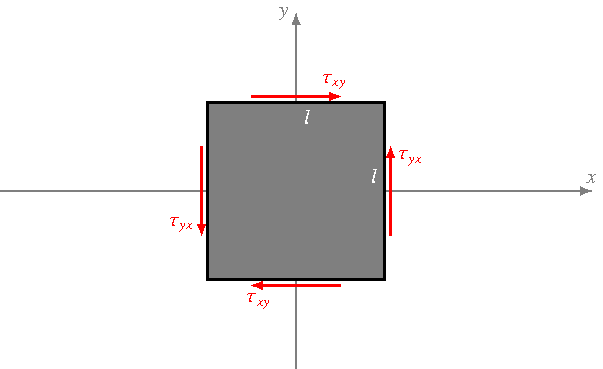
\includegraphics{chapters/2/drehmoment.pdf}
\caption{Drehmoment um die $z$-Achse der Schwerkräfte auf einen Würfel
mit Kantenlänge $2l$. Gezeigt sind nur die Komponenten von $\bm{\tau}$,
die zu einem Drehmoment führen.
\label{skript:drehmoment}}
\end{figure}
In diesem Abschnitt wollen wir nachweisen, dass der Spannungstensor
symmetrisch ist.
Dazu betrachten wir das Drehmoment, welches die Scherkräfte auf einen
kleinen Würfel mit Kantenlänge $2l$ ausüben (Abbildung \ref{skript:drehmoment}).

Der Würfel hat die Masse $m=\varrho(2l)^3$.
Das Trägheitsmoment eines Würfels mit Masse $m$ und Kantenlänge $2l$
ist
\[
I_z
=
\frac1{12}m((2l)^2+(2l)^2)
=
\frac1{12}\varrho 8l^3\cdot8l^2
=
\frac{16}{3}\varrho l^5.
\]
Der Drehimpuls um die $z$-Achse ist $L_z=I_z\omega$.

Aus Abbildung~\ref{skript:drehmoment} kann man die Scherkräfte auf den
Seitenflächen ablesen, sie sind $\tau_{xy}4l^2$ bzw.~$\tau_{yx}4l^2$,
ihr Hebelarm ist $l$.
Das resultierende Drehmoment um die $z$-Achse ist daher
\[
M_z = 8l^3\tau_{xy} - 8l^3\tau_{yx}.
\]
Die Bewegungsgleichungen eines starren Körpers besagen jetzt, dass
für die Winkelgeschwindigkeit der Drehung des Würfels um die $z$-Achse
die Gleichung
\[
\frac{dL_z}{dt}
=
M_z
\qquad\Rightarrow\qquad
I_z\dot\omega
=
M_z
\qquad\Rightarrow\qquad
\dot\omega
=
\frac{M_z}{I_z}
=
\frac{8l^3(\tau_{xy}-\tau_{yx})}{\frac{16}{3}l^5}
=
\frac{3}{2l^2}(\tau_{xy}-\tau_{yx}).
\]
Wir nehmen an, es sei $\tau_{xy}\ne\tau_{yx}$.
Lässt man $l$ gegen $0$ gehen, folgt die Aussage, dass die
Winkelgeschwindigkeit eines sehr kleinen Würfels im Fluid sich mit beliebig
schnell anwachsender Winkelgeschwindigkeit drehen müsste.
Dieses unphysikalische Resultat erlaubt zu schliessen, dass
$\tau_{xy}=\tau_{yx}$ sein muss und dass nur ein
symmetrischer Spannungstensor ein physikalisches Fluid beschreibt.

\subsubsection{Druck und Spannungen}
Die Diagonalelemente des Spannungstensors $\bm{\tau}$ beschreiben
Normalkräfte auf ein Volumenelement des Fluids.
Im Gleichgewicht sind sie alle gleich gross und stimmen mit dem
negativen {\em (hydrostatischen) Druck} überein, wir setzen daher
\index{Druck}
\index{hydrostatischer Druck}
\[
p=-\frac13\operatorname{Spur}\bm{\tau}.
\]
Wir können daher $\bm{\tau}$ zerlegen in eine Diagonalmatrix
mit Elementen $-p$ auf der Diagonalen und eine spurlose Matrix
\[
\bm{\tau} = -pE + \bm{\sigma},
\]
$E$ ist die Einheitsmatrix.
Die spurlose symmetrische Matrix $\bm{\sigma}$ heisst auch
{\em Spannungsdeviator}.
\index{Spannungsdeviator}

Für die Bewegungsgleichung brauchen wir die Divergenz beider Terme.
Die Druckterme sind alle gleich, nach
Definition~\ref{skript:definition divergenz} ist
\[
(\nabla\cdot(pE))_x
=
\sum_i
\frac{\partial p\delta_{xi}}{\partial i}
=
\frac{\partial p}{\partial x}
\qquad\Rightarrow\qquad
\nabla\cdot(pE)
=
\nabla p.
\]
Damit wird die Bewegungsgleichung 
\begin{equation}
\frac{\partial \varrho\vec{v}}{\partial t}
=
-\nabla\cdot(\varrho\vec{v}\vec{v})
+\varrho\vec b
-\nabla p
+\nabla\cdot\bm{\sigma}
\label{skript:navier-stokes2}
\end{equation}
Die Scherkräfte sind in einem newtonschen Fluid proportional zu
den Schergeschwindigkeiten.
Man kann zeigen (siehe \cite[p.~172]{skript:kaperengler}), dass $\bm{\sigma}$
geschrieben werden kann als
\[
\bm{\sigma}
=
2\nu\biggl(\bm{\varepsilon} - \frac13(\nabla\cdot\vec{v})E\biggr)
\qquad\text{mit}\qquad
\bm{\varepsilon}=\frac12\bigl(\nabla\vec{v}+(\nabla\vec{v})^t\bigr).
\]
Die spezielle Form von $\bm{\varepsilon}$ ist notwendig, damit die Matrix
$\bm{\varepsilon}$ symmetrisch wird.
Der zweite Term im Ausdruck von $\bm{\sigma}$ ist nötig, damit die Spur
\[
\operatorname{Spur}{\bm{\sigma}}
=
2\nu(\operatorname{\varepsilon} - \nabla\cdot\vec{v})
=
2\nu
\frac12
\biggl(
\sum_i \frac{\partial v_i}{\partial i}
+
\frac12
\sum_i \frac{\partial v_i}{\partial i}
-
\nabla\cdot\vec{v}
\biggr)
=
0
\]
von $\bm{\sigma}$ verschwindet.

Die Divergenz $\nabla\cdot\bm{\sigma}$ von $\bm{\sigma}$ kann damit explizit
durch die Geschwindigkeit ausgedrückt werden.
Wir berechnen die Divergenz der einzelnen Terme:
\begin{align}
(\nabla\cdot\bm{\varepsilon})_x
&=
\sum_i\frac{\partial \varepsilon_{ix}}{\partial i}
=
\frac12
\sum_i\frac{\partial}{\partial i}\biggl(
\frac{\partial v_i}{\partial x}+\frac{\partial v_x}{\partial i}
\biggr)
=
\frac{\partial}{\partial x}
\sum_i\frac{\partial v_i}{\partial i}
+
\frac12
\sum_i \frac{\partial^2 v_x}{\partial i^2}
=
\frac12\frac{\partial}{\partial x}
(\nabla\cdot\vec{v})
+
\frac12\Delta v_x
\notag
\\
\nabla\cdot\bm{\varepsilon}
&=
\frac12\nabla(\nabla\cdot\vec{v})
+
\frac12\Delta\vec{v}
\notag
\\
(\nabla\cdot(\nabla\cdot\vec{v})E)_x
&=
\sum_i \frac{\partial}{\partial i} (\nabla\cdot\vec{v}E)_{xi}
=
\sum_i \frac{\partial}{\partial i} (\nabla\cdot\vec{v}\delta_{xi})
=
\frac{\partial}{\partial x}(\nabla\cdot\vec{v})
\notag
\\
\nabla\cdot(\nabla\cdot\vec{v})E)
&=
\nabla(\nabla\cdot\vec v)
\notag
\\
\intertext{und erhalten so für die Divergenz von $\bm{\sigma}$:}
\nabla\cdot\bm{\sigma}
&=
2\nu\biggl(
\nabla\cdot\bm{\varepsilon}
-\frac13\nabla\cdot((\nabla\cdot\vec{v})E)
\biggr)
=
2\nu\biggl(
\frac12
\nabla(\nabla\cdot\vec{v})
+
\frac12\Delta\vec{v}
-\frac13
\nabla(\nabla\cdot\vec{v})
\biggr)
\\
&=
\nu\Delta\vec{v}
+\frac{\nu}3\nabla(\nabla\cdot\vec{v}).
\label{skript:sigmadiv}
\end{align}

\subsubsection{Inkompressible Strömung}
In einem inkompressiblen Fluid ist $\nabla\cdot\vec{v}=0$, dann fällt
der zweite Term in \eqref{skript:sigmadiv} weg.
Die Strömungsgleichung eines inkompressiblen Fluids erhält damit die
einfache Form
\begin{equation}
\frac{\partial\vec{v}}{\partial t}
=
-\nabla\cdot(\vec{v}\vec{v})
+\vec{b}
-\frac1{\varrho}(\nabla p
-\nu\Delta\vec{v}),
\label{skript:inkompressibel newtonsch}
\end{equation}
die klassische Navier-Stokes Gleichung.

\subsection{Zustandsgleichungen}
Die Dichte hängt vor allem auch von der Temperatur ab.
In den Ozeanen ändert die Dichte des Wassers mit dem Salzgehalt.
Eine vollständige Beschreibung der Strömung in Ozeanen oder der
Atmosphäre muss daher auch noch weitere Variablen modellieren.
In Kapitel~\ref{chapter:wetter und klima} haben wir bereits auf die
Wärmeleitungsgleichungen hingewiesen.

Die Felder $T$, $p$ und $\varrho$ sind bei einem idealen Gas miteinander
durch die Zustandsgleichung
\[
p=\varrho T R_s
\]
mit der spezifischen Gaskonstante $R_s$ verbunden.
Für den Zusammenhang von Dichte, Temperatur und Salzgehalt gibt
es jedoch kein derart einfaches Modell.
Eine weitere Kopplung zwischen der Temperatur und der
Strömung entsteht durch die Viskosität $\nu$, die sehr stark
von der Temperatur abhängt.
Auch dafür gibt es keine einfachen Modell.

In vielen Fällen schwanken die physikalischen Grössen nur geringfügig
um einen Mittelwert.
Zum Beispiel hängt die Dichte $\varrho$ von Meerwasser sowohl von
der Temperatur $T$ als auch vom Salzgehalt $h$ ab, die Dichte ist
also eine Funktion $\varrho(T,h)$.
Wir können $\varrho$ als Taylorreihe um die mittlere Temperatur $T_0$
und den mittleren Salzgehalt $h_0$ entwickeln:
\[
\varrho(T,h)
=
\varrho_0 -\alpha(T-T_0) + \beta(h-h_0).
\]
In Klimamodellen betrachten wir typischerweise nur kleine Abweichungen
von Mittelwerten, so dass ein solches Modell sehr erfolgreich sein kann.

\subsection{Boussinesq-Approximation}
Die Strömung in der Erdatmosphäre kann offensichtlich nicht als
inkompressibel betrachtet werden, die Dichte ist offenbar nicht
konstant.
Der Zustand der Atmosphäre weicht jedoch nur wenig einem mittleren
Dichteprofil $\varrho_0$ ab, welches im wesentlich durch das Temperaturprofil
festgelegt ist.
Im Normalzustand nimmt die Temperatur der Atmosphäre ziemlich genau
linear ab bis zur Höhe der Thermopause.
Auf die horizontale Komponente der Strömung hat eine Abweichung des
Temperaturprofils kaum einen Einfluss, denn andere Terme der
Navier-Stokes-Gleichung
\eqref{skript:navier-stokes2}
sind bedeutender.
Für die vertikale Bewegung ist der Term der äusseren Kräfte,
nämlich die Schwerkraft, dominant.
Wir können dies berücksichtigen, indem wir die Erdbeschleunigung
$g$ durch
\begin{equation}
g\frac{\varrho}{\varrho_0}
\label{skript:boussinesq}
\end{equation}
ersetzen.
Diese Approximation ist bekannt als die Boussinesq-Approximation.
Für unsere Zwecke hier brauchen wir nicht mehr als \eqref{skript:boussinesq}.
Dies wird bei der Herleitung der Lorenz-Gleichung in Abschnitt
\ref{section:lorenz-modell} benötigt.
Für die vollständigen Boussinesq-Gleichungen siehe \cite{skript:kaperengler}.

%In der Navier-Stokes-Gleichung können wir die horizontale Bewegung
%von der vertikalen vollständig trennen.
%Wir schreiben dazu
%\[
%\vec{u}
%=
%\begin{pmatrix}v_x\\v_y\end{pmatrix},
%\qquad
%w=v_z.
%\]
%Ausser in den für den Auftrieb wesentlichen Termen (Druck und äussere Kräfte)
%betrachten wir die Dichte als konstant.
%Die Kontinuitätsgleichung wird daher zu
%\[
%\nabla\cdot\vec{u}\frac{\partial w}{\partial z} = 0.
%\]
%Dies besagt, dass die Quellen des horizontalen Strömungsfeldes 
%durch die Vertikalströmung gespeist werden.
%Die horizontale Bewegungsgleichung bleibt bis auf den Druckterm
%erhalten.

\subsection{Inkompressible zweidimensionale Strömung}
Die Kontinuitätsgleichung
und die Navier-Stokes-Gleichung gelten auch für eine zweidimensionale
Strömung.
Im Allgmeinen ist die Strömung nicht wesentlich leichter zu berechnen.
Nur im Falle einer inkompressiblen Strömung oder der Boussinesq-Approximation
spielt die Dichte in den Gleichungen keine Rolle, was erlaubt,
sie weiter zu vereinfachen:
\begin{align}
0
&=
-\nabla\cdot\vec v
\label{skript:2dim kontinuitaet}
\\
\frac{\partial \vec{v}}{\partial t}
&=
-\nabla\cdot(\vec{v}\vec{v})+\vec b + \frac1{\varrho}\nabla\cdot\bm{\tau}.
\label{skript:2dim navier-stokes}
\end{align}
Im Falle der Boussinesq-Approximation kommt auf der rechten Seite noch
ein Term für die Auftriebskraft hinzu.

Die Gleichungen
\eqref{skript:2dim kontinuitaet}
und
\eqref{skript:2dim navier-stokes}
bilden ein System von partiellen Differentialgleichungen für die zwei
unbekannten Funktionen $v_x$ und $v_y$, die Komponenten der 
Strömungsgeschwindigkeit.
Wir werden im Folgenden zeigen, dass die 
\eqref{skript:2dim kontinuitaet}
ermöglicht, das System auf eine einzelne partielle Differentialgleichung
für nur eine einzige Funktion zu reduzieren.

\subsubsection{Satz von Green}
\begin{figure}
\centering
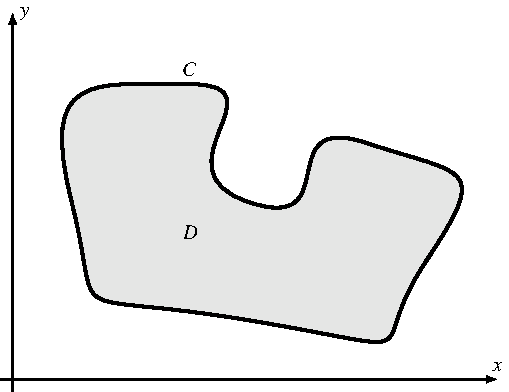
\includegraphics{chapters/2/green-curve.pdf}
\caption{Satz von Green: Das Wegintegral entlang der Randkurve $C$
stimmt mit dem zweifachen Integral über $D$ überein.
\label{skript:green-kurve}}
\end{figure}
Die Kontinuitätsgleichung 
\eqref{skript:2dim kontinuitaet}
ist ausgeschrieben
\[
0
=
\nabla\cdot\vec v
=
\frac{\partial v_x}{\partial x} + \frac{\partial v_y}{\partial y}.
\]
Die Divergenz auf der rechten Seite kommt auch im Satz von Green
vor:

\begin{satz}[Green]
\label{skript:2dim green}
Sei $D$ in kompaktes Gebiet in der $x$-$y$-Ebene mit Rand $\partial D=C$.
Weiter seien $f,g\colon D\to\mathbb R$ stetige Funktionen, die in $D$ 
stetig differenzierbar sind.
Dann gilt
\begin{equation}
\iint_{D}
\frac{\partial g(x,y)}{\partial x}
-
\frac{\partial f(x,y)}{\partial y}\,dx\,dy
=
\oint_C (f(x,y)\,dx + g(x,y)\,dy)
\label{skript:green formel}
\end{equation}
(Abbildung~\ref{skript:green-kurve}).
\end{satz}

Das Integral auf der rechten Seite wird mit Hilfe einer Parametrisierung
$\gamma\colon [a,b]\to\mathbb R^2$ der Randkurve $C$ definiert.
\begin{align*}
\oint_C f(x,y)\,dx
&=
\int_a^b f(\gamma_x(t),\gamma_y(t))\dot{\gamma}_x(t)\,dt,
\\
\oint_C g(x,y)\,dy
&=
\int_a^b g(\gamma_x(t),\gamma_y(t))\dot{\gamma}_y(t)\,dt.
\end{align*}
Es kann auch vektoriell mit dem Skalarprodukt als
\[
\oint_C
\underbrace{
\begin{pmatrix}f\\g\end{pmatrix}
}_{\displaystyle =\vec{w}}
\cdot
\begin{pmatrix}\dot\gamma_x\\\dot\gamma_y\end{pmatrix}
\,dt
=
\oint_C \vec{w}\cdot\dot\gamma(t)\,dt
=:
\oint_C \vec{w}\cdot d\vec{s}
\]
geschrieben werden kann.

\subsubsection{Stromfunktion}
Wir wenden den Satz \ref{skript:2dim green} von Green auf die
Funktionen $f(x,y)=-v_y(x,y)$ und $g(x,y)=v_x(x,y)$ an.
Die Formel \eqref{skript:green formel} ergibt
\begin{equation}
\oint_C (-v_y(x,y)\,dx + v_x(x,y)\,dy)
=
\iint_D
\underbrace{
\frac{\partial v_x(x,y)}{\partial x}
+
\frac{\partial v_y(x,y)}{\partial y}
}_{\displaystyle=0}
\,dx\,dy
=
0.
\label{skript:wegunabh}
\end{equation}
Man kann dieses Resultat auch wie folgt interpretieren.
Wenn $C_1$ und $C_2$ zwei Kurven sind, die den Punkt $A$ mit dem Punkt $B$
verbinden, dann lässt sich eine geschlossene Kurve $C$ konstruieren, indem
zuerst die Kurve $C_1$ von $A$ nach $B$ durchlaufen wird und dann die
Kurve $C_2$ in umgekehrter Richtung von $B$ nach $A$.
Die Formel \eqref{skript:wegunabh} besagt dann, dass 
\begin{align*}
0
&=
\oint_{C} (-v_y(x,y)\,dx + v_x(x,y)\,dy)
\\
&=
\int_{C_1} (-v_y(x,y)\,dx + v_x(x,y)\,dy)
-
\int_{C_2} (-v_y(x,y)\,dx + v_x(x,y)\,dy)
\end{align*}
oder
\begin{align*}
\Rightarrow
\qquad
\int_{C_1} (-v_y(x,y)\,dx + v_x(x,y)\,dy)
&=
\int_{C_2} (-v_y(x,y)\,dx + v_x(x,y)\,dy).
\end{align*}
Das Wegintegral hängt also nicht von der Wahl des Weges ab, jeder Weg
von $A$ nach $B$ führt auf den gleichen Wert des Integrals.

\begin{figure}
\centering
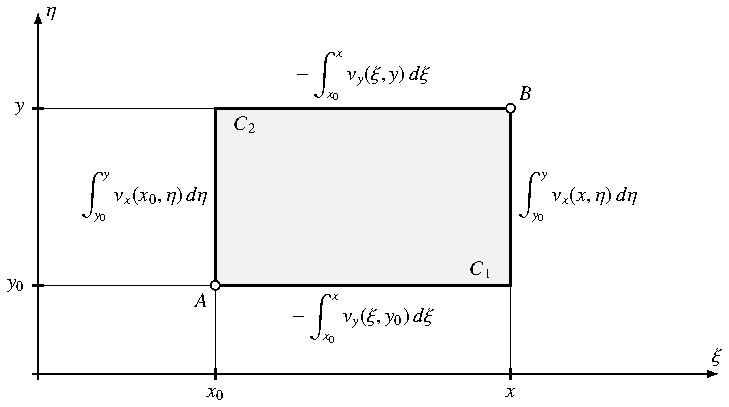
\includegraphics{chapters/2/green-curves.pdf}
\caption{Verschiedene Pfade zur Berechnung der Funktion $\psi(B)$
führen auf den gleichen Wert von $\psi(B)$ und ermöglichen, die partiellen
Ableitungen zu berechnent.
\label{skript:psi-pfade}}
\end{figure}

Wir halten den Punkt $A$ fest und definieren die Funktion
\[
\psi(B)
=
\int_C (-v_y(x,y)\,dx + v_x(x,y)\,dy)
\]
für einen beliebigen Weg von $A$ nach $B$. 
Zum Beispiel können für die Berechnung die Kurven
$C_1$ oder $C_2$ in Abbildung~\ref{skript:psi-pfade}
verwendet werden.
Damit lassen sich die Integrale ausschreiben:
\begin{align*}
\psi(x,y)
&=
\int_{C_1} (-v_y(x,y)\,dx + v_x(x,y)\,dy)
=
-\int_{x_0}^x v_y(\xi, y_0)\,d\xi
+
\int_{y_0}^y v_x(x,\eta)\,d\eta
\\
&=
\int_{C_2} (-v_y(x,y)\,dx + v_x(x,y)\,dy)
=
\int_{y_0}^y v_x(x_0,\eta)\,d\eta
-
\int_{x_0}^x v_y(\xi,y)\,d\xi.
\end{align*}
Diese Ausdrücke erlauben uns, die partiellen Ableitungen von $\psi(x,y)$
zu berechnen.
Für die Ableitung nach $x$ verwenden wir den zweiten Ausdruck, für die
Ableitung nach $y$ den ersten.
Wir erhalten
\begin{align*}
\frac{\partial\psi(x,y)}{\partial x}
&=
-\frac{\partial}{\partial x} \int_{x_0}^x v_y(\xi,y)\,d\xi
=
-v_y(x,y),
\\
\frac{\partial\psi(x,y)}{\partial y}
&=
\frac{\partial}{\partial y} \int_{y_0}^y v_x(x,\eta)\,d\eta
=
v_x(x,y).
\end{align*}
In vektorieller Form kann man dies auch als
\begin{equation}
\vec{v}
=
\begin{pmatrix}v_x\\v_y \end{pmatrix}
=
\underbrace{
\begin{pmatrix}0&-1\\1&0\end{pmatrix}
}_{\displaystyle=J}
\begin{pmatrix}
\frac{\partial\psi}{\partial x}\\
\frac{\partial\psi}{\partial y}
\end{pmatrix}
=
J\nabla\psi
\label{skript:Jnablapsi}
\end{equation}
schreiben.
Aus der Funktion $\psi$ lässt sich das Vektorfeld $\vec{v}$ also wieder
rekonstruieren.
Sie heisst die {\em Stromfunktion} des Vektorfeldes $\vec{v}$.
\index{Stromfunktion}
Natürlich ist $\psi(x,y)$ nur bis auf eine Konstante bestimmt.

Umgekehrt ist für jede beliebige Funktion $\varphi(x,y)$ das Vektorfeld
$\vec{u}=J\nabla\varphi$ divergenzfrei:
\begin{align*}
\nabla\cdot\vec{u}
=
\frac{\partial}{\partial x}
\biggl(-\frac{\partial\varphi}{\partial y}\biggr)
+
\frac{\partial}{\partial y}
\biggl(\frac{\partial\varphi}{\partial x}\biggr)
=
-\frac{\partial^2\varphi}{\partial x\,\partial y}
+\frac{\partial^2\varphi}{\partial y\,\partial x}
=
0.
\end{align*}
Die Darstellung \eqref{skript:Jnablapsi} des Geschwindigkeitsfeldes 
erlaubt eine geometrische Interpretation.
Der Gradient $\nabla\psi$ ist ein Vektorfeld, welches auf den
Niveaulinien der Funktion $\psi$ senkrecht steht.
Je schneller die Zunahme von $\psi$, desto grösser ist der
Vektor $\nabla\psi$.

Die Matrix $J$ ist eine Drehmatrix, sie dreht Vektoren um $90^\circ$ 
im Gegenuhrzeigersinn.
Die Vektoren $J\nabla\psi$ sind also tangential an die Niveaulinien,
die Niveaulinien sind also gleichzeitig die Stromlinien der Strömung.
Ist die Strömung auf ein kompaktes Gebiet beschränkt, dann ist der
Rand des Gebietes eine Stromlinie, also eine Niveaulinie von $\psi$.
Da $\psi$ nur bis auf eine Konstante festgelegt ist, kann man $\psi$
so wählen, dass der Rand des Gebietes durch die Gleichung $\psi(x,y)=0$
beschrieben wird.

\index{Stromlinien}
\begin{figure}
\centering
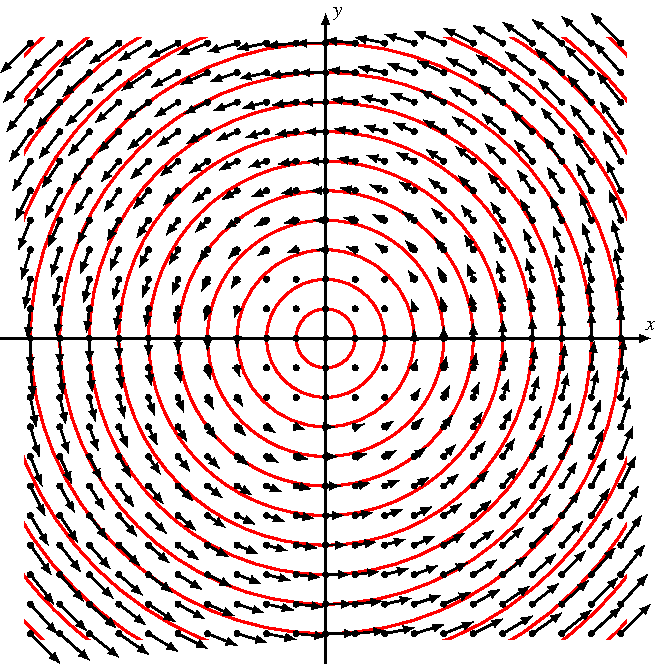
\includegraphics{chapters/2/rotation.pdf}
\caption{Strömungsfunktion $\psi(x,y)=a(x^2+y^2)$ und das zugehörige
Vektorfeld.
Die Strömungsgeschwindigkeit ist proportional zum Radius, es handelt
sich also um eine starre Drehung um den Nullpunkt.
\label{skript:rotation}}
\end{figure}
Die Funktion $\psi(x,y)=a(x^2+y^2)$ führt auf das Vektorfeld
\[
\vec{v}
=
J\nabla\psi
=
2a
\begin{pmatrix}
-y\\x
\end{pmatrix}
\]
(Abbildung~\ref{skript:rotation}).
Die Strömungsgeschwindigkeit ist $2a\sqrt{x^2+y^2}=2ar$, es handelt sich
also um eine starre Drehung um den Nullpunkt des Koordinatensystems mit
Winkelgeschwindigkeit $\omega=2a$.

\subsubsection{Vorticity}
Wir suchen eine Grösse, mit der wir das Ausmass messen können, wie schnell
sich das Fluid dreht.
Die Winkelgeschwindigkeit bei der Drehung um den Punkt $(x,y)$ können wir
durch Vergleich der Geschwindigkeit an den Punkten $(x\pm h,y)$ und
$(x,y\pm h)$ finden.
Es ist
\[
\omega
=
\frac{v_y(x+h),y) - v_y(x-h,y)}{2h}
=
\frac{-v_x(x,y+h) + v_x(x,y-h)}{2h}.
\]
Beim Grenzübergang $h\to 0$ erhalten wir
\[
\omega
=
\frac{\partial v_y(x,y)}{\partial x}
=
-\frac{\partial v_x{x,y}}{\partial y}
\qquad\text{oder}\qquad
2\omega
=
\frac{\partial v_y}{\partial x}-\frac{\partial v_x}{\partial y}.
\]
Damit haben wir eine Grösse gefunden, die als Mass für die Drehgeschwindigkeit
dienen kann.
\index{Vorticity}
\begin{definition}
Ist $\vec{v}$ das Geschwindigkeitsfeld der Strömung, dann schreiben wir
\[
\nabla\times\vec{v}
=
\frac{\partial v_y}{\partial x}-\frac{\partial v_x}{\partial y}
=
\zeta.
\]
Die Funktion $\zeta$ heisst die {\em Vorticity} des Strömungsfeldes.
\end{definition}

Beschreibt man die Strömung mit Hilfe der Strömungsfunktion, dann gilt
für die Vorticity
\begin{equation}
\zeta
=
\nabla\times\vec{v}
=
\nabla\times J\nabla\psi
=
\frac{\partial}{\partial x}
\biggl(-\frac{\partial\psi}{\partial y}\biggr)
-
\frac{\partial}{\partial x}
\frac{\partial\psi}{\partial x}
=
-\biggl(
\frac{\partial^2\psi}{\partial x^2}
+
\frac{\partial^2\psi}{\partial y^2}
\biggr)
=
-\Delta \psi.
\label{skript:stroemung-vorticity}
\end{equation}
Der Laplace-Operator verbindet also die Strömungsfunktion direkt mit der
Vorticity.
Für die Strömung in einem kompakten Gebiet $\Omega$ ist der Rand eine
Niveaulinie von $\psi$.
Wie früher dargelegt können wir $\psi$ so wählen, dass $\psi=0$ gilt auf
dem Rand.
Bei gegebener Vorticity $\zeta$ ist daher $\psi$ die Lösung der
partiellen Differentialgleichung
\begin{equation}
\Delta \psi = -\zeta\quad\text{in $\Omega$}
\qquad
\psi = 0\quad\text{auf $\partial\Omega$}.
\label{skript:zetapsielliptisch}
\end{equation}
Die Theorie der elliptischen partiellen Differentialgleichungen 
sagt, dass $\psi$ eindeutig bestimmt ist.
Statt die Strömungsgleichungen für $\psi$ zu lösen, können wir
also auch versuchen, eine Gleichung für die Vorticity $\zeta$
aufzustellen und dann mit Hilfe des elliptischen partiellen
Randwertproblems \eqref{skript:zetapsielliptisch} die Strömungsfunktion
und schliesslich $\vec{v}$ bestimmen.

Um die Differentialgleichung für $\zeta$ zu finden, wenden wir den
Operator $\nabla\times\mathstrut$ auf die Bewegungsgleichung
\eqref{skript:2dim navier-stokes}
an:
\[
\nabla\times\frac{\partial \vec{v}}{\partial t}
=
-\nabla\times(\nabla\cdot(\vec{v}\vec{v}))+\nabla\times\vec b + \nabla\times\biggl(\frac1{\varrho}\nabla\cdot\bm{\tau}\biggr).
\]
Die linke Seite ist die Zeitableitung der Vorticity.
Die Divergenz von $\vec{v}\vec{v}$ ist 
\[
(\nabla\cdot(\vec{v}\vec{v}))_j
=
\sum_i \frac{\partial}{\partial i}v_iv_j
=
\biggl(\sum_i \frac{\partial v_i}{\partial i}\biggr)v_j
+
\sum_i v_i\frac{\partial v_j}{\partial i}
=
(\underbrace{\nabla\cdot\vec{v}}_{\displaystyle=0})v_j
+
\vec{v}\cdot\nabla v_j.
\]
Es folgt
\[
\nabla\cdot(\vec{v}\vec{v})
=
\vec{v}\cdot\nabla \vec{v}.
\]
Daraus kann man jetzt auch die Vorticity berechnen:
\begin{align*}
\nabla\times(\nabla\cdot(\vec{v}\vec{v}))
&=
\nabla\times(\vec{v}\cdot\nabla\vec{v})
=
\frac{\partial}{\partial x}(\vec{v}\cdot\nabla v_y)
-
\frac{\partial}{\partial y}(\vec{v}\cdot\nabla v_x)
\\
&=
\vec{v}\cdot\nabla
\biggl(\frac{\partial v_y}{\partial x}-\frac{\partial v_x}{\partial y}\biggr)
+
\frac{\partial\vec{v}}{\partial x} \cdot\nabla v_y
-
\frac{\partial\vec{v}}{\partial y} \cdot\nabla v_x
\\
&=
\vec{v}\cdot\nabla\zeta
+
\frac{\partial v_x}{\partial x} \frac{\partial v_y}{\partial x}
+
\frac{\partial v_y}{\partial x} \frac{\partial v_y}{\partial y}
-
\frac{\partial v_x}{\partial y} \frac{\partial v_x}{\partial x}
-
\frac{\partial v_y}{\partial y} \frac{\partial v_x}{\partial y}
\\
&=
\vec{v}\cdot\nabla\zeta
+
\frac{\partial v_x}{\partial x}
\biggl(\frac{\partial v_y}{\partial x}-\frac{\partial v_x}{\partial y}\biggr)
+
\frac{\partial v_y}{\partial y}
\biggl(\frac{\partial v_y}{\partial x}-\frac{\partial v_x}{\partial y}\biggr)
\\
&=
\vec{v}\cdot\nabla\zeta
+
(\nabla\cdot\vec{v})\zeta
=
\vec{v}\cdot\nabla\zeta.
\end{align*}
Wir waren also nicht ganz erfolgreich, die Geschwindigkeit aus der
Bewegungsgleichung zu eliminieren.
Wir haben nur die Form
\[
\frac{\partial \zeta}{\partial t}
=
-\vec{v}\cdot\nabla\zeta
+\nabla\times\vec b
+ \nabla\times\biggl(\frac1{\varrho}\nabla\cdot\bm{\tau}\biggr)
\]
erreicht.
Ausserdem ist es möglich, dass die Spannungen $\bm{\tau}$ ebenfalls von
den Geschwindigkeiten abhängig sind.

Wir können aber die Vorticity auch noch durch die Strömungsfunktion
ausdrücken.
Ersetzen wir $\zeta=-\Delta\psi$ in der Bewegungsgleichung, erhalten
wir
\begin{equation}
\frac{\partial \Delta \psi}{\partial t}
=
-J\nabla\psi\cdot\nabla\Delta\psi
+\nabla\times\vec b
+ \nabla\times\biggl(\frac1{\varrho}\nabla\cdot\bm{\tau}\biggr).
\label{skript:voritictyequation}
\end{equation}
Jetzt ist die Strömung vollständig durch die einzige unbekannte Funktion 
$\psi$.

Der erste Term auf der rechten Seite von \eqref{skript:voritictyequation}
kann noch etwas kompakter geschrieben werden.
Es ist
\begin{align*}
(J\nabla f)\cdot(\nabla g)
&=
\begin{pmatrix}
-\frac{\partial f}{\partial y}
\\
\frac{\partial f}{\partial x}
\end{pmatrix}
\cdot
\begin{pmatrix}
\frac{\partial g}{\partial x}\\
\frac{\partial g}{\partial y}
\end{pmatrix}
=
\frac{\partial f}{\partial x}
\frac{\partial g}{\partial y}
-\frac{\partial f}{\partial y}
\frac{\partial g}{\partial x}.
\end{align*}
Der Ausdruck auf der rechten Seite kommt auch in anderem Zusammenhang vor.

\begin{definition}
Seien $f$ und $g$ Funktionen der Variablen $x$ und $y$.
Dann heisst
\[
\frac{\partial(f,g)}{\partial(x,y)}
=
\frac{\partial f}{\partial x}
\frac{\partial g}{\partial y}
-
\frac{\partial f}{\partial y}
\frac{\partial g}{\partial x}
\]
die
{\em Funktionaldeterminante} oder {\em Jacobische Determinante} von
$f$ und $g$.
\end{definition}
\index{Funktionaldeterminante}
\index{Jacobi-Determinante}
Mit dieser Definition wird die Bewegungsgleichung
\begin{equation}
\frac{\partial \Delta \psi}{\partial t}
=
\nabla\times\vec b
+ \nabla\times\biggl(\frac1{\varrho}\nabla\cdot\bm{\tau}\biggr)
-\frac{\partial(\psi,\Delta\psi)}{\partial(x,y)}.
\label{skript:psidgl}
\end{equation}
Im Falle der Boussinesq-Näherung kommt noch ein Term für den
Auftrieb hinzu.

\subsubsection{Spannungen und Stromfunktion}
Für eine newtonsche Flüssigkeit haben wir in 
\eqref{skript:inkompressibel newtonsch}
bereits den Spannungstensor durch den Druck und die Spannungen
ausgedrückt.
Aus der Bewegungsgleichung für die Geschwindigkeit haben wir die
Differentialgleichung \eqref{skript:psidgl} erhalten, indem
wir den Operator $\nabla\times\mathstrut$ angewendet haben.
Wir müssen jetzt also 
\[
\nabla\times\biggl(\frac1{\varrho}(\nabla p-\nu\Delta\vec{v})\biggr)
=
\frac{1}{\varrho}
\biggl(
\nabla\times\nabla p
-
\nu \nabla\times\Delta\vec{v}
\biggr)
=
\frac1{\varrho}
\biggl(
\frac{\partial}{\partial x}\frac{\partial p}{\partial y}
-
\frac{\partial}{\partial y}\frac{\partial p}{\partial x}
-\nu\Delta\nabla\times\vec{v}
\biggr)
\]
berechnen.
Der erste Term fällt weg, weil es auf die Reihenfolge der zweiten
Ableitungen nicht ankommt.
Im zweiten Term haben wir angenommen, dass $\nu$ nicht vom Ort
abhängig.
Dies ist genau genommen nicht richtig, da $\nu$ zum Beispiel
stark von der Temperatur abhängt, die ebenfalls nicht konstant sein
muss.
Der zweite Term in der Klammer ist natürlich einfach
$\nu\Delta\zeta=-\nu\Delta^2\psi$.
Damit bekommen wir die Bewegungsgleichung für $\psi$ in der Form
\begin{equation}
\frac{\partial \Delta \psi}{\partial t}
=
\nabla\times\vec b
+\frac{\nu}{\varrho}\Delta^2\psi
-\frac{\partial(\psi,\Delta\psi)}{\partial(x,y)}.
\label{skript:psidgl2}
\end{equation}



%
% lorenz.tex -- Lorenz-Modell
%
% - Herleitung aus den Gleichungen der Fluiddynamik
% - Dynamik aus numerischen Simulationen
%
% (c) 2018 Prof Dr Andreas Müller, Hochschule Rapperswil
%
\section{Lorenz-Modell\label{section:lorenz-modell}}
Sowohl die Atmosphäre als auch die Ozeane werden durch die hydrodynamischen
Gleichungen beschrieben.
Es stellt sich damit die Frage, in welchem Masse sich daraus eine praktikable
Vorhersage sowohl von Wetter also auch des Klimas ableiten lässt.
In den Sechzigerjahren hat Edward Lorenz versucht, diese Frage mit einem
vereinfachten Modell zu beantworten.
Ziel dieses Abschnittes ist, das Lorenz-Modell aus den Gleichungen der
Fluiddynamik herzuleiten.

\subsection{Modellbeschreibung}
\begin{figure}
\centering
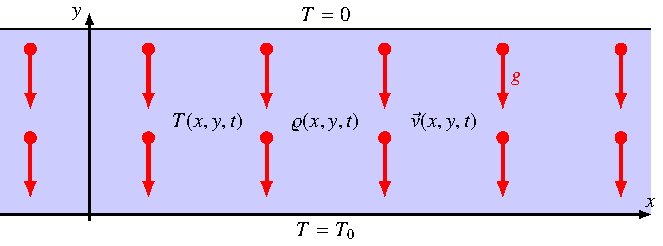
\includegraphics{chapters/2/lorenz-definition.pdf}
\caption{Definitionsgebiet für das Lorenz-Modell der Atmosphäre.
Gesucht sind Temperatur $T(x,y,t)$, Dichte $\varrho(x,y,t)$ und
Geschwindigkeit $\vec{v}(x,y,t)$ in einem Rechteckgebiet
$\mathbb R\times [0,\pi]$.
Die Temperatur ist an den Rändern vorgegeben, es gilt
$T(x,0,t)=T_0$ und $T(x,\pi,t)=0$.
Im Inneren Gebiet wird die Schwerkraft $g$ auf die Luft.
\label{skript:lorenzmodell definitionsgebiet}}
\end{figure}
Es soll ein dünner Schnitt durch die Atmosphäre modelliert werden.
Da Atmosphäre im Vergleich zur Krümmung der Erdoberfläche sehr dünn ist,
können wir sie als eben annehmen.
Wir verwenden die Koordinate $x$ parallel zur Erdoberfläche und $y$ als Höhe
(Abbildung~\ref{skript:lorenzmodell definitionsgebiet}).
Gesucht ist also die Temperatur $T(x,y,t)$ und die Dichte $\varrho(x,y,t)$
in Abhängigkeit von Position und Zeit sowie der Geschwindigkeitsvektor
\[
\vec v
=
\begin{pmatrix}v_x\\v_y\end{pmatrix}
=
\begin{pmatrix}v_x(x,y,t)\\v_y(x,y,t)\end{pmatrix}.
\]
Die Funktionen $T$, $\varrho$, $v_x$ und $v_y$ sind definiert in einem
Streifen.
Der Einfachheit halber wählen wir die Höhe des Streifens als $\pi$.
Wir können dies erreichen, indem wir die Längeneinheit geeignet wählen:
ist $h$ die ``Dicke'' der Atmosphäre\footnote{Die Konvektion in der Atmosphäre,
welche vom Lorenz-Modell vor allem beschrieben wird, findet im Wesentlichen
nur im untersten Teil der Atmosphäre, der sogenannten Troposphäre statt.
Die Troposphäre zeichnet sich aus durch mehr oder weniger lineare
Temperaturabnahme bis zur Höhe der sogenannten Tropopause in etwa
10km Höhe.
Wir können also die Höhe der Tropopause als $h$ verwenden.}, wählen wir
$h/\pi$ als Längeneinheit.
Das Definitionsgebiet für die Funktionen ist daher $R=\mathbb R\times [0,\pi]$.

Die Temperatur der Atmosphäre an der Erdoberfläche wird im wesentlichen von
der Temperatur des Bodens bestimmt, der von der einfallenden Strahlung
ergewärmt wird, es soll also $T(x,0,t)=T_0$ gelten.
Am oberen Rand des Schnittes schliesst die sehr dünne Hochatmosphäre an,
die im Wesentlichen in einem Strahlungsgleichgewicht mit der Umgebung steht.
Da wir die Dichte im wesentlichen als konstant ansehen wollen und damit
den Einfluss der Temperatur auf die Dichte nicht exakt modellieren wollen,
sind wir nicht gezwungen, eine bestimmte Temperaturskala zu verwenden.
Wir können daher willkürlich die Temperatur am oberen Rand als
$T(x,\pi,t)=0$ festlegen.

Auf das Medium im Streifen wirkt natürlich die Erdbeschleunigung,
die wir ebenfalls als konstant annehmen dürfen, da die Dicke der 
Atmosphäre im Vergleich zum Erdradius sehr klein ist.

\subsubsection{Stabile Atmosphäre}
\begin{figure}
\centering
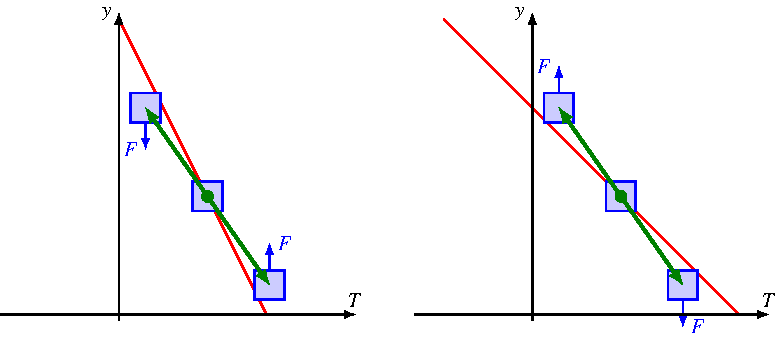
\includegraphics{chapters/2/lorenz-stabil.pdf}
\caption{Stabilität der Atmosphäre: bewegt sich ein Luftpaket in der
Atmosphäre nach oben oder unten, expandiert oder kontrahiert es und
verändert seine Temperatur adiabatisch (grün).
Ist diese Temperaturänderung grösser als der aktuelle Temperaturgradient
(links),
ändert sich die Dichte der Luft weniger stark als die der Umgebungsluft,
die Bewegung wird gestoppt, die Atmosphäre ist im Gleichgewicht.
Andernfalls wird die Bewegung beschleunigt, die Atmosphäre ist instabil
(rechts).
\label{skript:stabilitaet der atmosphaere}}
\end{figure}
Die Temperatur muss im Gebiet von unten nach oben abnehmen.
Aber auch der Druck muss mit zunehmender Höhe abnehmen. 
Wenn ein Luftpaket aufsteigt, wird es wegen des geringer werdenden
Druckes expandieren und damit adiabatisch abkühlen.
Wenn die Temperatur der umgebenden Luft schneller abnimmt als die
adiabatische Abkühlung, dann ist das Luftpaket in seiner neuen Höhe
wärmer und damit leichter als die Umgebung, es wird weiter ansteigen
(Abbildung~\ref{skript:stabilitaet der atmosphaere}).
Wenn die Temperatur der umgebenden Luft langsamer abnimmt als die
adiabatische Abkühlung, dann ist das Luftpaket in der neuen Höhe 
kälter und damit Dichter als die Umgebung, es wird wieder absinken.
Solange der Temperaturunterschied nicht zu gross ist, wird sich also ein
Zustand einstellen, in dem die Luft in Ruhe bleibt, der Wärmetransport
erfolgt ausschliesslich durch Wärmeleitung.

\subsubsection{Instabilität}
Bei genügend grosser Temperaturdifferenz wird die Atmosphäre jedoch
instabil, der Wärmetransport wird zusätzlich von Konvektion übernommen.
Die entstehenden Konvektionszellen können wegen der Translationssymmetrie
entlang der $x$-Achse an einer beliebigen Stelle entstehen, es gibt also
unendlich viele Lösungen, von denen eine gewählt werden muss.
In der Realität würden kleine Temperaturfluktionen dies unterstützen,
kleine Unterschiede in den Anfangsbedingungen führen also zu völlig
verschiedenen Strömungen.
% Abbildung?
Diese sensitive Abhängigkeit der Lösung von Anfangsbedingungen wird
oft als ein Kennzeichen von Chaos angesehen.

Im folgenden sollen zunächst die Gleichungen der Fluiddynamik auf die
vorliegende Situation spezialisiert werden.
Mit Hilfe eines geeigneten Ansatzes soll dann die partielle
Differentialgleichung weiter auf ein System von gewöhnlichen 
Differentialgleichungen reduziert werden.
In numerischen Simulationen soll schliesslich gezeigt werden, dass die 
Lorenz-Gleichungen tatsächlich chaotische Lösungen haben.

\subsubsection{Temperaturgleichung}
Wir haben in \eqref{skript:waermeleitungadvektion}
bereits eine Gleichung gefunden, welche den Wärmetransport in einem 
Fluid beschreibt.
Wir können daraus aber noch eine etwas einfacher zu handhabende Form
gewinnen, indem wir nur die Anomalie der Temperatur betrachten, also
die Abweichung vom Temperaturprofil, welches sich bei einem ruhenden
Fluid einstellt. 
Aufgrund der gewählten Geometrie ist 
\[
T_0(x,y,t)= T_0\biggl(1- \frac{y}{\pi}\biggr)
\]
in einem ruhenden Fluid, wir setzen daher
\[
\vartheta(x,y,t)
= 
T(x,y,t)
-
T_0\biggl(1-\frac{y}{\pi}\biggr)
\qquad\text{oder}\qquad
T(x,y,t)
=
T_0\biggl(1-\frac{y}{\pi}\biggr)
+
\vartheta(x,y,t)
\]
und setzen dies in die Gleichung \eqref{skript:waermeleitungadvektion}
ein.
Wir erhalten
\begin{align*}
\frac{\partial\vartheta}{\partial t}
&=
\frac{\partial T}{\partial t}
&
\Delta T
&=
\Delta \vartheta
\\
-\vec{v}\cdot\nabla T
&=
-\vec{v}\cdot\nabla\vartheta
+v_y\frac{T_0}{\pi}.
\\
\Rightarrow
\qquad
\frac{\partial\vartheta}{\partial t}
&=
-\vec{v}\cdot\nabla \vartheta
+v_y\frac{T_0}{\pi}
+
\kappa\Delta \vartheta.
\end{align*}
Die Geschwindigkeit kann mit Hilfe von $\vec{v}=-\nabla \psi$ wieder
durch die Stromfunktion ausgedrückt werden.
\begin{equation}
\frac{\partial\vartheta}{\partial t}
=
-J\nabla\psi\cdot\nabla\vartheta
+\frac{T_0}{\pi}\frac{\partial\psi}{\partial x}
+\kappa\Delta\vartheta
=
\kappa\Delta\vartheta
+\frac{T_0}{\pi}\frac{\partial\psi}{\partial x}
-\frac{\partial \psi}{\partial y}\frac{\partial \vartheta}{\partial x}
+\frac{\partial \psi}{\partial x}\frac{\partial \vartheta}{\partial y}
=
\kappa\Delta\vartheta
+\frac{T_0}{\pi}\frac{\partial\psi}{\partial x}
-
\frac{\partial(\psi,\vartheta)}{\partial(x,y)}.
\label{skript:lorenzthetagl}
\end{equation}
Man beachte, dass die Gleichung bis auf den ltzten Term linear 
in $\psi$ und $\vartheta$ ist.

\subsubsection{Bewegungsgleichung}
Die Bewegungsgleichung haben wir in
\eqref{skript:psidgl2}
bereits in die für ein zweidimensionales inkompressibles Fluid
geignete Form gebracht.
Da die Schwerkraft konstant ist, fällt der Terme $\nabla\times\vec{b}$
weg.

Aus der Boussinesq-Näherung
\eqref{skript:boussinesq}
erhalten wir noch einen Term, der den
Auftrieb beschreibt.
Auftrieb entsteht offenbar genau dann, wenn die Temperatur vom linearen
Temperaturprofil abweicht.
Wir nehmen an, dass die Dichteabweichung proportional zur Temperaturabweichung
ist, also
\[
\vec{b}
=
\begin{pmatrix}
0\\
-g(1-c\vartheta)
\end{pmatrix}
\qquad
\Rightarrow
\qquad
\nabla\times\vec{b}
=
c\frac{\partial\vartheta}{\partial x}.
\]
Damit erhalten wir die Bewegungsgleichung in der Form
\begin{equation}
\frac{\partial\Delta\psi}{\partial t}
=
\nu\Delta^2\psi 
+c\frac{\partial\vartheta}{\partial x}
-\frac{\partial(\psi,\Delta\psi)}{\partial(x,y)}.
\label{skript:lorenzpsigl}
\end{equation}
Man beachte, dass die Gleichung bis auf den letzten Term linear
in $\psi$ und $\vartheta$ ist.

\subsection{Grundgleichungen}
In den Gleichungen
\eqref{skript:lorenzthetagl}
und
\eqref{skript:lorenzpsigl}
haben wir ein partielles Differentialgleichungssystem für die beiden 
unbekannten Funktionen $\psi$ und $\vartheta$ gefunden, die wir
der besseren Übersicht halber nochmals als
\begin{equation}
\begin{aligned}
\frac{\partial\Delta\psi}{\partial t}
&=
\nu\Delta^2\psi 
+c\frac{\partial\vartheta}{\partial x}
-\frac{\partial(\psi,\Delta\psi)}{\partial(x,y)}
\\
\frac{\partial\vartheta}{\partial t}
&=
\kappa\Delta\vartheta
+\frac{T_0}{\pi}\frac{\partial\psi}{\partial x}
-
\frac{\partial(\psi,\vartheta)}{\partial(x,y)}
\end{aligned}
\label{skript:lorenzausgangsgleichung}
\end{equation}
hinschreiben.
Allerdings ist das System von dritter Ordnung, da erste Ableitungen von
$\psi$ und $\Delta\psi$ vorkommen.
Man sieht aber auch, dass keine anderen Ableitungen vorkommen als erste
Ableitungen von $\psi$ oder $\Delta\psi$.
Dies ist geeignet, die Diskussion zu vereinfachen, weshalb wird darauf
achten, diese Struktur nicht zu zerstören.
Wir können die linke Seite der Gleichungen zum Beispiel vektoriell schreiben
als
\[
\frac{\partial}{\partial t}
\begin{pmatrix}
\Delta\psi\\\vartheta
\end{pmatrix}
=
\frac{\partial}{\partial t}
\underbrace{
\begin{pmatrix}
\Delta &  0 \\
   0   &  1
\end{pmatrix}
}_{\displaystyle=D}
\underbrace{
\begin{pmatrix}
\psi\\\vartheta
\end{pmatrix}
}_{\displaystyle=u}
=
\frac{\partial}{\partial t} Du
\]
Entsprechend lassen sich die ersten zwei Terme auf der rechten Seite 
schreiben als
\[
\def\arraystretch{1.1}
\begin{pmatrix}
\nu\Delta^2     & \displaystyle c\frac{\partial}{\partial x}\\
\displaystyle \frac{T_0}{\pi}\frac{\partial}{\partial x}    &\kappa\Delta
\end{pmatrix}
\begin{pmatrix}
\psi\\\vartheta
\end{pmatrix}
=
Au.
\]
Die Operatoren $D$ und $A$ sind beide linear.

Für die Diskussion der Zeitentwicklung der Lösungen ist es nützlich,
die linearen Terme von den nichtlinearen zu trennen.
Wie bereits bemerkt treten Nichtlinearitäten nur in den
Funktionaldeterminanten auf.
Wir schreiben
\[
Nu
=
\def\arraystretch{1.9}
\begin{pmatrix}
\displaystyle
-\frac{\partial(\psi,\Delta\psi)}{\partial(x,y)}\\
\displaystyle
-\frac{\partial(\psi,\vartheta)}{\partial(x,y)}
\end{pmatrix}.
\]
Damit haben wir das Differentialgleichungssystem in der Form
\begin{equation}
\frac{\partial}{\partial t}Du
=
Au+Nu
\label{skript:allgemeinesmodell}
\end{equation}
mit den linearen Operatoren $D$ und $A$ und dem nichtlinearen Operator
$N$ schreiben.

Die allgemeine Form \eqref{skript:allgemeinesmodell} eines Klimamodells
ermöglicht uns, das Klimavorhersageproblem in dem etwas allgemeineren
Rahmen der Vorhersage für ein beliebiges nichtlineares dynamisches
System zu studieren.
Zwar ist \eqref{skript:allgemeinesmodell} immer noch ein partielles
Differentialgleichungssystem und die Operatororen $D$, $A$ und $N$
sind partielle Differentialoperatoren.
Wenn es aber gelingt, die Funktionen zu diskretisieren und durch
Vektoren in einem endlichdimensionalen Vektorraum zu ersetzen, dann
werden $D$ und $A$ zu linearen Abbildungen, die durch Matrizen beschrieben
werden können, und $N$ wird zu einer nichtlinearen Funktion auf einem
endlichdimensionalen Vektorraum.
Das Klimamodell wird also zu einer nichtlinearen gewöhnlichen
Differentialgleichung in einem endlichdimensionalen Raum.
Solche Differentialgleichungen sind im Detail studiert worden und ihre
Eigenschaften sind sehr gut verstanden.
In Kapitel~\ref{chapter:dgl} werden wir einen Teil der gut ausgebauten
Theorie zusammenfassen.
Den Weg von \eqref{skript:allgemeinesmodell} zu einer gewöhnlichen
Differentialgleichung in nur drei Dimensionen soll im folgenden 
Abschnitt~\ref{subsection:umwandlung} vorgeführt werden.

% XXX Diskussion des unendlichdimensionalen dynamischen Systems

\subsection{Umwandlung in ein gewöhnliches Differentialgleichungssystem\label{subsection:umwandlung}}
\begin{figure}
\centering
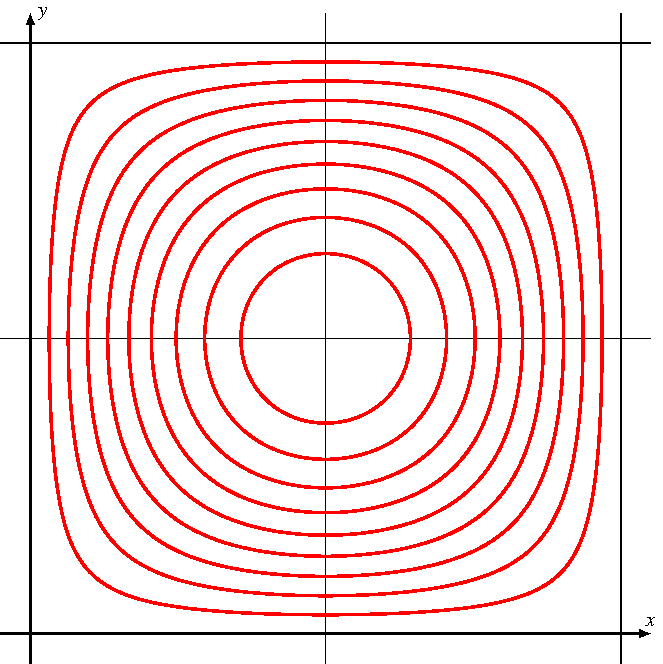
\includegraphics{chapters/2/konvektion.pdf}
\caption{Stromlinien in einer einzelnen Konvektionszelle
\label{skript:stromlinien konvektion}}
\end{figure}
Ausgehend von
\eqref{skript:lorenzausgangsgleichung}
versuchen wir nun, eine gewöhnliche Differentialgleichung zu gewinnen,
welche näherungsweise wiedergibt, was passiert, wenn im betrachteten
System Konvektion einsetzt.
Eine einzelne Konvektionszelle hat Stromlinien, wie sie in Abbildung
\ref{skript:stromlinien konvektion}
dargestellt sind.
Vernachlässigt man in der
ersten der Differentialgleichungen
\eqref{skript:lorenzausgangsgleichung}
$\vartheta$ und den nichtlinearen Term, bleibt eine Wärmeleitungsgleichung
für $\Delta \psi$
Die Wärmeleitungsgleichung auf einem Rechteckgebiet 
einer solchen Zelle könnte man mit einem Separationsansatz zu lösen
versuchen, dies würde auf Lösungen der Form
$\sin(ax)\sin(y)$
führen.
Wir versuchen daher eine Lösung für $\psi(x,y,t)$ in der etwas
allgemeineren Form
\begin{equation}
\psi(x,y,t)
=
X(t) \sin(ax)\sin(y)
\label{skript:psiansatz}
\end{equation}
zu finden.
Die Konvektion sorgt dafür, dass im Bereich grosser
Strömungsgeschwindigkeit der Temperaturgradient stark vom linearen Verlauf
abweicht.
Die vertikale Strömungsgeschwindigkeit ist bei $0$ und $\pi$ hoch, also
dort wo $\cos(ax)$ gross ist.
Wir setzen daher die Lösung für die Temperatur $\vartheta(x,y,t)$ an in der
Form
\begin{equation}
\vartheta(x,y,t)
=
Y(t) \cos(ax) \sin(y) - Z(t) \sin(2y).
\label{skript:thetaansatz}
\end{equation}
Das Ziel ist, für die drei Funktionen $X(t)$, $Y(t)$ und $Z(t)$
gewöhnliche Differentialgleichungen aufzustellen, also die Ortsabhängigkeit
der Lösungsfunktionen vollständig zu eliminieren.
Diese Technik heisst in der Theorie der partiellen Differentialgleichungen
auch die Transformationsmethode.

Wir können allerdings nicht erwarten, dass dies exakte Lösungen sind.
Beim Einsetzen in die Differentialgleichungen werden auch noch
andere Terme entstehen.
Unter der Annahme, dass die genannten Terme die Gestalt der Stromlinien
genau genug wiederzugeben in der Lage sind, vernachlässigen wir alle
Terme, die sich nicht als Vielfache der Funktionen
\begin{equation}
\sin(ax)\sin(y),
\qquad
\cos(ax)\sin(y)
\qquad\text{und}\qquad
\sin(2y)
\label{skript:funktionsauswahl}
\end{equation}
schreiben lassen.

Wir müssen jetzt also die Lösungsansatze
\eqref{skript:psiansatz}
und
\eqref{skript:thetaansatz}
in die Differentialgleichungen
\eqref{skript:lorenzausgangsgleichungen}
einsetzen.
Die linke Seite ist jeweils einfach, da die Zeitabhängigkeit nur noch
in den Funktion $X(t)$, $Y(t)$ und $Z(t)$ steckt.
Auf der linken Seite können wir daher einfach $X(t)$ durch $\dot X(t)$
ersetzen und analog für die anderen beiden Koeffizientenfunktionen.

Die Ortsableitungen geben etwas mehr zu tun:
\begin{align*}
\frac{\partial}{\partial x}\psi
&=
X(t)a\cos(ax)\sin(y)
&
\frac{\partial}{\partial y}\psi
&=
X(t)\sin(ax)\cos(y)
\\
\frac{\partial^2}{\partial x^2}\psi
&=
-X(t)a^2\sin(ax)\sin(y)
&
\frac{\partial^2}{\partial y^2}\psi
&=
-X(t)\sin(ax)\sin(y)
\\
\Delta\psi
&=-(a^2+1)\psi
&
\Delta^2 \psi
&=
(a^2+1)^2\psi.
\end{align*}
für $\psi$ und
\begin{align*}
\frac{\partial}{\partial x}\vartheta
&=
-aY(t) \sin(ax) \sin(y)
&
\frac{\partial}{\partial y}\vartheta
&=
Y(t) \cos(ax) \cos(y) - 2 Z(t)\cos(2y)
\\
\frac{\partial^2}{\partial x^2}\vartheta
&=
-a^2Y(t) \cos(ax) \sin(y)
&
\frac{\partial^2}{\partial y^2}\vartheta
&=
-Y(t) \cos(ax) \sin(y)
+4Z(t)\sin(2y)
\\
\Delta\vartheta
&=\mathrlap{-(a^2+1)Y(t)\cos(ax)\sin(y)+4Z(t)\sin(2y)}
\end{align*}
für $\vartheta$.
In den Differentialgleichungen brauchen wir aber noch die
Funktionaldeterminanten für die nichtlinearen Terme:
\begin{align*}
\frac{\partial(\psi,\Delta\psi)}{\partial(x,y)}
&=
\frac{\partial\psi}{\partial x} \frac{\partial\Delta\psi}{\partial y}
-
\frac{\partial\psi}{\partial y} \frac{\partial\Delta\psi}{\partial x}
=
-(a^2+1)\biggl(
\frac{\partial\psi}{\partial x} \frac{\partial\psi}{\partial y}
-
\frac{\partial\psi}{\partial y} \frac{\partial\psi}{\partial x}
\biggr)
=0
\\
\frac{\partial(\psi,\vartheta)}{\partial(x,y)}
&=
\frac{\partial\psi}{\partial x} \frac{\partial\vartheta}{\partial y}
-
\frac{\partial\psi}{\partial y} \frac{\partial\vartheta}{\partial x}
\\
&=
X(t)\biggl(
a \cos(ax)\sin(y)
\bigl(Y(t) \cos(ax) \cos(y) - 2Z(t)\cos(2y)\bigr)
\\
&\qquad
-
\sin(ax)\cos(y)
\bigl(-aY(t) \sin(ax) \sin(y) \bigr)
\biggr)
\\
&=
X(t)(a(\underbrace{\cos^2(ax)+\sin^2(ax)}_{\displaystyle=1})
Y(t)\underbrace{\sin(y)\cos(y)}_{\displaystyle{\textstyle\frac12}\sin(2y)}-2a\cos(ax)\sin(y)Z(t)\cos(2y))
\\
&=
\frac12aX(t)Y(t) \sin(2y)
-
2a X(t)Z(t) \cos(ax)\sin(y)\cos(2y)
\\
&=
\frac12aX(t)Y(t) \sin(2y)
-
2a X(t)Z(t) \cos(ax)\frac12(\sin(-y)+\sin(3y))
\\
&=
\frac12aX(t)Y(t) \sin(2y)
+
2aX(t)Z(t) \cos(ax)\sin(y)
-
2aX(t)Z(t) \cos(ax)\sin(3y).
\end{align*}
Der letzte Term kann nicht durch Funktionen aus der Liste
\eqref{skript:funktionsauswahl}
ausgedrückt werden, und muss daher vernachlässigt werden.
Setzen wir jetzt diese Ableitungen in die Differentialgleichungen
ein, erhalten wir
\begin{align*}
-(a^2+1)
\dot X(t) \sin(ax)\sin(y)
&=
\nu (a^2+1)^2 X(t)\sin(ax)\sin(y)
-acY(t)\sin(ax)\sin(y)
\\
\dot Y(t)\cos(ax)\sin(y)-\dot Z(t)\sin(2y)
&=
-\kappa (a^2+1)Y(t)\cos(ax)\sin(y) +4\kappa Z(t)\sin(2y)
\\
&\qquad +\frac{T_0}{\pi} X(t)a\cos(ax)\sin(y)
\\
&\qquad
-\frac{a}2X(t)Y(t)\sin(2y) - 2aX(t)Z(t)\cos(ax)\sin(y).
\end{align*}
Wir vergleichen die Koeffizienten der Funktionen aus der Liste
\eqref{skript:funktionsauswahl}
dann erhalten wir das Differentialgleichungssystem 

%(%i26)                               dglX
%             2       d                           4      2
%(%o26)   (- a  - 1) (-- (X(t))) + a c Y(t) + (- a  - 2 a  - 1) nu X(t)
%                     dt
%(%i27)                               dglY
%         a X(t) T_0   d                          2
%(%o27) - ---------- + -- (Y(t)) + a X(t) Z(t) + a  kappa Y(t) + kappa Y(t)
%            %pi       dt
%(%i28)                               dglZ
%                     d                          a X(t) Y(t)
%(%o28)             - -- (Z(t)) - 4 kappa Z(t) + -----------
%                     dt                              2

\begin{align*}
\dot X(t)
&=
-\nu(a^2+1)X(t)
+\frac{ac}{a^2+1}Y(t)
\\
\dot Y(t)
&=
\frac{aT_0}{\pi}X(t)
-(a^2+1)\kappa Y(t)
-aX(t)Z(t)
\\
\dot Z(t)
&=
-4\kappa Z(t)
+\frac{a}{2}X(t)Y(t)
\end{align*}
für die Koeffizientenfunktionen $X(t)$, $Y(t)$ und $Z(t)$.






	% 3
%
% fourier.tex -- oszillationsphänomene insbesondere Milankowitsch-Zyklern
%
% (c) 2018 Prof Dr Andreas Müller, Hochschule Rapperswil
%
\chapter{Fourier-Analysis\label{chapter:fourier}}
\lhead{Kapitel 6: Fourier-Analysis}
\rhead{ }
Im Kapitel~\ref{chapter:wetter und klima} wurde gezeigt, dass einige der
Einflüsse
auf das Klimasystem periodisch sind mit einer Periode, die vergleichbar
oder grösser ist als die bei der Definition des Begriffes Klima üblicherweise
verwendeten Mittelungszeitspanne.
Diese Anregungen führen daher zu periodischen Klimaschwankungen.
Die Fourier-Analysis ermögilcht, solche periodischen Einflüsse in
einem Signal zu erkennen und sie von anderen Phänomenen zu trennen.

%
% periodisch.tex -- periodische Funktionen
%
% (c) 2018 Prof Dr Andreas Müller, Hochschule Rapperswil
%
\section{Periodische Funktionen}
Das ursprüngliche Budyko-Modell modelliert die Jahresmitteltemperatur,
ignoriert also die Temperaturentwicklung der Temperatur im Laufe des
Jahres.
Damit ist es aber zum Beispiel nicht möglich, das Einsetzen von
Eiszeiten zu modellieren.
Die jährlich
auf die Erde eingetrahlte Energie ist unabhängig von der Neigung der
Erdachse.
Ein Modell, welches den Zusammenhang zwischen Eiszeiten und der
Achsneigung modellieren soll, muss also die periodischen Schwankungen
der Einstrahlung der Sonne auf jede Erd-Halbkugel berücksichtigen.

Ein geeignetes Modell wird also nicht mehr autonom sein, sondern auf der
rechten Seite der Differentialgleichung
\[
\frac{dx}{dt} = f(x,t)
\]
eine Funktion $f(x,t)$ haben, die nun auch von der Zeit $t$ abhängt
und periodisch in $t$ mit Periode $T$ ist.
Dies bedeutet $f(x,t+T)=f(x,t)$ für beliebige Vektoren $x$ und 
Zeiten $t$.
Die Periode muss nicht unbedingt genau ein Jahr sein, es sind auch
Vielfache eines Jahres denkbar.

Man kann natürlich nicht mehr erwarten, dass es eine zeitunabhängige
Gleichgewichtslösung gibt.
Vielmehr erwarten wir statt konstanter Gleichgewichtslösungen 
periodische Lösungen mit der gleichen Periode $T$, dass also
$x(t+T)=x(t)$.

\subsection{Fourierreihen}
Die Funktionen
\begin{equation}
1,\quad
\cos \frac{2\pi kt}{T},\quad
\sin \frac{2\pi kt}{T},\qquad k\in \mathbb N
\label{skript:periodisch:fourierbasis}
\end{equation}
sind alle periodisch mit Periode $T$, aber auch eine beliebige
Linearkombination
\begin{equation}
f(t)
=
a_0  +\sum_{k=1}^\infty\biggl(
a_k \cos \frac{2\pi kt}{T} + b_k\sin\frac{2\pi kt}{T}
\biggr),
\label{skript:periodisch:fourierreihe}
\end{equation}
ein sogenanntes trigonometrisches Polynom, hat diese Eigenschaft.
Damit lässt sich eine grosse Vielfalt von $2\pi$-periodischen
Funktionen wiedergeben.

Es war die bedeutende Erkenntnis von Joseph Fourier, dass bis auf ein
\index{Fourier, Joseph}%
paar technische Bedingungen, welche die Konvergenz der Funktionenreihe
\eqref{skript:periodisch:fourierreihe}
sicherstellen sollen, jede periodische Funktion $f(t)$ 
als Reihe von Vielfachen der Funktionen
\eqref{skript:periodisch:fourierbasis}
in der Form
\eqref{skript:periodisch:fourierreihe}
dargestellt werden kann.
Diese Bedingungen sind für stetige Funktionen immer erfüllt.
Die Berechnung der Koeffizienten $a_0,a_1,a_2,\dots$ und $b_1,b_2,b_3,\dots$
erfolgt mit Hilfe von Fourier-Integralen, deren Theorie wir hier weiter
nicht entwickeln wollen, wir kommen darauf in
Abschnitt~\ref{subsection:fourier:stetig} zurück.

Für unsere Zwecke ist die vollständige Theorie der Fourier-Reihen nicht
notwendig, denn die Daten, an die wir unsere Klimamodelle anpassen
müssen, stellen bestenfalls diskrete Approximationen von stetigen
Funktionen dar.
Wir müssen die allgemeine Fourier-Theorie daher spezialisieren auf diese
diskrete Situation.

\subsection{Diskrete Fourierreihen}
Wir wollen im Folgenden periodische diskrete Funktionen möglichst gut
approximieren.
Die Diskretisation wird charakterisiert durch die Anzahl
$N$ der bekannten Werte im Periodeninterval $[0,2\pi)$.

\subsubsection{Diskretisation}
Gegeben sind also die Werte $y_j$ einer $2\pi$-periodischen Funktion
$f(t)$ an den äquidistanten Stellen $t_j=2\pi j/N$ mit
$1\le j \le N$.
Da $f(t)$ eine $2\pi$-periodische Funktion ist, folgt
\[
y_j = f(t_j) = f(t_j+2\pi) = f(t_{j+N}).
\]
Wir erweitern daher die Notation für $y$ und setzen
\[
y_j = y_{r(j)},
\]
wobei $r(j)$ der Rest von $j$ bei Teilung durch $N$ steht.
Insbesondere ist $y_0=y_N$, die Folge $y_j$ ist $N$-periodisch als
Folge von reellen Zahlen.

\subsubsection{Trigonometrische Polynome}
Als Basis für die Darstellung der Funktion $f(t)$ verwenden wir
die bekanntermassen
$2\pi$-periodischen Funktionen 
\begin{equation}
1,\quad \cos kt\quad\text{und}\quad \sin kt,\qquad k\in\mathbb N.
\end{equation}
Die Funktion $f(t)$ soll also geschrieben werden als sogenanntes 
{\em trigonometrisches Polynom}
\index{trigonometrisches Polynom}%
\begin{equation}
f(t)
=
a_0 + \sum_{k=1}^n \bigl(a_k \cos kt + b_k\sin kt).
\label{skript:fourier:rekonstruktion}
\end{equation}
Ein Koeffizient $b_0$ ist nicht sinnvoll, weil die dazugehörige Basisfunktion
$\sin 0t =0$ ist.
Die Funktion $f(t)$ soll die Werte $y_j$
möglichst gut wiedergeben, es soll also wenn möglich $f(t_j) = y_j$ sein.

Zur Bestimmung der Koeffizienten $a_0$, $a_k$ und $b_k$ stehen genau
die $N$ Bedingungen
\begin{equation}
f(t_j)=y_j
\label{skript:periodisch:fourierbedingungen}
\end{equation}
zur Verfügung.
Die Gleichungen \eqref{skript:periodisch:fourierbedingungen} sind
lineare Gleichungen für die Unbekannten $a_k$ und $b_k$ mit
$\cos kt_j$ und $\sin kt_j$ als Koeffizienten.
Sie können daher höchstens $N$ der Koeffizienten $a_k$ und $b_k$
bestimmen.
Dieses Problem wird im nächsten Abschnitt gelöst.


%
% fourierkoef.tex -- Bestimmung der Fourier-Koeffizienten
%
% (c) 2018 Prof Dr Andreas Müller, Hochschule Rapperswil
%
\section{Fourier-Koeffizienten}
\rhead{Fourier-Koeffizienten}
In diesem Abschnitt bestimmen wir die Fourierkoeffizienten für ein
trigonometrisches Polynom der Form
\begin{equation}
p_n(t)
=
a_0 + \sum_{k=1}^{n-1} a_k\cos kt + \sum_{k=1}^{n-1} b_k\sin kt + a_n\cos nt,
\label{skript:fourier:ansatz}
\end{equation}
derart, dass die Werte
\begin{equation}
y_j \quad\text{zu den Zeitpunkten}\quad t_j=2\pi\frac{j}{N},\qquad 1\le j< N
\label{skript:fourier:gleichungen}
\end{equation}
möglichst genau die Funktionswerte $p_n(t_j)$ reproduzieren.

Im Ansatz~\eqref{skript:fourier:ansatz} für $p_n(t)$ finden wir
genau $2n$ zu bestimmende Koeffizienten, nämlich $a_0$,
$n$ Koeffizienten $a_k$ mit $k=1,\dots,n$
und $n-1$ Koeffizienten $b_k$ mit $k=1,\dots,n-1$.
Mit $N$ Datenpunkten $y_j$ haben wir genau die $N$ Bedingungen
$p_n(t_j)=y_j$, um diese Koeffizienten zu bestimmen.
Die Bedingungen $p_n(t_j)=y_j$ sind $N$ lineare Gleichungen für die
$2n$ Koeffizienten, sie dürften sich also genau dann exakt lösen
lassen, wenn $N=2n$, wenn also die Zahl der Datenpunkte gerade ist.

Für $N<2n$ haben wir weniger Gleichungen als Koeffizienten, es ist
also unmöglich, die Koeffizienten ohne zusätzliche Annahmen zu bestimmen.
Das Problem ist also nur dann überhaupt lösbar, wenn $N\ge 2n$ ist.
Für $N>2n$ haben wir zu viele Daten, wir können nicht erwarten, dass
das Gleichungssystem $p_n(t_j)=y_j$ überhaupt eine Lösung hat.
Im optimalen Fall, für $N=2n$ sollte es möglich sein, die Koeffizienten so
zu bestimmen, dass die Funktionswerte $y_j$ exakt reproduziert werden.

\subsection{Least Squares}
Für $N>2n$ können wir nicht erwarten, dass der Ansatz
\eqref{skript:fourier:ansatz} die Daten exakt reproduzieren kann,
wir müssen uns also mit einer Näherungslösung begnügen.
Wir verlangen stattdessen, dass der Fehler der Lösung möglichst gering
wird, dass also
\[
L=L(a_0,a_1,\dots,a_n,b_1,\dots,b_{n-1})= \sum_{j=1}^N (y_j - p_n(t_j))^2
\]
möglichst klein wird.

Die Grösse $L$ wird minimal, wenn alle Ableitungen nach den Koeffizienten
verschwinden:
\begin{equation}
\frac{\partial L}{\partial a_0}=0,
\qquad
\frac{\partial L}{\partial a_l}=0, \;{1\le l\le n}
\qquad
\frac{\partial L}{\partial b_l}=0, \;{1\le l\le n-1}
\label{skript:fourier:leastsquaresableitungen}
\end{equation}
Um die Koeffizienten zu bestimmen, müssen wir die Ableitungen in
\eqref{skript:fourier:leastsquaresableitungen}
berechnen und erhalten die Gleichungen
\begin{align}
\frac{\partial L}{\partial a_0}
&=
-2 \sum_{j=1}^N (y_j-p_n(t_j))\cdot \frac{\partial p_n}{\partial a_0}(t_j)=0,
&&
\label{skript:fourier:a0ableitung}
\\
\frac{\partial L}{\partial a_l}
&=
-2 \sum_{j=1}^N (y_j-p_n(t_j))\cdot \frac{\partial p_n}{\partial a_l}(t_j)=0
&k&=1,\dots,n,
\label{skript:fourier:akableitung}
\\
\frac{\partial L}{\partial b_l}
&=
-2 \sum_{j=1}^N (y_j-p_n(t_j))\cdot \frac{\partial p_n}{\partial b_l}(t_j)=0
&k&=1,\dots,n-1.
\label{skript:fourier:bkableitung}
\end{align}
Man beachte, dass $p_n(t_j)$ die Koeffizienten $a_0$, $a_k$ und $b_k$
linear enthält.
Der erste Klammerausdruck $y_j-p_n(t_j)$ in der Summe enthält daher die
Koeffizienten ebenfalls nur linear, die Ableitungen nach den Koeffizienten
enhalten daher die Koeffizienten überhaupt nicht mehr.
Tatsächlich ergibt die Berechnung der Ableitungen
\begin{align}
\frac{\partial p_n}{\partial a_0}(t_j)
&=
1
&&
\label{skript:fourier:a0abl}
\\
\frac{\partial p_n}{\partial a_l}(t_j)
&=
\cos lt_j
&l&=1,\dots,n
\label{skript:fourier:akabl}
\\
\frac{\partial p_n}{\partial b_l}(t_j)
&=
\sin lt_j
&l&=1,\dots,n-1.
\label{skript:fourier:bkabl}
\end{align}
\definecolor{darkblue}{rgb}{0,0,0.6}%
Setzen wir diese Ableitungen als {\color{darkblue}dunkelblaue} Terme in
\eqref{skript:fourier:a0ableitung}--\eqref{skript:fourier:bkableitung} ein
und vertauschen die Reihenfolge der Summationen über $k$ und $j$,
erhalten wir die Gleichungen
\definecolor{darkred}{rgb}{0.6,0,0}%
\begin{equation}
\left.
\begin{aligned}
0&=
\sum_{j=1}^N
\biggl(
y_j - a_0 - \sum_{k=1}^n a_k\cos kt_j - \sum_{k=1}^{n-1} b_k\sin kt_j
\biggr)\cdot\mathstrut{\color{darkblue}1}
\\
&=
\sum_{j=1}^N y_j
-Na_0
-\sum_{k=1}^n a_k {\color{darkred}\sum_{j=1}^N\cos kt_j}
-\sum_{k=1}^{n-1} b_k {\color{darkred}\sum_{j=1}^N\sin kt_j},
\\
0&=
\sum_{j=1}^N
\biggl(
y_j - a_0 - \sum_{k=1}^n a_k\cos kt_j - \sum_{k=1}^{n-1} b_k\sin kt_j
\biggr)\cdot\mathstrut {\color{darkblue}\cos lt_j}
\\
&=
\sum_{j=1}^N y_j \cos lt_j
-a_0\sum_{j=1}^N \cos lt_j
-\sum_{k=1}^n a_k {\color{darkred}\sum_{j=1}^N\cos kt_j\cos lt_j}
-\sum_{k=1}^{n-1} b_k {\color{darkred}\sum_{j=1}^N\sin kt_j\cos lt_j},
%&l&=1,\dots,n-1
\\
0
&=
\sum_{j=1}^N
\biggl(
y_j - a_0 - \sum_{k=1}^n a_k\cos kt_j \sum_{k=1}^{n-1} b_k\sin kt_j
\biggr)\cdot\mathstrut {\color{darkblue}\sin lt_j}
\\
&=
\sum_{j=1}^N y_j \sin lt_j
-a_0\sum_{j=1}^N \sin lt_j
-\sum_{k=1}^n a_k {\color{darkred}\sum_{j=1}^N\cos kt_j\sin lt_j}
-\sum_{k=1}^{n-1} b_k {\color{darkred}\sum_{j=1}^N\sin kt_j\sin lt_j}.
%&l&=1,\dots,n
\end{aligned}
\right\}
\label{skript:fourier:gl2}
\end{equation}
Hier haben wir die Faktoren $-2$ ebenfalls weggelassen.
Auf den ersten Blick scheinen diese Gleichungen nicht einfach lösbar zu
sein, die {\color{darkred}dunkelrot} hervorgehobenen Koeffizienten der
Unbekannten $a_0$, $a_k$ und $b_k$ scheinen ziemlich kompliziert zu sein.
Es stellt sich aber heraus, dass diese direkt ausgewertet werden können,
was im nächsten Abschnitt geschehen soll.

\subsection{Trigonometrische Summen}
In den Gleichungen~\eqref{skript:fourier:gl2} treten als Koeffizienten
für die Unbekannteno $a_0$, $a_k$ und $b_k$ trigonometrische Summen
der Form
\begin{equation}
\sum_{j=1}^N \cos kt_j
\qquad
\text{oder}
\qquad
\sum_{j=1}^N \sin kt_j,
\label{skript:fourier:trigosum}
\end{equation}
sowie Summen von Produkten trigonmetrischer Funktionen wie
\begin{equation}
\sum_{j=1}^N \cos kt_j\cos lt_j,\quad
\sum_{j=1}^N \cos kt_j\sin lt_j
\quad
\text{oder}
\quad
\sum_{j=1}^N \sin kt_j\sin lt_j
\label{fourier:produkte}
\end{equation}
auf.
In diesem Abschnitt sollen diese Summen mit Hilfe einer geometrischen
Überlegung berechnet werden.

Wir befassen uns zunächst mit Summen der Form
\eqref{skript:fourier:trigosum} und beweisen den folgenden Satz.

\begin{figure}
\centering
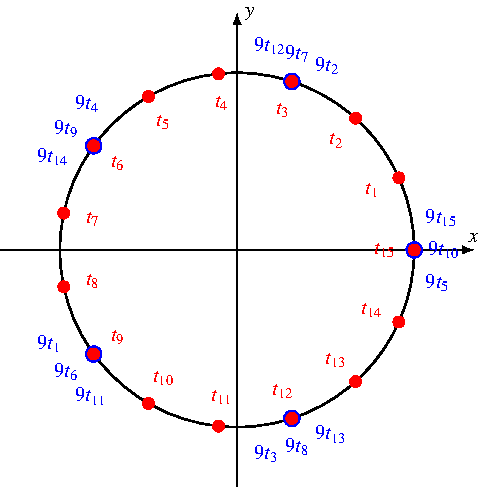
\includegraphics{chapters/6/trigosum.pdf}
\caption{Verteilung der Punkte $(\cos t_j, \sin t_j)$  auf dem Einheitskreis 
in rot.
Die Punkte $(\cos kt_j,\sin kt_j)$ für $k=9$ bilden eine Teilmenge, die
blau dargestellt ist.
Jeder blaue Punkt wird genau dreimal besucht, sie bilden ein gleichseitiges
Fünfeck mit den Punkten $(\cos 3t_j,\sin 3t_j)$ als Ecken.
Deren Schwerpunkt ist wieder der Nullpunkt.
\label{fourier:einheitskreis}
}
\end{figure}

\begin{satz}
\label{skript:fourier:orthogonalitaet1}
Ist $t_j=2\pi j/N$, dann gelten für beliebige ganze Zahlen $l$,
mit $0\le l\le n$, die Identitäten
\begin{equation*}
\begin{aligned}
\sum_{j=1}^N \cos lt_j
&=
\begin{cases}
N&\qquad l=0\\
0&\qquad\text{sonst}
\end{cases}
\\
\sum_{j=1}^N \sin lt_j
&=0.
\end{aligned}
\end{equation*}
\end{satz}

\begin{proof}[Beweis]
Wir betrachten zunächst den Fall $l=0$.
In diesem Fall ist $\cos lt_j=1$ und $\sin lt_j=0$ und damit
\[
\sum_{j=1}^N \cos lt_j = N
\qquad\text{und}\qquad
\sum_{j=1}^N \sin lt_j = 0.
\]
Im Folgenden können wir daher annehmen, dass $l\ne 0$.

In Abbildung~\eqref{fourier:einheitskreis} kann man sehen, dass die Punkte
$(\cos t_j,\sin t_j)$ auf dem Einheitskreis ein regelmässiges Polygon
mit $N$ Ecken bilden.
Der Schwerpunkt des Polygons ist ganz offensichtlich der Mittelpunkt.
Daraus folgt
\[
\sum_{j=1}^N \cos t_j = 0
\qquad\text{und}\qquad
\sum_{j=1}^N \sin t_j = 0.
\]
Damit ist der Satz für den Fall $l=1$ bewiesen.

Für beliebiges $l\ne 0$ beobachten wir, dass die Punkte 
$(\cos lt_j,\sin lt_j)$ eine Teilmenge der Punkte $(\cos t_j, \sin t_j)$
sind.
Wenn $l$ und $N$ teilerfremd sind, sind die Mengen gleich.
Wenn $l$ und $N$ dagegen den grössten gemeinsamen Teiler
$r=\operatorname{ggT}(l,N)$ haben, dann
ist die Menge 
\[
\{ 
(\cos lt_j,\sin lt_j)\,|\,j=1,\dots,N
\}
=
\{
(\cos rt_j,\sin rt_j)\,|\,j=1,\dots,N/r
\}
\]
ein regelmässiges Polygon mit $N/r$ Ecken.
Diese Situation ist in Abbildung~\ref{fourier:einheitskreis} mit den
blauen Punkten für den Fall $r=3=\operatorname{ggT}(9,15)$
illustriert.
Wie im Falle von $l=1$ folgt\footnote{Etwas formeller könnten wir sagen,
dass wir hier vollständige Induktion nach $N$ machen.
Was wir im letzten Schritt nämlich brauchen ist der Wert einer
trigonometrischen Summe mit $N/r<N$ Summanden, deren Werte wir gemäss
der naheligenden Induktionsannahme bereits kennen.},
dass der Schwerpunkt des Polygons der
Nullpunkt ist, und damit, dass
\begin{align*}
\sum_{j=1}^N \cos lt_j 
=
\sum_{j=1}^N \cos rt_j 
=
0,
\\
\sum_{j=1}^N \sin lt_j 
=
\sum_{j=1}^N \sin rt_j 
=
0.
\end{align*}
Damit ist alles gezeigt.
\end{proof}

In \eqref{fourier:produkte} werden die Summen von Produkten benötigt.
Mit üblichen trigonometrischen Umformungen kann man diese in Summen
von einfachen trigonometrischen Funktionen umwandeln.
Wir verwenden dazu die Formeln
\begin{align}
\cos\alpha\cos\beta
&=
\frac12\bigl(\cos(\alpha-\beta)+\cos(\alpha+\beta)\bigr),
\label{fourier:coscos}
\\
\sin\alpha\sin\beta
&=
\frac12\bigl(\cos(\alpha-\beta) + \cos(\alpha+\beta)\bigr).
\label{fourier:sinsin}
\\
\sin\alpha\cos\beta
&=
\frac12\bigl(\sin(\alpha-\beta) + \sin(\alpha+\beta)\bigr),
\label{fourier:sincos}
\end{align}
Damit können wir die Summen in \eqref{fourier:produkte} umwandeln:
\begin{align*}
\sum_{j=1}^N \cos kt_j\cos lt_j
&=
\sum_{j=1}^N \frac12\bigl(\cos (k-l)t_j +\cos(k+l)t_j\bigr)
\\
&=
\frac12\sum_{j=1}^N \cos (k-l)t_j
+ \frac12\underbrace{\sum_{j=1}^N\cos(k+l)t_j}_{\displaystyle=0}
\\
&=
\begin{cases}
\displaystyle\frac{N}2&\qquad k=l\\
0&\qquad\text{sonst}
\end{cases}
\\
\sum_{j=1}^N \sin kt_j \sin lt_j
&=
\sum_{j=1}^N \frac12\bigl(\cos(k-l)t_j +\cos(k+l)t_j\bigr)
\\
&=\frac12\sum_{j=1}^N \cos(k-l)t_j
+\frac12\underbrace{\sum_{j=1}^N \cos(k+l)t_j}_{\displaystyle=0}
\\
&=
\begin{cases}
\displaystyle\frac{N}2&\qquad k=l\\
0&\qquad\text{sonst}
\end{cases}
\\
\sum_{j=1}^N \sin kt_j \cos lt_j
&=
\sum_{j=1}^N \frac12\bigl(\sin(k-l)t_j +\sin(k+l)t_j\bigr)
\\
&=
\frac12\underbrace{\sum_{j=1}^N \sin(k-l)t_j}_{\displaystyle=0}
+
\frac12\underbrace{\sum_{j=1}^N \sin(k+l)t_j}_{\displaystyle=0}
=0.
\end{align*}
Damit haben wir den folgenden Satz bewiesen:

\begin{satz}
\label{skript:fourier:satzprodukte}
Für beliebige $k,l\in \mathbb N$ gilt
\begin{align*}
\sum_{j=1}^N
\cos kt_j \cos lt_j
&=
\begin{cases}
N                     &\qquad k=l=0\\
\displaystyle\frac{N}2&\qquad k=l > 0\\
0                     &\qquad\text{sonst}
\end{cases}
\\
\sum_{j=1}^N
\sin kt_j \sin l_j
&=
\begin{cases}
\displaystyle \frac{N}2&\qquad k=l\\
0                      &\qquad\text{sonst}
\end{cases}
\\
\sum_{j=1}^N
\sin kt_j \cos lt_j
&=
0
\end{align*}
\end{satz}
Mit dem Kronecker-$\delta$ 
\index{Kronecker-$\delta$}%
\[
\delta_{kl}
=
\begin{cases}
1&\qquad k=l\\
0&\qquad\text{sonst}
\end{cases}
\]
können wir die ersten zwei Formeln für $k,l>0$ noch etwas kompakter 
als
\begin{equation}
\sum_{j=1}^N
\cos kt_j \cos lt_j
=
\sum_{j=1}^N
\sin kt_j \sin l_j
=
\delta_{kl}\frac{N}2
\label{skript:fourier:trigsumsummary}
\end{equation}
schreiben.

In den folgenden Abschnitten verwenden wir diese Formeln, um die
Koeffizienten $a_k$ und $b_k$ zu bestimmen.
Der Koeffizient $a_0$ muss gesondert behandelt werden.

\subsection{Bestimmung von $a_0$}
In der Gleichung
\[
0
=
\sum_{j=1}^Ny_j
-Na_0
-\sum_{k=1}^na_k\underbrace{\sum_{j=1}^N\cos kt_j}_{\displaystyle=0}
-\sum_{k=1}^nb_k\underbrace{\sum_{j=1}^N\sin kt_j}_{\displaystyle=0}
\]
verschwinden die trigonometrischen Summen über $j$ nach
Satz~\ref{skript:fourier:orthogonalitaet1} und es bleibt die Gleichung
\begin{align*}
0
&=
\sum_{j=1}^Ny_j
-Na_0
\\
\Rightarrow\qquad
a_0&=\frac1{N}\sum_{j=1}^N y_j.
\end{align*}
Der Koeffizient $a_0$ ist der Mittelwert der Werte $y_j$.

\subsection{Bestimmung von $a_k, k>0$}
Zur Bestimmung von $a_k$ mit $k>0$ müssen wir die Gleichung
\[
0
=
\sum_{j=1}^N y_j\cos lt_j
-
a_0\underbrace{\sum_{j=1}^N\cos lt_j}_{\displaystyle=0}
-\sum_{k=1}^na_k\sum_{j=1}^N\cos kt_j\cos lt_j
-\underbrace{\sum_{k=1}^nb_k\sum_{j=1}^N\sin kt_j\cos lt_j}_{\displaystyle=0}
\]
heranziehen.
Die zweite und vierte Summe verschwindet wegen
Satz~\ref{skript:fourier:satzprodukte}, so dass wir die die Gleichung
\begin{align*}
0&=
\sum_{j=1}^N y_j\cos lt_j
-\sum_{k=1}^na_k\sum_{j=1}^N\cos kt_j\cos lt_j
\end{align*}
erhalten.
Die innere Summe über $j$ im zweiten Term verschwindet, wieder gemäss 
Satz~\ref{skript:fourier:satzprodukte}, für alle Werte
von $k$ ausser für $k=l$, in diesem Fall ist sie $N/2$. 
Damit können wir nach $a_k$ auflösen:
\begin{align*}
0&
=
\sum_{j=1}^N y_j\cos lt_j
-\sum_{k=1}^na_k\delta_{kl}\frac{N}2
=
\sum_{j=1}^N y_j\cos lt_j
-a_l\frac{N}2
\\
\Rightarrow\qquad 
a_l &= \frac{2}{N}\sum_{j=1}^Ny_j\cos lt_j.
\end{align*}

\subsection{Bestimmung von $b_k$}
Zur Bestimmung von $b_k$ müssen wir die Gleichung
\[
0=\sum_{j=1}^N y_j\sin lt_j 
-a_0\sum_{j=1}^N \sin lt_j
-\sum_{k=1}^na_k\sum_{j=1}^N\cos kt_j\sin lt_j
-\sum_{k=1}^nb_k\sum_{j=1}^N\sin kt_j\sin lt_j
\]
heranziehen.
Nach Satz~\ref{skript:fourier:satzprodukte}
verschwindet die zweite und die dritte Summe 
und in der letzten Summe
verschwinden alle Terme ausser der Term mit $k=l$, für den die
innere Summe über $j$ den Wert $N/2$ hat.
Damit wird die Gleichung vereinfacht zu
\begin{align*}
0
&=
\sum_{j=1}^Ny_j\sin lt_j - \sum_{k=1}^{n-1}b_l\delta_{kl}\frac{N}2
=
\sum_{j=1}^Ny_j\sin lt_j - b_l\frac{N}2
\\
\Rightarrow\qquad
b_l
&=
\frac{2}{N}\sum_{j=1}^Ny_j\sin lt_j.
\end{align*}

\subsection{Zusammenstellung der Resultate}
Sei $N=2n$ eine gerade natürliche Zahl.
Eine $2\pi$-periodische Funktion $f(t)$ kann als trigonometrisches Polynom
der Form
\[
p_n(t)
=
a_0 + \sum_{k=1}^{n-1} (a_k\cos kt + b_k\sin kt) + a_n\cos nt
\]
derart approximiert werden, dass zu den Zeiten $t_j=2\pi j/N, j=1,\dots,N$ 
die Funktion und das trigonometrische Polynom übereinstimmen:
\[
f(t_j) = y_j = p_n(t_j).
\]
Dazu müssen die Koefizienten
\begin{align*}
a_0
&=
\frac{1}N
\sum_{j=1}^N y_j,
\\
a_k
&=
\frac{2}N
\sum_{j=1}^N y_j\cos t_j
=
\frac{2}N
\sum_{j=1}^N y_j\cos \frac{2\pi j}{N}&\text{für }k&=1,\dots,n
\\
\text{und}\qquad
b_k
&=
\frac{2}N
\sum_{j=1}^N y_j\sin t_j
=
\frac{2}N
\sum_{j=1}^N y_j\sin \frac{2\pi j}{N}&\text{für }k&=1,\dots,n-1,
\end{align*}
verwendet werden.

\subsection{Beispiel: Dreiecksfunktion}
\begin{figure}
\centering
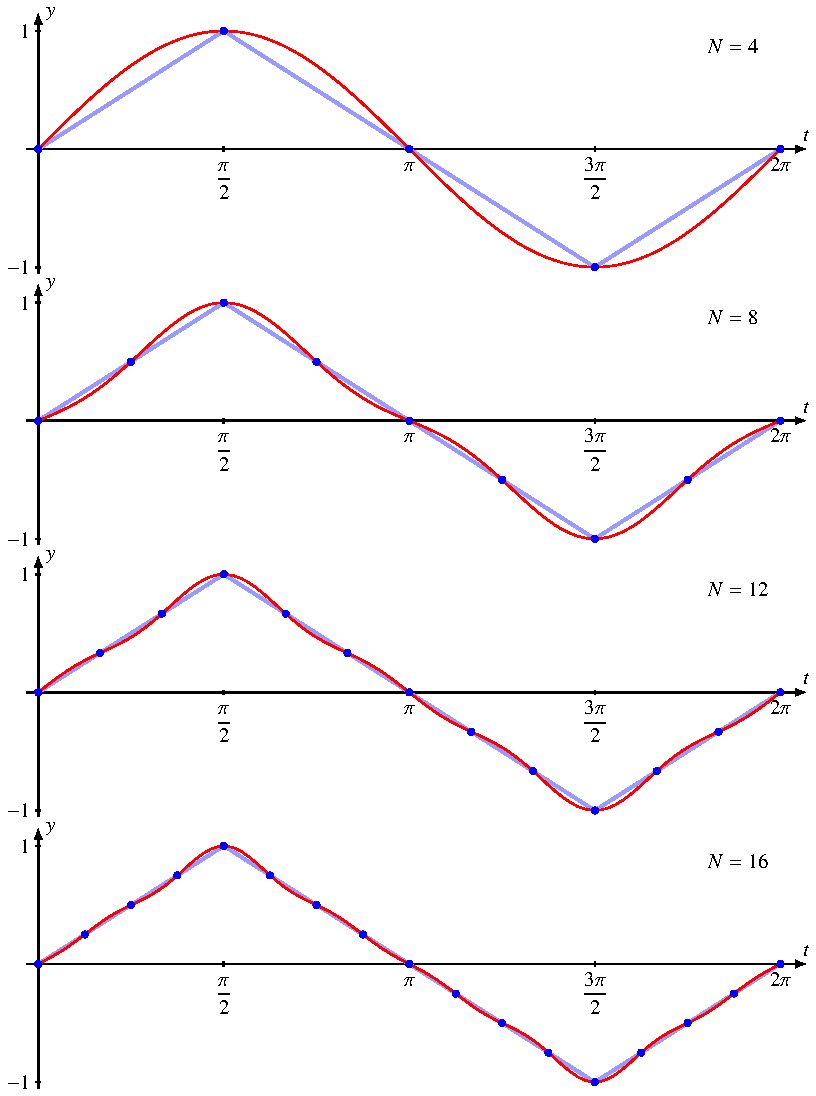
\includegraphics{chapters/6/dreieck.pdf}
\caption{Dreiecksfunktion ({\color{blue}blau}) approximiert mit
trigonometrischen Polynomen  $p_n(t)$ ({\color{red}rot})
mit verschiedenen Werten von $N=2n$.
\label{skript:fourier:beispiel}}
\end{figure}
\begin{table}
\centering
\setlength{\tabcolsep}{5pt}
\begin{tabular}{>{$}l<{$}>{$}r<{$}>{$}r<{$}>{$}r<{$}>{$}r<{$}>{$}r<{$}>{$}r<{$}>{$}r<{$}>{$}r<{$}}
&N=4&N=8&N=12&N=16&N=20&N=24&\dots&N=\infty\\
\hline
b_1&1& 0.85355& 0.82934& 0.82107& 0.81727& 0.81522&& 0.8105695\\
b_3& &-0.14645&-0.11111&-0.10124&-0.09704&-0.09484&&-0.0900633\\
b_5& &        & 0.05954& 0.04520& 0.04000& 0.03748&& 0.0324228\\
b_7& &        &        &-0.03249&-0.02519&-0.02207&&-0.0165422\\
b_9& &        &        &        & 0.02050& 0.01627&& 0.0100070\\
b_{11}&&      &        &        &        &-0.01413&&-0.0066989\\
%\hline
\end{tabular}
\caption{Nicht verschwindende Fourier-Koeffizienten der
Dreiecksfunktion~\eqref{skript:fourier:dreieck}
für verschiedene Werte von $N$.
In der Spalte ganz rechts unter $N=\infty$ die Werte für die
Fourierkoeffizienten der stetigen Fourier-Reihe
nach \eqref{fourier:normalekoeffizienten}.
\label{skript:fourier:dreieckkoef}}
\end{table}
Als Beispiel untersuchen wir die Approximation der
$2\pi$-periodischen Dreiecksfunktion, die auf dem Interval $[0,2\pi)$
durch
\begin{equation}
f(t)
=
\begin{cases}
\displaystyle t\cdot\frac{2}{\pi}    &\displaystyle \qquad 0\le t < \frac{\pi}2\\[8pt]
\displaystyle 2-t\cdot\frac{2}{\pi}  &\displaystyle \qquad \frac{\pi}2\le t < \frac{3\pi}2\\[8pt]
\displaystyle t\cdot\frac{2}{\pi} - 4&\displaystyle \qquad \frac{3\pi}2\le t <2\pi
\end{cases}
\label{skript:fourier:dreieck}
\end{equation}
gegeben ist,
mit Hilfe eines trigonometrischen Polynoms.
In Abbildung~\ref{skript:fourier:beispiel} ist die Dreiecksfunktion
hellblau dargestellt.

Weil die Funktion antisymmetrisch ist, verschwinden alle $a_k$-Koeffizienten.
Da die Funktion ausserdem symmetrisch ist bezüglich $\frac{\pi}2$ verschwinden
alle geraden $b_k$-Koeffizienten.
Für $N=4$ besteht $y$ nur aus vier Werten: $1$, $0$, $-1$ und $0$,
in diesem Fall muss die Funktion mit nur einem einzigen $\sin$-Term
mit dem Fourier-Koeffizienten $b_1$ darstellbar sein.
Tatsächlich ist $f(t) = \sin t$ an den Stellen $t_j=2\pi j/4$, $j=1,\dots,4$
(blau in Abbildung~\ref{skript:fourier:beispiel}),
dies wird in Abbildung~\ref{skript:fourier:beispiel} ganz oben gezeigt.
Erhöht man $N$, wird die Approximation immer besser, dies zeigen die
weiteren Graphiken in Abbildung~\ref{skript:fourier:beispiel}.

Die Berechnung der Fourier-Koeffizienten mit den Integralformeln
\eqref{fourier:normalekoeffizienten}
liefert für die Dreiecksfunktion~\eqref{skript:fourier:dreieck}
die Formel
\[
b_k = (-1)^{(k-1)/2}\frac{8}{\pi^2k^2}
\]
für ungereade Werte von $k$.
Diese Werte sind in der letzten Spalte unter $N=\infty$ dargestellt.
Für zunehmendes $N$ konvergieren die diskreten Koeffizienten $b_k$ gegen 
diese stetigen Werte.


%
% vektorgeometrie.tex
%
% (c) 2018 Prof Dr Andreas Müller, Hochschule Rapperswil
%
\section{Vektorgeometrische Interpretation}
\rhead{Vektorschreibweise}
Die bisherigen rein analytischen Betrachtungen verdecken den geometrischen
Gehalt der bisher entwickelten Theorie.
In diesem Abschnitt soll daher zunächst eine vektorielle Darstellung
aufgebaut, die dann erlauben soll, einerseits die Formeln für die 
Fourierkoeffizienten geometrisch zu verstehen und andererseits auf
komplexere Situationen zu verallgemeinern.

\subsection{Vektoren}
Die Operationen zur Bestimmung der Fourier-Koeffizienten können in 
vektorieller Schreibweise etwas übersichtlicher dargestellt werden.
Zunächst fassen wir die Funktionswerte $y_j$ in einem Vektor zusamen.
\begin{equation}
y = \begin{pmatrix}y_1\\\vdots\\y_N\end{pmatrix}
\end{equation}
Zur Berechnung der Fourier-Koeffizienten brauchen wir auch noch die
Werte der trigonometrischen Funktionen zu den Zeiten $t_j$, die wir
ebenfalls als Vektoren
\begin{align*}
c_0&=\begin{pmatrix}0\\\vdots\\0\end{pmatrix},
&
c_k&=\begin{pmatrix}\cos kt_1\\\vdots\\\cos kt_N\end{pmatrix},\;(k=1,\dots,n)
&&\text{und}
&
s_k&=\begin{pmatrix}\sin kt_1\\\vdots\\\sin kt_N\end{pmatrix},\;(k=1,\dots,n-1)
\end{align*}
schreiben.
Die Fourier-Koeffizienten können jetzt als Skalarprodukte geschrieben werden:
\begin{align*}
a_0 &=\frac1N c_0\cdot y,&
a_k &=\frac2N c_k\cdot y,\;(k=1,\dots,n),&
b_k &=\frac2N s_k\cdot y,\;(k=1,\dots,n-1).
\end{align*}

\subsubsection{Rekonstruktion der Funktion}
Auch die Darstellung der Funktion kann man wieder als Skalarprodukt schreiben.
Dazu schreiben wir die Fourier-Koeffizienten und die Werte der
trigonometrischen Funtionen also Vektoren
\begin{align*}
a
&=
\begin{pmatrix}
a_0\mathstrut\\
a_1\mathstrut\\
b_1\mathstrut\\
a_2\mathstrut\\
b_2\mathstrut\\
\vdots\\
b_{n-1}\mathstrut\\
a_n\mathstrut
\end{pmatrix}
&&\text{und}
&
e(t)
&=
\begin{pmatrix}
1\\
\cos t\\
\sin t\\
\cos2t\\
\sin2t\\
\vdots\\
\sin(n-1)t\\
\cos nt
\end{pmatrix}.
\end{align*}
Damit wird 
\[
p(t) = a\cdot e(t)
\]

\subsubsection{Orthogonalität}
Die Aussagen von Satz~\ref{skript:fourier:orthogonalitaet1}
lassen sich jetzt in geometrische Form fassen.
\begin{satz}
Es gilt
\begin{align*}
c_k\cdot c_l
&=
\begin{cases}
N&\qquad k=l=0\\
\displaystyle\frac{N}2&\qquad k=l>0\\
0&\qquad\text{sonst}
\end{cases}
\\
s_k\cdot s_l
&=
\begin{cases}
\displaystyle\frac{N}2&\qquad k=l\\
0&\qquad\text{sonst}
\end{cases}
\\
c_k\cdot s_l
&=
0
\end{align*}
\label{skript:fourier:orthogonalitaet}
\end{satz}

\begin{proof}[Beweis]
Die genannten Skalarprodukte sind nichts anderes als die Summen in
Satz~\ref{skript:fourier:orthogonalitaet1}:
\begin{align*}
c_k\cdot c_l
&=
\sum_{j=1}^N \cos kt_j \cos lt_j
=
\begin{cases}
N&\qquad k=l=0\\
\displaystyle\frac{N}2&\qquad k=l>0\\
0&\qquad\text{sonst}
\end{cases}
\end{align*}
und analog für die anderen Skalarprodukte.
Die Aussage des Satzes ist daher nichts anders als eine geometrische
Umformulierung der Aussagen des
Satzes~\ref{skript:fourier:orthogonalitaet1}.
\end{proof}

\subsubsection{Die Identität von Parseval}
Die Relationen von
Satz~\ref{skript:fourier:orthogonalitaet1}
besagen, dass die Vektoren $c_k$ und $s_k$ orthogonal sind.
Wir wenden Sie auf das Skalarprodukt der Funktion $f$ mit sich selbst an.
\begin{align*}
f\cdot f
&=
a_0^2 c_0\,\cdot c_0
+
\sum_{k=1}^na_k^2 \,c_k\cdot c_k
+
\sum_{k=1}^{n-1} b_k^2\,s_k\cdot s_k
\\
&=
Na_0^2
+
\frac{N}2\sum_{k=1}^n a_k^2
+
\frac{N}2\sum_{k=1}^{n-1} b_k^2
=
\frac{N}2
\biggl(
2a_0^2
+
\sum_{k=1}^n a_k^2
+
\sum_{k=1}^{n-1} b_k^2
\biggr)
\end{align*}
Damit haben wir den folgenden Satz bewiesen:
\begin{satz}[Parseval]
\[
\|f\|^2
=
\sum_{j=1}^N y_j^2
=
\frac{N}2
\biggl(
2a_0^2
+
\sum_{k=1}^n a_k^2
+
\sum_{k=1}^{n-1} b_k^2
\biggr)
\]
\end{satz}

\subsubsection{$2\pi$-Periodische Funktionen auf $\mathbb R$}
Die eben vektoriell dargestellte Analyse diskreter periodischer Funktionen 
kann verallgemeinert werden auf die Analyse von Funktionen auf
anderen Definitionsgebieten.
Benötigt wird eine Familie von Basisfunktionen und ein Skalarprodukt
$\langle\;,\;\rangle$ derart, dass die Basisfunktionen $g_i$ bezüglich
dieses Skalarproduktes orthonormiert sind, dass also
\[
\langle g_i,g_j\rangle
=
\delta_{ij}
=
\begin{cases}
1&\qquad i=j\\
0&\qquad\text{sonst}.
\end{cases}
\]
Jede Linearkombination
\[
f = \sum_{i} \alpha_i g_i
\]
von Basisfunktionen kann ebenfalls mit dem Skalarprodukt rekonstruiert
werden.
Dazu berechnet man
\[
\langle g_i,f\rangle
=
\biggl\langle
g_i,\sum_j\alpha_jg_j
\biggr\rangle
=
\sum_j \langle g_i,\alpha_jg_j\rangle
=
\sum_j \alpha_j\delta_{ij}
=
\alpha_i.
\]
Das Skalarprodukt kann auch verwendet werden, um einen Abstand zwischen
Vektoren als
\[
\| f-g\|^2
=
\langle f-g,f-g\rangle
\]
zu definieren.

Dieselbe Situation lässt sich auch für $2\pi$-periodische Funktionen 
auf $\mathbb R$ herbeiführen.
Als Basisfunktionen kann man die Funktionen 
\begin{equation}
\frac{1}{\sqrt{2}},\; \cos kx,\; \sin lx\quad k>0
\label{fourier:basis}
\end{equation}
verwenden.
Das Skalarprodukt $\langle f,g\rangle$ muss linear in $f$ und $g$ sein.
Eine naheliegende Wahl ist
\[
\langle f, g\rangle
=
\frac{1}{\pi}\int_{-\pi}^{\pi} f(x)\,g(x)\,dx.
\]
Wir überprüfen, ob die Funktionen orthogonal sind:
\begin{align*}
\left\langle \frac1{\sqrt{2}},\frac1{\sqrt{2}}\right\rangle
&=
\frac1{\pi}
\int_{-\pi}^{\pi} \frac12\,dx
=
1
\\
\left\langle \frac1{\sqrt{2}},\cos kx\right\rangle
&=
\frac1{\pi}\int_{-\pi}^{\pi}
\frac1{\sqrt{2}}\cos kx
\,dx
=0
\\
\left\langle \frac1{\sqrt{2}},\sin kx\right\rangle
&=
\frac1{\pi}\int_{-\pi}^{\pi}
\frac1{\sqrt{2}}\sin kx
\,dx
=0
\\
\langle \cos kx,\cos lx\rangle
&=
\frac1{\pi}
\int_{-\pi}^\pi \cos kx\cos lx\,dx
\\
&=
\frac1{\pi}
\int_{-\pi}^\pi
\frac12\bigl(
\cos (k-l)x+\cos (k+l)x
\bigr)
\,dx
=
\begin{cases}
1&\qquad k=l\\
0&\qquad\text{sonst}
\end{cases}
\\
\langle \sin kx,\sin lx\rangle
&=
\frac1{\pi}
\int_{-\pi}^\pi \sin kx\,\sin lx\,dx
\\
&=
\frac1{\pi}
\int_{-\pi}^\pi
\frac12
\bigl(
\cos (k-l)x - \cos (k+l)x
\bigr)
\,dx
=
\begin{cases}
1&\qquad k=l\\
0&\qquad\text{sonst}
\end{cases}
\\
\langle \sin kx,\cos lx\rangle
&=
\frac1{\pi}
\int_{-\pi}^{\pi} 
\frac12\bigl(
\sin (k-l)x + \sin (k+l)x
\bigr)
\,dx
=0
\end{align*}
Zu einer $2\pi$-periodischen Funktion $f(x)$ kann man daher immer
die Koeffizienten
\begin{equation}
\begin{aligned}
\bar{a}_0&=\frac1{\pi\sqrt{2}}\int_{-\pi}f(x)\,dx
\\
a_k&=\frac1{\pi}\int_{-\pi}^\pi f(x)\cos kx\,dx
\\
b_k&=\frac1{\pi}\int_{-\pi}^\pi f(x)\sin kx\,dx
\end{aligned}
\label{fourier:normalekoeffizienten}
\end{equation}
berechnen.
Die Linearkombination
\begin{equation}
\tilde f(x)
=
\bar{a}_0\cdot\frac1{\sqrt{2}}
+ 
\sum_{k=1}^\infty (a_k\cos kx+b_k\sin kx)
\label{fourier:reihe}
\end{equation}
ist natürlich wieder eine $2\pi$-periodische Funktion.

Ist $f(x)$ eine Linearkombination von Funktionen~\eqref{fourier:basis},
dann sind nur endlich viele der Koeffizienten $\bar{a}_0$, $a_k$ und $b_k$
sind von $0$ verschieden und es gilt $f(x)=\tilde f(x)$, die Summe
\eqref{fourier:reihe} rekonstriert die Funktion $f(x)$ also exakt..

Für eine beliebige $2\pi$-periodische Funktion $f(x)$ ist die Funktion
$\tilde f(x)$ nach \eqref{fourier:reihe} im Allgemeinen eine unendliche
Reihe.
Die Reihe \eqref{fourier:reihe} heisst die Fourier-Reihe der Funktion 
$f(x)$.
\index{Fourier-Reihe}

In der Literatur wird $a_0$ meistens anders definiert, nämlich als
\[
a_0 = \frac1{\pi}\int_{-\pi}^{\pi} f(x)\,dx = \sqrt{2}\bar{a}_0
\qquad\Rightarrow\qquad
\bar{a}_0 = \frac{a_0}{\sqrt{2}}
\]
Der erste Term der Reihe~\eqref{fourier:basis} wird dann
\[
\bar{a}_0\cdot\frac1{\sqrt{2}}
=
\frac{a_0}{\sqrt{2}}\cdot\frac{1}{\sqrt{2}}
=
\frac{a_0}2
\]
und die Fourier-Reihe ist
\begin{equation}
\tilde f(x)
=
\frac{a_0}2
+
\sum_{k=1}^\infty (a_k\cos kx+b_k\sin kx).
\end{equation}

\subsection{Fourier-Transformation}
Die Fourier-Koeffizienten $a_k$ und $b_k$ hängen linear von den
Funktionswerten $y_j$ ab.
Der Vektor der Fourier-Koeffizienten muss daher der Bildvektor des
Vektors $\vec y$ der Funktionswerte unter einer linearen Transformation
sein.
In diesem Abschnitt soll zunächst diese diskrete Fourier-Transformation 
hergeleitet werden.
Anschliessend soll gezeigt werden, wie sich diese Eigenschaft auf 
periodische Funktionen und auf beliebige Funktionen auf $\mathbb R$
ausdehenen lässt.

\subsubsection{Diskrete Fourier-Transformation}
Die Berechnung der Fourier-Koeffizienten ist eine lineare Operation
mit der $N\times N$-Matrix:
\[
A
=
\begin{pmatrix}
c_0^t\\
c_1^t\\
s_1^t\\
\vdots\\
c_{n-1}^t\\
s_{n-1}^t\\
c_n^t
\end{pmatrix}
=
\begin{pmatrix}
1           &1           &\dots &1            \\
\cos t_1    &\cos t_2    &\dots &\cos t_N     \\
\sin t_1    &\sin t_2    &\dots &\sin t_N     \\
\cos 2t_1   &\cos 2t_2   &\dots &\cos 2t_N    \\
\sin 2t_1   &\sin 2t_2   &\dots &\sin 2t_N    \\
\vdots      &\vdots      &\ddots&\vdots       \\
\sin(n-1)t_1&\sin(n-1)t_2&\dots &\sin(n-1)t_N \\
\cos nt_1   &\cos nt_2   &\dots &\cos nt_N    
\end{pmatrix}
\]
Die Orthogonalitätsrelationen von
Satz~\ref{skript:fourier:orthogonalitaet}
können jetzt neu geschrieben werden:
\begin{align*}
AA^t
&=
\begin{pmatrix}
c_0\cdot c_0&
	c_0\cdot c_1&
		c_0\cdot s_1&
			\dots&
				c_0\cdot c_{n-1}&
					c_0\cdot s_{n-1}&
						c_0\cdot c_n\\
c_1\cdot c_0&
	c_1\cdot c_1&
		c_1\cdot s_1&
			\dots&
				c_1\cdot c_{n-1}&
					c_1\cdot s_{n-1}&
						c_1\cdot c_n\\
s_1\cdot c_0&
	s_1\cdot c_1&
		s_1\cdot s_1&
			\dots&
				s_1\cdot c_{n-1}&
					s_1\cdot s_{n-1}&
						s_1\cdot c_n\\
\vdots	&\vdots	&\vdots	&\ddots	&\vdots	&\vdots	&\vdots	\\
c_{n-1}\cdot c_0&
	c_{n-1}\cdot c_1&
		c_{n-1}\cdot s_1&
			\dots&
				c_{n-1}\cdot c_{n-1}&
					c_{n-1}\cdot s_{n-1}&
						c_{n-1}\cdot c_n\\
s_{n-1}\cdot c_0&
	s_{n-1}\cdot c_1&
		s_{n-1}\cdot s_1&
			\dots&
				s_{n-1}\cdot c_{n-1}&
					s_{n-1}\cdot s_{n-1}&
						s_{n-1}\cdot c_n\\
c_n\cdot c_0&
	c_n\cdot c_1&
		c_n\cdot s_1&
			\dots&
				c_n\cdot c_{n-1}&
					c_n\cdot s_{n-1}&
						c_n\cdot c_n\\
\end{pmatrix}
\\
&=
\begin{pmatrix}
N     &0        &0        &\dots    &0        &0        &0        \\
0     &\frac{N}2&0        &\dots    &0        &0        &0        \\
0     &0        &\frac{N}2&\dots    &0        &0        &0        \\
\vdots&\vdots   &\vdots   &\ddots   &\vdots   &\vdots   &\vdots   \\
0     &0        &0        &\dots    &\frac{N}2&0        &0        \\
0     &0        &0        &\dots    &0        &\frac{N}2&0        \\
0     &0        &0        &\dots    &0        &0        &\frac{N}2
\end{pmatrix}.
\end{align*}
Bis auf die Faktoren $N$ und $\frac{N}2$ auf der Diagonalen ist
${\cal F}{\cal F}^t$ 
eine Diagonalmatrix.
Wir können die Matrix zu einer Einheitsmatrix machen, indem wir 
sie mit der Diagonalmatrix
\begin{equation}
D
=
\begin{pmatrix}
\sqrt{\frac1N}&0&\dots&0\\
0&\sqrt{\frac{2}{N}}&\dots&0\\
\vdots&\vdots&\ddots&\vdots\\
0&0&\dots&\sqrt{\frac{2}{N}}
\end{pmatrix}
\end{equation}
multiplizieren.
Wir schreiben
\begin{align*}
{\cal F}
&=
D\, A
\end{align*}
Wir nennen $\cal F$ die {\em Fourier-Matrix}.
\index{Fourier-Matrix}%
Die Fourier-Matrix $\cal F$ ist orthogonal, es gilt
\[
{\cal F}{\cal F}^t
=
DAA^tD^t
=
DD^tAA^t
=
E,
\]
wobei wir im letzten Schritt $D^t$ mit $AA^t$ vertauschen durften,
weil beide Diagonalmatrizen sind und damit vertauschen.
Insbesondere erhält $\cal F$ das Skalarprodukt, womit wir natürlich
nur die Parseval-Identität anders formuliert haben.

%
% komplex.tex
%
% (c) 2018 Prof Dr Andreas Müller, Hochschule Rapperswil
%
\subsubsection{Komplexe Fouriertransformation}
Bisher wurden alle Rechnungen nur mit reellen Zahlen durchgeführt.
Es stellt sich aber heraus, dass komplexe Zahlen für die Beschreibung
der Fourier-Transformation sehr viel praktischer sind.
Der Grund dafür ist die Eulersche Beziehung
\[
e^{it} = \cos t + i \sin t.
\]
und die Rechenregel
\[
e^{a+b}=e^a\cdot e^b
\qquad\Rightarrow\qquad
e^{ikt}=\cos kt+i\sin kt
\]
für die Exponentialfunktion.
Für die Fourier-Koeffizienten werden die Summen
\[
a_0
=
\frac{1}{N}\sum_{j=1}^N y_j,\qquad
a_l
=
\frac{2}{N}\sum_{j=1}^N y_j \cos lt_j,
\qquad\text{und}\qquad
b_l
=
\frac{2}{N}\sum_{j=1}^N y_j \sin lt_j
\]
benötigt.
Fassen wir $a_l$ und $b_l$ als Real- und Imaginärteil einer komplexen
Zahl auf, dann können wir 
\begin{align*}
c_l
=
a_l+ib_l
&=
\frac2{N} \sum_{j=1}^N y_j (\cos lt_j + i \sin lt_j)
=
\frac2{N} \sum_{j=1}^N y_j e^{lt_j}
\end{align*}
berechnen.

Auch die Rekonstruktion~\eqref{skript:fourier:rekonstruktion} ist
mit komplexen Zahlen darstellbar.
Dazu verwendet man 
\[
\cos kt = \operatorname{Re} e^{ikt}
\qquad\text{und}\qquad
\sin kt = \operatorname{Im} e^{ikt}.
\]
In dieser Form
\[
f(t)
=
a_0
+\sum_{k=1}^n (a_k \cos kt + b_k \sin kt)
\]






\subsubsection{Fast Fourier Transform}

\subsubsection{Fourier-Transformation von $2\pi$-periodischen Funktionen}

\subsubsection{Fourier-Transformation von Funktionen auf $\mathbb R$}








\section*{Übungen}
\begin{uebungsaufgaben}
\item
Betrachten Sie die Differentialgleichung
\begin{equation}
\frac{dx}{dt}
=
x^4-4x^2-\lambda
\label{aufgabe301:gl}
\end{equation}
\begin{teilaufgaben}
\item
Finden Sie die Gleichgewichtslösungen und untersuchen Sie die 
Bifurkationen, die bei Veränderungen des Parameters $\lambda$
auftreten können.
\item
Welche Gleichgewichtslösung wird das System einnehmen, wenn der
Parameter $\lambda$ erst von $-1$ auf $1$ anwächst
und dann wieder auf $-1$ absinkt.
\end{teilaufgaben}

\begin{loesung}
\begin{figure}
\centering
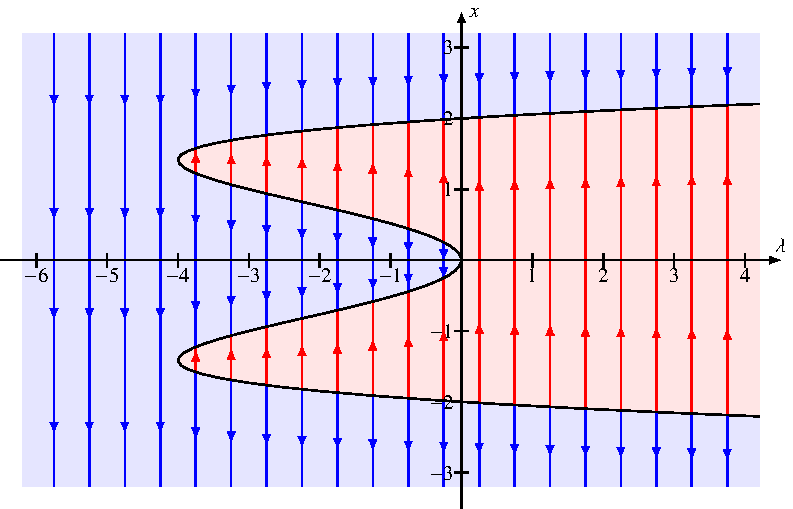
\includegraphics{chapters/3/grad4.pdf}
\caption{Phasendiagramm der Differentialgleichung~\eqref{aufgabe301:gl}.
\label{aufgabe301:fig}}
\end{figure}
\begin{teilaufgaben}
\item
Die kritischen Punkte der Differentialgleichung~\eqref{aufgabe301:gl}
sind Nullstellen der Gleichung
\begin{equation}
x^4-4x^2-\lambda=0
\label{aufgabe301:nullstellen}
\end{equation}
Dies ist eine quadratische Gleichung in $x^2$, die mit der Lösungsformel
für die quadratische Gleichung gelöst werden kann:
\[
x^2 = 2 \pm \sqrt{4+\lambda}.
\]
Diese Gleichung hat reelle Lösungen für $\lambda \ge -4$.
Für $\lambda \le 0$ ist die Quadratwurzel nicht grösser als $2$,
so dass die beiden Nullstellen positiv sind, es also vier verschiedene
Lösungen
\begin{equation}
x_{1,2,3,4} = \pm\sqrt{2\pm\sqrt{4+\lambda}}
\end{equation}
hat.
Für $\lambda >0$ hat die quadratische Gleichung eine negative Lösung
für $x^2$, die also nicht zu einer reellen Lösung der
Gleichung~\eqref{aufgabe301:nullstellen} führen kann.
Nur aus der positive Lösung $2+\sqrt{4+\lambda}$ kann man eine
Gleichgweichslösung, nämlich
\[
x=\pm\sqrt{2+\sqrt{4+\lambda}}
\]
ableiten.
Für $\lambda < -4$ gibt es gar keine Gleichgewichtslösung.

Das Phasendiagramm in Abbildung~\ref{aufgabe301:fig} zeigt,
dass für $\lambda >0$ die obere Gleichgewichtslösung stabil ist,
untere dagegen instabil.
Für $-4\le\lambda\le 0$ sind die Gleichgewichtslösungen
\begin{align*}
&\sqrt{2+\sqrt{4+\lambda}}
&&\text{und}&
&-\sqrt{2-\sqrt{4+\lambda}}
\\
\intertext{stabil und die Gleichgewichtslösungen}
&-\sqrt{2+\sqrt{4+\lambda}}
&&\text{und}&
&\sqrt{2-\sqrt{4+\lambda}}
\end{align*}
instabil.

Bei $\lambda=-4$ finden gleichzeitig zwei Sattel-Knoten-Bifurkationen 
statt, bei $\lambda=0$ findet ein einfache Sattel-Knoten-Bifurkation
statt, jedoch in umgekehrter Richtung wie im Beispiel im Text.
\item
Beim Anwachsen des Parameters über den Punkt $\lambda=0$ springt die
Gleichgewichtslösung auf die stabile Lösung
\[
x(\lambda)=\sqrt{2+\sqrt{4+\lambda}}.
\]
Bei der anschliessenden Verringerung von $\lambda$ bleibt die 
Gleichgewichtslösung auf dem Ast $x(\lambda)$ der Kurve, da diese
alle stabil sind.
Unabhängig vom Ausgangszustand befindet sich das System am Ende des
beschriebenen Szenarios also immer in der Nähe der Gleichgewichtslösung
\[
x(-1)=\sqrt{2+\sqrt{3}}.
\qedhere
\]
\end{teilaufgaben}
\end{loesung}


\end{uebungsaufgaben}

		% 6
%
% elnino.tex
%
% (c) 2018 Prof Dr Andreas Müller, Hochschule Rapperswil
%
\chapter{El Niño Southern Oscillation}
\lhead{El Niño Southern Oscillation}
Die Klimaentwicklung hängt wesentlich davon ab, wie Energie an der
Erdoberfläche verteilt wird.
Aus diesem Grund haben wir in Kapitel~\ref{chapter:fluiddynamik}
die Strömungsdynamik als den wesentlichen Mechanismus des 
Energietransportes in der Atmoshpäre studiert.
Und in Kapitel~\ref{chapter:thc} haben wir mit der Modellierung der
thermohalinen Zirkulation eine alternative Möglichkeit kennengelernt,
den Energie-Transport in den Weltmeeren zu beschreiben.

Das El Niño-Phänomen im Pazifik ist ein interessantes Teilsystem des
Klimasystems, welches einigermassen gut als isoliertes Teilsystem 
behandelt werden kann.
Die Modellierung, die wir in diesem Kapitel anstreben, braucht
einerseits die Ideen der Fluiddynamik, um die Energietransportmechanismen
zu beschreiben, und andererseits die Idee der Box-Modelle, um aus diesen
Mechanismen eine einfache gewöhnliche Differentiagleichung abzuleiten,
mit deren Hilfe die Dynamik des El~Niño studiert werden kann.

\section{El Niño}
\rhead{El Niño}

%
% kelvin.tex
%
% (c) 2018 Prof Dr Andreas Müller, Hochschule Rapperswil
%
\section{Kelvin-Wellen\label{section:elnino:kelvin}}
\rhead{Kelvin-Wellen}
In diesem Abschnitt soll die Ausbreitung von Anomalien in der Höhe
der Meeresoberfläche in der Nähe des Äquators studiert werden.

\subsection{Kelvin-Wellen\label{subsection:kelvin}}
\index{Kelvin-Wellen}
In der einfachsten Form führt ein Tiefdruckgebiet über dem zentralen
Pazifik dazu, dass die Meeresoberfläche über die Normalhöhe ansteigt.
Wenn sich das Tiefdruckgebiet auffüllt und die Druckkraft zur Aufrechterhaltung
dieser Anomalie wegfällt, wird dieser ``Wasserberg'' zerfallen.
Mit Hilfe der Gleichungen der Strömungsdynamik sollte sich die Ausbreitung
dieser Wellen beschreiben lassen.

Da die Anfangsbedingungen symmetrisch bezüglich einer Spiegelung an
der Äquatorebene sind, dürfen wir annehmen, dass auch die resultierende
Strömung diese Symmetrie hat.
In unmittelbarer Nähe des Äquators brauchen wir die Krümmung der
Erdoberfläche nicht zu berücksichtigen, und können daher mit einem
$x$-$y$-Koordinatensystem arbeiten, in dem $x$ die Richtung entlang des
Äquators und $y$ die Richtung entlang der Längenkreise ist (siehe auch
die Beschreibung der $\beta$-Ebene auf
Seite~\pageref{skript:betaplane:definition}).
\index{$\beta$-Ebene}%
Die Strömungsgeschwindigkeitskomponenten nennen wir $u$ entlang des
Äquators und $v$ entlang der Längenkreise.
Die Anomalie der Höhe der Meeresoberfläche bezeichnen wir mit $h(x,y)$.

\subsection{Bewegungsgleichung für Kelvin-Wellen}
Die zeitliche Änderung der Geschwindigkeit, also die Beschleunigung,
ist nach dem zweiten Newtonschen Gesetz proportional zu den Kräften.
Die Schwerkraft versucht, den Wasserberg abzubauen.
Wasser wird in diejenige Richtung beschleunigt, in die die Höhe $h(x,y)$
abnimmt.
Ausserdem wirkt die Coriolis-Kraft, die die Strömung auf der Nordhalbkugel
nach rechts ablenkt und auf der Südhalbkugel nach links.
So erhalten wir die Bewegungsgleichungen
\begin{equation}
\begin{aligned}
\frac{\partial u}{\partial t}
&=
\phantom{-}
fv - g\frac{\partial h}{\partial x}
\\
\frac{\partial v}{\partial t}
&=
-fu - g\frac{\partial h}{\partial y}.
\end{aligned}
\label{elnino:kelvin:newton}
\end{equation}
Dies ist ein System von zwei partiellen Differentialgleichung für 
drei unbekannte Funktionen $h$, $u$ und $v$, es ist also mindestens
noch eine weitere Gleichung nötig, damit das Problem überhaupt gelöst
werden kann.

Abfliessendes Wasser reduziert die Höhenanomalie.
Die Kontinuitätsgleichung~\eqref{skript:kontinuitaetsgleichung}
besagt, dass die Abnahme der Höhenanomalie $h$ proportional ist zur
Divergenz des Geschwindigkeitsfeldes.
Die fehlende Differentialgleichung ist daher
\begin{equation}
\frac{\partial h}{\partial t}
=
-H\biggl(
\frac{\partial u}{\partial x} + \frac{\partial v}{\partial y}
\biggr).
\label{elnino:kelvin:kont}
\end{equation}
Gesucht ist jetzt also eine Lösung der Differentialgleichungen
\eqref{elnino:kelvin:newton} und \eqref{elnino:kelvin:kont}.

\subsection{Wellengleichung}
Wir interessieren uns nur für eine Lösung in unmittelbarer Nähe des
Äquators und dürfen daher annehmen, dass sich das Wasser nicht
entlang der Längenkreise bewegt, dass also $v=0$ gilt.
Die Differentialgleichungen
\eqref{elnino:kelvin:newton} und \eqref{elnino:kelvin:kont}
vereinfachen sich damit zu
\begin{align}
\frac{\partial u}{\partial t}
&=
\phantom{-fu}
 - g\frac{\partial h}{\partial x}
\label{kelvin:naeherung:1}
\\
0
&=
-fu - g\frac{\partial h}{\partial y}
\label{kelvin:naeherung:2}
\\
\frac{\partial h}{\partial t}
&=
-H
\frac{\partial u}{\partial x}
\label{kelvin:naeherung:3}
\end{align}
Wir suchen nach einem Wellenphänomen entlang des Äquators, dafür
brauchen wir eine Wellengleichung in den Variablen $t$ und $x$,
die in den Gleichungen \eqref{kelvin:naeherung:1} nach
\eqref{kelvin:naeherung:3} vorkommen.
Aus diesen beiden Gleichungen sollte sich eine Wellengleichung
gewinnen lassen.

Indem wir \eqref{kelvin:naeherung:1} nach $x$ und 
\eqref{kelvin:naeherung:3} nach $t$ ableiten, erhalten wir
\begin{equation}
\left.
\begin{aligned}
\frac{\partial^2 u}{\partial x\,\partial t}
&=
-g\frac{\partial^2h}{\partial x^2}
\\
\frac{\partial^2 h}{\partial t^2}
&=
-H\frac{\partial^2 u}{\partial t\,\partial x}
\end{aligned}
\;
\right\}
\quad
\Rightarrow
\quad
\frac{\partial^2 h}{\partial t^2}
=
gH\frac{\partial^2 h}{\partial x^2}
\label{kelvin:wellengleichung}
\end{equation}
Dies ist die gesuchte Wellengleichung für eine Welle mit
Ausbreitungsgeschwindigkeit $c=\sqrt{gH}$.
Im nächsten Abschnitt bestimmen wir ihre Lösungen.

\subsection{Approximative Lösung der Wellengleichung}
Bis jetzt wurde die zweite Gleichung~\eqref{kelvin:naeherung:2}
nicht verwendet, es wurde eigentlich nur das Verhalten der Welle auf
dem Äquator modelliert.
Da wir jetzt aber wissen, dass mindestens entlang des Äquators die Lösung
eine Welle mit Ausbreitungsgeschwindigkeit $c=\sqrt{gH}$ ist, können
wir versuchen, auch die $y$-Abhängigkeit zu modellieren.

\subsubsection{Dispersionsrelation}
Eine in $x$-Richtung laufende Welle mit Wellenzahl $k$ kann beschrieben werden
als $\cos(kx-\omega t)$.
Die Wellenzahl $k$ ist positiv für eine nach Osten laufende Welle und negativ
für eine nach Westen laufende Welle.
Überall dort, wo $kx-\omega t=0$ ist, befindet sich ein Wellenberg,
die Position dieses Maximums ist also
\[
x=\frac{\omega}{k}\cdot t,
\]
es bewegt sich also mit der Geschwindigkeit $c=\omega/k$.
Dies ist die sogenannte {\em Phasengeschwindigkeit}.
\index{Phasengeschwindigkeit}%

Wir dürfen allerdings nicht davon ausgehen, dass das Verhältnis $\omega/k$
konstant ist, Wellen mit verschiedenen Frequenzen können sich durchaus
mit verschiedenen Geschwindigkeiten ausbreiten.
Ein Glasprisma ist in der Lage, Licht in seine verschiedene Farben
mit verschiedenen Ausbreitungsgeschwindigkeiten im Glas aufzufächern. 
Dieses Phänomen heisst {\em Dispersion} und äussert sich in einem
\index{Dispersion}%
funktionalen Zusammenhang
\[
\omega = \omega(k)
\]
zwischen Wellenzahl $k$ und Frequenz $\omega$, einer {\em Dispersionsrelation}.
\index{Dispersionsrelation}%

Wir suchen also eine Lösung des Gleichungssystems
\eqref{kelvin:naeherung:1}--\eqref{kelvin:naeherung:3}
in der Form
\[
h_k(t,x,y) = \gamma(y)\cdot \cos(kx-\omega t)
\]
zu finden.
Die Funktion $\gamma(y)$ beschreibt das Profil des ``Wasserberges'' 
in der Nähe des Äquators, wir nehmen daher an, dass $\gamma(y)$ für grosse
Werte von $y$ rasch abnimmt.

Einsetzen des Lösungsansatzes $h_k(t,x,y)$ in die
Gleichung~\eqref{kelvin:wellengleichung} liefert
\begin{equation}
\left.
\begin{aligned}
\frac{\partial^2 h_k}{\partial t^2}
&=
- \omega^2 \gamma(y) \cos(kx-\omega t)
=
-\omega^2 h_k(t,x,y)
\\
\frac{\partial^2 h_k}{\partial x^2}
&=
-
k^2
\gamma(y)
\cos (kx-\omega t)
=
-k^2 h_k(t,x,y)
\end{aligned}
\;\right\}
\quad
\Rightarrow
\quad
\omega^2=gHk^2
\quad\text{oder}\quad
\biggl|
\frac{\omega}{k}\biggr|
=\sqrt{gH}=c
\end{equation}
Aus dieser Dispersionsrelation
liest man ab, dass die Phasengeschwindigkeit einer solchen
Welle unabhängig ist von der Frequenz.

\subsubsection{$y$-Abhängigkeit}
Bis jetzt haben wir die Gleichung~\eqref{kelvin:naeherung:2} nicht
verwendet.
Sie erlaubt, $u$ zu berechnen, es gilt
\[
u=-\frac{g}{f}\,\frac{\partial h}{\partial y}
\qquad
\text{oder für $h_k$}
\qquad
u_k=-\frac{g}{f} \gamma'(y) \sin(kx-\omega t).
\]
Setzt man dies in \eqref{kelvin:naeherung:3} ein, erhält man
\begin{equation}
\left.
\begin{aligned}
\frac{\partial h_k}{\partial t}
&=
-\omega
\gamma(y) \cos(kx-\omega t)
\\
\frac{\partial u_k}{\partial x}
&=
k \frac{g}{f}\gamma'(y) \cos(kx-\omega t)
\end{aligned}
\;\right\}
\qquad\Rightarrow\qquad
-\omega
\gamma(y) \cos(kx-\omega t)
=
-H
k \frac{g}{f}\gamma'(y) \cos(kx-\omega t).
\end{equation}
Nach Kürzen gemeinsamer Faktoren und Umstellen folgt
\begin{equation}
\gamma'(y)
=
\gamma(y) \frac{f}{gH}\frac{\omega}{k}
=
\pm
\frac{f}{c} \gamma(y).
\label{kelvin:gamma:dgl1}
\end{equation}
Das Vorzeichen in \eqref{kelvin:gamma:dgl1} hängt vom Vorzeichen der
Wellenzahl $k$ ab, das obere Vorzeichen steht für eine nach Osten
laufende Welle.

Die Coriolis-Kraft $f$ verschwindet am Äquator, in erster Näherung
ist sie proportional zu $y$, wir schreiben daher $f=\beta y$.
Die Differentialgleichung~\eqref{kelvin:gamma:dgl1} wird damit zu
\begin{equation}
\gamma'(y)
=
\pm
\frac{\beta}{c} 
y\gamma(y).
\label{kelvin:gamma:dgl2}
\end{equation}

Für zunehmende $y$ muss $\gamma$ abnehmen, es muss also $\gamma'(y)<0$ sein
für genügend grosse $y$.
Dies ist aber nur möglich für das negative Vorzeichen, und damit nur
für eine nach Osten laufende Welle.
Im Folgenden konzentrieren wir uns daher auf das negative Zeichen
in \eqref{kelvin:gamma:dgl2}.

Um eine Lösung von \eqref{kelvin:gamma:dgl2} zu finden, teilen wir
durch $\gamma(y)$
und verwenden, dass $\gamma'(y)/\gamma(y)$ die Ableitung des
Logarithmus ist:
\begin{equation}
\frac{\gamma'(y)}{\gamma(y)}
=
\frac{d}{dy}\log \gamma(y) = -\frac{\beta}{c} y
\qquad\Rightarrow\qquad
\log\gamma(y) = -\frac{\beta}{2c}y^2
\qquad\Rightarrow\qquad
\gamma(y) = \exp\biggl(
- \frac{\beta}{2c}y^2
\biggr)
\end{equation}
Das $y$-Profil der Welle ist also eine Gauss-Funktion.
Die Zone, in der sich eine Kelvin-Welle ausbreiten kann, 
wird schmaler, wenn $\beta$ grösser wird, wenn also die 
Rotationsgeschwindigkeit des Planeten grösser wird.
Sie wird kleiner, wenn $c=\sqrt{gH}$ grösser wird, also
bei grösserer Gravitation.


%
% rossby.tex
%
% (c) 2018 Prof Dr Andreas Müller, Hochschule Rapperswil
%

\section{Rossby-Wellen\label{section:elnino:rossby}}
\rhead{Rossby-Wellen}
In der Untersuchung der Kelvin-Wellen haben wir angenommen, dass die
Geschwindigkeit $v$ entlang der Längenkreise verschwindet.
Die Strömung wird aber im Allgemeinen nicht parallel zum Äquator sein.
Wir beobachten zum Beispiel, dass die Westwindströmung 
zwischen verschiedenen geographischen Breiten mäandriert.
Woher kommt diese Wellenbewegung?
\index{Rossby-Wellen}%

\subsection{Zirkulation\label{subsection:rossby:zirkulation}}
Aus der Diskussion der globalen Zirkulation in
Kapitel~\ref{chapter:wetter und klima} wissen wir, dass die
Strömung in Äquatornähe dominiert wird durch eine mittlere
konstante Strömung mit Geschwindigkeit $U$ in Ost-West-Richtung.
Wir suchen daher eine Beschreibung der Abweichungen von dieser
mittleren Strömung.
Unter Verwendung der gleichen Notation wie im
Abschnitt~\ref{section:elnino:kelvin} schreiben wir daher
\[
u'=U+u,\qquad v'=v\qquad\text{mit $u,v\ll U$}.
\]
Die Geschwindigkeitskomponenten $u$ und $v$ sind die Anomalien relativ
zur vorherrschenden mittleren Strömung.

Wir nehmen im Folgenden wieder an, dass die Strömung quellenfrei ist.
Dann lässt sich wie früher gezeigt die Strömung mit einer
Strömungsfunktion $\psi$ als
\begin{equation}
u=-\frac{\partial \psi}{\partial y},\qquad
v=\frac{\partial\psi}{\partial x}
\label{skript:rossby:geschwindigkeit}
\end{equation}
beschreiben.

Die gesuchten Wellen sollen Mäander-Form der Strömung erklären,
also Änderungen der Strömungsrichtungen, die natürlich mit
Änderungen des Drehimpulses einhergehen.
Die Drehimpulsdichte in der Strömung ist gegeben durch die Zirkulation
\[
\zeta
=
\frac{\partial v}{\partial x} - \frac{\partial u}{\partial y}
=
\Delta \psi.
\]
Da der Drehimpuls erhalten ist, muss die Zirkulation in einem
Luftpaket abnehmen, wenn es sich auf der Nordhalbkubel nach Norden
bewegt.
Die Quelle dieser Zirkulationsänderung ist die Erddrehung und damit
die Corioliskraft $f$ und der mathematische Ausdruck der Drehimpulserhaltung
ist die Erhaltung der Grösse $\zeta+f$.

\subsection{Bewegungsgleichung\label{subsection:rossby:bewegungsgleichung}}
Die Grösse $\zeta+f$ ist erhalten, daher muss ihre zeitliche Ableitung
\[
\frac{d(\zeta f)}{dt}=0
\]
verschwinden.
Die Coriolis-Kraft
$f$ hängt nur von $y$ ab, aber die Funktion $\zeta$ hängt von allen
drei Variablen $t$, $x$ und $y$ ab.
Wir berechnen die Ableitung mit Hilfe der Kettenregel:
\begin{align*}
0
=
\frac{d(\zeta+f)}{dt}
&=
\frac{\partial\zeta}{\partial t}
+
\frac{\partial\zeta}{\partial x}\cdot \frac{dx}{dt}
+
\frac{\partial(\zeta+f)}{\partial y}\cdot\frac{dy}{dt}
\\
&\simeq
\frac{\partial\zeta}{\partial t}
+
(U+u)\frac{\partial\zeta}{\partial x}
+
v\biggl(\frac{\partial\zeta}{\partial y} + \frac{\partial f}{\partial y}\biggr).
\end{align*}
Da $u\ll U$ ist, können wir in erster Näherung $u$ im zweiten Term 
vernachlässigen.
Und da $\partial\zeta/\partial y$ ebenfalls sehr klein ist, können
wir dies im letzten Term im Vergleich zu $\partial f/\partial y$
vernachlässigen.
Schliesslich können wir wie in Abschnitt~\ref{section:elnino:kelvin}
die $\beta$-Ebenen-Approximation verwenden und $\partial f/\partial y$
durch $\beta$ ersetzen.
Schliesslich können wir wieder mit \eqref{skript:rossby:geschwindigkeit}
$v$ als Ableitung von $\psi$ nach $x$ ausdrücken.
Wir erhalten so
\[
0
=
\frac{\partial\zeta}{\partial t}
+
U\frac{\partial\zeta}{\partial x}
+
\beta\frac{\partial\psi}{\partial x}
\]
als Bewegungsgleichung.

Indem wir $\zeta=\Delta \psi$ schreiben, erhalten wir so die 
Bewegungsgleichung
\begin{equation}
\frac{\partial\Delta\psi}{\partial t}
+
U\frac{\partial\Delta\psi}{\partial x}
+
\beta\frac{\partial\psi}{\partial x}
=
0.
\label{rossby:gleichung}
\end{equation}


\subsection{Wellenlösungen\label{subsection:rossby:loesungen}}
Gesucht sind Lösungen der Gleichung~\eqref{rossby:gleichung}
in Form kleiner Abweichungen.
Wir erwarten Wellenlösungen und schreiben sie daher in der Form
\begin{equation}
\psi_{kl}(t,x,y)
=
\cos(kx+ly-\omega t).
\label{rossby:ebenewelle}
\end{equation}
Die Ableitungen, die wir für die Bewegungsgleichung
\eqref{rossby:gleichung} benötigen, sind
\begin{align*}
\frac{\partial}{\partial t} \psi_{kl}(t,x,y)
&=
\omega \sin(kx+ly-\omega t)
\\
\frac{\partial}{\partial x} \psi_{kl}(t,x,y)
&=
-k
\sin(kx+ly-\omega t)
\\
\Delta\psi_{kl}
&=
-(k^2+l^2)\cos(kx+ly-\omega t)=-(k^2+l^2)\psi_{kl}(t,x,y).
\end{align*}
Setzen wir dies in die Differentialgleichung
\eqref{rossby:gleichung}
ein, erhalten wir 
\begin{align*}
0
&=
-
\omega(k^2+l^2) 
\sin(kx+ly-\omega t)
+
Uk(k^2+l^2)
\sin(kx+ly-\omega t)
-
\beta k
\sin(kx+ly-\omega t)
\\
&=
-\bigl((\omega-Uk)(k^2+l^2)+\beta k\bigr)
\sin(kx+ly-\omega t).
\end{align*}
Für eine Lösung muss also die Dispersionsrelation
\[
(\omega -Uk)(k^2+l^2) +\beta k=0
\]
gelten.
Aufgelöst nach $\omega$ ist dies
\begin{align}
\omega(k^2+l^2)
&=
Uk(k^2+l^2) -\beta k
\notag
\\
\Rightarrow\qquad
\omega
&=
Uk
-
\frac{\beta k}{k^2+l^2}.
\label{rossby:dispersion}
\end{align}
Eine Wellenlösung mit Wellenzahlen $k$ und $l$ hat daher 
die Ausbreitungsgeschwindigkeit 
\begin{equation}
c=\frac{\omega}{k} = U-\beta\frac{1}{k^2+l^2}
\label{rossby:phasengeschwindigkeit}
\end{equation}
entlang der $x$-Koordinate.
Da der Nenner immer positiv ist, ist $c$ kleiner als $U$, solche
Wellen können sich immer nur in West-Ost-Richtung ausbreiten.

\subsection{Gruppengeschwindigkeit}
Die Phasengeschwindigkeit~\eqref{rossby:phasengeschwindigkeit}
hilft uns nicht, die Dynamik des El Niño zu verstehen, da wir dazu
den Transport von Energie verstehen müssen.
Die ebenen Wellen der Form~\eqref{rossby:ebenewelle} beschreiben eine Welle,
die überall die gleiche Amplitude hat.
Ein Transport von potentieller Energie findet aber nur statt, wenn ein
``Wellenberg'' sich an einen anderen Ort bewegt.
Im Beispiel des ``Wasserberges'' in der Untersuchung zu den Kelvin-Wellen
wird potentielle Energie dadurch transportiert, dass das Wasser des Berges
abfliesst.
Wir müssen daher erst einen ``Wasserberg'' als Überlagerung von 
ebenen Wellen formulieren und dann die zeitliche Entwicklung dieser
Überlagerung studieren.

\subsubsection{Überlagerungen}
Wir gehen von einer eindimensionalen Situation aus und studieren
eine Überlagerung $u(x,t)$ von Wellen der Form $\cos(kx-\omega(k) t)$
mit verschiedenen Wellenzahlen $k$.
Mit der wellenzahlabhängigen Amplitude $\hat f(k)$, dem Spektrum
wie in Kapitel~\ref{chapter:fourier} studiert, lässt sich die
Überlagerung als
\begin{equation}
u(x,t)
=
\int_{-\infty}^\infty \hat f(k)\,\cos(kx-\omega(k)t)\,dk
\label{rossby:reelleueberlagerung}
\end{equation}
schreiben.
Die Bewegung eines solchen Wellenpaketes kann man zum Beispiel
dadurch studieren, dass man die Bewegung des Maximums dieses 
Wellenpaketes verfolgt.
\index{Wellenpaket}

Die Darstellung~\eqref{rossby:reelleueberlagerung} ist für diese
Untersuchung sehr unhandlich, die Rechnungen sind zu umständlich.
Wir schreiben die Wellen daher als Realteil einer komplexen
Welle $e^{i(kx-\omega(k)t)}$, also
\begin{equation}
u(x,t)
=
\operatorname{Re}
\int_{-\infty}^\infty \hat f(k)\,e^{i(kx-\omega(k)t)}\,dk.
\label{rossby:komplexeueberlagerung}
\end{equation}
Dabei lassen wir auch zu, dass $\hat{f}(k)$ komplexe Werte annimmt.

\subsubsection{Wellenpakete}
\begin{figure}
\centering
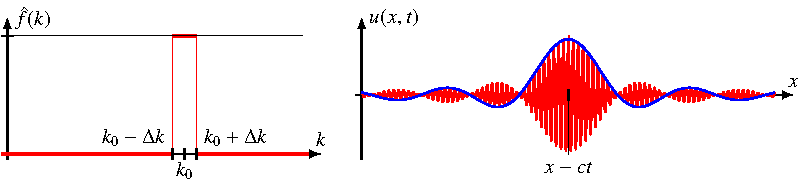
\includegraphics{chapters/7/wellenpaket.pdf}
\caption{Berechnung eines Wellenpaketes aus Wellen mit Wellenzahlen
zwischen $k_0-\Delta k$ und $k_0+\Delta k$.
\label{rossby:wellenpaket}}
\end{figure}
Wir betrachten ein Wellenpaket, welches als Überlagerung mit der
Amplitudenfunktion
\[
\hat f(k)
=
\begin{cases}
1&\qquad |k-k_0| < \Delta k\\
0&\qquad\text{sonst}
\end{cases}
\]
wie in Abbildung~\ref{rossby:wellenpaket} entsteht.
Die Überlagerung $u(x,t)$ gemäss~\eqref{rossby:komplexeueberlagerung}
kann man jetzt vereinfachen:
\[
u(x,t)
=
\operatorname{Re}
\int_{-\infty}^\infty \hat f(k)\,e^{i(kx-\omega(k)t)}\,dk
=
\operatorname{Re}
\int_{k_0-\Delta k}^{k_0+\Delta k} e^{i(kx-\omega(k)t)}\,dk,
\]
allerdings muss dazu $\omega(k)$ bekannt sein.

Falls $\omega(k)=ck$ gilt, falls also jede der elementaren Wellen
$\cos(kx-\omega t)$ die gleiche
Ausbreitungsgeschwindigkeit $c$ hat, können wir $u(x,t)$ explizit
ausrechnen:
\begin{align*}
u(x,t)
&=
\operatorname{Re}
\int_{k_0-\Delta k}^{k_0+\Delta k}
e^{i(kx-\omega(k)t)}\,dk
=
\operatorname{Re}
\int_{k_0-\Delta k}^{k_0+\Delta k}
e^{ik(x-ct)}\,dk
\\
&=
\operatorname{Re}
\biggl[
\frac{e^{ik(x-ct)}}{i(x-ct)}
\biggr]_{k_0-\Delta k}^{k_0+\Delta k}
=
\operatorname{Re}
\biggl(
\frac{e^{i(k_0+\Delta k)(x-ct)}}{i(x-ct)}
-
\frac{e^{i(k_0-\Delta k)(x-ct)}}{i(x-ct)}
\biggr)
\\
&=
\operatorname{Re}\frac{2}{x-ct}
e^{ik_0(x-ct)}\frac{e^{i\Delta k(x-ct)}-e^{i\Delta k(x-ct)}}{2i}
\\
&=
\operatorname{Re}\frac{2}{x-ct}
e^{ik_0(x-ct)}
\sin (\Delta k(x-ct))
=
2\cos k_0(x-ct) \frac{\sin \Delta k(x-ct)}{x-ct}
\end{align*}
Dies ist eine schnell schwankende Funktion mit Wellenzahl $k_0$, rot
dargestellt in Abbildung~\ref{rossby:wellenpaket} rechts, moduliert
mit der langsam schwankenden Funktion $\sin\Delta k(x-ct)/(x-ct)$,
dargestellt in der selben Abbildung in blau.
Der Schwerpunkt des Paketes befindet sich bei der $x$-Koordinaten $x-ct$,
er wandert also mit Geschwindigkeit $c$ nach rechts.

\subsubsection{Gruppengeschwindigkeit}
\index{Gruppengeschwindigkeit}%
Bisher haben wir angenommen, dass die Frequenz und die Wellenzahl proportional
sind, dass also $\omega(k)=ck$.
Die Untersuchungen zu den Rossby-Wellen hat gezeigt, dass dies nicht
zutreffen muss.
Wir müssen die Rechnung also mit einem Modell wiederholen, in dem die
Frequenz $\omega(k)$ nicht einfach nur proportional zu $k$ ist.
Für kleines $\Delta k$ genügt eine lineare Approximation der
Abhängigkeit von $\omega(k)$ von $k$, wir setzen daher
\begin{equation}
\omega(k)
=
\omega(k_0) + (k-k_0)\omega_1
=
\omega_0 + (k-k_0)\omega_1
\qquad
\text{mit}
\quad
\omega_1 = \frac{d}{dk}\omega(k_0) = \omega'(k_0).
\end{equation}
Wir berechnen wieder $u(x,t)$ wie folgt:
\begin{align*}
u(x,t)
&=
\operatorname{Re}
\int_{k_0-\Delta k}^{k_0+\Delta k}
e^{i(kx-\omega(k)t}\,dk
=
\operatorname{Re}
\int_{k_0-\Delta k}^{k_0+\Delta k}
e^{i(kx-\omega_0t -\omega_1(k-k_0)t)}
\,dk
\\
&=
\operatorname{Re}
\int_{k_0-\Delta k}^{k_0+\Delta k}
e^{i(k(x-\omega_1 t)-\omega_0t +\omega_1k_0t)}
\,dk
=
\operatorname{Re}
\int_{k_0-\Delta k}^{k_0+\Delta k}
e^{ik(x-\omega_1 t)}
e^{i(\omega_1k_0-\omega_0)t}
\,dk
\\
&=
\operatorname{Re}
e^{i(\omega_1k_0-\omega_0)t}
\biggl[
\frac{e^{ik(x-\omega_1 t)}}{i(x-\omega_1 t)}
\biggr]_{k_0-\Delta k}^{k_0+\Delta k}
=
\operatorname{Re}
2e^{i(\omega_1k_0-\omega_0)t}
\frac{
e^{i(k_0+\Delta k)(x-\omega_1 t)}
-
e^{i(k_0-\Delta k)(x-\omega_1 t)}
}{2i(x-\omega_1 t)}
\\
&=
\operatorname{Re}
\frac{2e^{i(\omega_1k_0-\omega_0)t}e^{i(k_0(x-\omega_1 t))}}{x-\omega_1 t}
\frac{
e^{i\Delta k(x-\omega_1 t)}
-
e^{-i\Delta k(x-\omega_1 t)}
}{2i}
=
\operatorname{Re}
2e^{i(\omega_1k_0-\omega_0+k_0(x-\omega_1 t))}
\frac{\sin \Delta k(x-\omega_1t)}{x-\omega_1 t}
\\
&=
\operatorname{Re}
2e^{i(k_0x-\omega_0t)}\,
\frac{\sin \Delta k(x-\omega_1t)}{x-\omega_1 t}
=
2\cos(k_0x-\omega_0t)
\frac{\sin \Delta k(x-\omega_1t)}{x-\omega_1 t}.
\end{align*}
Wiederum erhalten wir eine kurze Welle mit Frequenz
$\omega_0$ und Wellenzahl $k_0$, die moduliert wird mit der langsam
schwankenden Funktion
\begin{equation}
\frac{\sin\Delta k(x-\omega_1t)}{x-\omega_1 t}.
\label{rossby:gruppe}
\end{equation}
Das Maximum der Funktion~\eqref{rossby:gruppe}
befindet sich bei $x=\omega_1 t$, wandert also mit der
Geschwindigkeit $\omega_1$ nach rechts.

Die soeben durchgeführte Berechnung zeigt also, dass Wellenpakete
mit der Geschwindigkeit 
\[
c_g=\frac{d\omega(k)}{dk},
\]
der sogenannten {\em Gruppengeschwindigkeit}, wandern.
\index{Gruppengeschwindigkeit}%
Der Energietransport durch Wellenpakete erfolgt offenbar nicht
mit der Ausbreitungsgeschwindigkeit $c=\omega/k$, sondern mit der
Gruppengeschwindigkeit.

\subsection{Energietransport durch Rossby-Wellen\label{rossby:transport}}
Aus der Dispersionsrelation~\eqref{rossby:dispersion}
für die Rossby-Wellen können wir jetzt die Gruppengeschwindigkeit
für parallel zum Äquator sich bewegende Wellenpakete
durch Ableiten nach $k$ bestimmen.
Die Gruppengeschwindigkeit ist
\begin{equation}
c_g
=
\frac{d}{dk}\omega(k)
=
U-\beta
\frac{k^2+l^2-k\cdot 2k}{(k^2+l^2)^2}
=
U-\beta
\frac{l^2-k^2}{(k^2+l^2)^2}
\end{equation}
Je nach der relativen Grösse von $k$ und $l$ kann die
Gruppengeschwindigkeit sowohl grösser als auch kleiner sein als die
mittlere Geschwindigkeit $U$ in der Zone.
Rossby-Wellen können also je nach Wellenzahl sowohl nach Westen wie
auch nach Osten laufen.








%
% verzoegert.tex
%
% (c) 2018 Prof Dr Andreas Müller, Hochschule Rapperswil
%
\section{Verzögertes Oszillator-Modell\label{section:dde-nino}}
In den Kelvin- und Rossby-Wellen haben wir Mechanismen kennengelernt,
die Energietransport entlang des Äquators innerhalb der vorherrschenden
Strömung sowohl in östlicher wie auch in westlicher Richtung ermöglichen.
Entscheidend für die Dynamik dieses Energietransports ist die Zeit,
die eine Welle benötigt, um den Pazifik zu durchqueren.
Sei $\tau_K$ die Zeit, die eine Kelvin-Welle braucht, um den Pazifik
zu durchqueren, und $\tau_R$ die entsprechende Zeit für eine Rossby-Welle.

\rhead{Verzögertes Oszillator-Modell}
Wir versuchen jetzt, ein für die Temperaturanomalie $T(t)$ im östlichen
Pazifik aufzustellen, die diese Mechanismen berücksichtigt.
Ohne einen Transportmechanismus würde die Temperaturanomalie einfach
zerfallen, was beschrieben werden kann mit einer Differentialgleichung
der Form
\[
\frac{d}{dt}T(t)
=
-cT(t),
\]
mit einer Konstanten $c$.

\def\halb{\bgroup\textstyle\frac12\egroup}

Die Diskussionen über die dem El~Niño-Phänomen zugrunde liegenden
Mechanismen haben wir gesehen, dass die Thermoklinenanomalie im
zentralen Pazifik eine Auswirkung auf Temperatur\-anomalie $T(t)$ hat.
Eine Thermoklinenanomalie $h_0(t)$ am Äquator wandert als
Kelvin-Welle in der Zeit $\frac12\tau_K$ in den Ostpazifik.
Eine Thermoklinenanomalie $h_1(t)$ nördlich oder südlich des Äquators
kann als Rossby-Welle nach Westen wandern, am Westrand des Pazifik
reflektiert werden und als Kelvin-Welle in den Ostpazifik zurückkehren.
Dazu ist die Zeit $\frac12\tau_R+\tau_K$ nötig.
Dies lässt sich mit der Differentialgleichung
\begin{equation}
\frac{d}{dt}T(t)
=
-cT(t) + a_0h_0(t-\halb\tau_K) + b_0h_1(t-(\halb\tau_R+\tau_K))
\label{elninodde:1}
\end{equation}
erreichen.

Nun scheint es aber auch einen Zusammenhang zwischen der Temperaturanomalie
im Ostpazifik und den Thermoklinenanomalien im zentralen Pazifik zu geben.
Im einfachsten Fall kännen wir diesen Zusammenhang linear modellieren,
also 
\[
h_0(t-\halb\tau_K)
\sim
T(t-\halb\tau_K),
\qquad
\text{und}
\qquad
h_1(t-(\halb\tau_R+\tau_K))
\sim
T(t-(\halb\tau_R+\tau_K)).
\]
Eingesetzt in die Differentialgleichung~\eqref{elninodde:1} wird dabei zu
\begin{equation}
\frac{d}{dt}T(t)
=
-cT(t) + aT(t-\halb\tau_K) + bT(t-(\halb\tau_R+\tau_K))
\label{elninodde:2}
\end{equation}
Die Ableitung $\dot T(t)$ hängt also nicht nur von der Temperaturanomalie
zur Zeit $t$ ab, sondern auch von den Temperaturanomalien zu den
früheren Zeitpunkten $t-\halb\tau_K$ und $t-(\halb\tau_R-\tau_K)$.
Man nennt
\eqref{elninodde:2}
eine verzögerte Differentialgleichung.
\index{verzögerte Differentialgleichung}%

Die Theorie der linearen, verzögerten Differentialgleichungen wie 
\eqref{elninodde:2} zeigt, dass sie ähnlich wie gewöhnliche linear
Differentialgleichungen erster Ordnung Lösungen haben, die exponentiell
schnell zerfallen oder exponentiell anwachsen.
Daher können wir nicht erwarten, dass \eqref{elninodde:2} das El~Niño-Phänomen
adäquat beschreiben kann.
Um das exponentielle Anwachsen zu verhindern, braucht es einen zusätzlichen
Term, der dem Anwachsen von $T(t)$ überproportional entgegenwirkt.
Zum Beispiel könnte dies man mit einem Term der Form $-\varepsilon T(t)^3$
erreichen.
Die verzögerte Differentialgleichung ist dann
\begin{equation}
\frac{d}{dt}T(t)
=
-cT(t) + aT(t-\halb\tau_K) + bT(t-(\halb\tau_R+\tau_K))
-\varepsilon T(t)^3.
\label{elninodde:3}
\end{equation}
Ein andere Möglichkeit, ein ähnliches Ziel zu erreichen, wird in Kapitel
\ref{chapter:planeten} dargestellt.

In Kapitel~\ref{chapter:verzoegert} wird das Verhalten der Lösungen
solcher verzögerter Differentialgleichungen etwas mehr im Detail
diskutiert und es wird gezeigt, dass sie tatsächlich wesentliche
Aspekte des El~Niño-Phänomens adäquat wiedergeben können.









		% 7
%
% assim.tex
%
% (c) 2018 Prof Dr Andreas Müller, Hochschule Rapperswil
%
\chapter{Datenassimilation}
		% 8
